\documentclass{report}
% !TeX root = main.tex

% ----------------- Packages ----------------------
\usepackage{packages}

% ----------------- Thesis Information ----------------------
\title{Evaluating the Robustness of AI-Based Forensic Tools under Adversarial and Anti-Forensic Attacks}
\author{Lello Molinario}
\date{25/05/2026}

\begin{document}

% ============================================================
% Front Matter
% ============================================================

\pagenumbering{roman}
\pagestyle{frontmatterstyle}

% ----------------- Acronyms and Glossary Definitions ----------------------

% ─────────────────────────────────────────────────────────────────────────────
% General AI, ML and Digital Forensics terminology
% ─────────────────────────────────────────────────────────────────────────────

\newacronym{ai}{AI}{Artificial Intelligence}
\newacronym{ml}{ML}{Machine Learning}
\newacronym{dl}{DL}{Deep Learning}
\newacronym{advml}{Adv-ML}{Adversarial Machine Learning}
\newacronym{df}{DF}{Digital Forensics}
\newacronym{auroc}{AUROC}{Area Under the Receiver Operating Characteristic Curve}

% ─────────────────────────────────────────────────────────────────────────────
% Machine learning models and techniques
% ─────────────────────────────────────────────────────────────────────────────

\newacronym{cnn}{CNN}{Convolutional Neural Network}
\newacronym{svm}{SVM}{Support Vector Machine}
\newacronym{vit}{ViT}{Vision Transformer}
\newacronym{clip}{CLIP}{Contrastive Language-Image Pre-training}
\newacronym{blip}{BLIP}{Bootstrapping Language-Image Pre-training}
\newacronym{xai}{xAI}{Explainable Artificial Intelligence}
\newacronym{ood}{OOD}{Out-of-Distribution}

% ─────────────────────────────────────────────────────────────────────────────
% Adversarial Machine Learning terminology
% ─────────────────────────────────────────────────────────────────────────────

\newacronym{fgsm}{FGSM}{Fast Gradient Sign Method}
\newacronym{pgd}{PGD}{Projected Gradient Descent}

% ─────────────────────────────────────────────────────────────────────────────
% Image forensics and file formats
% ─────────────────────────────────────────────────────────────────────────────

\newacronym{jpeg}{JPEG}{Joint Photographic Experts Group}
\newacronym{png}{PNG}{Portable Network Graphics}
\newacronym{cgi}{CGI}{Computer-Generated Imagery}
\newacronym{prnu}{PRNU}{Photo Response Non-Uniformity}

% ─────────────────────────────────────────────────────────────────────────────
% Evaluation metrics and robustness analysis
% ─────────────────────────────────────────────────────────────────────────────

\newacronym{tp}{TP}{True Positive}
\newacronym{tn}{TN}{True Negative}
\newacronym{fp}{FP}{False Positive}
\newacronym{fn}{FN}{False Negative}
\newacronym{fpr}{FPR}{False Positive Rate}
\newacronym{fnr}{FNR}{False Negative Rate}

% ─────────────────────────────────────────────────────────────────────────────
% Explainability terminology
% ─────────────────────────────────────────────────────────────────────────────

\newacronym{ig}{IG}{Integrated Gradients}

% ─────────────────────────────────────────────────────────────────────────────
% Hashing, traceability and technical identifiers
% ─────────────────────────────────────────────────────────────────────────────

\newacronym{md5}{MD5}{Message Digest Algorithm 5}
\newacronym{sha256}{SHA-256}{Secure Hash Algorithm 256-bit}

% ─────────────────────────────────────────────────────────────────────────────
% Tools, standards and institutional references
% ─────────────────────────────────────────────────────────────────────────────

\newacronym{osint}{OSINT}{Open Source Intelligence}
\newacronym{ufed}{UFED}{Universal Forensic Extraction Device}
\newacronym{gdpr}{GDPR}{General Data Protection Regulation}
\newacronym{fairlab}{FAIRLab}{Forensic AI Robustness Lab}
\newacronym{gpu}{GPU}{Graphics Processing Unit}

% ─────────────────────────────────────────────────────────────────────────────
% Commercial forensic tools and AI-based forensic modules
% ─────────────────────────────────────────────────────────────────────────────

\newglossaryentry{magnetai}{
    name={Magnet.AI},
    text={Magnet.AI},
    description={AI-based image categorization module integrated in Magnet AXIOM}
}

\newglossaryentry{magnetaxiomtool}{
    name={Magnet AXIOM},
    description={commercial digital forensics platform used in this thesis through its Magnet.AI image categorization functionality}
}

\newglossaryentry{griffeye}{
    name={Magnet Griffeye},
    description={commercial forensic media-triage platform evaluated in this thesis as a black-box tool through automatic semantic bookmarks generated by T3K CORE}
}

\newglossaryentry{t3kcore}{
    name={T3K CORE},
    description={AI-assisted semantic-bookmark module used with Magnet Griffeye to generate automatic media-analysis bookmarks}
}


\newglossaryentry{excirefoto2025}{
    name={Excire Foto 2025},
    description={standalone general-purpose image management software with AI-based semantic search capabilities, evaluated in this thesis as a black-box retrieval system through an explicit operational normalization of its observable outputs}
}

\newglossaryentry{cellebriteinseyets}{
    name={Cellebrite Inseyets},
    description={commercial AI-assisted media analysis platform evaluated in this thesis as a black-box tool through the observable outputs exported in Cellebrite Physical Analyzer}
}


% ─────────────────────────────────────────────────────────────────────────────
% Adversarial attacks and anti-forensic transformations
% ─────────────────────────────────────────────────────────────────────────────

\newglossaryentry{onepixel}{
    name={One Pixel Attack},
    text={One Pixel Attack},
    description={adversarial attack based on sparse pixel-level perturbations}
}

\newglossaryentry{sigmazero}{
    name={Sigma Zero Attack},
    text={Sigma Zero Attack},
    description={sparse adversarial attack based on differentiable approximation of the \(L_0\) norm}
}

\newglossaryentry{superdeepfool}{
    name={SuperDeepFool},
    text={SuperDeepFool},
    description={iterative adversarial attack inspired by decision-boundary crossing methods}
}

\newglossaryentry{colorshift}{
    name={Color Shift},
    text={Color Shift},
    description={model-agnostic color perturbation applied to the image channels}
}

\newglossaryentry{jpegrecompression}{
    name={JPEG recompression},
    text={JPEG recompression},
    description={anti-forensic transformation based on lossy recompression of the image}
}

\newglossaryentry{resampleresize}{
    name={Resample + Resize},
    text={Resample + Resize},
    description={anti-forensic transformation based on downsampling and restoration of the original image size}
}

\newglossaryentry{gaussianblur}{
    name={Gaussian Blur},
    text={Gaussian Blur},
    description={anti-forensic transformation based on controlled image blurring}
}

\newglossaryentry{histogrammodification}{
    name={Histogram Modification},
    text={Histogram Modification},
    description={anti-forensic transformation based on modification of the tonal distribution of the image}
}

\newglossaryentry{contraststretching}{
    name={Contrast Stretching},
    text={Contrast Stretching},
    description={anti-forensic transformation based on contrast normalization}
}

\DisableBoldFirstAcronyms

% ----------------- Title Page ----------------------
\hypersetup{pageanchor=false}
\import{./}{title}
\hypersetup{pageanchor=true}

% ----------------- Copyright and License ----------------------
\clearpage
\thispagestyle{empty}

\null
\vfill

\begin{center}
\small
\copyright\ 2026 Lello Molinario.

\vspace{1em}

Except where otherwise noted, this work is licensed under the
Creative Commons Attribution 4.0 International License (CC BY 4.0).

\vspace{1em}

To view a copy of this license, visit:

\href{https://creativecommons.org/licenses/by/4.0/}
{https://creativecommons.org/licenses/by/4.0/}
\end{center}

\vspace*{1.5cm}

\clearpage

% ----------------- Acknowledgments ----------------------
% ----------------- Epigraph ----------------------
\cleardoublepage
\thispagestyle{empty}

\vspace*{\fill}

\begin{flushright}
\begin{minipage}{0.58\textwidth}
\itshape

If you can keep your head when all about you\\
Are losing theirs and blaming it on you, \ldots

\vspace{0.8em}

If you can dream---and not make dreams your master; \ldots

\vspace{0.8em}

If you can force your heart and nerve and sinew\\
To serve your turn long after they are gone, \ldots

\vspace{0.8em}

Yours is the Earth and everything that's in it. \ldots

\vspace{1.5em}

\raggedleft
--- Rudyard Kipling, \textit{If---} (1910)
\end{minipage}
\end{flushright}

\vspace*{\fill}

\cleardoublepage



% ----------------- Dedica ----------------------

\cleardoublepage
\thispagestyle{empty}

\vspace*{\fill}

\begin{flushright}
\begin{minipage}{0.58\textwidth}
\itshape


A Pietro,\\
mia Bussola, mia Luce, mia `{A}ncora.\\
Mia Vita.\\[0.2cm]

A Francesca,\\
mio grande Amore, mia casa.\\[0.2cm]

A Silvia,\\
preziosa consigliera lungo il viaggio.\\[0.2cm]

A Davide,\\
guida in un percorso di cui intravedo appena l’inizio.\\[0.2cm]

A Mario,\\
esempio e ispirazione per il cambiamento.\\[0.2cm]

Alla mia famiglia d’origine\\
e alla mia famiglia acquisita,\\
per il sostegno e l’aiuto che non mi hanno mai fatto mancare.\\[0.2cm]

A tutte le persone che ho incontrato lungo il cammino,\\
a chi mi ha aiutato a diventare ciò che sono.




\raggedleft
\end{minipage}
\end{flushright}

\vspace*{\fill}

\cleardoublepage

% ----------------- Abstract ----------------------
% The abstract is displayed without visible page numbering.
\clearpage
\pagestyle{empty}

\chapter*{Abstract}
\label{chap:abstract}
\thispagestyle{empty}

The increasing integration of \gls{ai}-based systems into \gls{df} workflows
is changing how large collections of digital images are classified, retrieved,
and prioritized for human examination. Although these systems may reduce
analyst workload and accelerate the identification of potentially relevant
content, their operational value depends on whether their behavior remains
stable when inputs are degraded, distributionally different, or deliberately
manipulated.

This thesis evaluates the operational robustness of transparent proxy models
and selected black-box software configurations used for automated image
classification and semantic retrieval in forensic contexts. Rather than
proposing a new classifier or ranking commercial products, the study examines
how heterogeneous systems behave under clean, \gls{ood}, adversarial, and
anti-forensic conditions. The evaluation is organized through \gls{fairlab}, a
task-specific methodological protocol connecting human-validated dataset
construction, deterministic partitioning, transparent proxy-model evaluation,
perturbation generation, blind-bundle preparation, black-box output
normalization, quantitative analysis, qualitative explainability, and integrity
controls. Errors are interpreted in terms of missed-target risk, human-review
workload, directional transitions, configuration sensitivity, and
source-to-output traceability.

The frozen source population contains 1\,500 images: 500
\texttt{weapon} images, 500 \texttt{non\_weapon} images, and a separate
500-image \gls{ood} branch. The \gls{ood} population is not treated as a third
supervised class. It is used to characterize the assignments produced when
closed-set systems process images that do not conform to the nominal binary
task.

The 1\,000-image binary subset provides the common basis for generating 5\,000
adversarial or adversarial-style artifacts and 5\,000 anti-forensic artifacts.
Together with the 1\,000 clean binary inputs and 500 clean \gls{ood} inputs,
these derived populations form an 11\,500-item forensic evaluation bundle. The
10\,000 manipulated artifacts remain source--condition variants of the same
1\,000 binary images and do not represent independent underlying cases.

The transparent level comprises \gls{efficientnetb0}, \gls{resnet18}, and a
\gls{clip}-based proxy. The black-box level comprises four software systems
evaluated through six frozen configurations:
\gls{magnetaxiomtool}/\gls{magnetai},
\gls{griffeye}/\gls{t3kcore},
\gls{excirefoto2025} at \texttt{D20}, \texttt{D50}, and \texttt{D80}, and
\gls{cellebriteinseyets}. Their tags, bookmarks, exported labels, and
semantic-retrieval results are interpreted through documented normalization
rules without assuming architectural or semantic equivalence.

Four model-dependent attacks---\gls{fgsm}, \gls{onepixel}, \gls{sigmazero},
and \gls{superdeepfool}---were generated against fold-specific
\gls{efficientnetb0} checkpoints. Their evaluation on \gls{efficientnetb0}
constitutes direct-target assessment, whereas their application to the other
proxies and black-box configurations measures empirical transfer. The
model-agnostic \gls{colorshift} condition and five anti-forensic transformations
are interpreted separately. The analysis combines conventional performance
metrics with directional error transitions, \gls{ood} assignment behavior,
architecture-specific maximum predicted-class probabilities, and five
qualitative \gls{ig} case studies. Probability and explainability outputs are
used only as model-specific diagnostic evidence.

The results show that strong clean performance does not imply uniform
operational robustness. Clean proxy-model accuracies are 0.978 for
\gls{efficientnetb0}, 0.964 for \gls{resnet18}, and 0.927 for the
\gls{clip}-based proxy. Under direct-target evaluation,
\gls{efficientnetb0} accuracy decreases to 0.575 under \gls{fgsm} and to 0.015
under \gls{sigmazero}. The same artifacts produce more limited and
heterogeneous effects on the non-target systems, demonstrating that empirical
transfer must be measured rather than assumed. The anti-forensic conditions
generally produce smaller aggregate variations than the strongest direct-target
attacks but still introduce operationally relevant sample-level errors.

The separate \gls{ood} analysis further shows that out-of-task inputs may still
be assigned to the firearm-oriented operational state. At the proxy level, the
fold-aggregated weapon assignment rates are 0.3696 for \gls{efficientnetb0},
0.4376 for \gls{resnet18}, and 0.8356 for the \gls{clip}-based proxy. These
values represent closed-set assignment behavior rather than supervised
correctness.

The black-box evaluation produces 69\,000 normalized decisions and reveals
distinct configuration-dependent operating profiles. No evaluated
configuration simultaneously minimizes missed detections, false-positive review
workload, and \gls{ood} weapon assignments. In particular, changes to the
\gls{excirefoto2025} \texttt{Distance limit} materially alter recall,
selectivity, and \gls{ood} behavior. The results therefore characterize the
frozen software versions, enabled functions, configurations, observable output
semantics, and normalization mappings.

The thesis concludes that \gls{ai}-based image-analysis systems may provide
useful support for forensic triage but must not be treated as autonomous
mechanisms for evidentiary decision-making. Their defensible use requires
task-specific validation, explicit threat modeling, documented versions and
configurations, separate analysis of \gls{ood} behavior, source-to-output
traceability, and continued expert verification. \gls{fairlab} contributes a
unified and auditable procedure for making these requirements experimentally
observable across transparent proxy models and selected black-box software
configurations evaluated on the same frozen experimental basis.

\vfill

\noindent
\begin{minipage}{\textwidth}
\small
\raggedright
\textbf{Keywords:} Digital Forensics; Artificial Intelligence; AI-based forensic
tools; image classification; operational robustness; adversarial attacks;
anti-forensic techniques; out-of-distribution analysis; explainability.
\end{minipage}

\clearpage
\pagestyle{plain}

% ----------------- Contents and Lists ----------------------
\tableofcontents
\clearpage

\listoffigures
\clearpage

\listoftables
\clearpage

% ----------------- Acronym List ----------------------
% Print only acronyms used in the thesis.
% Use the following command only when all defined acronyms must be printed:
% \glsaddall[types=\acronymtype]

\begingroup
\let\cleardoublepage\clearpage
\printglossary[
    type=\acronymtype,
    title={Acronyms}
]
\endgroup

\clearpage

% Reset acronym usage so that first occurrences in the thesis body are expanded.
\glsresetall
\EnableBoldFirstAcronyms

% ============================================================
% Main Matter
% ============================================================

\cleardoublepage
\pagenumbering{arabic}
\pagestyle{mainmatterstyle}

% ----------------- Chapter 1: Introduction ----------------------

% ─────────────────────────────────────────────────────────────────────────────
\chapter{Introduction}
\label{chap:introduction}
% ─────────────────────────────────────────────────────────────────────────────

The integration of \gls{ai}-based systems into \gls{df} workflows addresses
the need to examine growing volumes of digital data and to identify content
that may be relevant to an investigation.

When automated support is used to classify, organize, or retrieve images,
however, its operational value depends on the stability and interpretability of
the outputs produced under realistic conditions. Degraded, distributionally
different, or intentionally manipulated inputs may prevent relevant content
from receiving appropriate review priority or may increase the amount of
irrelevant material presented to the analyst.

Against this background, the present thesis evaluates the operational
robustness of transparent proxy models and selected black-box software
configurations used for the automated classification or semantic retrieval of
images depicting firearms and related visual content.

The evaluation compares behavior across clean binary inputs, a separate
\gls{ood} branch, adversarial conditions, and anti-forensic transformations.
Its purpose is not to validate automation as an autonomous evidentiary
decision-making mechanism, but to examine the conditions under which it may
provide controlled and traceable support for forensic triage.

Human oversight, source-to-output traceability, explicit configuration
management, and cautious interpretation of automated results remain central
principles throughout the study
\cite{costantini2019digital,sanna2024preliminary,sanna2025pixelperfect}.

% ─────────────────────────────────────────────────────────────────────────────
\section[Digitalization, Threats, and the Central Role of Digital Forensics]
{Digitalization, Threats, and the Central Role of \glsentrylong{df}}
% ─────────────────────────────────────────────────────────────────────────────

The progressive digitalization of contemporary society has transformed how
information is produced, stored, transmitted, and analyzed. Cloud
infrastructures, distributed services, interconnected mobile devices, social
platforms, and heterogeneous information systems generate continuously
increasing volumes of digital data.

These data play a central role in personal, professional, institutional, and
judicial activities. The same technological evolution has expanded the attack
surface of information systems, increased the opportunities available to
hostile actors, and multiplied the points at which potentially relevant digital
information may be altered, concealed, destroyed, or otherwise compromised
\cite{garfinkel2010digital,casey2011digital}.

Alongside the opportunities created by technological innovation, increasingly
heterogeneous threats have emerged. These include data exfiltration and
manipulation, alteration of multimedia files, selective deletion of traces,
anonymization, encryption, information hiding, and other practices intended to
obstruct the reliable reconstruction of events.

Within this context, \gls{df} assumes a central role as the discipline
concerned with identifying, acquiring, preserving, examining, analyzing, and
presenting digital evidence according to principles of methodological rigor,
integrity, and verifiability
\cite{palmer2001road,reith2002examining,nist2006guide,iso27037}.

According to a definition widely cited in the literature, \gls{df} applies
scientific methods and technical procedures to digital data in order to support
its use within investigative or judicial processes
\cite{palmer2001road}.

Each phase must be conducted in a traceable, repeatable, and technically
defensible manner. The objective is not merely to obtain an analytical result,
but to preserve the possibility of reconstructing how that result was produced,
which data were examined, which operations were performed, and which
limitations affected the analysis.

The forensic process is commonly described through phases including
identification, acquisition, preservation, examination, analysis, and
presentation. Although their precise organization may vary, all of these phases
share requirements concerning integrity, transparency, documentation, and
verifiability
\cite{reith2002examining,nist2006guide}.

These requirements become particularly important when evidence is distributed
across multiple devices, stored in virtualized or remote environments, available
only in volatile form, or exposed to intentional manipulation
\cite{nist2006guide,iso27037}.

The growing incidence of cybercrime and the pervasive role of digital
technologies in the commission, facilitation, and documentation of criminal
conduct have consolidated the function of \gls{df} as a connection between
technical analysis and investigative fact-finding.

Within this framework, the quality of the adopted procedures and the reliability
of the tools used may directly affect the ability to reconstruct events,
identify relevant relationships, and preserve the analytical value of digital
evidence
\cite{costantini2019digital,clough2015principles,europol2019iocta}.

% ─────────────────────────────────────────────────────────────────────────────
\section[Automation of Forensic Analysis and the Role of AI]
{Automation of Forensic Analysis and the Role of \glsentryshort{ai}}
% ─────────────────────────────────────────────────────────────────────────────

The quantitative and qualitative expansion of the data subject to investigation
has made exclusively manual forensic analysis increasingly difficult to
sustain. Traditional methods remain essential for technical control,
verification, and final interpretation, but they may be difficult to scale when
analysts must examine large collections of images, videos, logs, conversations,
system files, and heterogeneous artifacts originating from multiple sources.

Under these conditions, automation can support the organization,
prioritization, and preliminary examination of evidence collections
\cite{garfinkel2010digital,costantini2019digital}.

The integration of \gls{ai} techniques into \gls{df} tools has introduced
additional possibilities for supporting investigative analysis. In particular,
\gls{ml} and \gls{dl} methods may assist with tasks such as:

\begin{itemize}
\item semantic classification of images and videos;
\item recognition of recurring patterns;
\item grouping of visually or semantically similar content;
\item analysis of logs and structured artifacts;
\item detection of anomalies;
\item retrieval and prioritization of material potentially relevant to an
investigation.
\end{itemize}

Automated triage may also affect the conditions under which analysts review
sensitive material. Studies involving professionals engaged in the examination
of child sexual abuse material have documented the potential psychological
impact of prolonged exposure and the operational value of filtering or safer
presentation technologies intended to reduce unnecessary exposure
\cite{sanchez2019practitioner}.

Although this use case differs from the
\texttt{weapon}/\texttt{non\_weapon} task evaluated in the present thesis, it
illustrates that the reliability of automation may affect not only processing
efficiency but also analyst workload and the organization of human review
\cite{costantini2019digital,sanna2024preliminary}.

The application of \gls{ai} to \gls{df} does not merely accelerate existing
procedures. It may alter how investigative information is filtered, ordered,
and prioritized. Systems integrated into forensic software may suggest semantic
categories, group multimedia content, identify apparent anomalies, or retrieve
items associated with specific analyst-defined concepts.

Such functionality can influence which items receive early attention and which
remain outside the initial review set. \gls{ai}-based modules are therefore
increasingly incorporated into professional software to support classification,
sorting, semantic retrieval, and preliminary evidence selection
\cite{sanna2025cybercrime,sanna2025pixelperfect}.

The benefits of automation cannot, however, be assessed exclusively in terms of
speed or workload reduction. A system that assigns categories or returns
semantically related images does not simply accelerate examination. Its outputs
may affect the order in which evidence is reviewed and the resources allocated
to particular items.

A false negative may prevent relevant content from being prioritized, whereas a
false positive may increase analytical noise and the amount of material
requiring manual verification. The operational consequences therefore depend
on both the frequency and the direction of the errors.

The introduction of \gls{ai} into forensic workflows consequently requires
critical evaluation of:

\begin{itemize}
\item nominal task performance;
\item behavior under unexpected or manipulated inputs;
\item false-negative and false-positive distributions;
\item system version and configuration;
\item output semantics and normalization rules;
\item traceability from the source item to the automated result;
\item the continued role of expert verification.
\end{itemize}

\gls{xai} methods may provide supplementary diagnostic information for
transparent models by representing the attribution assigned to selected input
features. Such visualizations do not automatically establish prediction
correctness, causal relevance, semantic understanding, or forensic reliability.

Explainability must therefore remain subordinate to quantitative validation and
expert interpretation
\cite{Adadi2018,Doshi-Velez2017,sanna2025cybercrime}.

% ─────────────────────────────────────────────────────────────────────────────
\section[Robustness of AI-Based Systems and Adversarial and Anti-Forensic Threats]
{Robustness of \glsentryshort{ai}-Based Systems and Adversarial and
Anti-Forensic Threats}
% ─────────────────────────────────────────────────────────────────────────────

The use of \gls{ai}-based systems in high-stakes domains has highlighted a
fundamental limitation: strong performance under standard conditions does not
necessarily imply stable behavior in the presence of altered, degraded,
distributionally different, or hostile inputs.

This issue is particularly relevant to \gls{df}, where automated
image-analysis systems may process content that has undergone repeated
compression, resizing, color alteration, degradation, platform-specific
processing, or intentional manipulation. They may also encounter images that
differ substantially from the data used during model development or task
definition.

Intentional alteration of digital evidence predates the introduction of
\gls{ai}. Anti-forensic techniques broadly include strategies intended to
obstruct the identification, acquisition, preservation, examination, or
interpretation of potentially relevant data.

Examples include selective deletion of traces, metadata manipulation,
encryption, file concealment, obfuscation, and information hiding.
Steganography, for example, may conceal information within apparently ordinary
digital images, making the hidden content difficult to identify both for human
analysts and for automated tools not specifically designed to detect it
\cite{yaacoub2021digital,sanna2025cybercrime}.

In the present thesis, steganography is referenced as a representative example
of the broader anti-forensic domain. The experimental anti-forensic branch is
more narrowly focused on image-level transformations directly relevant to the
robustness of automated visual analysis.

The literature on \gls{advml} has demonstrated that \gls{ml} and \gls{dl}
models may be vulnerable to inputs deliberately optimized to induce erroneous
predictions. These inputs, commonly referred to as \emph{adversarial examples},
may cause a classifier to fail even when the applied alteration is constrained
or visually limited.

Such findings challenge the assumption that high accuracy on clean data is
sufficient evidence of reliability under realistic or hostile conditions
\cite{goodfellow2015explaining,carlini2017towards,biggio2018wild,nowroozi2021survey}.

Adversarial attacks and anti-forensic techniques must nevertheless remain
conceptually distinct. Adversarial attacks are defined in relation to their
effect on a model or decision process and may require different levels of
knowledge or access, depending on the adopted threat model.

Anti-forensic techniques have a broader objective. They may alter, conceal, or
degrade digital evidence independently of whether an \gls{ai}-based classifier
is present. Their effectiveness is not necessarily defined by a particular
model response.

The two perspectives intersect when a manipulation of digital evidence reduces
the ability of an automated system to identify, retrieve, or prioritize content
of investigative interest. In this situation, a manipulation directed at an
automated classifier may also have an anti-forensic consequence because it
affects triage and subsequent human review
\cite{sanna2024preliminary,sanna2025pixelperfect}.

The threat model is therefore essential to the interpretation of robustness
results. A perturbation generated directly against an accessible model,
empirical transfer of the same artifact to a different architecture, a
score-based attack, and a deterministic model-agnostic transformation represent
different experimental conditions.

Their effects must not be interpreted as equivalent forms of attack success or
as interchangeable evidence of system robustness.

The notion of operational robustness adopted in this thesis refers to the
observable stability of a defined system, version, configuration, task, and
output mapping when evaluated across the frozen input conditions included in
the protocol.

Robustness is not treated as an absolute or version-independent property. A
system may perform strongly on clean inputs while exhibiting:

\begin{itemize}
\item increased missed-target risk under a specific manipulation;
\item additional false-positive review workload;
\item closed-set assignments on out-of-task content;
\item sensitivity to thresholds, semantic-query settings, or output mappings;
\item severe degradation under a direct-target adversarial condition.
\end{itemize}

Operational robustness therefore concerns not only aggregate performance but
also the quality, direction, traceability, and workflow consequences of the
automated support provided to the analyst.

% ─────────────────────────────────────────────────────────────────────────────
\section{Research Problem and Relevance in Realistic Forensic Scenarios}
% ─────────────────────────────────────────────────────────────────────────────

Despite the extensive literature on adversarial attacks and model robustness,
the evaluation of these issues in operationally oriented forensic scenarios
remains comparatively limited. Many studies rely on standardized benchmarks,
general-purpose \textit{computer vision} datasets, or experimental conditions
that do not reproduce the organization and interpretive constraints of a
forensic workflow.

Studies more closely aligned with forensic practice indicate that automated
image analysis must address large evidence collections, heterogeneous sources,
task-specific semantic categories, ambiguous content, and outputs intended to
support analyst review.

Silva et al.\ propose an \gls{ai}-based system for classifying images contained
in criminal evidence, including categories such as firearms, ammunition,
documents, screenshots, and nudity. More recent work by Sanna et al.\ indicates
that automated functions integrated into forensic software may exhibit
operationally relevant limitations when processing manipulated or unexpected
content
\cite{silva2021microservices,sanna2024preliminary,sanna2025pixelperfect}.

In \gls{df}, the research problem is not limited to demonstrating that a
classifier can be induced to fail. It is also necessary to determine how an
error affects the support provided to the analyst.

Relevant questions include whether a manipulation:

\begin{itemize}
\item prevents target content from receiving appropriate review priority;
\item increases the volume of irrelevant material presented for examination;
\item alters the balance between recall and selectivity;
\item produces closed-set assignments on content outside the nominal task;
\item exploits a specific model directly or transfers to other systems;
\item reveals sensitivity to configuration or output-normalization choices.
\end{itemize}

Addressing these questions requires evaluation populations aligned with the
defined operational task. Such populations should include realistic positives,
realistic negatives, manipulated variants, borderline cases, and content that
does not conform to the nominal classification problem.

This requirement is consistent with research concerning the evaluation of
automated visual-content systems. Although it addresses perceptual hashing
rather than firearm classification, the PHASER framework emphasizes that
evaluation datasets should reflect the intended deployment scenario and its
relevant anomalous cases
\cite{mckeown2024phaser}.

The present thesis applies this principle to a task centered on realistic
individual firearms and clearly recognizable firearm-related visual content.
This category is of potential investigative interest, has been considered in
previous research, and permits controlled experimental validation
\cite{silva2021microservices,Hao2018DeepFirearm}.

The supervised task comprises the operational classes
\texttt{weapon} and \texttt{non\_weapon}. A separate \gls{ood} branch contains
borderline, anomalous, degraded, synthetic, semantically adjacent, and otherwise
out-of-task content.

The \gls{ood} branch is not a third supervised class and is not used to train a
three-class classifier. It is analyzed separately to characterize the
assignments produced when closed-set systems process inputs that do not conform
to the nominal binary task.

Adversarial and anti-forensic artifacts are generated exclusively from the
1\,000-image binary subset. This preserves the distinction between:

\begin{itemize}
\item supervised binary correctness;
\item clean-to-perturbed error transitions;
\item separate \gls{ood} assignment behavior.
\end{itemize}

The evaluation design combines two complementary levels of observation. The
first uses transparent proxy models, for which predictions, maximum
predicted-class probabilities, error transitions, checkpoints, and internal
gradients can be inspected under controlled conditions.

The second evaluates selected black-box software configurations through the
outputs observable to the analyst. These include tags, bookmarks, exported
classification labels, and semantic-retrieval membership. No assumption is made
that the proxy models reproduce or explain the proprietary internal models used
by those systems.

The use of the same frozen source population and derived perturbation suite
provides a common experimental basis while preserving the distinction between
transparent model evaluation and operational black-box assessment.

Within this framework, vulnerability has direct workflow implications.
A \texttt{weapon}-to-\texttt{non\_weapon} transition may prevent potentially
relevant content from being prioritized. A
\texttt{non\_weapon}-to-\texttt{weapon} transition may increase manual review
workload. An \gls{ood} weapon assignment is not an ordinary binary false
positive, but it may still route out-of-task content toward a firearm-oriented
review category.

The research problem is therefore located at the intersection of algorithmic
robustness, software configuration, output interpretation, and operational
reliability. The objective is not merely to measure generic performance
degradation, but to determine how automated image-analysis systems behave under
a frozen set of realistic and potentially hostile conditions and how the
resulting outputs may affect forensic triage.

The scientific relevance of the study lies in the definition and application of
an integrated, task-specific evaluation protocol. Its operational relevance
lies in identifying the limitations, error profiles, configuration dependencies,
and traceability requirements that must remain visible when automated tools are
used to support evidence analysis.

The thesis consequently contributes to research on domain-specific evaluation
and comparative protocols for \gls{ai} in \gls{df}, while preserving human
verification as the final interpretive layer
\cite{silva2021microservices,mckeown2024phaser,sanna2024preliminary,sanna2025pixelperfect}.


% ─────────────────────────────────────────────────────────────────────────────
\section{Research Objectives}
% ─────────────────────────────────────────────────────────────────────────────

In light of the critical issues identified in the previous sections, this
thesis aims to evaluate systematically the operational robustness of
transparent proxy models and selected black-box software systems used for the
automated classification or semantic retrieval of images of potential
investigative interest in \gls{df}.

The general objective is to determine whether the behavior observed under clean
reference conditions remains stable when the evaluated systems process
distributionally different, degraded, transformed, or intentionally perturbed
images. In an investigative context, such alterations may reduce the likelihood
that relevant content is prioritized through automated detection or triage
procedures or may increase the amount of irrelevant material requiring human
review.

The experimental task distinguishes two supervised operational classes,
\texttt{weapon} and \texttt{non\_weapon}, from a separate \gls{ood} branch.
The latter contains external, ambiguous, borderline, degraded, synthetic, or
otherwise out-of-task images and is not treated as a third supervised class.
Its purpose is to characterize the closed-set assignments produced when the
input does not conform to the nominal binary task
\cite{hendrycks2017baseline,hendrycks2019benchmarking}.

Adversarial attacks and anti-forensic transformations are also treated as
distinct experimental branches. The former include model-dependent
perturbations designed to affect classifier decisions and the deterministic
model-agnostic \gls{colorshift} condition. The latter represent plausible
image-level modifications that may arise through ordinary media processing or
may be intentionally used to reduce the effectiveness of automated analysis.

Broader anti-forensic behaviors, including the use of general-purpose
generative \gls{ai} tools to facilitate the creation of steganographic code,
remain outside the experimental scope of this thesis. They nevertheless
illustrate how automated technologies may expand the range of techniques
available for concealing information in digital images
\cite{sanna2025cybercrime}.

Within this scope, the work is organized around four main objectives.

The first objective is to define a rigorous, documented, and reproducible
methodological protocol for evaluating operational robustness in a realistic
forensic image-analysis scenario. The protocol includes human-validated dataset
construction, deterministic partitioning, transparent proxy-model evaluation,
controlled perturbation generation, preparation of a blind forensic evaluation
bundle, black-box output normalization, quantitative analysis, qualitative
explainability, and traceability controls.

The second objective is to evaluate heterogeneous systems on the same frozen
source population and derived perturbation suite. The transparent evaluation
level comprises EfficientNet-B0, ResNet18, and a \gls{clip}-based proxy
consisting of a frozen visual encoder and a supervised binary classification
head. The operational black-box level comprises the selected software
configurations evaluated exclusively through outputs observable to the analyst
and through explicitly documented normalization rules.

This parallel design does not assume that the proxy models reproduce or
approximate the proprietary internal components of the selected software
systems. Instead, it provides an inspectable experimental reference and a
common basis for comparing observable operating profiles.

The third objective is to characterize robustness through more than aggregate
accuracy. The analysis considers false negatives, false positives,
clean-to-perturbed error transitions, \gls{ood} weapon assignment rates,
architecture-specific maximum predicted-class probabilities, and
configuration-dependent changes in recall and selectivity.

For the adversarial branch, the evaluation explicitly distinguishes attacks
applied directly to the EfficientNet-B0 source models from their empirical
transfer to ResNet18, the \gls{clip}-based proxy, and the selected black-box
configurations. The deterministic \gls{colorshift} condition remains separate
because it does not rely on gradients, model parameters, checkpoints, or
observable scores.

A complementary qualitative \gls{xai} analysis is conducted on purposively
selected EfficientNet-B0 cases. Its purpose is to support case-level diagnostic
inspection rather than to provide quantitative robustness evidence, causal
feature explanations, or information about the internal behavior of the
black-box systems.

The fourth objective is to relate the experimental findings to the operational
use of automation in \gls{df}. Automated classifications, tags, bookmarks, and
semantic retrieval results are treated as triage indicators rather than as
autonomous evidentiary determinations.

The analysis therefore aims to identify the limitations, error profiles,
configuration dependencies, traceability requirements, and forms of human
verification necessary for the use of these systems to remain compatible with
a \textit{human-in-the-loop} forensic workflow
\cite{costantini2019digital,faqir2023digital,sanna2024preliminary}.

Overall, the research is methodological and operational rather than exclusively
performance-oriented. It examines how interactions among data, models,
perturbations, software configurations, output mappings, and analyst review
affect the support provided by automated image-analysis systems in realistic
and potentially hostile conditions.






% ─────────────────────────────────────────────────────────────────────────────
\subsection{Research Questions}
\label{subsec:introduction-research-questions}
% ─────────────────────────────────────────────────────────────────────────────

The experimental design addresses the following research questions:

\begin{enumerate}
    \item[\textbf{RQ1.}] To what extent do the transparent proxy models maintain
    their clean-baseline performance under the separate \gls{ood}, adversarial,
    and anti-forensic conditions?

    \item[\textbf{RQ2.}] How do direct source-model attacks, cross-architecture
    transfer, and the model-agnostic \gls{colorshift} condition differ in their
    effects on the evaluated proxy models?

    \item[\textbf{RQ3.}] How do the selected black-box software systems respond
    to the same frozen experimental corpus, and how do observable output
    semantics and configuration choices affect the resulting operational
    profiles?

    \item[\textbf{RQ4.}] Which error transitions, robustness degradations,
    \gls{ood} assignment behaviors, and non-operational outputs are most
    relevant to forensic triage and continued human review?
\end{enumerate}


% ─────────────────────────────────────────────────────────────────────────────
\section{Contribution of the Thesis}
% ─────────────────────────────────────────────────────────────────────────────

The main contribution of this thesis lies in the definition and application of
a methodological protocol for evaluating the operational robustness of
transparent proxy models and selected black-box software systems used for
automated image classification or semantic retrieval in \gls{df}.

Unlike evaluations focused exclusively on standard \textit{computer vision}
benchmarks or aggregate performance under clean conditions, this work adopts a
forensic and operational perspective. It examines how automated systems behave
when they process clean binary inputs, a separate \gls{ood} population,
adversarial artifacts, and anti-forensic transformations
\cite{nowroozi2020phd,hendrycks2019benchmarking,sanna2024preliminary,sanna2025pixelperfect}.

The contribution of the thesis is articulated across four interconnected
dimensions.

The first contribution is the formalization of the
\textbf{\gls{fairlab}} protocol. \gls{fairlab} integrates:

\begin{itemize}
\item human-validated dataset construction;
\item deterministic data partitioning;
\item transparent proxy-model evaluation;
\item adversarial and anti-forensic artifact generation;
\item preparation of a blind forensic evaluation bundle;
\item black-box software assessment;
\item explicit output-normalization rules;
\item quantitative error-oriented metrics;
\item qualitative explainability analysis;
\item traceability and integrity controls.
\end{itemize}

\gls{fairlab} is not proposed as a new classifier, defensive mechanism,
standalone forensic application, or general theoretical architecture. It is a
documented procedure through which the behavior of heterogeneous automated
systems can be evaluated under controlled but operationally relevant
conditions.

Its methodological value lies in the coordinated application of the individual
components and in the preservation of the relationships among source images,
derived artifacts, system outputs, normalized decisions, metrics, and reporting
assets.

The second contribution is the construction of a frozen experimental corpus
aligned with the selected forensic image-analysis task. The source population
contains:

\begin{itemize}
\item 500 \texttt{weapon} images;
\item 500 \texttt{non\_weapon} images;
\item 500 images reserved for the separate \gls{ood} branch.
\end{itemize}

The \texttt{weapon} branch contains realistic individual firearms and clearly
recognizable firearm-related visual content. The \texttt{non\_weapon} branch
contains realistic negatives consistent with the binary task. The separate
\gls{ood} branch includes borderline, anomalous, degraded, synthetic,
semantically adjacent, and otherwise out-of-task images.

The \gls{ood} population is not treated as a third supervised class. It is used
to characterize the closed-set assignments produced when an input does not
conform to the nominal \texttt{weapon}/\texttt{non\_weapon} task.

The 1\,000-image binary subset was used to generate five adversarial or
adversarial-style populations and five anti-forensic populations. Together with
the clean binary images and the separate \gls{ood} branch, these derivatives
form an 11\,500-item forensic evaluation bundle:

\begin{itemize}
\item 1\,000 clean binary items;
\item 500 clean \gls{ood} items;
\item 5\,000 adversarial artifacts;
\item 5\,000 anti-forensic artifacts.
\end{itemize}

The 10\,000 manipulated artifacts remain derived versions of the same 1\,000
binary source images. They represent source--condition combinations rather than
independent underlying cases.

Sample selection follows a documented \textit{human-in-the-loop} procedure.
Manual validation is treated as an explicit methodological component rather
than concealed as an automatic ground-truth generation process. The adopted
criteria, reviewer decisions, and associated limitations remain traceable
\cite{sambasivan2021data}.

The third contribution is the parallel evaluation of transparent proxy models
and selected black-box software configurations on the same frozen experimental
basis.

The transparent level comprises EfficientNet-B0, ResNet18, and a
\gls{clip}-based proxy consisting of a frozen visual encoder and a supervised
binary classification head. These models provide access to fold-specific
checkpoints, predicted classes, maximum predicted-class probabilities,
confusion matrices, matched clean-to-perturbed transitions, and internal
gradients.

The black-box level comprises:

\begin{itemize}
\item \gls{magnetaxiomtool}/\gls{magnetai};
\item \gls{griffeye}/\gls{t3kcore};
\item \gls{excirefoto2025};
\item \gls{cellebriteinseyets}.
\end{itemize}

These systems are evaluated exclusively through outputs observable to the
analyst, including tags, bookmarks, exported classification labels, and
semantic-query result membership. Their outputs are normalized through
explicitly documented operational rules without assuming that the systems
implement equivalent internal taxonomies or binary classification tasks.

The proxy models are not intended to reconstruct, approximate, or explain the
proprietary models used by the black-box systems. They provide an inspectable
experimental reference and the controlled generation layer for the
model-dependent adversarial artifacts subsequently evaluated for empirical
transfer.

The protocol therefore distinguishes:

\begin{itemize}
\item direct-target attacks against fold-specific EfficientNet-B0 checkpoints;
\item empirical transfer to ResNet18 and the \gls{clip}-based proxy;
\item empirical transfer to the selected black-box configurations;
\item the deterministic and model-agnostic \gls{colorshift} condition;
\item the separate anti-forensic transformations.
\end{itemize}

This distinction prevents transfer results from being interpreted as direct
robustness evaluations of systems against which no matched attack was
independently optimized.

The fourth contribution is an auditable and error-oriented interpretation of
operational robustness. The evaluation does not reduce system behavior to a
single aggregate score. It considers:

\begin{itemize}
\item false negatives affecting firearm-oriented content;
\item false positives increasing analyst review workload;
\item directional clean-to-perturbed error transitions;
\item closed-set weapon assignments on the separate \gls{ood} branch;
\item direct-target and transfer behavior;
\item configuration-dependent changes in recall and selectivity;
\item residual embedded-metadata sensitivity;
\item the continued need for human verification.
\end{itemize}

Stable identifiers, manifests, fold assignments, model checkpoints,
perturbation records, cryptographic digests, blind-bundle identifiers,
normalized predictions, metric tables, and reporting assets preserve the
relationship between each source item and the corresponding experimental
outcomes.

This traceability supports procedural reproducibility and artifact-level
auditability, including where complete source datasets or proprietary software
exports cannot be redistributed.

A complementary qualitative \gls{xai} analysis is conducted through
\gls{ig} on five purposively selected EfficientNet-B0 cases. The attribution
maps support case-level diagnostic inspection of the selected proxy-model
outputs. They are not treated as quantitative robustness evidence, causal
feature explanations, semantic localization ground truth, or explanations of
the selected black-box systems.

Overall, the contribution of the thesis does not consist in proposing a
universally robust firearm classifier or ranking the evaluated software
products. It consists in defining and applying a traceable procedure for
revealing how heterogeneous automated image-analysis systems behave when the
assumptions of clean, closed-set evaluation no longer hold.

The resulting perspective treats operational robustness as a functional
requirement for the controlled use of automation in \gls{df}. Automated
outputs remain triage indicators whose value depends on task-specific
validation, explicit configuration and mapping rules, source-to-result
traceability, and continued expert review
\cite{costantini2019digital,sanna2024preliminary,sanna2025pixelperfect}.


% ─────────────────────────────────────────────────────────────────────────────
\section{Technical-Forensic Relevance and Operational Reliability}
% ─────────────────────────────────────────────────────────────────────────────

In forensic contexts, the technical performance of an automated tool cannot be
assessed independently of the task for which it is used and of the consequences
that its outputs may have on evidence analysis. The introduction of
\gls{ai}-based systems into investigative workflows therefore raises a question
that is both technical and operational: under which conditions can an automated
output provide useful support to the analyst without reducing the completeness,
traceability, or critical review of the examination
\cite{faqir2023digital,sanna2025cybercrime}?

The relevance of an automated output depends on more than aggregate
classification accuracy. It also depends on the direction of the errors, the
software or model version, the active configuration, the observable output
semantics, the adopted normalization rule, the input population, and the threat
model under which the system was evaluated.

A false negative on firearm-oriented content may prevent a potentially relevant
image from receiving appropriate review priority. A false positive may increase
the amount of irrelevant material requiring manual examination, reduce the
selectivity of the triage process, and divert analyst attention. Neither error
direction can therefore be evaluated independently of the intended workflow and
the relative operational consequences of missed detections and additional
review workload.

The separate \gls{ood} branch introduces a further distinction. An
\gls{ood} image assigned to \texttt{weapon} is not an ordinary supervised false
positive because the input has no binary reference assignment. It may
nevertheless affect the workflow by triggering a flag, changing the priority of
an item, or increasing the amount of material presented to the analyst.

Automated classifications, tags, bookmarks, and semantic retrieval results must
therefore be interpreted as triage indicators rather than as autonomous
evidentiary determinations. They may support the organization and prioritization
of large evidence collections, but they do not independently establish the
nature, relevance, authenticity, or evidentiary weight of an image.

This issue becomes particularly significant when the evaluated systems operate
as black boxes. In such cases, the analyst may observe a tag, bookmark,
classification label, exported percentage, or semantic-query result without
having access to the internal model, decision function, preprocessing pipeline,
or thresholding procedure that produced it.

These observable outputs do not necessarily share the same semantics. They
cannot be assumed to represent equivalent binary classifications or directly
comparable uncertainty measures. Their interpretation must remain associated
with the specific software version, enabled functions, query or category
configuration, export procedure, and normalization rule used in the evaluation.

The same caution applies to the transparent proxy models. Maximum
predicted-class probabilities are architecture-specific and are not calibrated
across models. A high value does not independently establish correctness,
calibrated certainty, operational robustness, or forensic reliability.

The qualitative \gls{xai} component provides a limited form of diagnostic
transparency for selected EfficientNet-B0 outputs. Through \gls{ig}, the
analysis visualizes attribution magnitudes associated with the adopted
predicted-class target, baseline, and integration procedure.

These attribution maps do not identify causal features, certify prediction
correctness, provide semantic localization ground truth, or explain the
proprietary systems evaluated in the black-box branch. They supplement
quantitative error analysis but do not replace robustness testing, convergence
assessment, or expert interpretation
\cite{Adadi2018,Doshi-Velez2017}.

Operational reliability is therefore closely connected to traceability,
verifiability, and critical oversight. An automated result is more defensible
when it can be linked to:

\begin{itemize}
\item the original source item and its integrity record;
\item the model or software version;
\item the active checkpoint or operational configuration;
\item the observable output produced by the system;
\item the normalization rule applied to that output;
\item the experimental or operational condition under which the item was
processed;
\item the subsequent human review and final interpretation.
\end{itemize}

The present thesis is situated within this problem space. It does not assume
that automation is intrinsically reliable and does not attempt to validate an
automated classifier as an autonomous source of technical truth. Instead, it
examines observable behavior under a frozen protocol in order to identify the
conditions under which automated image analysis may provide useful triage
support and those under which particular caution is required.

From a legal and evidentiary perspective, the study remains deliberately
limited. It does not determine the admissibility, probative value, or
evidentiary weight of an automated classification, nor does it certify any of
the evaluated software products. Such determinations would require
case-specific legal analysis, independent validation, chain-of-custody
assessment, disclosure of the applicable technical procedures, and
consideration of the relevant procedural framework.

The technical-forensic relevance of the work instead lies in supporting a
distinction between the controlled instrumental use of \gls{ai} and uncritical
reliance on automated outputs. In \gls{df}, automation remains most defensible
when it operates as a documented, auditable, and reviewable component of a
\textit{human-in-the-loop} workflow
\cite{cpp1988,aiact2024,swgde_guidelines}.



% ─────────────────────────────────────────────────────────────────────────────
\section{Structure of the Thesis}
% ─────────────────────────────────────────────────────────────────────────────

The thesis is organized into seven chapters, progressing from the theoretical
and research context to the methodological protocol, its concrete
implementation, the experimental results, and their operational interpretation.
A separate appendix documents the principal repository and reproducibility
artifacts.

\textbf{Chapter~\ref{chap:introduction}} introduces the research problem,
defines the objectives and Research Questions, presents the main contributions,
and discusses the technical-forensic relevance of evaluating the operational
robustness of transparent proxy models and selected black-box software
configurations.

\textbf{Chapter~\ref{chap:background}} presents the theoretical foundations
related to digital evidence, automated forensic analysis, the use of
\gls{ai} for image classification, \gls{advml}, anti-forensic techniques,
\gls{ood} behavior, and \gls{xai}.

\textbf{Chapter~\ref{chap:state-of-the-art}} critically examines the relevant
literature and identifies the research gap concerning the integrated and
operationally oriented evaluation of transparent models and selected black-box
software systems under clean, distributionally different, adversarial, and
anti-forensic conditions.

\textbf{Chapter~\ref{chap:methodology}} defines the high-level
\gls{fairlab} methodological protocol. It describes the research design,
dataset-construction and semantic-validation principles, the separate binary
and \gls{ood} branches, the parallel proxy-model and black-box evaluation
levels, the threat model, the evaluation metrics, the explainability approach,
and the principles governing traceability, integrity, and reproducibility.

\textbf{Chapter~\ref{chap:implementation}} documents the concrete
implementation of the protocol and the frozen experimental setup. It describes
the data structures, scripts, fold construction, proxy-model configurations,
parameter settings, software versions, perturbation-generation procedures,
forensic evaluation bundle, black-box output-normalization rules,
explainability workflow, and technical validation controls.

\textbf{Chapter~\ref{chap:results}} presents and interprets the experimental
evidence. It reports the clean proxy-model baseline, the separate \gls{ood}
analysis, the anti-forensic and adversarial results, the behavior of the
selected black-box configurations, the embedded-metadata sensitivity check,
the comparative operational analysis, and the qualitative
EfficientNet-B0 cases examined through \gls{xai}.

\textbf{Chapter~\ref{chap:conclusions}} answers the Research Questions,
summarizes the principal contributions and experimental findings, discusses
their operational and forensic implications, defines the limitations of the
study, and identifies corresponding directions for future research.

The separate
\textbf{Appendix~\ref{app:repository-reproducibility-artifacts}} documents the
repository structure, canonical experimental artifacts, official pipeline
sequence, integrity records, provenance information, validation assets, and the
boundaries of controlled reproducibility.






% ----------------- Chapter 2: Background ----------------------
% ─────────────────────────────────────────────────────────────────────────────
\chapter{Technical Background Concepts}\label{chap:background}
% ─────────────────────────────────────────────────────────────────────────────
This chapter introduces the theoretical concepts necessary to understand the
evaluation of the operational robustness of proxy models and \gls{ai}-based
software employed in \gls{df} for the automated classification or semantic
retrieval of images. The theoretical framework is built upon the foundations
of \gls{df} and digital evidence. The chapter then examines the role of
\gls{ai} in forensic workflows, the relevance of images as digital evidence,
the principles of \gls{ml} and \gls{dl} applied to computer vision,
\textbf{\gls{advml}}, anti-forensic techniques applied to visual content, and
the role of \gls{xai} in assessing model reliability. In this chapter, these
topics are framed at a conceptual level; the rationale for their selection, the
adopted configurations, and the procedures used to apply them within the
experimental protocol are discussed in the methodology chapter.

% ─────────────────────────────────────────────────────────────────────────────
\section{Digital Forensics and Digital Evidence}
\label{sec:background_df_evidence}
% ─────────────────────────────────────────────────────────────────────────────
\gls{df} is the technical and scientific discipline concerned with the
identification, acquisition, preservation, examination, analysis, and
presentation of digital data that may be relevant in an investigative or
judicial context. It arises from the need to handle information stored or
transmitted through electronic devices according to procedures suitable for
preserving its evidentiary value. From this perspective, digital data do not
automatically acquire the status of evidence: they must be collected,
documented, and interpreted through procedures that are controllable,
repeatable, and compatible with the requirements of integrity, authenticity,
and traceability demanded by forensic investigation
\cite{casey2011digital,garfinkel2010digital,nist2006guide,iso27041}.

Digital evidence presents distinctive characteristics compared with
traditional physical evidence. It is intangible, easily replicable, often
distributed across devices, cloud services, removable media, and communication
systems, and may be altered even by apparently ordinary operations, such as
powering on a device, opening a file, or executing an application. This
fragility makes it necessary to distinguish between the mere technical
availability of data and their forensic usability. An image, a log, a message,
or a multimedia file can contribute to the reconstruction of an event only if
its investigative life cycle is documented in a way that makes it possible to
verify the operations performed and any transformations it may have undergone.

The requirements of integrity, authenticity, and traceability therefore
constitute the methodological foundation of \gls{df}. Integrity concerns the
ability to demonstrate that the analyzed data have not been modified in an
uncontrolled manner with respect to the acquired source. Authenticity refers to
the possibility of linking the evidence to a specific device, subject, system,
or operational context. Traceability, finally, requires every phase of forensic
activity to be documented through records, logs, technical notes, hash values,
and chain-of-custody procedures. These elements do not serve only an
administrative function; rather, they make it possible to verify the path that
leads from the original digital item to the information presented in an
investigative or judicial setting
\cite{iso27037,enfsi2022,swgde_guidelines,acpo_guidelines}.

From an operational perspective, the literature and technical guidelines
describe the digital forensic process as a sequence of logically distinct
phases: collection, examination, analysis, and reporting \cite{iso27043}. The collection phase
concerns the identification and acquisition of relevant digital sources, with
particular attention to preserving the state of the evidence. The examination
phase includes the extraction and organization of potentially relevant data,
for example through file system analysis, artifact recovery, indexing, and
filtering. The analysis phase consists of the technical interpretation of the
extracted data, the correlation among different sources, and the reconstruction
of relevant events or behaviors \cite{iso27042}. Finally, the reporting phase
requires clear,
verifiable, and understandable documentation of the activities performed, the
tools used, the results obtained, and the limitations encountered
\cite{reith2002examining,nist2006guide,casey2011digital,carrier2005filesystem}.


Figure~\ref{fig:df_workflow} summarizes this general workflow and places the
present thesis primarily within the \textit{examination} and \textit{analysis}
phases.

\begin{figure}[htbp]
    \centering
    \resizebox{\textwidth}{!}{%
    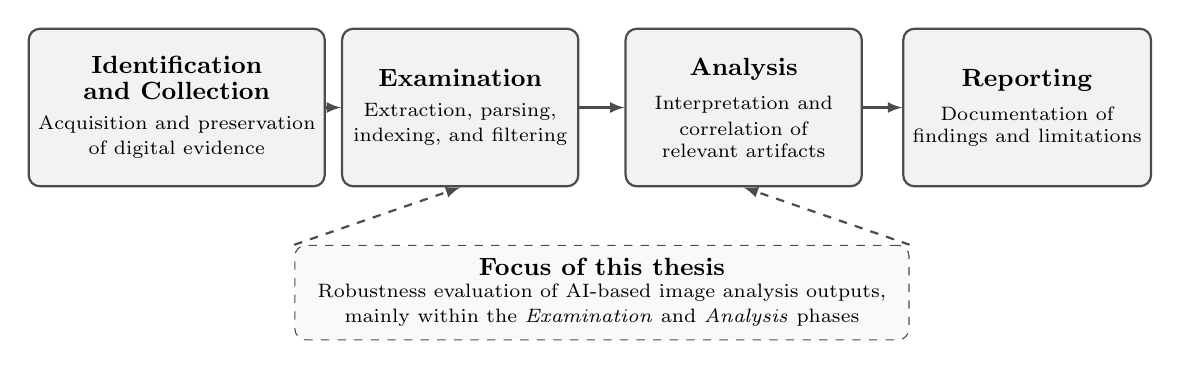
\begin{tikzpicture}[
        >=latex,
        font=\small,
        block/.style={
            rectangle,
            rounded corners,
            draw=black!70,
            thick,
            align=center,
            minimum height=2.0cm,
            minimum width=3.0cm,
            fill=gray!10
        },
        note/.style={
            rectangle,
            rounded corners,
            draw=black!70,
            dashed,
            align=center,
            minimum height=1.2cm,
            minimum width=7.8cm,
            fill=gray!5
        },
        arrow/.style={
            ->,
            thick,
            draw=black!70
        }
    ]

    \node[block] (collection) at (0,0)
    {\shortstack{
        \textbf{Identification}\\
        \textbf{and Collection}\\[1mm]
        \scriptsize Acquisition and preservation\\
        \scriptsize of digital evidence
    }};

    \node[block] (examination) at (3.6,0)
    {\shortstack{
        \textbf{Examination}\\[1mm]
        \scriptsize Extraction, parsing,\\
        \scriptsize indexing, and filtering
    }};

    \node[block] (analysis) at (7.2,0)
    {\shortstack{
        \textbf{Analysis}\\[1mm]
        \scriptsize Interpretation and\\
        \scriptsize correlation of\\
        \scriptsize relevant artifacts
    }};

    \node[block] (reporting) at (10.8,0)
    {\shortstack{
        \textbf{Reporting}\\[1mm]
        \scriptsize Documentation of\\
        \scriptsize findings and limitations
    }};

    \draw[arrow] (collection) -- (examination);
    \draw[arrow] (examination) -- (analysis);
    \draw[arrow] (analysis) -- (reporting);

    \node[note] (thesisfocus) at (5.4,-2.35)
    {\shortstack{
        \textbf{Focus of this thesis}\\
        \scriptsize Robustness evaluation of AI-based image analysis outputs,\\
        \scriptsize mainly within the \emph{Examination} and \emph{Analysis} phases
    }};

    \draw[arrow, dashed] (thesisfocus.north west) -- (examination.south);
    \draw[arrow, dashed] (thesisfocus.north east) -- (analysis.south);

    \end{tikzpicture}%
    }
    \caption{Simplified digital forensic workflow}
    \label{fig:df_workflow}
\end{figure}

% ─────────────────────────────────────────────────────────────────────────────
\subsection{Acquisition and Preservation of Digital Evidence}
\label{subsec:background_acquisition_preservation}
% ─────────────────────────────────────────────────────────────────────────────
The acquisition phase aims to make copies or extractions of digital evidence
available for examination while preserving, as far as possible, their state,
integrity, and traceability. The operational procedures depend on the nature of
the source, its state at the time of intervention, and the type of information
being sought. In general terms, a distinction can be made between the
acquisition of persistent data from storage media and the acquisition of
volatile data from active systems. In both cases, the operations performed must
be documented in a way that enables the subsequent reconstruction of the
acquisition process \cite{nist2006guide,iso27037,casey2011digital}.

In the case of storage media accessible under controlled conditions, a central
technique is physical acquisition, or \textit{bit-stream imaging}, through
which a sector-by-sector copy of the original medium is produced. Unlike a
simple logical copy of visible files, a bit-stream image may also preserve
unallocated space, \textit{slack space} areas, file system structures, and
remnants of deleted data that may be relevant to the investigation. When
technically applicable, the use of \textit{write blocking} devices makes it
possible to prevent accidental write operations on the source medium during
acquisition. The integrity of the copy is then verified through cryptographic
hash functions, such as \gls{sha256}, with the values obtained, tools used,
operators, date, and conditions of the activity documented within the chain of
custody \cite{carrier2005filesystem,iso27037,swgde_guidelines}.

Logical acquisition, by contrast, consists of extracting the data made
available by the operating system, the application, or the device under
analysis, without necessarily including the entire physical structure of the
medium. This mode may be relevant, for example, for acquiring application
content, multimedia archives, or data accessible from mobile devices and
digital services. It may allow information of interest to be obtained rapidly,
but it has limitations with respect to the completeness of the recovered data
and the availability of unallocated areas or deleted artifacts.

When the system is powered on or contains information that would be lost upon
shutdown, a \textit{live} acquisition may be necessary. This may include
volatile memory, running processes, active network connections, open sessions,
mounted encrypted volumes, or other transient elements. Live acquisition
inevitably involves interaction with the system under analysis and must
therefore be justified and documented with particular caution, specifying which
changes were introduced by the operator's activity or by the tools employed
\cite{nist2006guide,casey2011digital}.

For the purposes of this thesis, these principles are relevant because the
images subjected to automated classification must be considered digital
artifacts whose provenance, integrity, and processing history affect the
interpretation of the results. Robustness evaluation therefore does not replace
the procedures for acquiring and preserving evidence, but is situated
downstream from them, examining the reliability of automated support applied to
content that has already been acquired and organized under documented
conditions.


% ─────────────────────────────────────────────────────────────────────────────
\subsection{Examination, Analysis, and Triage of Digital Content}
\label{subsec:background_examination_analysis}
% ─────────────────────────────────────────────────────────────────────────────
Once evidence has been acquired and preserved, the \textit{examination} phase
aims to identify, extract, and organize potentially relevant artifacts. Commonly
used techniques include file system analysis, recovery of deleted files,
\textit{file carving}, metadata examination, keyword searching, content
indexing, hash-based comparison, and the extraction of artifacts generated by
operating systems or applications. These activities make it possible to reduce
the volume of raw data and isolate sets of content to be subjected to subsequent
technical and investigative assessment
\cite{carrier2005filesystem,casey2011digital,nist2006guide}.

The \textit{analysis} phase instead concerns the interpretation of the extracted
artifacts and their correlation with the investigative hypotheses. It may
include the temporal reconstruction of events through \textit{timeline
analysis}, comparison across different sources, interpretation of metadata, the
identification of relationships among files, users, or devices, and the
assessment of the investigative significance of multimedia content. In this
phase, the mere presence of a file is not sufficient: its relevance, context,
reliability, and relationship with the other available elements must be
established.

In the case of large collections of images and videos, examination and analysis
activities may be preceded or supported by triage procedures. Triage aims to
prioritize potentially relevant content without replacing the analyst's
verification. In this context, semantic search, visual grouping, and automated
classification functionalities may help highlight images compatible with
investigative categories of interest, such as the presence of a weapon.
However, the operational value of these functionalities depends on their
reliability: a false negative may reduce the likelihood that relevant content
will be examined promptly, whereas a false positive may unnecessarily increase
the review burden.

The present thesis is positioned precisely at this point in the forensic
workflow. It does not evaluate acquisition techniques or propose a method for
authenticating digital evidence, but analyzes the operational robustness of
automated classification and semantic image retrieval as forms of support for
triage and the examination of previously acquired visual content. This
distinction is methodologically essential: proper acquisition ensures
preservation of the artifact, whereas the evaluation conducted in this work
concerns the reliability of subsequent automated selection when the image is
clean, out-of-distribution, degraded, or intentionally manipulated.


% ─────────────────────────────────────────────────────────────────────────────
\section{Artificial Intelligence in Digital Forensics}
\label{sec:background_ai_digital_forensics}
% ─────────────────────────────────────────────────────────────────────────────
The integration of \gls{ai} into \gls{df} addresses the increasing
quantitative and qualitative complexity of digital investigations. The growing
volume of data acquired from personal devices, cloud infrastructures, mobile
systems, messaging applications, and multimedia archives makes an exclusively
manual analysis progressively less sustainable. In this scenario, automation
techniques, intelligent indexing, and assisted classification can support the
analyst in the preliminary selection of potentially relevant information,
reducing the operational workload and accelerating the examination and analysis
of digital evidence \cite{garfinkel2010digital,costantini2019digital}.

In forensic contexts, \gls{ai} can be employed for heterogeneous tasks,
including pattern recognition, the grouping of similar content, semantic search,
the automated classification of images and documents, anomaly detection, and
the prioritization of artifacts to be submitted to human review. These
functionalities do not replace the operator's evaluative activity, but they can
support the navigation of large datasets, especially when the evidence contains
large amounts of multimedia content or poorly structured information. The
relevance of \gls{ai} in \gls{df} should therefore be understood in terms of
investigative assistance, rather than as an automated delegation of evidentiary
decision-making \cite{costantini2019digital,faqir2023digital}.

The use of \gls{ml} and \gls{dl} models, however, introduces a discontinuity
with respect to traditional forensic tools. Many classical digital analysis
procedures rely on deterministic rules, known signatures, hashes, metadata,
keyword searches, or file system structures. Machine learning models, by
contrast, produce probabilistic outputs based on representations learned from
data. This characteristic makes it possible to process complex content, such as
images, videos, and natural language text, but it also requires closer
attention to the quality of the training data, the distribution of inputs,
model generalization, and the stability of predictions under non-ideal
conditions.

In forensic settings, this distinction is particularly relevant because the
output of an \gls{ai}-based system can influence how the analyst explores the
evidence. An incorrect classification does not necessarily determine an
autonomous evidentiary conclusion, but it may affect the priority assigned to
specific content, the visibility of relevant artifacts, or the overall
efficiency of the investigative workflow. Consequently, the reliability of an
automated module cannot be assessed solely through aggregate accuracy metrics,
but must also be considered with respect to false positives, false negatives,
distributional bias, and scenarios involving intentional manipulation.

Recent literature has shown that the use of \gls{ai}-based functionalities in
software employed for forensic analysis raises a specific validation problem:
it is not sufficient to verify that the system works correctly on ordinary
data; it is also necessary to understand its behavior in the presence of
degraded, manipulated, or out-of-distribution data
\cite{sanna2024preliminary,sanna2025pixelperfect}. This aspect is especially
important when the analysis concerns visual content, since images and videos
can be altered through compression, resizing, blurring, contrast modification,
or adversarial perturbations. Under such conditions, a system that appears
accurate on clean data may exhibit a significant reduction in its
classification capability.

For these reasons, the adoption of \gls{ai} in \gls{df} must be accompanied by
a paradigm based on human supervision, technical documentation, and experimental
evaluation of robustness. The analyst must be able to understand the role
played by the automated system, the limitations of the classification produced,
and the conditions under which the model may generate errors. From this
perspective, \gls{ai} does not represent a substitute for forensic expertise,
but rather a support tool whose usefulness depends on the possibility of
verifying its performance, stability, and reliability within the operational
context in which it is used.

The case of automated image classification constitutes a particularly
significant domain for analyzing these issues. Images may contain information
directly relevant to an investigation, but they are also subject to technical
transformations and manipulations that can modify their appearance, metadata,
or statistical characteristics. For this reason, before introducing the
principles of \gls{ml} and \gls{dl} applied to computer vision, it is necessary
to clarify the role of images as digital evidence and the meaning of their
automated classification in the context of \textit{image forensics}.


% ─────────────────────────────────────────────────────────────────────────────
\section{Image Forensics and Automated Classification}
\label{sec:background_image_forensics}
% ─────────────────────────────────────────────────────────────────────────────
Digital images represent a particularly relevant category of evidence in
contemporary forensic investigations. They may document places, objects,
persons, behaviors, tools, or circumstances that are potentially significant
for the reconstruction of an event. Unlike other digital artifacts, however,
an image combines a visual dimension that is immediately interpretable by the
human observer with a complex technical structure, consisting of pixel values,
metadata, compression parameters, information about the acquisition device, and
possible traces of subsequent processing. For this reason, forensic image
analysis requires consideration of both the depicted content and the digital
properties of the file that represents it \cite{farid2016photo,stamm2013information}.

\textit{Image forensics} focuses on the study of digital images with the aim of
assessing their origin, integrity, authenticity, and possible manipulations.
Classical techniques in this domain include, among others, metadata analysis,
the study of compression artifacts, the search for statistical inconsistencies,
the identification of resampling traces, and the examination of signals
associated with the image acquisition process. These signals include traces
produced by the photographic sensor of the acquisition device, such as the CMOS
or CCD sensor integrated into a camera or smartphone. In particular, \gls{prnu}
represents a characteristic noise component attributable to non-uniformities in
sensor response and may be used, in specific forensic analyses, to support the
attribution of an image to an acquisition device \cite{lukas2006prnu}. Such
analyses do not aim merely to establish whether an image is visually plausible,
but to verify whether the file contains technical elements compatible with a
specific origin or a specific processing history
\cite{popescu2005exposing,farid2016photo}.

In the context of the present thesis, \textit{image forensics} is considered
primarily as a conceptual framework for understanding the complexity of images
as digital evidence. The focus is not the direct detection of forgeries or
manipulations through specialized forgery detection techniques
\cite{cozzolino2017recasting}, but the evaluation of automated classification
and semantic retrieval of visual content in a forensic context. This
distinction is important: determining whether an image has been manipulated and
classifying what it represents are two different tasks, although they may
interact. A manipulation or degradation of the image may not be the primary
object of the analysis, but it may nevertheless affect the ability of an
automated tool to correctly recognize the depicted content.

Automated image classification consists of assigning an image to one or more
semantic categories on the basis of its visual content. In forensic contexts,
such categories may correspond to objects, scenes, persons, documents,
sensitive content, or elements considered relevant to an investigation. This
form of automation can support the analyst in managing large multimedia
collections, making it possible to filter, sort, or prioritize potentially
relevant images. However, automated classification must not be interpreted as
an autonomous evidentiary determination: it produces a technical indication
that requires contextualization, verification, and human supervision.

The reliability of automated classification also depends on the technical
characteristics of the image. Resolution, visual quality, illumination,
occlusions, perspective, \gls{jpeg} compression, resampling, blurring, and
color modifications can alter the digital representation of the content and
reduce the stability of predictions. Some transformations are common in normal
image production and sharing flows, for example when content is uploaded to
social platforms, forwarded through messaging applications, or saved multiple
times in compressed formats. Other transformations may instead be introduced
deliberately to degrade the image, mask details, or make automated analysis
more difficult.

This sensitivity is particularly critical in forensic contexts, because a
classification error may affect the preliminary evidence selection process. A
false negative may prevent a relevant image from being brought to the analyst's
attention, whereas a false positive may increase the review burden and generate
irrelevant investigative paths. In both cases, the problem concerns not only the
technical performance of the classifier, but also the relationship among
automation, investigative priority, and the reliability of the forensic
workflow.

Therefore, automated image classification in forensic contexts must be
evaluated by considering not only the correctness of the prediction on clean
data, but also its stability with respect to realistic conditions of
acquisition, compression, degradation, and manipulation. This aspect directly
connects \textit{image forensics} to the evaluation of the robustness of
\gls{ai}-based models. Before discussing adversarial attacks and anti-forensic
techniques, it is necessary to introduce the principles of \gls{ml} and
\gls{dl} that enable computer vision systems to learn visual representations
and produce automated classifications.


% ─────────────────────────────────────────────────────────────────────────────
\section{Machine Learning and Deep Learning for Computer Vision}
\label{sec:background_ml_dl_cv}
% ─────────────────────────────────────────────────────────────────────────────
Computer vision encompasses the set of computational methods aimed at the
automated analysis of images and videos, with the objective of extracting
structured information from visual content. In this domain, \gls{ml} and
\gls{dl} techniques have progressively replaced or complemented approaches
based on manually designed features, enabling models to learn visual
representations directly from data. In the case of image classification, the
problem consists of associating one or more semantic labels with an image on
the basis of the observable characteristics of its visual content
\cite{bishop2006pattern,gonzalez2018digital}.

Within the computer vision domain, it is useful to distinguish among related
but non-equivalent tasks. \textit{Image classification} assigns one or more
semantic labels to the entire image; \textit{object recognition} concerns the
recognition of the presence or category of an object represented in the visual
content; \textit{object detection} adds to this recognition the spatial
localization of the object, typically through regions or \textit{bounding
boxes}; finally, \textit{semantic search} enables the retrieval of images
consistent with a textual description or concept. In the present thesis, the
main experimental task is formulated as binary semantic image classification,
based on the presence or absence of firearm-related visual content of
investigative relevance, such as clearly recognizable realistic individual
firearms. Accordingly, the \texttt{weapon} class does not require the geometric
localization of the object within the image, but rather the correct
identification of the content as relevant to the forensic triage task. This
setting is consistent with studies that have applied AI-based systems to the
classification of images extracted from criminal evidence, including
operational categories such as firearms and ammunition
\cite{silva2021microservices}.

In the supervised learning paradigm, a model is trained on a set of annotated
examples, each consisting of an input and a corresponding class label. During
training, the model learns a decision function capable of associating new
inputs with one of the classes defined by the task. The objective is not to
memorize the observed examples, but to generalize correctly to unseen data.
This distinction is central in forensic contexts, because a classifier used on
real evidence may encounter images that differ from those present in the
training data in terms of quality, provenance, resolution, compression, visual
context, or semantic distribution.

The quality of generalization depends on several factors, including the
representativeness of the dataset, the consistency of the annotations, class
separability, data balance, and the model's ability to learn features that are
genuinely relevant to the task. In the absence of these conditions, a system may
achieve good performance on a controlled test set while being less reliable in
realistic scenarios. This problem is particularly relevant in forensic tasks,
where images may originate from heterogeneous sources, be degraded by
compression or sharing processes, or contain ambiguous and out-of-distribution
cases.

Traditional \gls{ml} approaches applied to image classification are often based
on a separation between feature extraction and classification. Visual features
are computed through descriptors designed or selected according to the problem,
while a classifier learns a decision rule in the feature space. Models such as
\gls{svm} have long represented an effective solution for supervised
classification problems, owing to their ability to construct robust decision
surfaces in high-dimensional spaces
\cite{cortes1995support,bishop2006pattern}. General-purpose libraries such as
scikit-learn provide standardized implementations of classical supervised-learning
algorithms and evaluation utilities, supporting reproducible experimentation
across conventional \gls{ml} workflows \cite{pedregosa2011scikit}. However, the
quality of the result depends strongly on the choice of features and on their
ability to represent image content in a discriminative manner.

\gls{dl} has profoundly changed this paradigm by introducing models capable of
automatically learning hierarchical representations of data. In \gls{cnn} architectures,
the first layers tend to capture simple visual structures, such as edges, textures, and local contrasts,
whereas deeper layers combine this information into more abstract and
semantically meaningful representations. Architectures such as ResNet have
shown the effectiveness of residual connections for training deep networks,
mitigating the degradation problem encountered during optimization and improving
the ability to learn complex visual representations \cite{he2016deep}. Later
models, such as EfficientNet, introduced more balanced scaling strategies across
depth, width, and image resolution, with the objective of improving the
relationship between performance and computational cost \cite{tan2019efficientnet}.

Alongside convolutional architectures, vision-language models capable of
learning joint representations of images and text have become increasingly
prominent in recent years. In these systems, an image is not analyzed only with
respect to predefined classes during training, but can also be associated with
textual descriptions or more general semantic concepts. Models such as
\gls{clip} have shown the possibility of learning transferable visual
representations from large-scale language supervision, opening the way to
zero-shot or text-guided classification \cite{radford2021learning}. This
approach is particularly interesting in contexts in which operational
categories do not perfectly correspond to the classes available in traditional
datasets, but it also introduces new challenges related to prompt formulation,
semantic coverage of the classes, and prediction stability.

Alongside \gls{clip}, generative vision-language models such as \gls{blip} also
make it possible to associate images with textual descriptions, introducing a
complementary perspective with respect to closed-set classification based on
predefined labels \cite{li2022blip}. In forensic contexts, such models may
support forms of automated description of visual content and contribute to the
preliminary prioritization of multimedia artifacts. However, their use requires
particular caution, because the generated description may be sensitive to image
quality, data distribution, prompt formulation, and the presence of ambiguous
or out-of-distribution content.

In the experimental protocol of the present thesis, \gls{blip} is not used as a
main proxy model. Its introduction in the background serves a contextual
function, as it helps frame the evolution of vision-language models and their
possible use in scenarios involving automated image analysis. The experimental
evaluation instead focuses on proxy models that are more directly comparable in
the binary \texttt{weapon}/\texttt{non\_weapon} task and on \gls{ai}-based
software selected for operational evaluation in a forensic context. For the
latter, analyzed in a black-box setting, the thesis does not assume any
specific internal architecture for recognition, retrieval, tagging, or object
localization, but evaluates the observable behavior of the outputs available to
the analyst, such as classifications, tags, semantic bookmarks, or
visual and semantic retrieval results, with respect to the experimental conditions
considered.


From a forensic perspective, model choice cannot be assessed exclusively as a
function of average accuracy. An automated classification system must also be
considered with respect to its behavior on heterogeneous, degraded, ambiguous,
or out-of-distribution data.

Such inputs may produce incorrect closed-set assignments or predictions
associated with high maximum predicted-class probabilities. Evaluating
\gls{ood} behavior therefore makes it possible to observe how frequently
content outside the nominal task is assigned to the known operational classes
and how the corresponding probability outputs are distributed
\cite{hendrycks2017baseline,fort2021exploring}.

These probability values remain architecture-specific and may not be
calibrated. They must therefore be interpreted as intra-model diagnostic
outputs rather than as direct measures of correctness, certainty, or forensic
reliability.

This setting motivates the introduction of a separate experimental
\gls{ood} branch, distinct from the two supervised operational classes. In the
present thesis, this branch represents borderline, anomalous, degraded,
synthetic, or otherwise out-of-task content with respect to the
\texttt{weapon}/\texttt{non\_weapon} task.

The branch is evaluated separately and is not used to train a three-class
classifier. Its inclusion also does not presuppose that the black-box software
systems implement a dedicated \gls{ood}-detection mechanism or expose an
explicit unknown state.




A further aspect concerns the probabilistic interpretation of outputs. Many
classification models produce scores or probabilities associated with classes,
but these values do not necessarily correspond to a direct measure of
evidentiary reliability. High confidence may result from spurious correlations,
dataset bias, or overfitting to the training distribution. For this reason, the
use of \gls{ml} and \gls{dl} models in a forensic workflow requires a cautious
assessment in which automated predictions are considered analytical support
rather than autonomous determinations.

Forensic computer vision must therefore confront a methodological tension: on
the one hand, \gls{dl} models make it possible to analyze large quantities of
images with performance that is often superior to traditional approaches; on
the other hand, their reliability may decrease in the presence of visual
variations, anti-forensic transformations, adversarial perturbations, or
out-of-distribution inputs. This tension justifies the need to study the
robustness of classifiers not only under clean and controlled conditions, but
also in realistic scenarios in which visual content may be degraded,
manipulated, or deliberately altered.

% ─────────────────────────────────────────────────────────────────────────────
\section{Adversarial Machine Learning}
\label{sec:background_adversarial_ml}
% ─────────────────────────────────────────────────────────────────────────────
\gls{advml} studies the behavior of machine learning systems in the presence of
inputs constructed or modified with the aim of altering their operation. Unlike
errors due to random noise, poor data quality, or generalization limits,
adversarial attacks presuppose the presence of an actor who deliberately
modifies the input in order to induce the model to produce an incorrect
prediction. In the computer vision domain, this problem is particularly
relevant because small variations in digital content may be sufficient to
change the classification produced by a model, even when the image remains
apparently similar to a human observer
\cite{szegedy2014intriguing,goodfellow2015explaining}.

An adversarial example can be described, in general terms, as an input modified
with respect to an original sample, but constructed so as to induce the
classifier to produce an incorrect label. Let \(x\) denote the original image,
\(y\) its correct class, and \(f(\cdot)\) the classifier. The attacker's
objective is to generate a perturbed version \(x'\), such that \(x'\) remains
sufficiently close to \(x\) according to a distance or perceptibility
constraint, but is classified differently by the model. In simplified form, the
problem can be expressed as the search for a perturbation \(\delta\) such that:
\[
x' = x + \delta
\quad \text{and} \quad
f(x') \neq y.
\]

The perturbation \(\delta\) is often constrained by distance metrics or
\(\ell_p\)-norm constraints, expressed as \(\|\delta\|_p \leq \epsilon\), where
\(\epsilon\) represents the maximum allowed perturbation budget and, in the most
common cases, \(p \in \{0,2,\infty\}\). These constraints make it possible to
formalize sparse attacks, limited-energy perturbations, or modifications that
are uniformly bounded across pixels, respectively, although they do not exhaust
the problem of visual perceptibility in real-world scenarios
\cite{carlini2017towards,akhtar2018threat}.

This formulation highlights the dual nature of the attack: on the one hand, the
perturbation must be limited; on the other hand, it must be sufficiently
effective to change the system's decision.

Figure~\ref{fig:adv_example} conceptually represents this mechanism in the
context of an evasion attack.

\begin{figure}[htbp]
    \centering
    \resizebox{\textwidth}{!}{%
        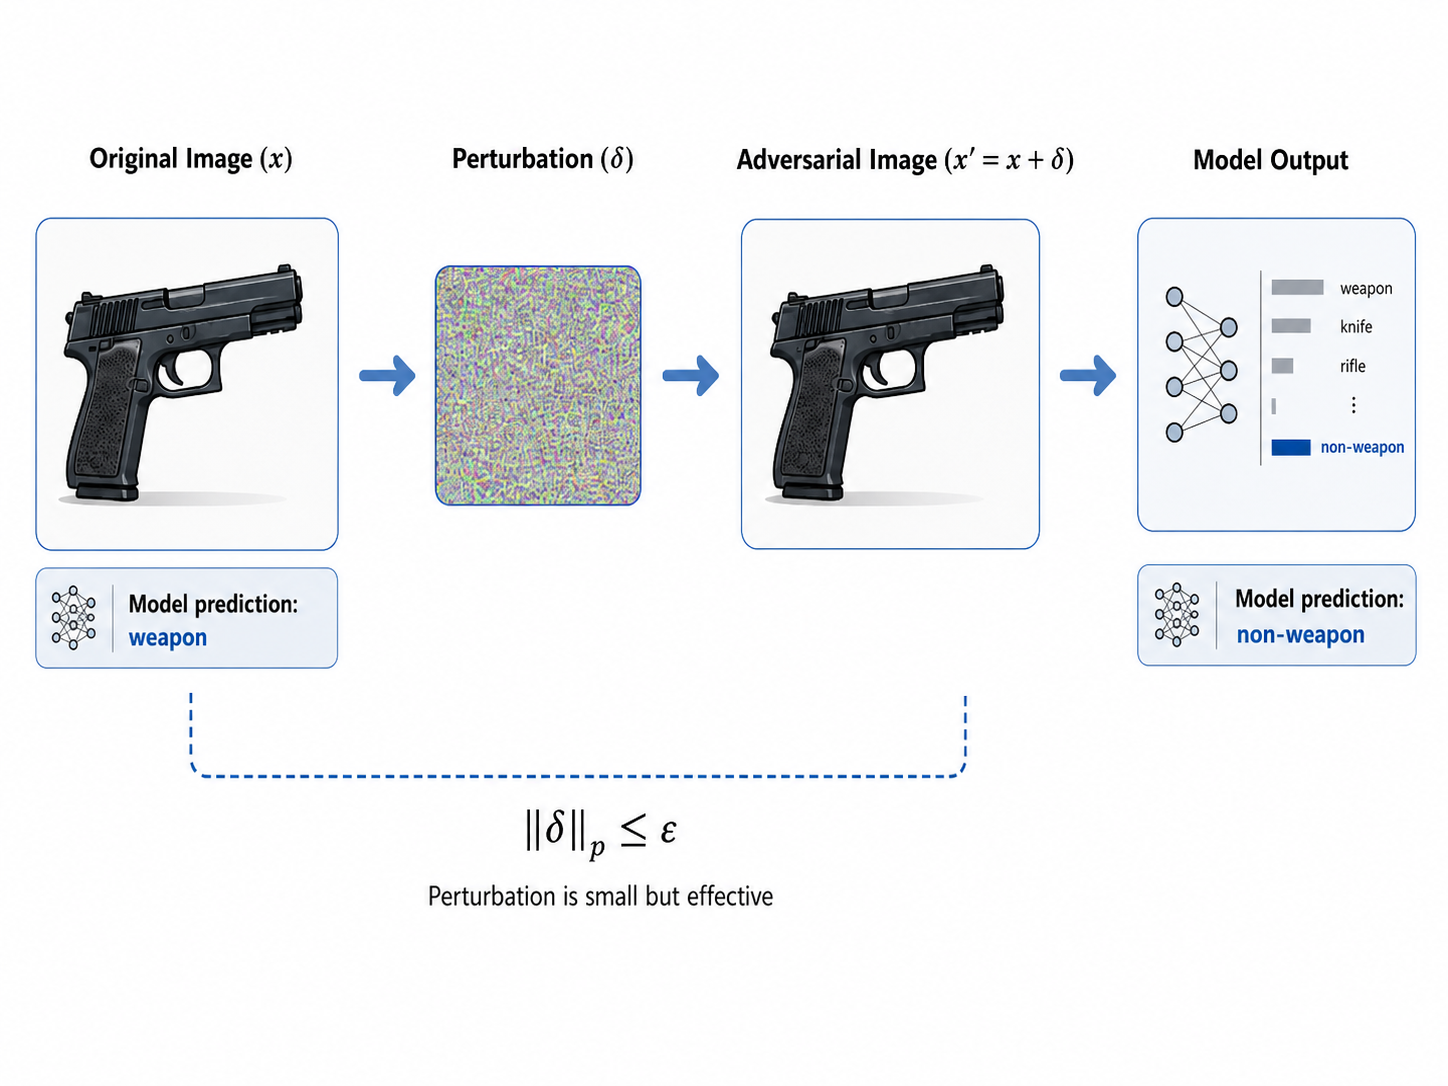
\includegraphics{images/adversarial_example_logic}
    }
\caption[Conceptual representation of an adversarial evasion attack]{Conceptual representation of an adversarial evasion attack. A bounded perturbation \(\delta\) is added to the original input \(x\) to obtain an adversarial image \(x'\), which induces a wrong classifier prediction while preserving visual coherence for a human analyst}
    \label{fig:adv_example}
\end{figure}

Adversarial attacks can be classified according to several criteria. A first
distinction concerns the phase of the model life cycle in which the attack is
conducted. Poisoning attacks occur during the training phase, by altering the
data or labels with the aim of compromising the resulting model. Evasion
attacks, by contrast, occur at inference time and consist of manipulating the
inputs submitted to an already trained model
\cite{biggio2018wild,papernot2016limitations}. In the context of automated
image classification in forensic settings, the main focus is on evasion
attacks, because the most relevant scenario is one in which images already
present on a device, in an archive, or within digital evidence are altered to
reduce the likelihood of being correctly identified by an automated tool.

A second distinction concerns the level of knowledge available to the attacker.
In white-box scenarios, the attacker has complete or extensive information
about the model, including its architecture, parameters, loss function, and
gradients. In these cases, the perturbation can be optimized directly with
respect to the internal behavior of the classifier. In black-box scenarios, by
contrast, the attacker does not know the details of the model and may rely only
on observable outputs, repeated queries, surrogate models, or the
transferability of adversarial examples across different classifiers
\cite{papernot2016limitations,carlini2017towards,yuan2019adversarial}. This
distinction is particularly important in the present thesis, because the
commercial software selected for operational evaluation is observed in a
black-box setting and does not allow assumptions about access to the parameters
or internal logic of any AI-based components.

A further distinction concerns the objective of the attack. In untargeted
attacks, the intent is simply to induce the model to produce a class different
from the correct one. In targeted attacks, by contrast, the objective is to
push the classifier toward a specific class chosen by the attacker. In the case
of forensic images, an untargeted attack may be sufficient to reduce the
ability of the tool to retrieve relevant content, whereas a targeted attack
could aim to make sensitive content appear as if it belonged to an innocuous
category. However, in an evidentiary context, even less controlled forms of
error may have significant operational consequences, because they affect the
selection, prioritization, and review of digital evidence.

The literature has proposed numerous techniques for generating adversarial
examples, differentiated by perturbation constraint, computational cost,
required knowledge, and transferability. Gradient-based methods, such as
\gls{fgsm}, exploit the information provided by the loss function to identify
an effective perturbation direction \cite{goodfellow2015explaining}. Other
approaches aim to produce more optimized, sparser, or more localized
perturbations, reducing the number of modified pixels or approximating minimal
perturbations capable of crossing the classifier's decision boundary
\cite{carlini2017towards,su2019onepixel,moosavi2016deepfool,zhang2024superdeepfool}.
In this chapter, these techniques are framed at a conceptual level; the
rationale for their selection, the adopted configurations, and the procedures
used to apply them within the experimental protocol are discussed in the
methodology chapter.

In forensic contexts, the adversarial problem does not concern only the
abstract vulnerability of models, but also their operational reliability within
an investigative process. If an \gls{ai}-based system is used to filter or
classify large quantities of images, a perturbation capable of altering its
prediction may reduce the likelihood that relevant content will be promptly
brought to the analyst's attention. The risk does not necessarily consist in
the automated production of an incorrect judicial decision, but rather in the
possibility that automation may modify the path of discovery, prioritization,
and interpretation of evidence. For this reason, adversarial robustness must be
considered a component of the broader technical-forensic reliability of the
system.

% ─────────────────────────────────────────────────────────────────────────────
\subsection{Threat Model and Attacker Assumptions}
\label{subsec:background_threat_model}
% ─────────────────────────────────────────────────────────────────────────────
The threat model defines the assumptions concerning the attacker's capabilities,
objectives, and constraints. In \gls{advml}, it is necessary to rigorously
delimit the attack scenario and to avoid robustness evaluations that lack an
operational context. Without an explicit threat model, the result of an
adversarial test risks being difficult to interpret, because it is not clear
which type of adversary the system is able to tolerate and which conditions are
instead excluded from the analysis
\cite{carlini2017towards,yuan2019adversarial}.

In the context of automated image classification in forensic settings, the
attacker can be modeled as an actor interested in reducing the likelihood that
specific content will be correctly identified by an automated tool. The main
objective is not necessarily to compromise the entire forensic workflow, but to
alter the classifier's response on specific visual inputs. In operational
terms, this may translate into the attempt to transform a relevant image into
one classified as non-relevant, ambiguous, or belonging to a category different
from the expected one. This scenario is consistent with an evasion attack,
because the manipulation affects the analyzed input rather than the model
training phase.

The attacker's capabilities may vary depending on the level of access to the
target system. In a white-box scenario, the attacker has complete or extensive
information about the model, including its architecture, parameters, loss
function, and gradients, and can therefore construct perturbations directly
optimized with respect to the classifier. In a black-box scenario, by contrast,
the attacker does not have access to the internal logic of the target system
and may rely on observable outputs, surrogate models, or the transferability of
adversarial examples. In the protocol of the present thesis, white-box access is
relevant for the controlled evaluation of proxy models when required by the
specific attack technique, whereas the selected commercial software is observed
in a black-box setting, since its internal classification logic is not
available. This distinction affects the type of attack that can be applied, the
required computational cost, and the operational plausibility of the threat.

The threat model must also specify the constraints imposed on the perturbation.
In the image domain, the modification may be limited in terms of numerical
magnitude, perceptual distance, number of altered pixels, affected image area,
or admissible transformations. In forensic contexts, these constraints acquire
a specific meaning: an excessively visible manipulation may be detected by the
human analyst or by integrity-control procedures, whereas a subtler
modification may preserve the visual plausibility of the image while still
altering the model prediction. The notion of imperceptibility must therefore be
treated with caution, because human perception, file quality, and the
investigative relevance of visual details do not necessarily coincide with a
simple mathematical distance metric.

A further aspect concerns the attacker's knowledge of the forensic domain. In
realistic scenarios, the attacker may not know the specific tool used by the
analyst, but may be aware that images and multimedia content are often subjected
to automated classification. This partial knowledge may be sufficient to
motivate transformations aimed at reducing the automatic recognizability of the
content, especially when such transformations do not clearly compromise the
general readability of the image. Therefore, the threat model must consider not
only a highly informed attacker, but also scenarios in which the adversary
operates with limited knowledge of the model and exploits generic or
transferable transformations. The operational relevance of this assumption is
consistent with the literature on adversarial examples in physical or otherwise
non-purely digital scenarios, which shows that some perturbations may retain
effectiveness even outside strictly controlled experimental conditions
\cite{kurakin2017physical}.

The threat model outlined in this subsection specifically concerns adversarial
attacks, namely perturbations constructed with the objective of altering the
classifier's response. The anti-forensic transformations discussed in the
following section instead constitute a conceptually distinct category: they may
be applied even in the absence of knowledge about the model or about any
automated classification system, and they are more generally aimed at
concealing, degrading, or making digital evidence less informative. In the
experimental protocol of the present thesis, the two categories are therefore
evaluated separately: on the one hand, adversarial perturbations oriented toward
inducing errors in the model decision; on the other hand, realistic
anti-forensic transformations not optimized with respect to the classifier,
applied to observe the stability of automated support in the presence of
plausible image manipulations. Their relationship is considered only at the
level of operational effects, since both may reduce the likelihood that
content of investigative relevance will be correctly flagged or prioritized for
subsequent analyst review.

Table~\ref{tab:threat_model} summarizes the main dimensions of the adversarial
threat model adopted in the experimental evaluation, distinguishing between the
theoretical formulation of the attacks and the operational-forensic focus of
the present thesis.

\begin{table}[htbp]
    \centering
    \small
    \renewcommand{\arraystretch}{1.25}
    \begin{tabular}{@{}p{0.24\textwidth}p{0.34\textwidth}p{0.34\textwidth}@{}}
        \toprule
        \textbf{Dimension} & \textbf{Theoretical scenarios} & \textbf{Thesis operational focus} \\
        \midrule
        \textbf{Attack phase} &
        Poisoning vs evasion &
        \textbf{Evasion}, since the manipulation affects already acquired or analyzed images at inference time. \\
        \textbf{Adversary knowledge} &
        White-box vs black-box &
        \textbf{White-box for controlled proxy-model evaluation, where required by the attack; black-box for commercial software}, whose internal \gls{ai}-based image-analysis logic is not available. \\
        \textbf{Attack objective} &
        Targeted vs untargeted &
        \textbf{Untargeted}, with emphasis on performance degradation, missed detection, and reduced classification reliability. \\
        \bottomrule
    \end{tabular}
    \caption{Adversarial threat model dimensions considered in the experimental robustness evaluation}
    \label{tab:threat_model}
\end{table}


\subsection{Adversarial and Adversarial-Style Perturbation Families}
\label{subsec:background_attack_families}

Within the general framework of \gls{advml}, this thesis considers a set of
perturbations included in the adversarial evaluation, comprising both attacks
constructed with respect to model behavior and a model-agnostic
\textit{adversarial-style} transformation. The choice is not intended to cover
the entire landscape of existing techniques exhaustively, but rather to include
perturbations that are heterogeneous in terms of computational cost, level of
knowledge required about the model architecture, alteration constraint, and
operational plausibility. In particular, gradient-based, sparse, iterative, and
model-agnostic perturbations are considered, in order to observe the behavior
of AI-based systems with respect to manipulations characterized by different
properties.

The \textbf{\acrfull{fgsm}} represents a simple and efficient adversarial
baseline. Given a classifier \(f\), a loss function \(\mathcal{L}\), an image
\(x\), and the corresponding correct label \(y\), the attack generates a
perturbed image by moving in the direction of the sign of the gradient of the
loss with respect to the input:
\[
x' = x + \epsilon \cdot \operatorname{sign}
\left(\nabla_x \mathcal{L}(f(x), y)\right).
\]
The parameter \(\epsilon\) controls the maximum magnitude of the perturbation.
In the experimental context of the thesis, \gls{fgsm} is relevant because it
makes it possible to rapidly evaluate the classifier's sensitivity to a
single-step white-box perturbation constructed directly with respect to the
model's loss function \cite{goodfellow2015explaining}.

The \textbf{\gls{onepixel}} instead represents a family of sparse and black-box
attacks, in which the perturbation is constrained to modify a very limited
number of pixels. In general form, the objective is to find a version \(x'\) of
the image such that:
\[
f(x') \neq f(x)
\quad \text{with} \quad
\|x - x'\|_0 \leq k,
\]
where \(k\) denotes the maximum number of pixels that can be modified. In the
extreme case of the \gls{onepixel}, \(k=1\). The attack is relevant because it
shows how highly localized variations can alter the decision of a neural
network, even without direct access to the model gradients
\cite{su2019onepixel}.

\textbf{\gls{sigmazero}} belongs to the family of attacks oriented toward
sparsity and the \(L_0\) norm. Unlike attacks that limit the global magnitude
of the perturbation through \(L_2\) or \(L_\infty\) norms, \(L_0\) attacks aim
to reduce the number of modified input components. The objective can be
expressed as the search for an adversarial image \(x^{adv}\) such that:
\[
f(x^{adv}) \neq f(x)
\quad \text{while minimizing} \quad
\|x - x^{adv}\|_0.
\]
This setting is particularly significant in forensic contexts because sparse
perturbations may be difficult to identify through ordinary visual inspection
and may not visibly degrade the perceptual quality of the image
\cite{zhao2024sigmazero}.

\textbf{\gls{superdeepfool}} is regarded as an iterative attack inspired by
the DeepFool family. The general idea behind DeepFool is to iteratively
estimate a perturbation capable of crossing the classifier's decision boundary,
seeking a modification of limited magnitude that is sufficient to change the
model's prediction. In abstract form, the objective is to find a perturbation
\(\delta\) such that:
\[
x' = x + \delta
\quad \text{and} \quad
f(x') \neq f(x),
\]
with \(\delta\) constructed through successive updates guided by the local
geometry of the decision function. In the context of the thesis, this family of
attacks is relevant because it represents iterative perturbations that are more
structured than a single-step attack such as \gls{fgsm}, without attributing to
the technique any general ability to overcome every possible defense or form of
pre-processing \cite{moosavi2016deepfool,zhang2024superdeepfool}. This caution
is consistent with the literature showing that some defenses may produce only
apparent robustness, for example through gradient masking or obfuscated
gradients, without ensuring genuine resistance to adaptive attacks
\cite{athalye2018obfuscated}.

A further attack frequently used in the evaluation of adversarial robustness is
\gls{pgd}, which extends the idea of gradient-based attacks through iterative
updates constrained within a perturbation neighborhood and has been widely used
as a reference for formulating adversarial robustness as a model security
problem \cite{madry2018towards}. In the present thesis, however, \gls{pgd} is
not included in the main experimental protocol. This choice stems from the need
to keep the workflow computationally sustainable and focused on operational
robustness in forensic contexts, using \gls{superdeepfool} and \gls{sigmazero}
as representatives of iterative and sparse perturbations, respectively, in line
with the objectives of the experimental protocol.

Alongside attacks constructed with respect to model behavior, the thesis also
considers a model-agnostic perturbation based on shifting color channels.
\textbf{\gls{colorshift}} globally modifies the chromatic representation of the
image, for example through offsets or multiplicative factors applied to the
\(R\), \(G\), and \(B\) channels. It represents an intermediate case with
respect to the classical distinction between model-dependent adversarial attacks
and anti-forensic transformations. In this thesis, it is treated as a
model-agnostic \textit{adversarial-style} perturbation: it does not use
gradient information and does not directly optimize a model loss function, but
it is applied with the experimental purpose of evaluating the effect of
semantically conservative alterations on automated classification. For this
reason, although it shares some visual characteristics with realistic image
transformations, it is kept within the experimental group of adversarial
perturbations, explicitly qualifying it as a model-agnostic
\textit{adversarial-style} transformation and not as an attack optimized with
respect to the model.

Table~\ref{tab:background_attack_families} summarizes the adversarial and
\textit{adversarial-style} perturbations considered in the experimental
protocol.

\begin{table}[htbp]
    \centering
    \small
    \renewcommand{\arraystretch}{1.25}
    \begin{tabularx}{\textwidth}{@{}l l X@{}}
        \toprule
        \textbf{Technique} & \textbf{Family} & \textbf{Methodological relevance} \\
        \midrule
        \gls{fgsm} &
        Gradient-based, single-step &
        Efficient white-box baseline for evaluating the model's sensitivity
        to the gradient of the loss function. \\
        \gls{onepixel} &
        Sparse, black-box &
        Highly localized perturbation, useful for evaluating vulnerability to
        minimal modifications in the pixel domain. \\
        \gls{sigmazero} &
        Sparse, \(L_0\)-oriented &
        Attack oriented toward minimizing the number of modified pixels,
        relevant to scenarios in which the perturbation must remain localized. \\
        \gls{superdeepfool} &
        Iterative boundary-based &
        Iterative attack inspired by DeepFool, useful for exploring decision
        stability with respect to crossing the decision boundary. \\
        \gls{colorshift} &
        Adversarial-style, model-agnostic &
        Semantically conservative global chromatic alteration, not optimized
        with respect to the model, included among adversarial perturbations to
        evaluate the effect of controlled color variations on automated
        outputs. \\
        \bottomrule
    \end{tabularx}
    \caption{Adversarial and adversarial-style perturbations considered in the experimental protocol}
    \label{tab:background_attack_families}
\end{table}



% ─────────────────────────────────────────────────────────────────────────────
\section{Anti-Forensic Techniques Applied to Digital Images}
\label{sec:background_antiforensics_images}
% ─────────────────────────────────────────────────────────────────────────────
Anti-forensic techniques comprise the set of strategies aimed at hindering,
degrading, or making the forensic analysis of digital content less reliable. In
the image domain, such techniques may affect both the visual properties of the
content and the statistical and structural characteristics of the file, with
the objective of reducing the possibility of reconstructing the image history,
detecting manipulations, identifying acquisition traces, or correctly
classifying the depicted content. In general terms, anti-forensics does not
necessarily coincide with the explicit forgery of an image, but also includes
transformations capable of altering or masking information relevant to
technical analysis \cite{stamm2010anti,yaacoub2021digital}.

In the context of \textit{image forensics}, many analyses rely on the presence
of statistical and structural traces associated with the formation or
subsequent processing of the image file. Such traces may include compression
artifacts, patterns introduced by resampling operations, inconsistencies among
image regions, and signals attributable to the acquisition device, such as the
\gls{prnu} of the photographic sensor. Anti-forensic transformations may aim to
reduce the visibility or reliability of these indicators, making it more
difficult to distinguish between original, degraded, or manipulated content.
For example, \gls{jpeg} recompression may modify the artifacts produced by
previous saving operations; resampling may alter the spatial correlations
introduced by resizing operations; histogram or contrast modifications may
change the distribution of image intensity values
\cite{popescu2005exposing,farid2016photo,lukas2006prnu}.

In the present thesis, these techniques are discussed to frame the domain of
\textit{image forensics} and the possible manipulations of visual evidence; the
experimental evaluation does not concern source attribution through
\gls{prnu}, but rather the stability of semantic image classification with
respect to selected transformations applied in a controlled manner.

A first family of transformations concerns compression and recompression. The
\gls{jpeg} format, widely used in digital devices and sharing platforms,
applies lossy compression that modifies the frequency components of the image
and introduces artifacts depending on the selected quality level. From a
forensic perspective, such artifacts may be informative, but they may also
interfere with subsequent analyses. Intentional recompression may attenuate or
overwrite previous traces, reduce perceptual quality, or modify statistical
characteristics exploited by automated tools. For this reason, compression is
not only a normal technical step in image management, but may also become a
relevant transformation from an anti-forensic standpoint
\cite{stamm2010anti,stamm2013information}.

A second category includes geometric and resampling operations, such as
resizing, cropping, rotation, and resampling. These transformations may be
common in ordinary image production and sharing workflows, but they may also be
used to modify the scale of objects, remove relevant regions, alter scene
composition, or introduce statistical patterns different from the original
ones. Resampling, in particular, may leave traces detectable through forensic
analysis, but it may also be combined with additional transformations to make
its identification more difficult \cite{popescu2005exposing,farid2016photo}.

Additional anti-forensic transformations concern controlled visual degradation.
Blurring, noise, resolution reduction, sharpness alteration, and color
modifications may decrease the readability of relevant details without
necessarily making the image unusable for a human observer. In an
\gls{ai}-assisted forensic workflow, these transformations are particularly
important because they may modify the visual features used by classifiers. An
object that remains recognizable to the analyst may become less discriminative
for the model, especially if the transformation alters edges, textures, local
contrasts, or spatial relationships among the components of the scene.

Alongside visible or statistically detectable transformations, a further
category of techniques attributable to the anti-forensic domain concerns
steganography, namely the concealment of information within digital content. In
the case of images, additional data may be embedded by altering poorly
perceptible portions of the representation, such as the least significant bits
of pixel values. Although steganography has different purposes from visual
degradation or recompression, it is relevant within the framework of
\textit{image forensics} because it may introduce hidden content, modify the
statistical properties of the file, and require specialized analyses to
distinguish between an apparently ordinary image and an image used as a
concealment vector \cite{stamm2013information,yaacoub2021digital}.

In the present work, steganography is mentioned as a broader component of the
anti-forensic domain, whereas the experimental evaluation focuses on visual and
statistical transformations directly relevant to the robustness of automated
classification.

It is important to distinguish anti-forensic techniques from the adversarial
attacks discussed in the previous section. Adversarial attacks are generally
designed with respect to the behavior of a model and aim to induce an incorrect
prediction through optimized perturbations. Anti-forensic transformations, by
contrast, may be model-independent and more generally oriented toward
degrading, masking, or altering digital evidence. This distinction does not
imply an absolute separation: an anti-forensic transformation may produce
adversarial effects on a classifier, just as an adversarial perturbation may
have anti-forensic consequences when it reduces the investigative usefulness of
an image. However, from a methodological standpoint, the two categories must be
kept distinct because they presuppose different attacker capabilities,
objectives, and assumptions.

In the case of automated image classification, anti-forensic techniques are
relevant because they may affect the operational robustness of \gls{ai}-based
systems even in the absence of an attack optimized against the model. A
recompressed, resized, blurred, or contrast-altered image may represent a
realistic input, compatible with ordinary acquisition, storage, or sharing
processes. However, the same transformations may be intentionally exploited to
reduce the likelihood that content will be correctly classified. The difficulty
therefore lies in distinguishing between ordinary degradations within the
digital image life cycle and transformations applied with the purpose of
concealment or reduction of analytical effectiveness.

From a forensic perspective, this ambiguity requires cautious evaluation. Not
every compressed, resized, or degraded image can be considered the result of
anti-forensic conduct; on the contrary, many transformations are ordinary
consequences of the use of mobile devices, social networks, messaging
applications, and storage systems. However, when the objective is to evaluate
the reliability of automated tools, it is necessary to include such
transformations within the space of realistic scenarios. The robustness of a
forensic classifier depends not only on its accuracy on clean images, but also
on its ability to maintain stable behavior in the presence of plausible,
intentional, or accidental degradations.

From this perspective, anti-forensic techniques applied to digital images
constitute a bridge between traditional \textit{image forensics} and the
evaluation of the robustness of computer vision models. They highlight that an
image is not a static and neutral input, but a digital artifact subject to
technical transformations that may affect both its human interpretability and
its automated processing. For this reason, the evaluation of \gls{ai}-based
models and software employed in the context of \gls{df} must consider not only
formally defined adversarial attacks, but also manipulations and degradations
compatible with realistic operational scenarios.



% ─────────────────────────────────────────────────────────────────────────────
\subsection{Image-Level Anti-Forensic Transformation Families}
\label{subsec:background_antiforensic_transformations}
% ─────────────────────────────────────────────────────────────────────────────
In the context of the present thesis, anti-forensic transformations are
considered as realistic manipulations of the image artifact, not necessarily
optimized with respect to a specific classifier. They act on the visual,
statistical, or geometric properties of the file and may derive both from
ordinary acquisition, saving, and sharing processes and from intentional
applications aimed at reducing the effectiveness of automated analysis. For
this reason, such transformations constitute a bridge between traditional
\textit{image forensics} and the evaluation of the operational robustness of
\gls{ai}-based systems.

The \textbf{\gls{jpegrecompression}} transformation consists of saving an image
again using lossy compression. Since the \gls{jpeg} format operates on the
frequency components of the image and introduces artifacts depending on the
selected quality level, recompression may modify or overwrite previous traces,
alter local statistics, and degrade visual details relevant to classifiers.
From a forensic perspective, this transformation is relevant because it may
interfere both with analyses based on compression artifacts and with
\gls{ai}-based models that are sensitive to textures, edges, and local patterns
\cite{stamm2010anti,stamm2013information}.

The \textbf{\gls{resampleresize}} transformation modifies the resolution and
spatial grid of the image. Let \(x\) denote the original image. A resizing
transformation can be modeled as:
\[
x' = \mathcal{R}(x; s, \mathcal{I}),
\]
where \(s\) is the scaling factor and \(\mathcal{I}\) represents the
interpolation method. When an image is reduced and subsequently restored to its
original size, part of the spatial information is lost and replaced by
interpolated values. This process may alter pixel correlations, geometric
traces, and local patterns used by both forensic tools and classification
models \cite{popescu2005exposing,farid2016photo}.

The \textbf{\gls{gaussianblur}} transformation introduces controlled blurring
through convolution with a Gaussian kernel. In simplified form, the operation
can be described as:
\[
x' = x * G_{\sigma},
\]
where \(G_{\sigma}\) is a two-dimensional Gaussian function and \(*\) denotes
convolution. This transformation attenuates high frequencies, reduces edge
sharpness, and may decrease the discriminative value of local details. In the
context of automated classification, blur is relevant because many \gls{cnn}
models learn features in the first convolutional layers that are strongly
related to edges, textures, and local intensity variations.

The \textbf{\gls{histogrammodification}} transformation acts on the distribution
of image intensity values. In the case of \textit{histogram equalization}, the
objective is to remap intensity levels using the cumulative distribution
function, according to a transformation of the following form:
\[
x'_i = \left\lfloor (L-1)\cdot \operatorname{CDF}(x_i) \right\rfloor,
\]
where \(L\) denotes the number of intensity levels and \(\operatorname{CDF}\) is
the normalized cumulative distribution. This transformation may improve
perceived contrast, but it may also modify global and local statistics used by
image forensics tools and automated classifiers \cite{barni2018cf}.

The \textbf{\gls{contraststretching}} transformation applies a linear
normalization of the dynamic range. Let \(I_{\min}\) and \(I_{\max}\) denote two
intensity bounds, possibly computed through percentiles to reduce the influence
of outliers. The transformation can be expressed as:
\[
x'_i =
\begin{cases}
0, & \text{if } x_i \leq I_{\min}, \\
255, & \text{if } x_i \geq I_{\max}, \\
\dfrac{x_i - I_{\min}}{I_{\max} - I_{\min}} \cdot 255, & \text{otherwise}.
\end{cases}
\]
This operation modifies the global contrast of the image and may alter the
response of models with respect to dark regions, overexposed areas, or regions
with low tonal separation.

Table~\ref{tab:background_antiforensic_transformations} summarizes the
anti-forensic transformations considered in the experimental protocol.

\begin{table}[htbp]
    \centering
    \small
    \renewcommand{\arraystretch}{1.25}
    \begin{tabularx}{\textwidth}{@{}lX@{}}
        \toprule
        \textbf{Transformation} & \textbf{Methodological relevance} \\
        \midrule
        \gls{jpegrecompression} &
        Modifies compression artifacts, frequency components, and local image
        details. \\
        \gls{resampleresize} &
        Alters the spatial grid, introduces interpolation, and may degrade
        geometric correlations and local patterns. \\
        \gls{gaussianblur} &
        Attenuates high frequencies, edges, and textures, reducing the
        discriminative value of potentially relevant details. \\
        \gls{histogrammodification} &
        Remaps the distribution of intensity levels, modifying global and local
        image statistics. \\
        \gls{contraststretching} &
        Normalizes the dynamic range and alters global contrast, with possible
        effects on the features learned by classifiers. \\
        \bottomrule
    \end{tabularx}
    \caption{Anti-forensic transformations considered in the experimental protocol}
    \label{tab:background_antiforensic_transformations}
\end{table}

Table~\ref{tab:adv_vs_antiforensics} summarizes the conceptual distinction
between \textit{adversarial attacks} and \textit{anti-forensic transformations}
in the context of automated image classification.

\begin{table}[htbp]
    \centering
    \small
    \renewcommand{\arraystretch}{1.25}
    \begin{tabular}{@{}p{0.22\textwidth}p{0.34\textwidth}p{0.34\textwidth}@{}}
        \toprule
        \textbf{Dimension} & \textbf{Adversarial attacks} & \textbf{Anti-forensic transformations} \\
        \midrule
        \textbf{Primary target} &
        Decision function of the \gls{ai}-based model. &
        Visual, statistical, or structural properties of the digital image file. \\
        \textbf{Nature} &
        Perturbations designed to alter the model prediction. &
        Manipulations or degradations such as \gls{jpeg} recompression, resizing, blur, or contrast modification. \\
        \textbf{Model dependency} &
        Usually direct or surrogate-based, especially in white-box or transfer-based settings. &
        Usually low or indirect, since the transformation can often be applied without knowing the classifier. \\
        \textbf{Visibility} &
        Often designed to be imperceptible, sparse, or localized. &
        Often compatible with visible degradations or ordinary image processing operations. \\
        \textbf{Forensic relevance} &
        May affect automated evidence selection by inducing false positives or false negatives. &
        May alter the evidentiary quality of the image and reduce the reliability of automated analysis. \\
        \bottomrule
    \end{tabular}
    \caption{Comparison between adversarial attacks and anti-forensic transformations in the context of automated image classification}
    \label{tab:adv_vs_antiforensics}
\end{table}

% ─────────────────────────────────────────────────────────────────────────────
\section{Explainability, Robustness, and Model Reliability}
\label{sec:background_xai_robustness}
% ─────────────────────────────────────────────────────────────────────────────

The evaluation of an \gls{ai}-based model cannot be reduced exclusively to the
measurement of its average accuracy. In a forensic context, the usefulness of an
automated system also depends on the stability of its predictions, its ability
to handle degraded or out-of-distribution inputs, the transparency of the
information provided to the analyst, and the possibility of documenting, in a
verifiable manner, the role played by the model within the investigative
workflow. Accuracy, robustness, interpretability, and reliability are therefore
complementary dimensions that must be considered jointly when an automated
classification system is used to support the analysis of digital evidence
\cite{Adadi2018,Doshi-Velez2017}.

Robustness can be defined, in general terms, as the ability of a model to
maintain stable and coherent behavior in the presence of input variations. Such
variations may be accidental, such as noise, compression, low resolution, or
non-ideal acquisition conditions, or intentional, such as adversarial
perturbations and anti-forensic transformations. In the computer vision domain,
robustness does not concern only resistance to small numerical perturbations,
but also the classifier's ability to handle realistic changes in the visual
properties of the image, the data distribution, and the quality of the analyzed
content \cite{hendrycks2019benchmarking,ford2019adversarial}.

Reliability is a broader concept than robustness. A model may be robust with
respect to a specific family of perturbations, but not necessarily reliable in a
forensic sense. Reliability requires the system to produce results that are
sufficiently stable, verifiably documented, and interpretable with respect to the
context of use. In particular, a classifier employed in a \gls{df} workflow must
be evaluated with respect to its ability to support the analyst without
replacing human judgment, to signal uncertainty or ambiguous cases, to avoid
overestimating its own confidence, and to maintain coherent performance even on
data different from those observed during training. This distinction is
essential because an output that is formally correct on average may still be
unreliable if it is not stable, verifiable, or adequately contextualized.

The role of \gls{xai} is situated within this framework. Explainability
techniques aim to provide tools for making model behavior more understandable,
especially when models operate as complex or partially opaque systems. In
computer vision, these techniques may include saliency maps, attribution
methods, visualizations of the image regions that most influence the prediction,
and local explanations of classifier behavior. Well-known examples include
model-agnostic approaches, such as LIME and SHAP, and attribution or visual
localization techniques, such as \gls{ig} and class activation mapping
\cite{Ribeiro2016,Lundberg2017,Sundararajan2017,Zhou2016}.

These approaches are not methodologically equivalent. Gradient-based
techniques, such as \gls{ig}, require access to the model and to the gradient of
the prediction with respect to the input, and are therefore applicable to the
controllable proxy models considered in the present thesis. Model-agnostic
approaches, such as LIME or some formulations of SHAP, can instead operate
through input-output queries, but their application to commercial software
evaluated in a \textit{black-box} setting depends on the availability of
adequate outputs, queryable interfaces, and reproducible experimental
conditions. For this reason, the operational choice of the explainability
technique used in the protocol is described in Chapter~\ref{chap:methodology}.

In the case of commercial black-box software, outputs such as tags,
classifications, retrieval results, or semantic bookmarks must therefore be
interpreted as observable operational signals rather than as local explanations
of the internal decision-making process. They can be normalized and evaluated
against the experimental ground truth, but they do not make it possible to
directly infer which features, image regions, or internal representations
determined the system's decision.

The use of \gls{xai} in forensic contexts must nevertheless be interpreted with
caution. A visual explanation does not constitute autonomous proof of the
correctness of the model, nor does it guarantee that the classifier has learned
concepts that are semantically coherent with human reasoning. Saliency maps,
for example, may indicate image regions relevant to the prediction, but they do
not necessarily demonstrate that the model recognized the object of interest in
the expected way. Moreover, explanations generated by different methods may
diverge from one another, and their stability may be influenced by input
perturbations or model variations \cite{Adadi2018,Carvalho2019}.

Despite these limitations, \gls{xai} can provide useful support in the
evaluation of operational robustness. Comparing explanations produced on clean
and manipulated images may help identify variations in model behavior, shifts
in attribution toward irrelevant regions, or dependence on visual artifacts
that are not relevant to the task. In this sense, explainability should not be
understood as a conclusive validation tool, but as an auxiliary component of
the analysis, useful for formulating hypotheses about classifier behavior and
documenting possible anomalies in the system's response.

The relationship between robustness and explainability is particularly
important in cases in which a model preserves the same label but changes the
apparent rationale of the prediction, or produces an incorrect classification
while focusing on irrelevant visual regions. Such situations show that accuracy
alone is not sufficient to understand system behavior. In a forensic context,
the possibility of observing how the model reacts to degradations,
anti-forensic transformations, or adversarial perturbations can contribute to a
more complete assessment of its reliability, especially when the automated
output is used to filter or prioritize large quantities of images.

A further element concerns confidence calibration. \gls{dl} models may produce
predictions with high scores even in the presence of ambiguous, degraded, or
out-of-distribution inputs. This phenomenon is problematic in \gls{ai}-assisted
workflows, because apparently high confidence may lead the user to overestimate
the reliability of the output. Operational robustness therefore requires not
only that the model maintain good performance on manipulated data, but also
that uncertainty be handled in a coherent and non-misleading manner, especially
in cases in which the image does not clearly belong to the classes expected by
the system \cite{hendrycks2017baseline,fort2021exploring}.

Within the framework of the present thesis, explainability, robustness, and
reliability are considered complementary dimensions in the evaluation of proxy
models and in the interpretation, to the extent observable, of the outputs
produced by \gls{ai}-based software employed in the forensic context.
Robustness makes it possible to measure the stability of predictions with
respect to adversarial perturbations and anti-forensic transformations;
\gls{xai}, applied to proxy models, makes it possible to observe, with due
caution, local attributions associated with predictions; reliability integrates
these elements within the operational context, considering the role of the
analyst, the documentability of the process, and the possible consequences of
automated errors in evidence selection. This setting makes it possible to move
beyond a purely performance-based evaluation and to situate model behavior
within the verifiability requirements that characterize \gls{df}.

% ─────────────────────────────────────────────────────────────────────────────
\section{Legal and Regulatory Profiles of AI in Forensic Contexts}
\label{sec:background_legal_profiles}
% ─────────────────────────────────────────────────────────────────────────────
The use of \gls{ai} in forensic contexts raises not only technical issues, but
also affects the assumptions of reliability, verifiability, and control that
characterize digital evidence. In investigative and judicial proceedings, an
automated system may contribute to the selection, classification, or
prioritization of relevant content, but it cannot replace the assessment of the
forensic operator or that of the judicial authority. The legal dimension of
\gls{ai} in \gls{df} must therefore be traced back to the principle that any
technical result used for evidentiary purposes must be documented,
contextualized, and, as far as possible, verified through transparent and
repeatable procedures \cite{casey2011digital,iso27037,biasiotti2018handling}.

The framework of digital evidence is also situated within a supranational
regulatory context in which cybercrime and attacks against information systems
are governed by instruments such as the Budapest Convention on Cybercrime and
Directive 2013/40/EU, which reinforce the centrality of digital evidence in
investigative activities and judicial cooperation
\cite{budapest2001convention,directive2013cyber}.

Digital evidence is characterized by particular vulnerability to modification,
loss of context, and attribution difficulties. For this reason, international
standards and guidelines emphasize the need to preserve integrity,
authenticity, traceability, and the chain of custody throughout the entire
evidence management life cycle \cite{iso27037,enfsi2022}. When analysis is
supported by \gls{ai}-based modules, these requirements do not disappear;
rather, they also extend to the functioning of the automated tool. It therefore
becomes necessary to document not only the origin and handling of the data, but
also the role played by the model, the conditions of use, the available
metrics, the known limitations, and any human intervention in the assessment of
the result.

From this perspective, case law from the Court of Cassation has progressively
emphasized the need for seizure and acquisition activities involving computer
data to be supported by adequate reasoning, by criteria of relevance with
respect to the object of the investigation, and by safeguards suitable for
avoiding acquisitions or retentions that are disproportionate to evidentiary
purposes \cite{cassazione2020,cassazione2025}.

In the context of criminal investigations conducted by competent authorities,
the specific European framework on personal data protection is represented by
Directive (EU) 2016/680, transposed into the Italian legal system by
Legislative Decree No.~51 of May 18, 2018. This legal framework concerns
processing carried out for the purposes of the prevention, investigation,
detection, or prosecution of criminal offenses or the execution of criminal
penalties, including automated processing of personal data. In this context,
the use of \gls{ai}-based systems to support forensic analysis must be assessed with
respect to the principles of lawfulness, necessity, proportionality, and
security of processing, as well as the requirements of documentation and
control of the operations performed. The \gls{gdpr} remains relevant for
processing operations that do not fall within the specific scope of
\textit{law enforcement} activities, for example where similar systems are used
by private entities or in different organizational and application contexts not
attributable to the purposes of prevention, investigation, detection, or
prosecution of criminal offenses. Therefore, references to automated
decision-making and impact assessments must be applied according to the
specific legal basis and purpose of the processing
\cite{directive2016led,dlgs2018_51,gdpr2016}.

A further reference is the AI Act, which introduces a risk-based regulatory
model and pays particular attention to systems used in sensitive contexts,
including \textit{law enforcement} activities and the administration of
justice. In these areas, the use of \gls{ai} may affect fundamental rights,
procedural guarantees, and the ability of the parties to understand or contest
the outcome of an assisted decision-making process. For this reason, systems
classified as high-risk are subject to requirements concerning data governance,
technical documentation, logging, transparency, human oversight, accuracy,
robustness, and cybersecurity \cite{aiact2024}. These requirements are
particularly consistent with the needs of \gls{df}, in which every relevant
step must be reconstructable and justifiable.

However, the concrete regulatory classification of the software considered in
the present thesis depends on its intended purpose, the role actually played
within the investigative workflow, and the specific conditions of use; this
work does not automatically assume that the evaluated systems fall within a
specific risk category under the AI Act.

In the specific context of automated image classification, the legal issue does
not necessarily consist in the model producing a final decision on the
evidentiary value of the image. More realistically, the risk concerns the
indirect influence of automation on the investigative path: a false negative
may reduce the likelihood that a relevant image will be examined promptly,
whereas a false positive may direct the analyst's attention toward irrelevant
content. In both cases, the output of the automated system may affect evidence
selection and prioritization, even though it does not formally constitute a
judicial decision. This makes it necessary to adopt a cautious approach, in
which automated classification is regarded as a support tool rather than an
autonomous source of assessment.

Human oversight therefore represents a central requirement. It should not be
understood as a merely formal control, but as the actual possibility for the
operator to understand the role of the system, assess its output, recognize
conditions of uncertainty, and intervene when the automated result appears
incoherent or insufficiently reliable. In forensic contexts, oversight also has
a documentary function: the analyst must be able to explain whether and how the
model output contributed to evidence selection, which checks were performed,
and which limitations were considered in the overall assessment.

The opacity of \gls{dl} models introduces further challenges. If a system
produces a classification without making the technical reasons for the
prediction understandable, the ability to challenge, replicate, or critically
evaluate the result may be reduced. \gls{xai} techniques can partially mitigate
this problem by providing indications about the image regions or features that
most influenced the prediction. However, as discussed in the previous section,
such explanations must not be confused with proof of the model's correctness.
They constitute interpretive support tools, useful for documentation and
review, but they do not replace technical validation or human judgment
\cite{Adadi2018,Doshi-Velez2017}.

In light of these considerations, the robustness of \gls{ai}-based systems also
has legal relevance, not only technical relevance. A model vulnerable to
adversarial perturbations, realistic degradations, or anti-forensic
transformations may compromise the quality of the support provided to the
analyst and reduce the reliability of the investigative workflow. Experimental
robustness evaluation therefore helps clarify the limits within which an
automated system may be used responsibly, the conditions that may generate
errors, and the safeguards that should accompany its use in forensic scenarios.

In conclusion, the use of \gls{ai} in \gls{df} requires a balance between
operational efficiency and procedural safeguards. Automation may improve the
ability to analyze large quantities of data, but it must be integrated into a
controlled, documented, and supervised process. In the case of automated image
classification, this balance requires the model to be evaluated not only with
respect to its accuracy on clean data, but also with respect to its robustness,
explainability, traceability, and ability to operate under realistic
conditions. These elements constitute the theoretical basis for the
experimental methodology developed in the following chapters.

% ----------------- Chapter 3: State of the Art ----------------------
% ─────────────────────────────────────────────────────────────────────────────
\chapter{State of the Art}
\label{chap:state-of-the-art}
% ─────────────────────────────────────────────────────────────────────────────
This chapter examines the scientific literature relevant to the thematic axes
of the thesis, following the editorial distinction established with respect to
Chapter~\ref{chap:background}: for each area, it discusses the main existing
contributions, what they have demonstrated, and which limitations remain open,
without redefining concepts already introduced in the theoretical background.
The objective is to identify the specific gap that motivates the experimental
approach of the thesis: the limited availability, in the existing literature,
of integrated experimental protocols for evaluating the operational robustness
of proxy models and AI-based software in realistic forensic scenarios.


% ─────────────────────────────────────────────────────────────────────────────
\section{AI and Automation in Digital Forensics}
\label{sec:sota-ai-df}
% ─────────────────────────────────────────────────────────────────────────────

The scale of digital data represents the starting point of the literature on
automation in \gls{df}. Garfinkel~\cite{garfinkel2010digital}, in a work that
shaped research over the following decade, documented how the rapid growth of
digital data volumes was making manual analysis increasingly unsustainable,
identifying automation as one of the priority directions for investment. The
contribution did not concern specific solutions, but rather a mapping of
unresolved problems: among them, the lack of methods for the automatic triage
of large multimedia corpora, the absence of shared benchmarks, and the
difficulty of evaluating tools under realistic operational conditions. This
agenda influenced subsequent research, which responded through the progressive
integration of \gls{ml} and \gls{dl} techniques into forensic workflows.

A first systematic attempt to map this integration was provided by Marturana et
al.~\cite{marturana2011digital}, who analyzed the state of the art of
artificial intelligence applied to \gls{df} at a time when the field was still
predominantly experimental. Their work showed that existing applications were
fragmented across domains---file system analysis, content classification, and
pattern matching---and that a unified approach capable of covering the entire
investigative workflow was lacking. The models proposed in the literature
achieved good performance in controlled settings, but had not been
systematically evaluated on data originating from real-world scenarios or
tested with respect to their reliability in the presence of anomalous inputs.

This research direction consolidated over the following decade. Costantini et
al.~\cite{costantini2019digital} proposed a framework integrating automated
reasoning and \gls{ml} techniques to support the forensic analyst in managing
complex evidence, with applications to event correlation and multimedia content
classification. The work documents how \gls{ai} can reduce the operational
workload in the examination and analysis phases, but leaves the issue of
robustness open: the framework assumes well-formed data and does not address
scenarios in which inputs have been manipulated or degraded. This limitation is
relevant because real forensic data are often of variable quality and may have
been intentionally altered before acquisition.

A more recent and operationally oriented perspective is provided by
Faqir~\cite{faqir2023digital}, who offers an overview of \gls{ai}-based
applications in contemporary digital investigations, including automatic
triage, classification of illicit content, facial recognition, and
communication analysis. The work highlights that the adoption of these tools in
investigative practices has grown significantly, but also emphasizes a still
unresolved tension: most systems are evaluated in terms of aggregate accuracy
on controlled datasets, without adequately considering the stability of their
predictions under manipulated or out-of-distribution input conditions. This gap
between performance measured under controlled conditions and operational
reliability is one of the most relevant critical points for positioning the
present thesis.

A more recent perspective broadens the operational framework by jointly
considering the opportunities offered by \gls{ai} in digital investigations and
the risks arising from its possible use for evasive or anti-forensic purposes.
Along these lines, Sanna et al.~\cite{sanna2025cybercrime} discuss the possible
support provided by \gls{ai} to cybercrime detection and \gls{df} activities,
while also highlighting how general-purpose generative tools may facilitate the
production of images or code intended for the steganographic concealment of
information. The empirical evaluation of the robustness of AI-based software
with respect to manipulated visual content is instead addressed more directly
by the studies on \textit{Magnet.AI} and \textit{Excire Photo AI}, discussed in
the following section \cite{sanna2024preliminary,sanna2025pixelperfect}.

Overall, this line of research has produced three consolidated findings. First,
\gls{ai}-based automation in \gls{df} is motivated by a real problem of scale
that traditional methods can no longer manage in a fully sustainable way
\cite{garfinkel2010digital,costantini2019digital}. Second, \gls{ai} acts as an
operational support for the analyst, not as a substitute, and evidentiary
conclusions remain a human responsibility
\cite{faqir2023digital,sanna2025cybercrime}. Third, the validation of
\gls{ai}-based systems in \gls{df} remains partial: the literature tends to
test models on clean and controlled data, while less systematically studying
their behavior when inputs are degraded, manipulated, or out of distribution
\cite{sanna2024preliminary,sanna2025pixelperfect}.

It is precisely this third point that opens the specific problem addressed in
the following section: if the validation of \gls{ai}-based models in \gls{df}
is still incomplete at the academic level, the situation becomes even more
critical for commercial software used or evaluated in the context of forensic
analysis, where \gls{ai}-based functionalities may be proprietary, opaque, and
difficult to subject to independent verification.


% ─────────────────────────────────────────────────────────────────────────────
\section{AI-based Software for Forensic Image Analysis and Operational Validation}
\label{sec:sota-ai-tools}
% ─────────────────────────────────────────────────────────────────────────────
The integration of \gls{ai}-based functionalities into software used for the
analysis of digital evidence represents one of the main operational evolutions
of \gls{df}. In the case of visual content, such functionalities can support
triage, semantic search, automatic categorization, and the prioritization of
images to be submitted to analyst review. However, the availability of an
automated function does not, in itself, imply that its behavior is sufficiently
robust in the presence of degraded, ambiguous, or intentionally manipulated
inputs. This problem is particularly relevant when AI components are
proprietary and the software can be observed only through its produced outputs,
without access to the internal models, training datasets, or decision thresholds
adopted \cite{costantini2019digital,sanna2024preliminary,sanna2025pixelperfect}.

The literature specifically devoted to the operational robustness of AI-based
software usable in forensic contexts remains limited. Sanna et al.\ conducted
an initial analysis of \textit{Magnet.AI}, integrated into \textit{Magnet
AXIOM}, and \textit{Excire Photo AI}, examining the behavior of automatic
functionalities with respect to anomalous or manipulated content
\cite{sanna2024preliminary}. A subsequent study further investigated the
response of the same software to facial deepfakes and morphed images,
identifying critical issues in the robustness of the analyzed AI-enhanced
functionalities and emphasizing the particular forensic relevance of false
negatives, since potentially relevant content may fail to be brought to the
analyst's attention \cite{sanna2025pixelperfect}. These works constitute the
closest reference to the present thesis, while differing from the problem
considered here, which concerns the operational \texttt{weapon}/\texttt{non\_weapon}
task, oriented toward the identification of images containing firearms or
firearm-oriented content, and the separate analysis of system behavior in the
presence of \texttt{ood} content.

% ─────────────────────────────────────────────────────────────────────────────
\subsection{Magnet AXIOM and Magnet.AI}
\label{subsec:sota_magnet_ai}
% ─────────────────────────────────────────────────────────────────────────────
\textit{Magnet AXIOM} is commercial software designed for the processing and
analysis of evidence originating from heterogeneous digital sources. Among the
functionalities relevant to automated image analysis, the \textit{Magnet.AI}
component makes it possible to categorize multimedia content that may be
relevant to an investigation, including categories related to weapons, drugs,
nudity, and other sensitive content \cite{magnetai_official,sanna2024preliminary}.
This functionality is directly relevant to the task addressed in the present
thesis, because it makes it possible to observe whether images containing
firearms or firearm-oriented content are flagged within a forensic analysis
workflow.

Previous studies have shown that \textit{Magnet.AI} can be subjected to
operational evaluation in a \textit{black-box} setting, by observing the
categories returned by the software without assuming knowledge of the
underlying model. In particular, Sanna et al.\ examined the behavior of the
software with respect to manipulated content and, subsequently, with respect to
facial images generated through deepfake and morphing techniques, identifying
limitations in the robustness of some automatic functionalities
\cite{sanna2024preliminary,sanna2025pixelperfect}. The main methodological
limitation remains the opacity of the proprietary component: the researcher can
measure the behavior of the outputs available to the analyst, but cannot
reconstruct with certainty the architecture, training data, pre-processing, or
internal decision logic.

% ─────────────────────────────────────────────────────────────────────────────
\subsection{Excire Foto 2025}
\label{subsec:sota_excire_foto}
% ─────────────────────────────────────────────────────────────────────────────
Previous literature has analyzed \textit{Excire Photo AI} as AI-based software
oriented toward the search and recognition of photographic content, including
in controlled forensic analysis contexts
\cite{sanna2024preliminary,sanna2025pixelperfect}. In these studies, Excire was
evaluated primarily with respect to identity search functionalities and its
behavior on manipulated facial images. The reported results show that deepfakes
and morphing can substantially degrade the reliability of automatic image
retrieval associated with specific identities \cite{sanna2025pixelperfect}.

The scope of the present thesis is different. The software considered is
\textit{Excire Foto 2025}, used as a standalone general-purpose application
equipped with AI functionalities for organizing and searching visual content,
and not as a native component of a tool developed exclusively for forensic
purposes \cite{excirefoto2025_official}. Its inclusion in the study responds to
the methodological interest in verifying whether a visual semantic search
system can be used, in a controlled forensic analysis context, to retrieve
images consistent with an investigatively relevant concept such as the presence
of a weapon.

This distinction is essential for interpreting the results: \textit{Excire Foto
2025} should not be described as a native forensic
\texttt{weapon}/\texttt{non\_weapon} classifier, but rather as AI-based software
whose observable behavior can be mapped to an operational decision of retrieval
or non-retrieval of an image with respect to the queries and configurations
defined in the experimental protocol. In this case as well, the evaluation
remains \textit{black-box}: the thesis measures the outputs available to the
analyst, without assuming knowledge of the model, the training data, or the
internal similarity criteria.

% ─────────────────────────────────────────────────────────────────────────────
\subsection{Cellebrite Inseyets and Automated Media Classification}
\label{subsec:sota_cellebrite}
% ─────────────────────────────────────────────────────────────────────────────
The Cellebrite ecosystem is widely associated with mobile forensics and digital
investigation activities. The vendor documentation describes \textit{Cellebrite
Inseyets} as an integrated suite for accessing, extracting, processing,
analyzing, and reporting on digital evidence originating primarily from mobile
devices \cite{cellebrite_inseyets_official}. From this perspective, Inseyets
does not represent a single isolated module, but an operational environment
that combines extraction, analysis, triage, and investigative workflow
management functionalities.

With respect to visual content, Cellebrite documentation also describes
\textit{media classification} functionalities oriented toward the automated
categorization of images and videos through AI-based techniques
\cite{cellebrite}. These functionalities are part of a broader trend in
contemporary Digital Forensics, in which commercial tools integrate automatic
modules to support the triage, selection, and prioritization of large volumes
of multimedia content.

In the context of the present thesis, \textit{Cellebrite Inseyets} is therefore
relevant as an example of commercial black-box software in which AI-assisted
functionalities are integrated into professional mobile forensic analysis
workflows. Compared with desktop or general-purpose tools primarily oriented
toward photographic search and categorization, Cellebrite makes it possible to
extend the reasoning on operational robustness to a context closer to mobile
forensics, where the analyst may need to examine large volumes of images and
videos extracted from devices or digital storage media.

As with the other commercial tools considered in the state of the art, the
integration of automatic functionalities does not eliminate the need to assess
their reliability, limitations, and behavior in the presence of degraded,
manipulated, or not fully representative inputs with respect to ideal operating
conditions. For this reason, Cellebrite Inseyets is recalled as a further
significant case of commercial black-box software with respect to the general
problem of the operational robustness of AI-assisted systems in forensic
contexts.
% ─────────────────────────────────────────────────────────────────────────────
\subsection{Magnet Griffeye e T3K CORE}
\label{subsec:sota_griffeye_t3k}
% ─────────────────────────────────────────────────────────────────────────────
\textit{Magnet Griffeye} is a commercial platform used for the triage, review,
and organization of large volumes of multimedia content in investigative and
forensic contexts. In the context of the present thesis, the tool is relevant
not as a controllable academic classifier, but as commercial black-box software
capable of producing observable semantic outputs on images through automatic
analysis modules.

The \textit{T3K CORE} component makes it possible to generate automatic
semantic bookmarks associated with the analyzed multimedia content. These
bookmarks can be used by the analyst to filter, prioritize, or review
potentially relevant images. From a methodological perspective, this type of
output differs from the categories returned by \textit{Magnet.AI}, from the
semantic retrieval results produced by \textit{Excire Foto 2025}, and from the
classifications exported in the Cellebrite workflow. Nevertheless, it belongs
to the same family of observable operational signals that can be normalized
against an experimental ground truth.

The relevance of \textit{Magnet Griffeye} for this thesis therefore lies in the
possibility of extending the black-box evaluation to an additional output
paradigm: not a class probability or an explicit supervised decision, but a set
of automatically generated semantic bookmarks. This characteristic reinforces
the general methodological problem addressed in the thesis: different
commercial tools may expose heterogeneous outputs, but they must be mapped to a
common representation only through explicit, documented rules for normalization
that are consistent with the experimental task.


% ─────────────────────────────────────────────────────────────────────────────
\subsection{Common Limitations of Black-Box Evaluation}
\label{subsec:sota_black_box_limits}
% ─────────────────────────────────────────────────────────────────────────────
The software considered presents different functional characteristics and
should not be interpreted as directly equivalent systems. \textit{Magnet.AI}
exposes operational categories applicable to image content; \textit{Excire Foto
2025} is considered as a system for semantic search and retrieval of visual
content; \textit{Cellebrite Inseyets} requires the identification of the
component concretely used for media categorization; \textit{Magnet Griffeye},
through \textit{T3K CORE}, produces automatic semantic bookmarks. Therefore, an
operational comparison among these software systems cannot presuppose identity
of task, internal models, decision thresholds, or output modalities.

A common limitation concerns the proprietary or otherwise non-observable nature
of the AI components employed. In a \textit{black-box} evaluation, it is not
possible to directly control the model architecture, training dataset, update
procedures, pre-processing, confidence calibration, or decision criteria.
Validation must therefore rely on external and verifiable elements:
independent ground truth, a documented dataset, common experimental conditions,
reproducible manipulated inputs, exportable outputs, and matching procedures
based on identifiers or hashes.

In light of these limitations, the contribution of the present thesis does not
consist in internally characterizing the proprietary algorithms of the software
analyzed, nor in proposing a new classification tool. Rather, it consists in
evaluating, through a reproducible experimental protocol, the operational
robustness of observable outputs in the presence of clean images,
out-of-distribution content, adversarial perturbations, and anti-forensic
transformations. This setting extends previous literature toward a different
visual task of investigative interest and toward a comparison between
controllable proxy models and AI-based software evaluated in a \textit{black-box}
setting.

\begin{table}[htbp]
    \centering
    \small
    \renewcommand{\arraystretch}{1.25}
    \begin{tabularx}{\textwidth}{@{}p{2.8cm}p{3.5cm}X p{3.2cm}@{}}
        \toprule
        \textbf{Software} &
        \textbf{Relevant function} &
        \textbf{Relevance to the present thesis} &
        \textbf{Methodological limitation} \\
        \midrule
        Magnet AXIOM / Magnet.AI &
        Automated categorization of visual content, including images associated with weapons &
        Makes it possible to observe the operational flagging of \texttt{weapon} images in software designed for forensic analysis &
        Proprietary AI component evaluable only through observable outputs \\
        \addlinespace
        Excire Foto 2025 &
        AI-assisted semantic search and retrieval of images &
        Makes it possible to evaluate the retrieval of images consistent with the firearm-oriented concept through standalone software evaluated in a controlled forensic context &
        Not a native forensic classifier; behavior depends on operational queries and configurations \\
        \addlinespace
        Cellebrite Inseyets &
        AI-assisted categorization of images and videos within mobile analysis &
        Makes it possible to verify the applicability of the bundle to a mobile analysis workflow, based on the outputs concretely exportable from the software &
        Commercial black-box tool; comparability depends on the format of exportable outputs and on the operational recoding of classifications \\
        \addlinespace
        Magnet Griffeye / T3K CORE &
        Automatic generation of semantic bookmarks on multimedia content &
        Makes it possible to evaluate an additional black-box output paradigm, based on semantic bookmarks that can be normalized with respect to the experimental task &
        Commercial black-box tool; comparability depends on the operational mapping between exported bookmarks and the experimental \texttt{weapon} class \\
        \addlinespace
        \bottomrule
    \end{tabularx}
    \caption{AI-based software relevant to the operational evaluation and main limitations of their black-box analysis.}
    \label{tab:sota_ai_based_software}
\end{table}


% ─────────────────────────────────────────────────────────────────────────────
\section{Automated Image Classification in Forensic Scenarios}
\label{sec:sota-image-classification}
% ─────────────────────────────────────────────────────────────────────────────

Automated image classification constitutes one of the main points of contact
between computer vision and \gls{df}. In the forensic literature, the problem
is not addressed as a simple general visual recognition task, but as an
activity supporting the selection and prioritization of potentially relevant
evidence within large multimedia collections. In this context, the objective is
not only to assign a correct label to an image, but also to reduce the
analyst's workload, increase the likelihood of identifying investigatively
significant content, and limit the risk that relevant elements remain hidden
within very large datasets~\cite{costantini2019digital,sanna2024preliminary}.

Early contributions in this direction applied \gls{ml} and \gls{dl} models to
semantic classification, object recognition, and multimedia triage tasks, with
particular attention to categories of investigative interest such as faces,
objects, scenes, illicit content, or elements potentially associated with
criminal conduct. Costantini et al.~\cite{costantini2019digital} place these
functionalities within a broader evidence analysis workflow, in which automated
classification does not replace forensic interpretation, but contributes to
organizing and filtering the acquired material. This setting is relevant
because it clarifies that visual classification, in forensic contexts, has a
primarily operational function: directing the analyst's attention toward
portions of evidence that deserve more detailed review.

In the specific domain of weapon recognition, Hao et al.~\cite{Hao2018DeepFirearm}
proposed DeepFirearm, an approach based on deep representations for
fine-grained firearm recognition. Their contribution shows that the
classification of images containing firearms or firearm-oriented content cannot
be reduced to a trivial visual problem: the variability of poses, perspectives,
occlusions, image quality, and morphological similarity among different models
requires discriminative representations capable of capturing relevant visual
details. However, works of this type are mainly oriented toward recognition or
retrieval under controlled experimental conditions, and do not systematically
address the behavior of models when images are degraded, manipulated, or
originating from heterogeneous sources typical of a digital investigation.

The availability of public datasets for weapon detection, such as the
\textit{Weapon Detection Dataset}~\cite{Sanyal2023KaggleWeapon}, has supported
the development of models capable of recognizing firearms or firearm-oriented
content in static images. These resources have important experimental value,
but present limitations when transferred to realistic forensic scenarios.
Public datasets are often designed for visual recognition or surveillance
applications, rather than for the operational validation of AI-based models and
software usable in forensic contexts. As a result, they may not adequately
represent borderline cases, degraded images, out-of-distribution content,
screenshots, synthetic images, or material originating from social platforms
and messaging applications. This distance between benchmark datasets and real
investigative material constitutes one of the most relevant critical issues in
the evaluation of \gls{ai}-based systems applied to \gls{df}.

From an architectural perspective, the computer vision literature has shown the
effectiveness of deep \gls{cnn} architectures for image classification.
Architectures such as ResNet~\cite{he2016deep} and
EfficientNet~\cite{tan2019efficientnet} have provided solid foundations for
many visual classification systems, owing to their ability to learn
hierarchical representations of image content. More recently, vision-language
models such as \gls{clip}~\cite{radford2021learning} and
\gls{blip}~\cite{li2022blip}, together with \gls{vit} architectures
\cite{dosovitskiy2020image}, have broadened the scope of automated
classification by enabling forms of text-guided, zero-shot, or
semantic-description-based classification. In forensic contexts, this evolution
is potentially relevant because investigative categories may not perfectly
coincide with the classes of traditional datasets; however, the literature has
not yet sufficiently clarified how stable these models are in the presence of
degraded, ambiguous, or manipulated images.

A recurring aspect in the literature is the different operational severity of
classification errors. In forensic tasks, a false positive may increase the
analyst's review burden, but a false negative may prevent relevant content from
being submitted to human review. This asymmetry is particularly important in
triage systems, in which the automatic output does not directly produce an
evidentiary conclusion, but influences the order in which evidence is examined.
Consequently, the evaluation of a forensic classifier cannot be limited to
average accuracy: it must also consider recall on critical investigative
classes, the distribution of errors, the stability of predictions, and the
ability not to assign a known class with excessive confidence to
out-of-distribution inputs.

The most recent literature on AI-based software usable in forensic contexts
confirms this critical issue. Sanna et al.~\cite{sanna2024preliminary} show
that automatic classification functionalities integrated into operational
software may produce unstable results when visual content deviates from
expected conditions. Although these studies do not exhaust the problem of image
classification in forensic contexts, they clearly indicate that the transition
from models that are accurate on controlled datasets to tools that are reliable
in investigative scenarios requires more rigorous evaluation protocols. In
particular, the combination of visual classification, investigatively relevant
content, out-of-distribution images, and intentional manipulations remains
poorly explored.

Overall, the literature on automated image classification provides useful
models and datasets, but leaves open a specific problem for \gls{df}: the
limited availability of integrated evaluations that simultaneously consider the
investigative relevance of the classes, the heterogeneity of sources, the
presence of borderline or \gls{ood} cases, and robustness with respect to
degradations, anti-forensic manipulations, or adversarial perturbations. This
gap prepares the transition to the following section, devoted to benchmarks and
results from the literature on the robustness of computer vision models.




% ─────────────────────────────────────────────────────────────────────────────
\section{Adversarial Machine Learning applicato a classificatori di immagini}
\label{sec:sota-adversarial-ml}
% ─────────────────────────────────────────────────────────────────────────────

La letteratura sull'\gls{advml} ha mostrato che i classificatori di immagini
basati su \gls{ml} e \gls{dl} possono essere vulnerabili a input costruiti
intenzionalmente per alterarne la predizione. Nel
Capitolo~\ref{chap:background} sono stati introdotti i concetti fondamentali di
adversarial example, threat model e perturbazione dell'input; in questa sezione
l'attenzione è invece rivolta ai principali risultati della letteratura e alla
loro rilevanza per i classificatori visuali impiegabili in scenari forensi.

I lavori seminali di Szegedy et al.~\cite{szegedy2014intriguing} e Goodfellow
et al.~\cite{goodfellow2015explaining} hanno stabilito che classificatori
profondi ad alta accuratezza possono produrre decisioni errate in presenza di
perturbazioni intenzionalmente costruite, anche quando tali alterazioni risultano
limitate sul piano percettivo. Per la \gls{df}, questo risultato è rilevante
perché mostra che un sistema automatico impiegato nel triage visuale può essere
indotto a sottostimare o ignorare contenuti investigativamente rilevanti qualora
l'input sia stato manipolato prima dell'acquisizione o dell'analisi.

Un secondo filone della letteratura ha approfondito la costruzione di attacchi
più precisi, iterativi o ottimizzati rispetto alla minima perturbazione
necessaria per modificare la decisione del modello. DeepFool
\cite{moosavi2016deepfool} ha mostrato che è possibile stimare perturbazioni di
piccola ampiezza capaci di spostare l'immagine oltre il confine decisionale del
classificatore, contribuendo a rendere più sistematica la valutazione della
distanza tra input pulito e input adversariale. \gls{superdeepfool}
\cite{zhang2024superdeepfool} si colloca nello stesso filone, proponendo
un'evoluzione orientata a generare perturbazioni efficaci rispetto a modelli
profondi con un processo di ottimizzazione più mirato. Questi lavori non sono
nati specificamente per la \gls{df}, ma sono rilevanti perché forniscono una
base metodologica per misurare quanto un classificatore visuale possa essere
instabile rispetto a variazioni non casuali dell'immagine.

La letteratura ha inoltre mostrato che la vulnerabilità adversariale non
riguarda soltanto perturbazioni distribuite su molti pixel. Su et
al.~\cite{su2019onepixel} hanno introdotto il \gls{onepixel}, dimostrando che,
in alcuni casi, la modifica di un numero estremamente limitato di pixel può
essere sufficiente a indurre una classificazione errata. Più recentemente,
approcci basati su vincoli sparsi, come \gls{sigmazero}
\cite{zhao2024sigmazero}, hanno ulteriormente esplorato la possibilità di
costruire attacchi con alterazioni localizzate e ridotto impatto percettivo.
Questa linea di ricerca è particolarmente significativa per il contesto forense,
perché mostra che la manipolazione efficace di un'immagine non richiede
necessariamente trasformazioni estese o visivamente evidenti: anche modifiche
localizzate possono interferire con il comportamento di modelli automatici.

Un'ulteriore linea di ricerca ha mostrato che la perturbazione adversariale può
assumere anche forme localizzate e visivamente più esplicite, come nel caso
degli adversarial patch. Brown et al.~\cite{brown2017patch} hanno dimostrato
che una regione artificiale applicata all'immagine può indurre errori di
classificazione anche senza modificare l'intero contenuto visivo. Per la
presente tesi, tale risultato è rilevante soprattutto sul piano concettuale:
mostra che la vulnerabilità dei classificatori non riguarda soltanto
perturbazioni distribuite e quasi impercettibili, ma anche alterazioni
localizzate che possono interferire con il processo decisionale del modello.

La letteratura comprende inoltre attacchi generativi, nei quali reti generative
vengono addestrate per produrre perturbazioni adversariali trasferibili. Un
esempio rappresentativo è AdvGAN, che impiega un generatore per costruire esempi
adversariali in modo efficiente e con capacità di trasferimento tra modelli
\cite{xia2018advgan}. Questa famiglia di attacchi non è inclusa nel protocollo
sperimentale della presente tesi, poiché il lavoro privilegia perturbazioni più
direttamente interpretabili nel contesto operativo della \gls{df}.

Un aspetto cruciale per gli scenari operativi è la distinzione tra attacchi
white-box, black-box e transfer-based. Papernot et
al.~\cite{papernot2016limitations} hanno mostrato che la vulnerabilità dei
modelli può trasferirsi tra classificatori differenti, mentre la letteratura
successiva sugli attacchi black-box ha sistematizzato scenari nei quali
l'attaccante dispone soltanto di accesso limitato agli output del modello o
utilizza modelli surrogati per generare perturbazioni trasferibili
\cite{bhambri2020survey}. Carlini e Wagner~\cite{carlini2017towards} hanno
contribuito a rafforzare la valutazione della sicurezza dei classificatori
mostrando i limiti di diverse difese proposte contro gli attacchi
adversariali. Le survey di Akhtar e Mian~\cite{akhtar2018threat} e Yuan et
al.~\cite{yuan2019adversarial} confermano che la trasferibilità degli
adversarial examples costituisce uno dei problemi più rilevanti per l'impiego di
modelli \gls{ai}-based in ambienti non completamente controllati. Nel caso dei
software commerciali valutati in contesto forense, questa osservazione assume
particolare importanza: anche quando il modello integrato nel software è
proprietario e non ispezionabile, un attaccante potrebbe generare perturbazioni
su modelli accessibili e verificarne l'efficacia per trasferimento.

Biggio e Roli~\cite{biggio2018wild} hanno inquadrato queste vulnerabilità
all'interno del paradigma dell'\textit{adversary-aware security}, sostenendo che
la valutazione di un sistema basato su apprendimento automatico deve considerare
esplicitamente la presenza di un avversario strategico. Questo principio è
centrale per la presente tesi: un sistema di classificazione forense non opera
necessariamente in un ambiente neutro, ma può essere esposto a dati preparati o
modificati da soggetti interessati a ostacolare l'analisi. La robustezza
adversariale, quindi, non è soltanto una proprietà tecnica del modello, ma una
componente della sua affidabilità operativa.

Nel dominio più vicino all'image forensics, Barni et al.~\cite{barni2018cf}
hanno mostrato che modelli basati su reti neurali per la rilevazione di
manipolazioni digitali possono essere vulnerabili ad attacchi adversariali.
Nowroozi~\cite{nowroozi2020phd} ha ulteriormente approfondito il problema delle
tecniche di \gls{ml} per l'image forensics in scenari adversariali,
evidenziando come modelli progettati per analisi forensi possano essere
degradati da perturbazioni mirate. Questi contributi sono particolarmente
importanti perché spostano il problema dagli esempi generici di computer vision
ai sistemi utilizzati per compiti più vicini al dominio forense. Il risultato
che emerge è che la vulnerabilità adversariale non riguarda soltanto
classificatori generici addestrati su dataset standard, ma anche modelli
sviluppati per riconoscere manipolazioni o caratteristiche rilevanti in immagini
digitali.

Il collegamento con i software \gls{ai}-based utilizzabili in contesti forensi è
stato rafforzato dai lavori più recenti sulla robustezza operativa. Nowroozi et
al.~\cite{nowroozi2024verifying} hanno mostrato, in un diverso contesto di
sicurezza, che la verifica della robustezza rispetto a perturbazioni
adversariali deve essere parte integrante della valutazione dei sistemi
automatici. Sanna et al.~\cite{sanna2024preliminary,sanna2025pixelperfect}
hanno portato questa prospettiva più direttamente nel dominio dell'analisi
forense, evidenziando che funzionalità \gls{ai}-based integrate in software
operativi possono mostrare fragilità quando esposte a contenuti manipolati.
Sebbene tali studi non esauriscano l'intero spettro degli attacchi adversariali
su immagini, indicano con chiarezza che la validazione dei software
\gls{ai}-based utilizzabili in contesti forensi non può limitarsi alla loro
efficacia su input ordinari.

Un ulteriore filone della letteratura ha analizzato l'uso di trasformazioni
sull'input come possibile difesa rispetto agli esempi adversariali. Tecniche
quali ricompressione, ridimensionamento o trasformazioni dell'immagine possono
ridurre l'efficacia di alcune perturbazioni, ma non eliminano il problema della
valutazione sistematica della robustezza \cite{guo2017countering}. Questo
aspetto è rilevante per la presente tesi perché alcune trasformazioni considerate
nella letteratura come meccanismi di difesa possono assumere, in un contesto
forense, un significato diverso: non sono impiegate per proteggere il modello,
ma per simulare condizioni di stress anti-forense realistiche e valutare la
stabilità operativa dei classificatori e degli strumenti commerciali.

Nel complesso, la letteratura sull'\gls{advml} applicato alle immagini fornisce
tre indicazioni rilevanti per questa tesi. In primo luogo, i classificatori
visuali possono essere vulnerabili a perturbazioni intenzionali anche quando
presentano prestazioni elevate su dati puliti. In secondo luogo, tale
vulnerabilità può manifestarsi in scenari diversi per conoscenza
dell'attaccante, ampiezza della perturbazione e trasferibilità tra modelli. In
terzo luogo, i lavori specifici sull'image forensics mostrano che anche i
sistemi progettati per compiti forensi non sono immuni da queste fragilità.
Resta tuttavia aperta una lacuna importante: la maggior parte degli studi
considera modelli accademici o benchmark controllati, mentre sono ancora
limitate le valutazioni integrate che combinano classificatori visuali, software
\gls{ai}-based osservati in modalità \textit{black-box}, dataset realistici e
attacchi adversariali nello stesso protocollo sperimentale.

Questa lacuna prepara il passaggio alla sezione successiva. Gli attacchi
adversariali rappresentano manipolazioni progettate rispetto al comportamento
del modello; in ambito forense, tuttavia, le immagini possono essere alterate
anche mediante trasformazioni più ordinarie o anti-forensi, come ricompressione,
ridimensionamento, sfocatura e modifiche tonali. Tali trasformazioni non
richiedono necessariamente conoscenza del classificatore, ma possono comunque
incidere sulla stabilità dell'analisi automatica.

% ─────────────────────────────────────────────────────────────────────────────
\section{Anti-forensics e trasformazioni realistiche: impatto sulla classificazione automatica}
\label{sec:sota-antiforensics}
% ─────────────────────────────────────────────────────────────────────────────

Assunta la distinzione concettuale, introdotta nel Capitolo~\ref{chap:background}, tra perturbazioni adversariali orientate alla decisione del modello e trasformazioni anti-forensi applicate all'artefatto digitale, questa sezione esamina i contributi che hanno studiato l'impatto di manipolazioni realistiche delle immagini sull'analisi forense. Il punto rilevante per la presente tesi è che trasformazioni non ottimizzate rispetto al classificatore possono comunque incidere sulla qualità dell'input e sulla stabilità degli output automatici utilizzati nel triage visuale.

Yaacoub et al.~\cite{yaacoub2021digital} e la letteratura tassonomica sull'anti-forensics~\cite{hewling2018anti} inquadrano l'anti-digital forensics come l'insieme delle tecniche finalizzate a rendere più difficile l'identificazione, l'acquisizione, la conservazione o l'interpretazione dell'evidenza digitale. Nel dominio delle immagini, tale prospettiva comprende sia manipolazioni orientate a cancellare o mascherare tracce forensi, sia trasformazioni apparentemente ordinarie che possono alterare le caratteristiche del file. Il contributo di questa letteratura è importante perché sposta l'attenzione dalla sola autenticità dell'immagine alla sua affidabilità come input di analisi: un'immagine può rimanere semanticamente comprensibile per un osservatore umano, ma diventare più problematica per un sistema automatico di classificazione.

Un filone particolarmente rilevante riguarda la ricompressione \gls{jpeg}. Stamm e Liu~\cite{stamm2010anti} hanno mostrato che operazioni di anti-forensics applicate alla compressione possono alterare o mascherare tracce utili all'analisi dell'immagine, riducendo la capacità di individuare precedenti manipolazioni. Più in generale, la letteratura sull'image forensics ha evidenziato che la compressione modifica la struttura statistica e frequenziale dell'immagine, incidendo su dettagli, texture e artefatti che possono essere sfruttati sia dagli analisti forensi sia dai modelli automatici~\cite{farid2016photo,stamm2013information}. Questa osservazione assume rilievo diretto per la classificazione automatica: se un modello apprende feature sensibili alla qualità della compressione, una ricompressione successiva può alterare la stabilità della predizione anche senza modificare in modo evidente il contenuto semantico dell'immagine.

Un secondo gruppo di lavori riguarda resizing, resampling e trasformazioni geometriche. Popescu e Farid~\cite{popescu2005exposing} hanno mostrato che il ricampionamento lascia tracce statistiche rilevabili, aprendo una linea di ricerca centrale nell'analisi delle manipolazioni digitali. Dal punto di vista della classificazione automatica, tuttavia, il problema non riguarda soltanto la possibilità di rilevare il resampling, ma anche il suo effetto sulle rappresentazioni apprese dai modelli. Ridimensionamenti successivi, interpolazioni, cropping o cambiamenti di aspect ratio possono modificare proporzioni, bordi e dettagli visivi, con conseguenze particolarmente rilevanti nei task in cui l'oggetto di interesse occupa una porzione limitata dell'immagine. In scenari forensi, tale effetto può incidere sulla capacità del sistema di riconoscere oggetti investigativamente rilevanti, soprattutto quando essi sono parzialmente occlusi, piccoli o inseriti in contesti visivamente complessi.

La letteratura sulle trasformazioni realistiche dell'immagine ha inoltre considerato alterazioni quali blur, rumore, variazioni cromatiche, modifiche dell'istogramma e contrast stretching. Tali trasformazioni non sono necessariamente anti-forensi in senso stretto: possono derivare da acquisizioni di bassa qualità, inoltro tramite piattaforme di messaggistica, caricamento su social network, salvataggi ripetuti o normali processi di editing. Tuttavia, la loro rilevanza per la robustezza dei classificatori è stata evidenziata dai benchmark sulle corruzioni comuni, nei quali degradazioni di questo tipo producono riduzioni significative delle prestazioni anche in modelli ad alta accuratezza su dati puliti~\cite{hendrycks2019benchmarking}. In ambito forense, questa evidenza assume un significato operativo: le trasformazioni realistiche non rappresentano casi marginali, ma condizioni frequenti nei materiali digitali effettivamente sottoposti ad analisi.

Tecniche di information hiding, come la steganografia, rimangono rilevanti nel dominio forense, ma sono considerate in questa tesi come parte del quadro teorico generale e non come oggetto principale della valutazione sperimentale. Il focus empirico è invece posto su trasformazioni che incidono direttamente sulla classificazione visuale automatizzata, quali ricompressione, ricampionamento, sfocatura e modifiche tonali.

I lavori recenti sui software AI-based utilizzabili in contesti forensi confermano che tali trasformazioni devono essere considerate anche nella loro validazione operativa. Sanna et al.~\cite{sanna2024preliminary,sanna2025pixelperfect} mostrano che contenuti manipolati o non conformi alle condizioni ordinarie possono ridurre l'affidabilità degli output automatici prodotti dai software analizzati. Il punto critico è che le trasformazioni anti-forensi e realistiche non richiedono necessariamente un attacco sofisticato contro il modello: possono essere applicate con strumenti comuni, introdotte da piattaforme di condivisione o risultare da normali passaggi di elaborazione dell'immagine. Questo le rende particolarmente plausibili negli scenari investigativi reali.

Nel complesso, la letteratura anti-forense e quella sulla robustness rispetto a trasformazioni realistiche convergono su un punto: l'immagine digitale non deve essere considerata un input stabile e neutro. Essa può subire alterazioni che modificano le tracce forensi, la qualità percettiva e le feature sfruttate dai classificatori automatici. Tuttavia, la maggior parte dei lavori esistenti analizza separatamente la rilevazione delle manipolazioni, la robustezza dei modelli o la validazione degli strumenti, senza integrare questi aspetti in un protocollo unitario orientato alla \gls{df}. Rimane quindi aperta la necessità di valutare come trasformazioni realistiche e anti-forensi incidano sulla classificazione automatica di contenuti investigativamente rilevanti e, più in generale, sulla qualità del supporto offerto dai sistemi \gls{ai}-based all'analista.

Questa esigenza conduce alla sezione successiva, dedicata all'explainability. Se perturbazioni adversariali e trasformazioni anti-forensi possono modificare il comportamento dei modelli, diventa necessario disporre di strumenti che consentano almeno in parte di analizzare quali regioni dell'immagine o quali caratteristiche visuali contribuiscano alla decisione automatica. Le tecniche di \gls{xai} non risolvono il problema della robustezza, ma possono fornire un supporto critico per interpretare e diagnosticare le fragilità dei sistemi \gls{ai}-based.


% ─────────────────────────────────────────────────────────────────────────────
\section{Explainability applicata alla valutazione dell'affidabilità dei sistemi AI-based}
\label{sec:sota-xai}
% ─────────────────────────────────────────────────────────────────────────────

La crescente adozione di sistemi \gls{ai}-based in domini ad alto impatto ha reso centrale il problema della spiegabilità delle decisioni algoritmiche. Nel contesto della \gls{df}, questa esigenza assume una rilevanza specifica: l'output di un modello automatico può orientare il triage, influenzare la priorità attribuita a determinati contenuti e contribuire alla selezione degli elementi da sottoporre a revisione umana. Per questo motivo, la letteratura sull'\gls{xai} è rilevante non perché renda i modelli automaticamente affidabili, ma perché fornisce strumenti per analizzarne criticamente il comportamento, soprattutto quando le predizioni cambiano in presenza di input degradati, manipolati o fuori distribuzione.

Le rassegne di Adadi e Berrada~\cite{Adadi2018}, Guidotti et al.~\cite{Guidotti2019}, Barredo Arrieta et al.~\cite{Barredo2018} e Doshi-Velez e Kim~\cite{Doshi-Velez2017} hanno contribuito a chiarire che l'interpretabilità dei modelli non è un concetto unitario, ma dipende dal destinatario della spiegazione, dal tipo di modello, dal livello di granularità richiesto e dallo scopo della valutazione. Questa distinzione è particolarmente importante in ambito forense. Una spiegazione destinata a un ricercatore che valuta un classificatore non coincide con una spiegazione destinata a un analista operativo o a un soggetto chiamato a verificare la correttezza tecnica di una procedura. Ne consegue che la \gls{xai}, nel contesto forense, deve essere intesa come supporto alla verifica e alla diagnosi, non come sostituto della validazione sperimentale \cite{Adadi2018,Doshi-Velez2017,sanna2025cybercrime}.

Nel dominio della classificazione di immagini, i lavori fondativi sulle spiegazioni locali e sulle attribuzioni visuali hanno messo a disposizione strumenti metodologicamente differenti: LIME opera mediante approssimazioni locali model-agnostic, Integrated Gradients utilizza il gradiente del modello rispetto all'input, mentre le tecniche di Class Activation Mapping evidenziano regioni associate alla predizione in specifiche architetture visuali \cite{Ribeiro2016,Sundararajan2017,Zhou2016}. Il limite, rispetto al problema affrontato nella presente tesi, è che tali contributi non sono stati concepiti per valutare la robustezza operativa di software AI-based proprietari in contesti forensi né per stabilire se una spiegazione rimanga diagnostica in presenza di input manipolati. Per questa ragione, l'analisi spiegabile prevista nel protocollo sperimentale viene riferita ai modelli proxy controllabili e utilizzata come supporto qualitativo all'interpretazione delle failure cases, non come metrica primaria né come spiegazione equivalente dei software valutati in modalità \textit{black-box}.

Nel caso della classificazione forense di immagini, questo tipo di analisi è utile soprattutto per verificare se, dopo una manipolazione, le attribuzioni locali rimangano associate all'oggetto investigativamente rilevante oppure si spostino verso regioni secondarie, texture, sfondi o artefatti introdotti dalla trasformazione. Tale uso diagnostico non attribuisce valore probatorio autonomo alla spiegazione visuale, ma consente di collegare il degrado quantitativo delle prestazioni a cambiamenti osservabili nel comportamento del classificatore.

La letteratura ha tuttavia evidenziato limiti importanti delle spiegazioni visuali. Carvalho et al.~\cite{Carvalho2019} sottolineano che l'interpretabilità dei modelli dipende fortemente dal metodo utilizzato e che spiegazioni diverse possono produrre risultati non perfettamente sovrapponibili. Inoltre, molte tecniche di attribuzione sono sensibili a parametri, baseline, rumore locale o scelte di preprocessing. Ciò implica che una saliency map apparentemente coerente non costituisce una prova autonoma della correttezza del modello. In ambito forense, questa cautela è essenziale: una spiegazione visuale può supportare l'analista nella comprensione del comportamento del sistema, ma non può sostituire la verifica manuale dell'evidenza né la validazione quantitativa del classificatore.

Un ulteriore limite riguarda l'applicabilità della \gls{xai} ai software commerciali valutati in contesto forense. Molti metodi di attribuzione richiedono accesso al modello, ai gradienti o almeno alla possibilità di interrogare ripetutamente il classificatore. Nei software proprietari, tali condizioni non sono sempre soddisfatte. Di conseguenza, mentre la \gls{xai} può essere applicata in modo relativamente controllato a modelli accademici o open-source, il suo impiego su software commerciali AI-based risulta più complesso e talvolta limitato a forme indirette di analisi. Questo aspetto rafforza il problema già discusso nella Sezione~\ref{sec:sota-ai-tools}: l'opacità dei moduli proprietari ostacola non solo la riproducibilità delle classificazioni, ma anche la loro spiegabilità tecnica.

Nel contesto specifico della \gls{df}, la letteratura che applica sistematicamente tecniche di \gls{xai} alla valutazione della robustezza di classificatori forensi rimane ancora limitata. I lavori su \gls{xai} forniscono strumenti generali per interpretare modelli di \gls{dl}, mentre gli studi su robustezza adversariale e anti-forensics si concentrano prevalentemente su metriche prestazionali. Manca quindi una convergenza pienamente sviluppata tra validazione forense, robustness evaluation ed explainability. Questa lacuna è significativa perché, in uno scenario investigativo, non è sufficiente sapere che un modello sbaglia dopo una manipolazione: è utile anche comprendere se l'errore sia associato a variazioni delle attribuzioni locali verso regioni non pertinenti, ad artefatti introdotti dalla trasformazione o a una fragilità strutturale della rappresentazione appresa.

In sintesi, la \gls{xai} contribuisce alla valutazione dell'affidabilità dei sistemi \gls{ai}-based in tre modi. In primo luogo, consente di analizzare qualitativamente quali regioni dell'immagine influenzano la predizione. In secondo luogo, permette di confrontare il comportamento del modello su immagini pulite e manipolate, evidenziando eventuali cambiamenti nelle aree considerate rilevanti. In terzo luogo, offre un supporto alla diagnosi delle fragilità del modello, pur senza fornire garanzie autonome di correttezza. Per queste ragioni, l'explainability costituisce un complemento alla valutazione quantitativa della robustezza, non un suo sostituto.

La sezione successiva chiude la revisione dello stato dell'arte evidenziando il gap complessivo che emerge dai filoni analizzati. La letteratura ha sviluppato contributi significativi su automazione forense, software AI-based utilizzabili in contesti forensi, classificazione visuale, robustezza, attacchi adversariali, tecniche anti-forensi e spiegabilità; tuttavia, questi assi sono stati affrontati prevalentemente in modo separato. La presente tesi si colloca precisamente nello spazio lasciato aperto da questa frammentazione.


% ─────────────────────────────────────────────────────────────────────────────
\section{Gap della letteratura e posizionamento della tesi}
\label{sec:sota-gap}
% ─────────────────────────────────────────────────────────────────────────────

La revisione condotta nelle sezioni precedenti mostra che la letteratura ha prodotto contributi significativi su ciascuno degli assi rilevanti per questa tesi, ma li ha affrontati prevalentemente in modo separato. I lavori sull'automazione nella \gls{df} hanno evidenziato la necessità di strumenti capaci di gestire grandi volumi di dati digitali e di supportare l'analista nelle fasi di triage, esame e analisi~\cite{garfinkel2010digital,costantini2019digital,faqir2023digital}. Gli studi sui software AI-based utilizzabili in contesti forensi hanno iniziato a documentare problemi concreti di opacità, validazione indipendente e fragilità rispetto a contenuti manipolati~\cite{sanna2024preliminary,sanna2025pixelperfect}. La letteratura sulla classificazione automatica di immagini ha mostrato l'efficacia dei modelli di computer vision per il riconoscimento di oggetti e contenuti rilevanti, ma spesso in scenari controllati e non specificamente orientati alla validazione forense~\cite{Hao2018DeepFirearm,he2016deep,tan2019efficientnet,radford2021learning,li2022blip}. Parallelamente, i lavori sulla robustezza hanno dimostrato che l'accuratezza su dati puliti non è sufficiente per stimare l'affidabilità operativa di un classificatore~\cite{hendrycks2019benchmarking,hendrycks2017baseline,fort2021exploring,croce2020robustbench}.

Un secondo insieme di contributi riguarda le minacce che possono alterare il comportamento dei sistemi automatici. La letteratura sull'\gls{advml} ha mostrato che perturbazioni costruite intenzionalmente possono indurre errori anche in modelli ad alte prestazioni~\cite{szegedy2014intriguing,goodfellow2015explaining,papernot2016limitations,carlini2017towards,biggio2018wild}. I lavori più vicini all'image forensics hanno poi evidenziato che anche modelli progettati per compiti forensi possono essere vulnerabili in scenari adversariali~\cite{barni2018cf,nowroozi2020phd}. In parallelo, la letteratura anti-forense ha studiato trasformazioni applicate direttamente all'artefatto digitale, come ricompressione, ricampionamento, alterazioni statistiche e modifiche della qualità visiva, mostrando che tali operazioni possono incidere sia sulle tracce forensi sia sulla rappresentazione digitale dell'immagine~\cite{stamm2010anti,stamm2013information,farid2016photo,popescu2005exposing}. Infine, la letteratura sull'\gls{xai} ha fornito strumenti utili per analizzare qualitativamente il comportamento dei modelli, ma tali tecniche sono state raramente integrate in protocolli forensi completi di valutazione della robustezza~\cite{Adadi2018,Doshi-Velez2017,Ribeiro2016,Sundararajan2017,Zhou2016}.

La Tabella~\ref{tab:sota-representative-works} sintetizza i lavori maggiormente rilevanti per il posizionamento della presente tesi, evidenziandone il contributo principale e il limite residuo rispetto al disegno sperimentale adottato.

\begin{table}[H]
\centering
\small
\caption{Lavori rappresentativi e posizionamento della presente tesi rispetto alla letteratura.}
\label{tab:sota-representative-works}
\begin{tabularx}{\textwidth}{@{}p{3.8cm} X X@{}}
\toprule
\textbf{Lavori rappresentativi} &
\textbf{Contributo principale} &
\textbf{Limite rispetto alla presente tesi} \\
\midrule


Sanna et al.~\cite{sanna2024preliminary,sanna2025pixelperfect} &
Valutano la robustezza di software AI-based utilizzabili in contesti forensi, con attenzione a valutazioni \textit{black-box} e contenuti multimediali manipolati. &
Rappresentano il riferimento più vicino alla presente tesi, ma restano orientati a scenari preliminari o a domini visivi differenti. Non integrano nello stesso protocollo un dataset con classi
\texttt{weapon}, \texttt{non\_weapon} e \texttt{ood}, perturbazioni  adversariali, trasformazioni anti-forensi e un bundle unitario per la valutazione forense. Rimane inoltre poco esplorata la normalizzazione comparativa di output black-box eterogenei, quali categorie, classificazioni, risultati di retrieval e bookmark semantici.\\
\midrule


Nowroozi e Barni et al.~\cite{nowroozi2020phd,barni2018cf} &
Analizzano l'image forensics in scenari adversariali e mostrano che modelli forensi basati su \gls{ml} e \gls{dl} possono essere vulnerabili a perturbazioni mirate. &
Forniscono la base teorica per adversarial image forensics, ma sono prevalentemente focalizzati su modelli accademici o task controllati, non sulla valutazione operativa di software AI-based osservati in modalità \textit{black-box}. \\

\midrule


Biggio e Roli~\cite{biggio2018wild} &
Formalizzano il paradigma dell'adversarial machine learning e la necessità di valutare i classificatori in presenza di un avversario strategico. &
Il contributo è fondamentale per il threat model, ma resta generale rispetto alla \gls{df} e non affronta direttamente workflow forensi, software operativi o classificazione di evidenze digitali. \\

\midrule


Costantini et al. e Faqir~\cite{costantini2019digital,faqir2023digital} &
Mostrano il ruolo dell'\gls{ai} come supporto all'analisi, all'organizzazione delle evidenze e alla formulazione di ipotesi investigative. &
Contestualizzano l'automazione nella \gls{df}, ma non valutano sistematicamente la robustezza di modelli o software AI-based rispetto a input degradati, manipolati o fuori distribuzione. \\

\midrule


Yaacoub et al., Stamm e Farid~\cite{yaacoub2021digital,stamm2010anti,farid2016photo} &
Descrivono tecniche anti-forensi e trasformazioni dell'immagine capaci di alterare tracce, metadati, qualità visiva e struttura statistica del file. &
Sono essenziali per giustificare il piano anti-forense della tesi, ma non collegano in modo sistematico tali trasformazioni alla classificazione automatizzata o al recupero semantico di immagini mediante software AI-based utilizzabili in contesti forensi. \\

\midrule


Hendrycks et al., Fort et al., AutoAttack e RobustBench~\cite{hendrycks2019benchmarking,hendrycks2017baseline,fort2021exploring,croce2020autoattack,croce2020robustbench} &
Dimostrano che accuratezza su dati clean, robustezza a corruzioni, comportamento \gls{ood} e robustezza adversariale devono essere valutati separatamente. &
Forniscono benchmark e principi metodologici generali, ma non sono progettati per dati, vincoli e workflow propri della \gls{df}. \\

\midrule


Ribeiro et al., Sundararajan et al. e Zhou et al.~\cite{Ribeiro2016,Sundararajan2017,Zhou2016} &
Propongono tecniche di \gls{xai} e attribuzione visuale utili per interpretare il comportamento dei classificatori di immagini. &
Supportano l'analisi qualitativa delle failure cases, ma non sostituiscono la validazione quantitativa né risolvono il problema dell'opacità dei software commerciali valutati in modalità \textit{black-box}. \\

\bottomrule
\end{tabularx}
\end{table}

Il limite principale che emerge da questo quadro non è l'assenza di ricerca
sui singoli temi, ma la mancanza di una valutazione integrata.
La Figura~\ref{fig:sota-literature-gap} visualizza sinteticamente questa
frammentazione: i sette filoni recensiti convergono verso uno spazio
metodologico che la letteratura non affronta ancora in modo unitario.


\begin{figure}[H]
\centering
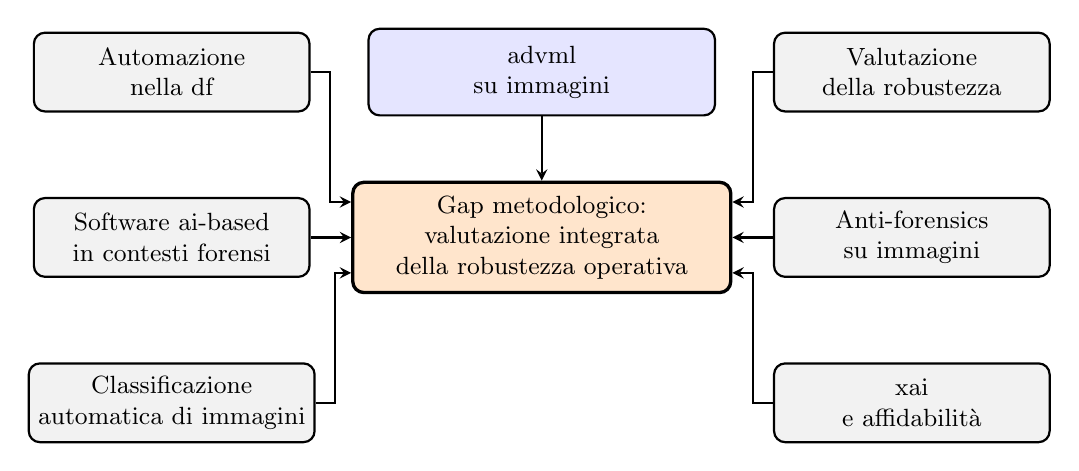
\begin{tikzpicture}[
    every node/.style={font=\small, align=center},
    field/.style={
        rectangle, rounded corners,
        draw=black, thick,
        fill=gray!10,
        minimum width=3.5cm,
        minimum height=1.0cm
    },
    central/.style={
        rectangle, rounded corners,
        draw=black, thick,
        fill=blue!10,
        minimum width=4.4cm,
        minimum height=1.1cm
    },
    gap/.style={
        rectangle, rounded corners,
        draw=black, very thick,
        fill=orange!20,
        minimum width=4.8cm,
        minimum height=1.4cm
    },
    arrow/.style={->, thick, >=stealth}
]

% Riga superiore
\node[field]   (ai_df)      at (0,   5.8) {Automazione\\nella \gls{df}};
\node[central] (advml)      at (4.7, 5.8) {\gls{advml}\\su immagini};
\node[field]   (robustness) at (9.4, 5.8) {Valutazione\\della robustezza};

% Riga centrale
\node[field] (tools)         at (0,   3.7) {Software \gls{ai}-based\\in contesti forensi};
\node[gap]   (gap)           at (4.7, 3.7) {Gap metodologico:\\valutazione integrata\\della robustezza operativa};
\node[field] (antiforensics) at (9.4, 3.7) {Anti-forensics\\su immagini};

% Riga inferiore
\node[field] (classification) at (0,   1.6) {Classificazione\\automatica di immagini};
\node[field] (xai)            at (9.4, 1.6) {\gls{xai}\\e affidabilità};

% Punti distinti di ingresso sul box gap
\coordinate (gapNW) at ([yshift=0.45cm]gap.west);
\coordinate (gapW)  at (gap.west);
\coordinate (gapSW) at ([yshift=-0.45cm]gap.west);

\coordinate (gapNE) at ([yshift=0.45cm]gap.east);
\coordinate (gapE)  at (gap.east);
\coordinate (gapSE) at ([yshift=-0.45cm]gap.east);



% Frecce da sinistra verso il gap
\draw[arrow] (ai_df.east)          -- ++(0.25,0) |- (gapNW);
\draw[arrow] (tools.east)          -- (gapW);
\draw[arrow] (classification.east) -- ++(0.25,0) |- (gapSW);

% Frecce da destra verso il gap
\draw[arrow] (robustness.west)     -- ++(-0.25,0) |- (gapNE);
\draw[arrow] (antiforensics.west)  -- (gapE);
\draw[arrow] (xai.west)            -- ++(-0.25,0) |- (gapSE);


% Freccia centrale
\draw[arrow] (advml.south) -- (gap.north);

\end{tikzpicture}

\caption{Strutturazione dei principali filoni della letteratura rispetto al gap metodologico affrontato dalla presente tesi.}
\label{fig:sota-literature-gap}
\end{figure}




Il gap specifico individuato dalla presente tesi riguarda quindi la limitata disponibilità di protocolli sperimentali integrati che combinino, nello stesso disegno valutativo, classificazione automatizzata o recupero semantico di immagini, validazione \textit{human-in-the-loop} del dataset, modelli proxy eterogenei, software AI-based selezionati per la valutazione operativa in contesto forense, perturbazioni adversariali, trasformazioni anti-forensi, metriche quantitative e analisi spiegabile del comportamento dei modelli. La rilevanza di tale integrazione deriva dal fatto che, in un contesto forense, l'affidabilità di un sistema automatico non può essere valutata soltanto come proprietà isolata del classificatore. Essa dipende anche dalla qualità e dalla rappresentatività dei dati, dalla presenza di casi borderline o fuori distribuzione, dalla natura delle manipolazioni applicate, dalla trasparenza del software impiegato e dall'effetto che eventuali errori possono produrre sul triage e sulla selezione delle evidenze.

La presente tesi si colloca precisamente in questa lacuna. Il suo contributo consiste nel condurre una valutazione sperimentale della robustezza operativa di modelli proxy e software AI-based impiegati, nel contesto della \gls{df}, per la classificazione automatizzata o il recupero semantico di immagini di potenziale interesse investigativo, considerando congiuntamente la dimensione algoritmica e quella operativo-investigativa. L'obiettivo non è soltanto misurare il degrado prestazionale in condizioni avverse, ma comprendere come tale degrado possa incidere sulla capacità del sistema di supportare l'analista nella selezione di contenuti rilevanti. In questa prospettiva, la robustezza viene trattata non come attributo astratto del modello, ma come requisito funzionale per l'uso controllato dell'\gls{ai} nei workflow di \gls{df}.

Il posizionamento della tesi è dunque duplice. Da un lato, essa si collega alla letteratura sull'\gls{advml}, sulla valutazione della robustezza e sull'\gls{xai}, assumendo che i sistemi di classificazione debbano essere valutati anche in presenza di input ostili, degradati o anomali. Dall'altro, si colloca nel dominio della \gls{df}, dove la qualità dell'automazione deve essere giudicata rispetto alla sua utilità operativa, alla verificabilità dei risultati e alla possibilità di mantenere il controllo umano sul processo di analisi. Questa impostazione consente di superare una valutazione puramente prestazionale e di affrontare il problema della robustezza come questione metodologica, tecnica e forense. Tale spazio di ricerca motiva il protocollo sperimentale \gls{fairlab}, adottato nella presente tesi e descritto nel capitolo successivo.

% ----------------- Chapter 4: Methodology ----------------------
% ─────────────────────────────────────────────────────────────────────────────
\chapter{Methodology}
\label{chap:methodology}
% ─────────────────────────────────────────────────────────────────────────────

This chapter defines the methodology adopted to evaluate the operational
robustness of \gls{ai}-based tools for automated image classification in
forensic contexts. It addresses the gap identified in
Chapter~\ref{chap:state-of-the-art} by formalizing the \gls{fairlab} framework
as a reproducible and auditable protocol that combines controlled experimental
conditions with operationally relevant forensic scenarios.

The chapter presents the overall framework and research assumptions, followed
by the procedures for dataset construction, human-in-the-loop validation,
dataset freezing and partitioning, proxy-model and black-box software
evaluation, perturbation testing, metric computation, explainability, and
traceability. Implementation-specific data structures, scripts, architectures,
parameters, software versions, and configurations are documented in
Chapter~\ref{chap:implementation}; quantitative outcomes and their
interpretation are reported in Chapter~\ref{chap:results}.

% ─────────────────────────────────────────────────────────────────────────────
\section{Overview of the FAIRLab Methodology}
\label{sec:methodology-fairlab-overview}
% ─────────────────────────────────────────────────────────────────────────────

The \gls{fairlab} protocol provides a structured framework for evaluating
automated image-classification systems under clean, \gls{ood}, adversarial,
and anti-forensic conditions. Its scope extends beyond clean classification
accuracy because automated outputs may affect evidence prioritization and the
allocation of human analytical resources. Operational robustness is therefore
examined in relation to missed relevant content, additional review workload,
and unstable behavior on inputs that differ from the expected operational
distribution.

The protocol integrates two complementary evaluation levels. The first uses
fully inspectable proxy classification models as controlled experimental
references; these models are not treated as replicas or functionally equivalent
substitutes for proprietary systems. The second evaluates selected
\gls{ai}-based software systems under black-box or near-black-box access
conditions, using only their observable inputs and outputs and making no
assumptions about inaccessible architectures, training data, calibration
procedures, or decision logic
\cite{sanna2024preliminary,sanna2025pixelperfect}.

Both levels rely on the same frozen experimental corpus. Its binary in-domain
component supports clean and perturbed evaluation, whereas a separate clean
\gls{ood} branch is evaluated outside model training and perturbation
generation, as detailed in
Section~\ref{sec:methodology-split-generation}. The clean binary samples,
clean \gls{ood} inputs, adversarial artifacts, and anti-forensic artifacts are
combined into a common evaluation bundle, enabling comparison under aligned
experimental conditions.

Quantitative metrics characterize classification performance, robustness
degradation, error direction, and \gls{ood} behavior. Explainability provides
qualitative diagnostic evidence for selected cases involving an inspectable
proxy model and is not extended to the selected black-box systems.
Traceability controls preserve the relationships among source samples, derived
artifacts, experimental conditions, observable outputs, and reported results.

The protocol specifies the methodological requirements and information that
must be preserved without prescribing particular model architectures, software
products, file formats, directory structures, databases, hashing algorithms,
or explainability techniques. These choices belong to the concrete
implementation documented in Chapter~\ref{chap:implementation}.
Figure~\ref{fig:methodology-fairlab-overview} summarizes the resulting
workflow.




\begin{figure}[H]
\centering
\resizebox{\textwidth}{!}{%
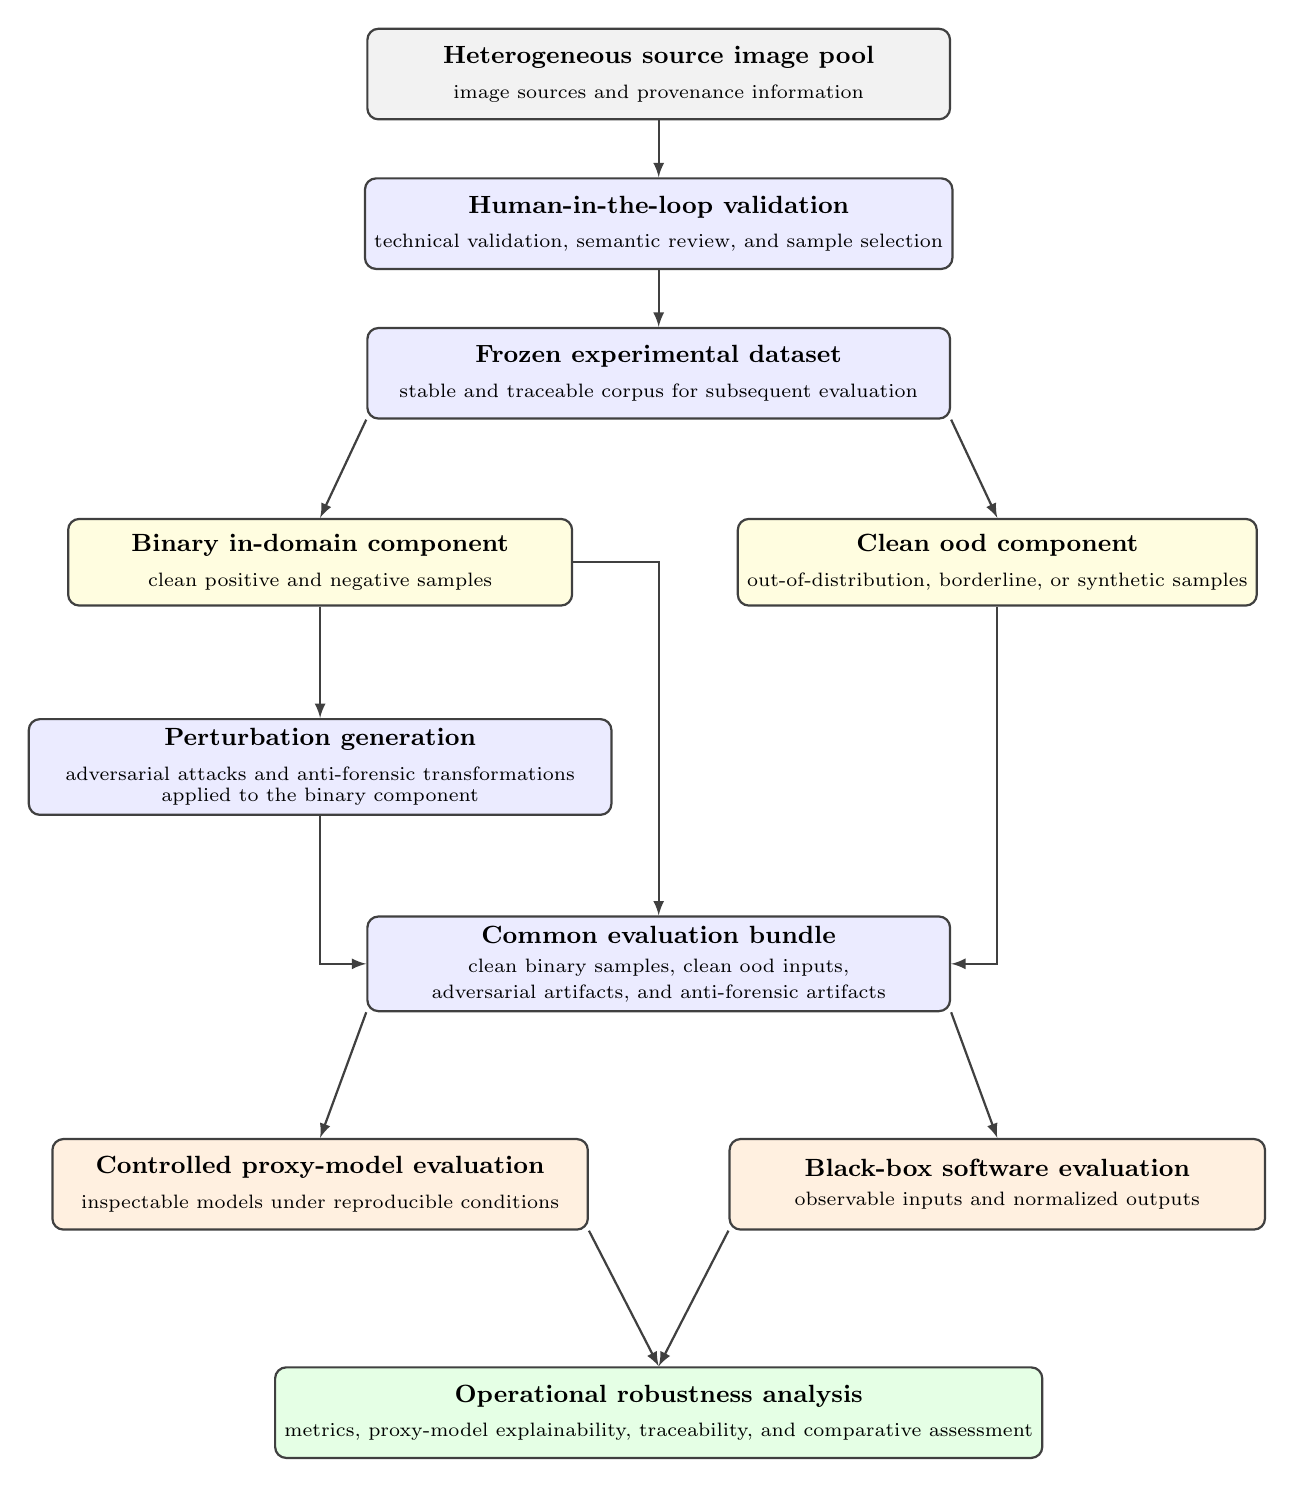
\begin{tikzpicture}[
>=latex,
font=\small,
block/.style={
rectangle,
rounded corners,
draw=black!75,
thick,
align=center,
minimum height=1.15cm,
minimum width=7.4cm,
fill=gray!10
},
process/.style={
rectangle,
rounded corners,
draw=black!75,
thick,
align=center,
minimum height=1.15cm,
minimum width=7.4cm,
fill=blue!8
},
subset/.style={
rectangle,
rounded corners,
draw=black!75,
thick,
align=center,
minimum height=1.10cm,
minimum width=6.4cm,
fill=yellow!12
},
eval/.style={
rectangle,
rounded corners,
draw=black!75,
thick,
align=center,
minimum height=1.15cm,
minimum width=6.8cm,
fill=orange!12
},
output/.style={
rectangle,
rounded corners,
draw=black!75,
thick,
align=center,
minimum height=1.15cm,
minimum width=8.0cm,
fill=green!10
},
arrow/.style={
->,
thick,
draw=black!75
}
]

% -------------------------------------------------------------------------
% Dataset construction
% -------------------------------------------------------------------------
\node[block] (sources) at (0,0)
{\shortstack{
\textbf{Heterogeneous source image pool}\\[1mm]
\scriptsize image sources and provenance information
}};

\node[process] (review) at (0,-1.9)
{\shortstack{
\textbf{Human-in-the-loop validation}\\[1mm]
\scriptsize technical validation, semantic review, and sample selection
}};

\node[process] (dataset) at (0,-3.8)
{\shortstack{
\textbf{Frozen experimental dataset}\\[1mm]
\scriptsize stable and traceable corpus for subsequent evaluation
}};

% -------------------------------------------------------------------------
% Evaluation branches
% -------------------------------------------------------------------------
\node[subset] (binary) at (-4.3,-6.2)
{\shortstack{
\textbf{Binary in-domain component}\\[1mm]
\scriptsize clean positive and negative samples
}};

\node[subset] (ood) at (4.3,-6.2)
{\shortstack{
\textbf{Clean \gls{ood} component}\\[1mm]
\scriptsize out-of-distribution, borderline, or synthetic samples
}};

% -------------------------------------------------------------------------
% Perturbation generation
% -------------------------------------------------------------------------
\node[process] (perturb) at (-4.3,-8.8)
{\shortstack{
\textbf{Perturbation generation}\\[1mm]
\scriptsize adversarial attacks and anti-forensic transformations\\
\scriptsize applied to the binary component
}};

% -------------------------------------------------------------------------
% Common evaluation bundle
% -------------------------------------------------------------------------
\node[process] (bundle) at (0,-11.3)
{\shortstack{
\textbf{Common evaluation bundle}\\[1mm]
\scriptsize clean binary samples, clean \gls{ood} inputs,\\
\scriptsize adversarial artifacts, and anti-forensic artifacts
}};

% -------------------------------------------------------------------------
% Complementary evaluation levels
% -------------------------------------------------------------------------
\node[eval] (proxy) at (-4.3,-14.1)
{\shortstack{
\textbf{Controlled proxy-model evaluation}\\[1mm]
\scriptsize inspectable models under reproducible conditions
}};

\node[eval] (tools) at (4.3,-14.1)
{\shortstack{
\textbf{Black-box software evaluation}\\[1mm]
\scriptsize observable inputs and normalized outputs
}};

% -------------------------------------------------------------------------
% Analysis layer
% -------------------------------------------------------------------------
\node[output] (analysis) at (0,-17.0)
{\shortstack{
\textbf{Operational robustness analysis}\\[1mm]
\scriptsize metrics, proxy-model explainability, traceability, and comparative assessment
}};

% -------------------------------------------------------------------------
% Arrows
% -------------------------------------------------------------------------
\draw[arrow] (sources) -- (review);
\draw[arrow] (review) -- (dataset);

\draw[arrow] (dataset.south west) -- (binary.north);
\draw[arrow] (dataset.south east) -- (ood.north);

\draw[arrow] (binary.south) -- (perturb.north);

% Direct path for the unmodified binary samples.
%\draw[arrow] (binary.west) -- ++(-1.0,0) |- (bundle.west);
\draw[arrow] (binary.east) -- ++(1.0,0) -| (bundle.north);
% Derived adversarial and anti-forensic artifacts.
\draw[arrow] (perturb.south) |- (bundle.west);

% Separate clean OOD branch.
\draw[arrow] (ood.south) |- (bundle.east);

\draw[arrow] (bundle.south west) -- (proxy.north);
\draw[arrow] (bundle.south east) -- (tools.north);

\draw[arrow] (proxy.south east) -- (analysis.north);
\draw[arrow] (tools.south west) -- (analysis.north);

\end{tikzpicture}%
}
\caption[FAIRLab experimental protocol]{FAIRLab experimental protocol. The
frozen corpus is divided into a binary in-domain component and a separate clean
\gls{ood} branch. Perturbations are applied only to the binary component, and
the resulting common bundle is evaluated through complementary proxy-model and
black-box software analyses}
\label{fig:methodology-fairlab-overview}
\end{figure}

% ─────────────────────────────────────────────────────────────────────────────
\section{Research Design and Experimental Assumptions}
\label{sec:methodology-research-design}
% ─────────────────────────────────────────────────────────────────────────────

The experimental design adopts forensic visual triage as its reference
scenario, in which automated classification supports the preliminary
identification and prioritization of potentially relevant images. The case
study defines a controlled firearm-related classification task rather than
attempting to cover the entire domain of weapon detection. This restricted
scope provides a clear target category while retaining sufficient visual
variability for robustness assessment. The adopted designations are operational
categories established for the experiment and must not be interpreted as legal
qualifications or universal semantic classes.

The binary task distinguishes between \texttt{weapon}, defined as the positive
class, and \texttt{non\_weapon}, defined as the in-domain negative class. A
separate \gls{ood} branch is reserved for distributional evaluation and is not
modeled as a third supervised class. The assignment criteria were formalized
before dataset freezing and govern human-in-the-loop validation, sample
selection, and the documentation of inclusion and exclusion decisions.
Table~\ref{tab:methodology-operational-classes} summarizes these operational
definitions.

\begin{table}[H]
\centering
\caption{Operational definitions adopted in the experimental protocol}
\label{tab:methodology-operational-classes}
\footnotesize
\renewcommand{\arraystretch}{1.05}
\begin{tabularx}{\textwidth}{@{}L{3.0cm}L{3.6cm}X@{}}
\toprule
\textbf{Designation} &
\textbf{Role in the protocol} &
\textbf{Operational assignment criterion} \\
\midrule

\texttt{weapon}
&
Positive class of the binary task
&
Images containing clearly recognizable and realistic firearm-related visual
content. Representative examples include pistols, rifles, submachine guns, and
shotguns. The target object must be sufficiently visible and reliably
attributable to the experimental category. Marginal, strongly occluded,
excessively ambiguous, synthetic, toy-like, replica-like, or airsoft-like
objects are excluded from this class. \\

\texttt{non\_weapon}
&
In-domain negative class of the binary task
&
Realistic, usable, and visually interpretable images that do not contain an
object belonging to the experimental target category. Examples may include
people, environments, vehicles, ordinary objects, and indoor or outdoor scenes.
Borderline, synthetic, or anomalous content is excluded. Images containing
knives, swords, replicas, airsoft weapons, toy weapons, videogame weapons, or
rendered weapon-like objects are also excluded because they may introduce
semantic ambiguity. \\

\gls{ood}
&
Separate branch for distributional evaluation
&
Borderline, anomalous, or non-representative images that do not constitute clean
positive or negative samples. Examples include knives, swords, replicas, toys,
airsoft weapons, videogame weapons, \gls{cgi} content, synthetic images,
generated images, tanks, missiles, explosions, and war scenes. The branch may
also include source images that are strongly degraded, unusual, or semantically
ambiguous. These inputs are retained without experimental manipulation and are
not equivalent to the adversarial or anti-forensic artifacts generated in later
stages. Such content may be contextually related to weapons or violence without
constituting a valid sample for the binary task. \\

\texttt{exclude}
&
Review-only exclusion designation
&
Images that are corrupted, unreadable, unusable, non-interpretable, or
semantically irrelevant to the experimental protocol. This designation is used
during human review to document the removal of unsuitable samples. Excluded
images do not contribute to the frozen dataset or to any subsequent evaluation
branch. \\

\bottomrule
\end{tabularx}
\end{table}

Figure~\ref{fig:methodology-class-examples} presents representative examples of
the two binary classes and the separate \gls{ood} branch. The examples are
illustrative and do not exhaust the internal variability of the corresponding
groups.

\begin{figure}[H]
\centering

\begin{minipage}[t]{0.31\textwidth}
\centering
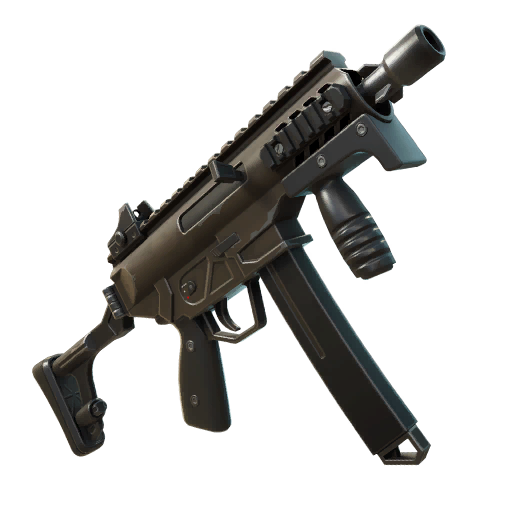
\includegraphics[
width=\textwidth,
height=4.0cm,
keepaspectratio
]{images/Arma}
\vspace{1mm}

\textbf{\texttt{weapon}}\\
\footnotesize
Recognizable firearm-related content consistent with the binary target class
\end{minipage}
\hfill
\begin{minipage}[t]{0.31\textwidth}
\centering

\includegraphics[
width=\textwidth,
height=4.0cm,
keepaspectratio
]{images/Non_Arma}
\vspace{1mm}

\textbf{\texttt{non\_weapon}}\\
\footnotesize
Realistic negative content containing no object from the target category
\end{minipage}
\hfill
\begin{minipage}[t]{0.31\textwidth}
\centering
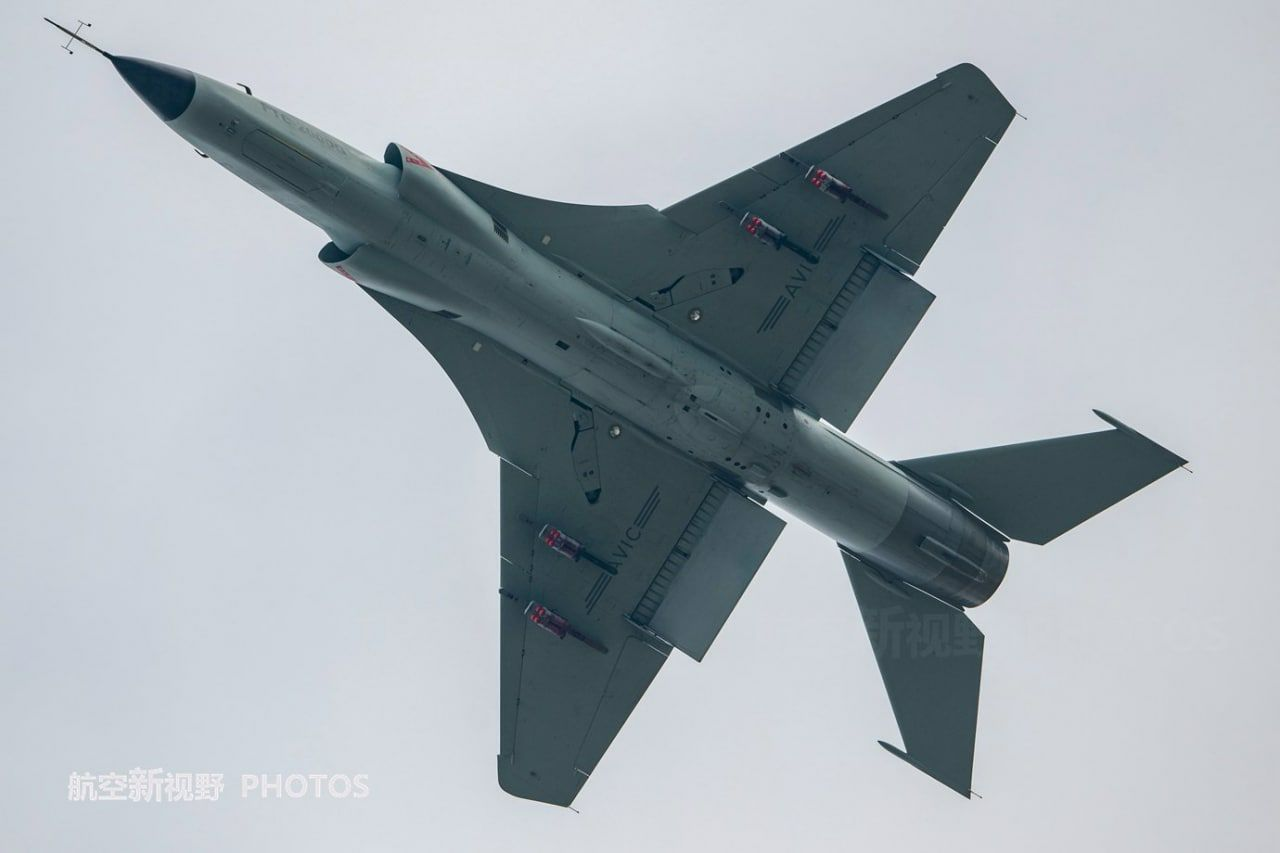
\includegraphics[
width=\textwidth,
height=4.0cm,
keepaspectratio
]{images/ood}
\vspace{1mm}

\textbf{\gls{ood}}\\
\footnotesize
Borderline or distributionally different content kept outside the binary task
\end{minipage}

\caption[Representative operational class and OOD examples]{Representative
examples of the binary operational classes and the separate \gls{ood} branch
adopted during human-in-the-loop review}
\label{fig:methodology-class-examples}
\end{figure}

The \texttt{exclude} designation is used exclusively as a quality-control
disposition during human review and does not constitute an additional
analytical branch. Likewise, the \gls{ood} branch is not a homogeneous semantic
class or a subclass of \texttt{non\_weapon}. It contains borderline,
anomalous, degraded, synthetic, or otherwise distributionally different inputs
that do not constitute clean instances of either binary class. Since
classifiers may produce high-confidence predictions outside their training
distribution \cite{hendrycks2017baseline,fort2021exploring}, these inputs must
be assessed separately from ordinary binary errors. Their exclusion from model
training and perturbation generation is formalized in
Section~\ref{sec:methodology-split-generation}.

These operational definitions provide the semantic basis for the dataset
construction, review-documentation, and freezing procedures described in
Sections~\ref{sec:methodology-dataset-construction},
\ref{sec:methodology-review-manifest}, and
\ref{sec:methodology-human-review}. They ensure that final assignments are
derived from explicit and traceable review criteria rather than inherited
directly from source labels, filenames, or directory structures.

% ─────────────────────────────────────────────────────────────────────────────
\section{Dataset Construction and Source Consolidation}
\label{sec:methodology-dataset-construction}
% ─────────────────────────────────────────────────────────────────────────────

Dataset construction separates source collection, technical validation,
semantic review, and final dataset freezing. This distinction is
methodologically necessary because the technical validity of an image file
does not establish its semantic suitability for the forensic classification
task.

The process begins with the consolidation of heterogeneous image sources into
a candidate pool. The objective is not to create a visually homogeneous
collection, but to capture part of the variability encountered in contemporary
digital investigations. Depending on the investigated domain and data
availability, the candidate pool may include public datasets, specialized
repositories, open-web content, \gls{osint}-oriented collections, and material
obtained from less structured or non-indexed online environments.

The composition and relative contribution of these sources may vary, but the
provenance of each candidate sample must remain identifiable throughout the
preparation and review process.
Table~\ref{tab:methodology-raw-sources} summarizes the methodological roles of
the source categories considered in the protocol.

\begin{table}[H]
\centering
\caption{Methodological roles of the image-source categories}
\label{tab:methodology-raw-sources}
\begin{tabularx}{\textwidth}{@{}L{4.2cm}X@{}}
\toprule
\textbf{Source category} &
\textbf{Methodological role} \\
\midrule

Public datasets
&
Provide structured and reproducible collections that can support the initial
construction of the candidate pool. Their original labels are retained as
source information and are not automatically inherited as experimentally
validated reference assignments. \\

Specialized repositories
&
Provide domain-specific images that can improve the representation of candidate
content related to the target visual category. Samples obtained from these
sources remain subject to the same validation and assignment criteria applied
to the rest of the candidate pool. \\

Open-web collections
&
Introduce greater variability in image quality, composition, context, and
acquisition conditions. They reduce dependence on curated benchmark
distributions. \\

\gls{osint}-oriented sources
&
Represent less structured content obtained from social, multimedia, or other
openly accessible investigative sources. They contribute operationally relevant
variability. \\

Non-indexed or unconventional online sources
&
Provide heterogeneous material that may differ from conventional public
datasets in content, quality, context, or distribution. Their inclusion supports
the evaluation of less standardized acquisition contexts. \\

\bottomrule
\end{tabularx}
\end{table}

After source consolidation, candidate images undergo technical validation
before any semantic assignment is made. The validation process verifies that
each file can be processed reliably and may include readability, structural
validity, dimensional suitability, duplicate detection, and stable sample
identification. The resulting records must preserve sufficient information to
associate each retained sample with its provenance, technical-validation
outcome, and integrity information.

Source location, directory structure, filename, and pre-existing annotations
may be retained as contextual or audit information, but they must not be
treated as definitive reference assignments. Final semantic membership must
instead be determined through the operational criteria defined in
Section~\ref{sec:methodology-research-design}. This separation limits the
propagation of source-specific assumptions and labeling errors into the frozen
experimental dataset.

The relative size of the original source collections must also be considered
during sample selection. A large or highly asymmetric source must not
automatically dominate the final corpus. Composition decisions should instead
reflect the experimental objectives, the required class structure, and the
need to preserve meaningful source diversity.

Following technical validation, the candidate pool is submitted to the
documented semantic-review process described in
Sections~\ref{sec:methodology-review-manifest} and
\ref{sec:methodology-human-review}. Figure~\ref{fig:methodology-dataset-source-consolidation}
summarizes the transition from heterogeneous sources to the frozen
experimental dataset.

\begin{figure}[H]
\centering
\resizebox{0.62\textwidth}{!}{%
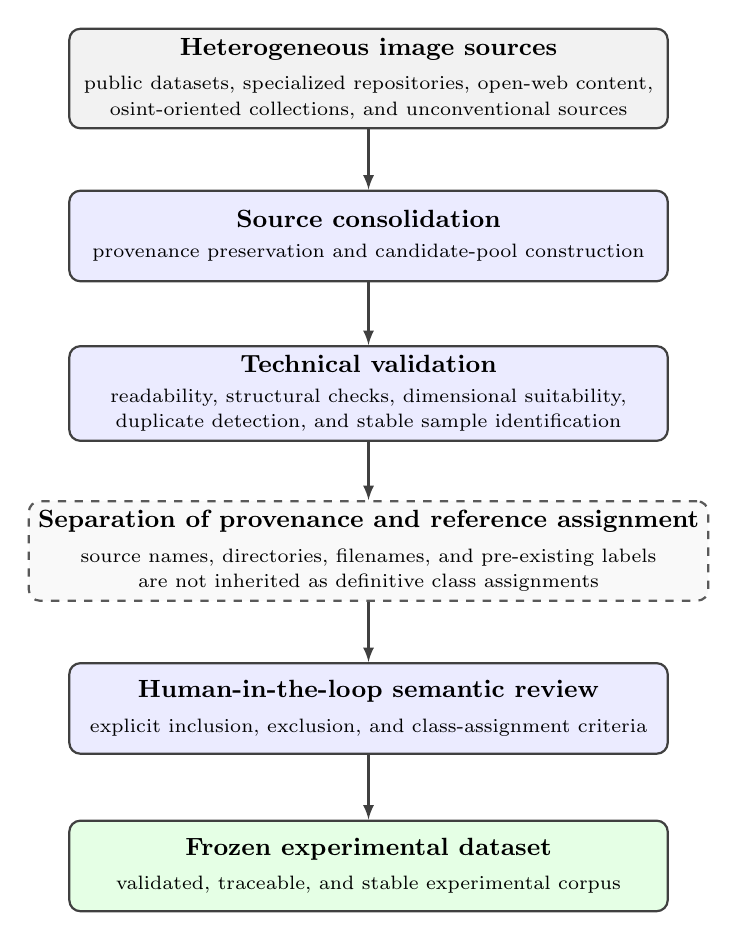
\begin{tikzpicture}[
>=latex,
font=\small,
block/.style={
rectangle,
rounded corners,
draw=black!75,
thick,
align=center,
minimum height=1.15cm,
minimum width=7.6cm,
fill=gray!10
},
process/.style={
rectangle,
rounded corners,
draw=black!75,
thick,
align=center,
minimum height=1.15cm,
minimum width=7.6cm,
fill=blue!8
},
note/.style={
rectangle,
rounded corners,
draw=black!65,
dashed,
thick,
align=center,
minimum height=1.05cm,
minimum width=7.6cm,
fill=gray!5
},
final/.style={
rectangle,
rounded corners,
draw=black!75,
thick,
align=center,
minimum height=1.15cm,
minimum width=7.6cm,
fill=green!10
},
arrow/.style={
->,
thick,
draw=black!75
}
]

\node[block] (sources) at (0,0)
{\shortstack{
\textbf{Heterogeneous image sources}\\[1mm]
\scriptsize public datasets, specialized repositories, open-web content,\\
\scriptsize \gls{osint}-oriented collections, and unconventional sources
}};

\node[process] (consolidation) at (0,-2.0)
{\shortstack{
\textbf{Source consolidation}\\[1mm]
\scriptsize provenance preservation and candidate-pool construction
}};

\node[process] (validation) at (0,-4.0)
{\shortstack{
\textbf{Technical validation}\\[1mm]
\scriptsize readability, structural checks, dimensional suitability,\\
\scriptsize duplicate detection, and stable sample identification
}};

\node[note] (separation) at (0,-6.0)
{\shortstack{
\textbf{Separation of provenance and reference assignment}\\[1mm]
\scriptsize source names, directories, filenames, and pre-existing labels\\
\scriptsize are not inherited as definitive class assignments
}};

\node[process] (review) at (0,-8.0)
{\shortstack{
\textbf{Human-in-the-loop semantic review}\\[1mm]
\scriptsize explicit inclusion, exclusion, and class-assignment criteria
}};

\node[final] (frozen) at (0,-10.0)
{\shortstack{
\textbf{Frozen experimental dataset}\\[1mm]
\scriptsize validated, traceable, and stable experimental corpus
}};

\draw[arrow] (sources) -- (consolidation);
\draw[arrow] (consolidation) -- (validation);
\draw[arrow] (validation) -- (separation);
\draw[arrow] (separation) -- (review);
\draw[arrow] (review) -- (frozen);

\end{tikzpicture}%
}
\caption[Dataset source consolidation]{Dataset source consolidation.
Heterogeneous sources are combined into a traceable candidate pool, subjected
to technical validation, and reviewed according to explicit semantic criteria.
Final class assignments are not inherited from source directories, filenames,
or pre-existing annotations}
\label{fig:methodology-dataset-source-consolidation}
\end{figure}

% ─────────────────────────────────────────────────────────────────────────────
\section{Review Documentation and Semantic Decision Records}
\label{sec:methodology-review-manifest}
% ─────────────────────────────────────────────────────────────────────────────

Following technical validation, each candidate sample is associated with a
structured review record that connects its technical preparation to the
subsequent human-in-the-loop semantic assessment. The record must preserve two
distinct categories of information: sample identity, provenance, technical
validity, and integrity information; and the semantic decision produced during
manual review, including review status, operational assignment, exclusion
disposition, explanatory notes, and any information required to document
ambiguous or \gls{ood} cases.

Regardless of its technical representation, the review record must maintain a
stable association among the candidate sample, its provenance, the documented
semantic decision, and any experimental artifact subsequently derived from it.
This association enables the decision process and the transition from the
candidate pool to the frozen experimental dataset to be reconstructed.

Labels inherited from source material or generated through automated
preprocessing may be retained as contextual information, but they must not
replace the explicit semantic judgment produced during human-in-the-loop
review. Final operational assignments are determined exclusively according to
the criteria defined in
Section~\ref{sec:methodology-research-design}.

The separation between technical-validation information and semantic decision
records preserves the distinction between file suitability and relevance to
the experimental task. The resulting documentation supports the consistent
application of the assignment criteria, preserves the rationale for inclusion,
exclusion, and class-assignment decisions, and provides the traceability
required for the review and dataset-freezing procedure described in
Section~\ref{sec:methodology-human-review}.

% ─────────────────────────────────────────────────────────────────────────────
\section{Human-in-the-Loop Review and Final Dataset Freezing}
\label{sec:methodology-human-review}
% ─────────────────────────────────────────────────────────────────────────────

The technically validated candidate pool is subjected to a documented
\textit{human-in-the-loop} review to determine the semantic suitability of each
sample and assign the corresponding operational designation. The criteria
defined in Section~\ref{sec:methodology-research-design} must be applied
consistently and independently of source directories, filenames, inherited
annotations, or automated pre-labels.

The review follows a conservative decision rule. Samples are included in the
binary task only when they can be assigned to either \texttt{weapon} or
\texttt{non\_weapon} with sufficient semantic clarity. Borderline, anomalous,
synthetic, replica-like, degraded, or otherwise distributionally different
content is retained within the separate \gls{ood} branch rather than being
forced into either binary class. Unusable or semantically irrelevant samples
are assigned to the review-only \texttt{exclude} disposition.

These assignments are operational designations defined for the experimental
protocol and must not be interpreted as definitive legal, material, or
evidentiary determinations regarding the depicted content. In particular,
assignment to the \gls{ood} branch represents a methodological decision for
cases that do not constitute clear instances of either binary class.

Each review decision must remain reconstructable through the semantic decision
records defined in Section~\ref{sec:methodology-review-manifest}. These records
preserve the association among the reviewed sample, its provenance, the
assigned disposition, any explanatory notes, and the experimental artifacts
subsequently derived from it.

After all candidate samples have been reviewed, the selected corpus is frozen.
Dataset freezing establishes a stable reference corpus whose composition
remains unchanged throughout the subsequent evaluation phases. Any correction
or modification introduced after freezing must be explicitly documented and
treated as a new version of the experimental dataset.

The frozen dataset provides the common source corpus for the controlled
proxy-model evaluation and the black-box evaluation of the selected
\gls{ai}-based software systems. Its subsequent separation into the binary
evaluation subset and the clean \gls{ood} branch is defined in
Section~\ref{sec:methodology-split-generation}.

The number of reviewers and the review workflow may vary across
implementations. When the protocol is conducted by a single reviewer, the
absence of inter-annotator agreement must be acknowledged as a limitation.
Explicit assignment criteria, structured decision records, and dataset
freezing support procedural auditability and reproducibility, but do not
eliminate the subjectivity inherent in semantic assessment. Dataset freezing
therefore acts as a methodological control that distinguishes changes in
systems, perturbations, and metrics from undocumented changes in the evaluated
corpus.











% ─────────────────────────────────────────────────────────────────────────────
\section{Data Partitioning and OOD Evaluation Strategy}
\label{sec:methodology-split-generation}
% ─────────────────────────────────────────────────────────────────────────────

After dataset freezing, the experimental corpus is divided into two distinct
branches: an in-domain binary subset and a separate \gls{ood} evaluation set.
This separation reflects the different methodological purposes of the two
components. The binary subset supports model training, clean evaluation, and
robustness testing, whereas the \gls{ood} set is used to examine system behavior
on borderline, semantically atypical, or distributionally different inputs.

The binary subset is organized into mutually exclusive experimental
partitions, hereafter referred to as folds. The number and size of these folds
depend on the available dataset, the class distribution, and the requirements
of the experimental design. The methodology therefore does not prescribe a
fixed number of folds or a specific directory organization.

Regardless of the adopted configuration, the partitioning procedure must
satisfy four requirements. First, each sample must belong to only one fold.
Second, the class distribution should remain sufficiently consistent across
folds whenever the dataset permits stratified partitioning. Third, sample
identity and provenance must remain traceable. Fourth, the allocation procedure
must be deterministic or otherwise documented in sufficient detail to allow the
partitions to be regenerated.

Within this protocol, folds are not introduced primarily as a conventional
cross-validation mechanism for hyperparameter selection or general performance
estimation. Instead, they define controlled experimental holdout units. For
each target fold, the proxy classification model is trained on the remaining
folds and evaluated on the held-out samples.

This fold-aware organization prevents overlap between the samples used for
model fitting and those used for clean and robustness evaluation. It also
preserves a consistent association between each held-out sample, the
corresponding proxy-model checkpoint, and any model-dependent adversarial
artifact generated from that sample. Model-agnostic anti-forensic
transformations remain associated with the originating sample and its assigned
fold but do not depend on a specific model checkpoint.

The specific number of folds is an implementation choice rather than a general
methodological requirement. A study may adopt a different number of partitions
provided that the resulting organization preserves separation, traceability,
and sufficient representation of the relevant classes.

The \gls{ood} samples are kept outside the binary folds. They are not used to
train the proxy classification models and are not treated as a third supervised
class. They are also excluded from the generation of adversarial and
anti-forensic variants because they address a different experimental question.

More specifically, the \gls{ood} evaluation examines how an automated system
assigns content that should not be treated as an ordinary
\texttt{weapon} or \texttt{non\_weapon} sample relative to the known
operational classes. The branch is kept clean in the methodological sense that
no experimental adversarial perturbation or anti-forensic transformation is
applied to its samples. This separation prevents distributional mismatch from
being conflated with deliberate or incidental input manipulation.

The partitioning procedure must produce structured records that associate each
sample with its evaluation branch and, when applicable, its fold. These records
should preserve sample identity, provenance, operational assignment, integrity
information, and the relationship between the original image and any derived
experimental artifact. The methodology does not impose a specific file format,
hashing algorithm, or storage technology.

Figure~\ref{fig:methodology-split-to-proxy-training} summarizes the general
partitioning strategy. The frozen dataset is separated into a binary in-domain
branch and a clean \gls{ood} branch. The binary samples are organized into
mutually exclusive folds used for fold-aware training and held-out evaluation,
whereas the \gls{ood} samples remain outside the training and perturbation
generation processes.

\begin{figure}[H]
\centering
\resizebox{0.94\textwidth}{!}{%
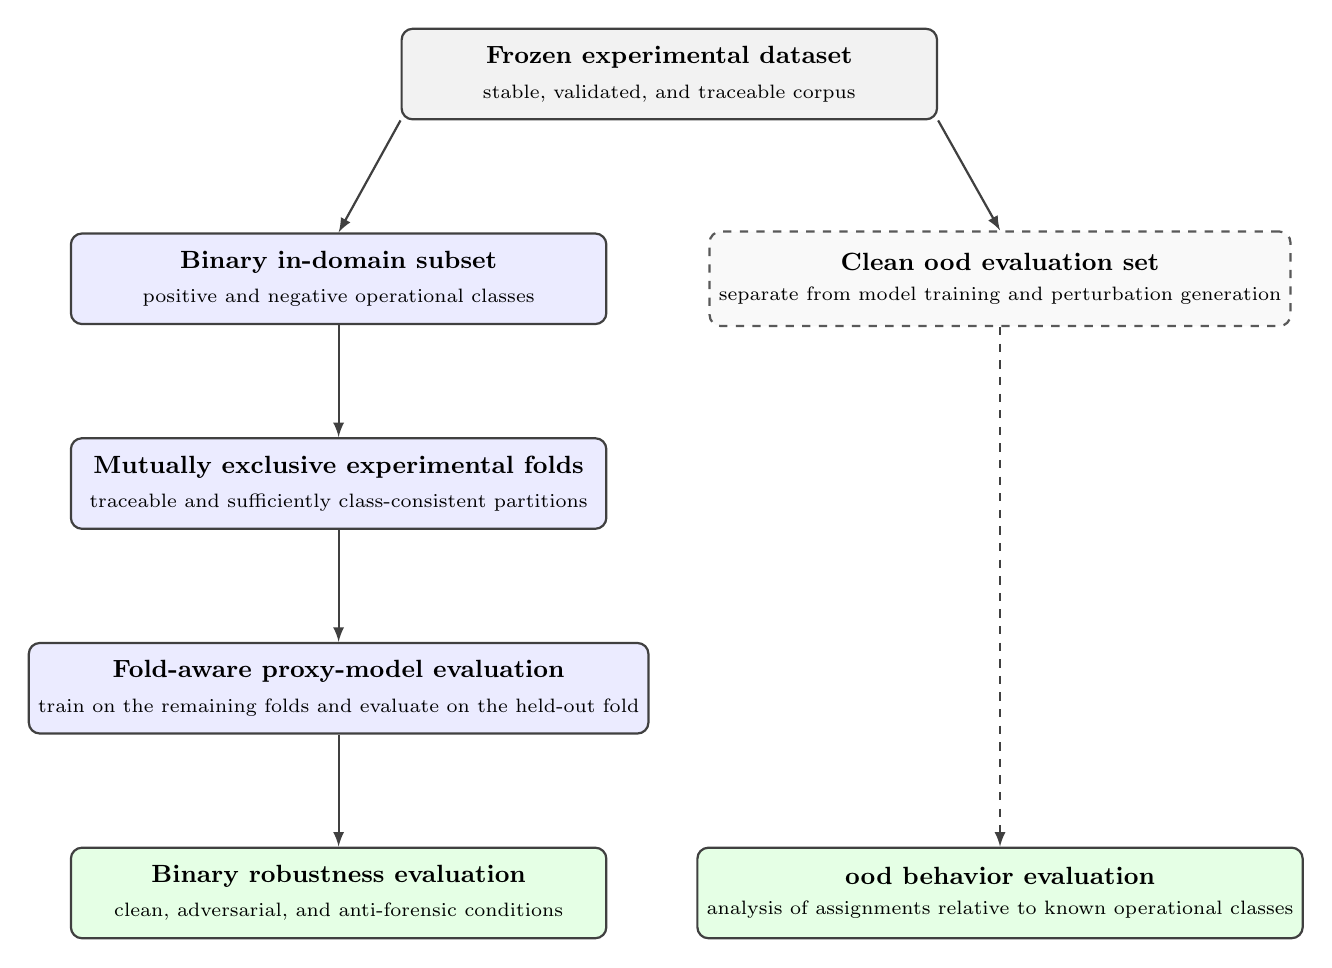
\begin{tikzpicture}[
>=latex,
font=\small,
block/.style={
rectangle,
rounded corners,
draw=black!75,
thick,
align=center,
minimum height=1.15cm,
minimum width=6.8cm,
fill=gray!10
},
process/.style={
rectangle,
rounded corners,
draw=black!75,
thick,
align=center,
minimum height=1.15cm,
minimum width=6.8cm,
fill=blue!8
},
output/.style={
rectangle,
rounded corners,
draw=black!75,
thick,
align=center,
minimum height=1.15cm,
minimum width=6.8cm,
fill=green!10
},
note/.style={
rectangle,
rounded corners,
draw=black!65,
dashed,
thick,
align=center,
minimum height=1.20cm,
minimum width=6.8cm,
fill=gray!5
},
arrow/.style={
->,
thick,
draw=black!75
},
dashedarrow/.style={
->,
thick,
dashed,
draw=black!75
}
]

\node[block] (frozen) at (0,0)
{\shortstack{
\textbf{Frozen experimental dataset}\\[1mm]
\scriptsize stable, validated, and traceable corpus
}};

\node[process] (binary) at (-4.2,-2.6)
{\shortstack{
\textbf{Binary in-domain subset}\\[1mm]
\scriptsize positive and negative operational classes
}};

\node[note] (ood) at (4.2,-2.6)
{\shortstack{
\textbf{Clean \gls{ood} evaluation set}\\[1mm]
\scriptsize separate from model training and perturbation generation
}};

\node[process] (folds) at (-4.2,-5.2)
{\shortstack{
\textbf{Mutually exclusive experimental folds}\\[1mm]
\scriptsize traceable and sufficiently class-consistent partitions
}};

\node[process] (training) at (-4.2,-7.8)
{\shortstack{
\textbf{Fold-aware proxy-model evaluation}\\[1mm]
\scriptsize train on the remaining folds and evaluate on the held-out fold
}};

\node[output] (binaryevaluation) at (-4.2,-10.4)
{\shortstack{
\textbf{Binary robustness evaluation}\\[1mm]
\scriptsize clean, adversarial, and anti-forensic conditions
}};

\node[output] (oodevaluation) at (4.2,-10.4)
{\shortstack{
\textbf{\gls{ood} behavior evaluation}\\[1mm]
\scriptsize analysis of assignments relative to known operational classes
}};

\draw[arrow] (frozen.south west) -- (binary.north);
\draw[arrow] (frozen.south east) -- (ood.north);

\draw[arrow] (binary) -- (folds);
\draw[arrow] (folds) -- (training);
\draw[arrow] (training) -- (binaryevaluation);

\draw[dashedarrow] (ood) -- (oodevaluation);

\end{tikzpicture}%
}
\caption[Data partitioning and OOD evaluation strategy]{Data partitioning and
OOD evaluation strategy. The binary subset is organized into mutually exclusive
folds for fold-aware training and held-out evaluation, while the clean
\gls{ood} branch remains outside model training and perturbation generation}
\label{fig:methodology-split-to-proxy-training}
\end{figure}


% ─────────────────────────────────────────────────────────────────────────────
\section{Proxy-Model Evaluation Framework}
\label{sec:methodology-models-classification}
% ─────────────────────────────────────────────────────────────────────────────

The controlled component of the methodology relies on a set of fully
inspectable classification models, hereafter referred to as
\textit{proxy classification models}. In this thesis, proxy models are fully
inspectable experimental reference models used to study controlled
classification behavior, robustness degradation, transferability, confidence
patterns, and error direction under reproducible conditions.

Proxy classification models are not replicas, functionally equivalent
substitutes, reverse-engineered reconstructions, or architectural reproductions
of the selected black-box software systems. Their role is to provide an
experimental environment in which model architecture, training procedure,
class mapping, checkpoints, and decision behavior can be inspected and
controlled.

The proxy-model framework supports three methodological objectives. First, it
provides a transparent reference for measuring classification performance and
robustness degradation. Second, it enables the generation of model-dependent
adversarial examples under explicitly defined access assumptions, including
white-box and score-based conditions. Third, it supports the analysis of whether
perturbations generated against one controlled model transfer to other proxy
architectures or to selected black-box software systems.

The proxy models implement the binary classification task defined in
Section~\ref{sec:methodology-research-design}. The two operational classes are
\texttt{non\_weapon} and \texttt{weapon}. Their numerical encoding is an
implementation choice and does not constitute a methodological requirement,
provided that the mapping remains explicit and consistent throughout training,
evaluation, and metric computation.

The \gls{ood} branch is excluded from proxy-model training and is not treated as
a third supervised class. It remains reserved for the separate evaluation of
system behavior on borderline, semantically atypical, or distributionally
different content, as described in
Section~\ref{sec:methodology-split-generation}. This separation prevents binary
robustness from being conflated with system behavior on samples outside the
operational distribution.

The methodology does not prescribe specific model architectures. Instead, the
controlled evaluation should include models with complementary algorithmic
characteristics. Depending on the experimental context, these may include
conventional convolutional architectures, efficiency-oriented architectures,
and models based on large-scale pretrained visual representations.

The selected models should be sufficiently documented to support reproducible
training and evaluation. Relevant information includes the architecture,
initialization strategy, preprocessing procedure, class mapping, optimization
method, training configuration, and identity of the resulting checkpoints. The
concrete architectures and configurations adopted in this thesis are reported
in Chapter~\ref{chap:implementation}.

Proxy-model training follows the fold-aware strategy introduced in
Section~\ref{sec:methodology-split-generation}. For each target fold, the
corresponding model instance is trained exclusively on the remaining folds and
evaluated on the held-out samples. This organization preserves the separation
between model fitting and experimental evaluation.

The same separation must be maintained during model-dependent perturbation
generation. An adversarial artifact associated with a held-out sample must be
generated using a model checkpoint that was not trained on that sample. This
requirement reduces the risk of information leakage and preserves the validity
of the subsequent robustness analysis.

Training conditions should remain consistent across folds for a given model
configuration. This consistency ensures that observed differences among folds
are attributable primarily to the evaluated samples rather than to unintended
changes in the optimization procedure. Any variation in architecture,
preprocessing, initialization, or training parameters must be explicitly
documented.

For model-dependent adversarial attacks, the protocol designates one controlled
model as the \textit{primary proxy target}. This model acts as the source system
against which adversarial examples are generated under the access assumptions
required by each attack. White-box attacks may use gradients, decision
boundaries, or other internal model information, whereas score-based attacks
rely on observable model scores without requiring direct access to gradients.
The choice of the primary proxy target is an implementation decision and does
not imply that the selected architecture is universally more accurate, more
representative, or more robust than the alternatives.

The use of a primary proxy target limits unnecessary multiplication of
experimental variants. Rather than optimizing every model-dependent attack
separately against every architecture, the protocol generates a coherent
adversarial test set against one documented source model. The resulting
artifacts are then evaluated on the remaining proxy models to examine
cross-model transferability.

For model-dependent adversarial artifacts, this procedure distinguishes three
evaluation conditions:

\begin{enumerate}
\item \textit{direct source-model evaluation}, in which adversarial
artifacts are assessed against the proxy-model checkpoint used to generate
them under the corresponding access assumptions;

\item \textit{cross-model transfer evaluation}, in which the same artifacts
are assessed against different proxy architectures;

\item \textit{black-box transfer evaluation}, in which the same artifacts
are submitted to the selected black-box software systems.
\end{enumerate}

Anti-forensic transformations follow a different rationale. They are applied
directly to the image according to controlled transformation rules and are not
optimized against the gradients, scores, or decision boundary of a specific
model. Their evaluation therefore concerns the stability of classification
behavior under operationally relevant image modifications rather than the
success of an optimization procedure against a designated source model.

Model-agnostic adversarial-style conditions must also be distinguished from
transfer attacks. Because they are generated without reference to a source
model, their evaluation across different proxy models and black-box software
systems measures response stability under a shared manipulated condition rather
than adversarial transferability.

The distinction among white-box, score-based, and model-agnostic conditions is
methodologically important. Model-dependent adversarial attacks evaluate
vulnerability under explicit access assumptions. Model-agnostic adversarial-
style conditions and anti-forensic transformations instead assess whether
controlled changes to image encoding, dimensions, visual quality, or appearance
alter the observable classification outcome.

Finally, the proxy-model framework must remain separate from the operational
evaluation of the selected black-box software systems. Proxy models are
inspectable and configurable components for which training conditions and model
artifacts are known. The selected software systems are evaluated under
black-box or near-black-box access conditions, without assuming access to their
internal architectures, training data, calibration procedures, or decision
logic.

This separation enables the methodology to combine experimental control with
operational relevance. Proxy models support the controlled analysis of how
documented architectures respond under reproducible conditions, while black-box
evaluation measures the observable behavior of operationally relevant software
systems when exposed to the same clean samples, clean \gls{ood} inputs,
adversarial artifacts, and anti-forensic artifacts.


% ─────────────────────────────────────────────────────────────────────────────
\section{Perturbation Selection Rationale and Operational Relevance}
\label{sec:methodology-perturbation-selection-rationale}
% ─────────────────────────────────────────────────────────────────────────────

The perturbation framework is designed to evaluate classification behavior
under controlled input modifications that differ in access assumptions,
computational cost, perceptual impact, and operational plausibility. The
selection process is therefore not based exclusively on the theoretical
strength of individual attacks. It also considers whether the resulting
experimental conditions are reproducible and relevant to realistic
\gls{df} workflows.

In forensic visual triage, automated systems may be required to process large
image collections within operational time constraints. Computational cost is
therefore methodologically relevant. A perturbation that requires extensive
optimization for each image may be useful for controlled vulnerability
analysis, but may be less representative of manipulations that can be applied
rapidly and at scale.

The methodology distinguishes among three broad categories of input
modification:

\begin{enumerate}
\item \textit{model-dependent adversarial attacks}, which are generated
against a designated source model under explicit white-box or score-based
access assumptions;

\item \textit{model-agnostic adversarial-style conditions}, which alter the
image according to predefined rules without being optimized against a
specific classifier;

\item \textit{anti-forensic transformations}, which emulate plausible
modifications of the image artifact or its visual representation.
\end{enumerate}

Model-dependent adversarial attacks provide controlled tests of classifier
vulnerability under explicit access assumptions. Depending on the selected
algorithm, they may involve a single gradient computation, an iterative
procedure, an optimization process, a decision-boundary search, or repeated
queries to observable model scores.

These attacks are included primarily to investigate sensitivity, attack
effectiveness, and transferability. They do not necessarily represent the most
probable manipulation in an ordinary forensic scenario. Their operational
relevance instead lies in demonstrating how classification behavior may change
when an actor deliberately exploits information obtained from, or interaction
with, the designated source model.

Model-agnostic adversarial-style conditions do not require access to the
internal properties or observable scores of a specific classifier. They modify
image characteristics according to predefined rules and can therefore be
generated independently of the evaluated systems. Their application across
multiple proxy architectures and black-box software systems supports comparison
under a shared manipulated condition rather than transferability analysis from
a designated source model.

Anti-forensic transformations emulate common or plausible image-processing
operations that may occur deliberately or incidentally before forensic
acquisition or analysis. Relevant transformation families include lossy
re-encoding, resampling, resizing, filtering, tonal modification, and contrast
adjustment.

Such transformations are generally inexpensive and suitable for batch
processing. They are therefore operationally relevant because they may be
applied to large collections without requiring access to the evaluated
classifier. They may also arise from ordinary image-handling processes,
including editing, forwarding, recompression, platform-mediated conversion, or
content normalization.

The perturbation set should provide complementary experimental coverage rather
than several near-duplicate variants of the same manipulation. Selection should
therefore consider the following criteria:

\begin{itemize}
\item diversity of access assumptions;
\item diversity of algorithmic mechanisms;
\item computational feasibility and scalability;
\item reproducibility across experimental runs;
\item preservation or degradation of semantic content;
\item operational plausibility;
\item suitability for cross-system comparison and, where applicable,
transferability analysis;
\item compatibility with the evaluated image formats and software systems.
\end{itemize}

Table~\ref{tab:methodology-attack-cost-operational-relevance} summarizes the
general relationship between perturbation category, computational cost, and
operational relevance.

\begin{table}[H]
\centering
\caption{Perturbation categories, computational cost, and operational relevance}
\label{tab:methodology-attack-cost-operational-relevance}
\begin{tabularx}{\textwidth}{@{}
>{\raggedright\arraybackslash}p{0.25\textwidth}
>{\raggedright\arraybackslash}p{0.18\textwidth}
X
@{}}
\toprule
\textbf{Perturbation category} &
\textbf{Typical cost} &
\textbf{Methodological and operational role} \\
\midrule

Single-step white-box attacks
&
Low to medium
&
Provide efficient baselines for evaluating sensitivity to gradient-informed
input modifications. \\

Iterative or optimization-based white-box attacks
&
Medium to high
&
Support controlled analysis of decision-boundary vulnerability and minimal or
targeted input modifications. \\

Score-based attacks
&
Medium to high
&
Evaluate vulnerability through repeated interaction with observable model
scores without requiring direct access to gradients or internal parameters. \\

Model-agnostic adversarial-style conditions
&
Low to medium
&
Enable source-model-independent testing through predefined changes to image
appearance or statistical characteristics. \\

Lossy re-encoding and resampling
&
Low
&
Represent common modifications caused by editing, forwarding, format
conversion, or platform-mediated processing. \\

Filtering and degradation
&
Low
&
Assess whether the reduction or alteration of discriminative visual details
affects classification behavior. \\

Tonal and chromatic transformations
&
Low
&
Evaluate sensitivity to changes in color, contrast, luminance, or statistical
image properties. \\

\bottomrule
\end{tabularx}
\end{table}

The cost levels reported in
Table~\ref{tab:methodology-attack-cost-operational-relevance} constitute a
qualitative methodological assessment rather than measured execution times.
Actual runtime depends on the algorithm, hardware, software libraries, image
dimensions, degree of parallelization, and implementation choices.

The qualitative distinction is based on the general algorithmic properties of
the perturbations. Direct transformations generally support efficient batch
processing. Single-step white-box attacks require limited model interaction,
whereas score-based, iterative, and optimization-based attacks may require
repeated inference, model queries, or gradient computation.

This distinction enables computational feasibility and operational plausibility
to be considered without introducing timing measurements that were not
collected systematically. The concrete attacks, transformations, parameter
values, and execution configurations adopted in this thesis are reported in
Chapter~\ref{chap:implementation}.

Adversarial and anti-forensic perturbations are generated exclusively from the
binary in-domain subset. The clean \gls{ood} set remains outside this process
because it addresses distributional mismatch rather than robustness to input
manipulation.

Each generated artifact must remain associated with its source image, the
applied perturbation family, the relevant configuration, and the evaluation
condition. For model-dependent adversarial attacks, the record must also
preserve the identity of the source-model checkpoint and the corresponding
access assumption. This association supports reproducibility and ensures that
the same artifacts can be evaluated across the proxy models and the selected
black-box software systems.

Figure~\ref{fig:methodology-perturbation-workflow} summarizes the general
perturbation workflow. The clean binary subset is processed through separate
adversarial and anti-forensic branches. The resulting artifacts are then
integrated into the common evaluation bundle, together with the unmodified
binary samples and the separate clean \gls{ood} inputs.

\begin{figure}[H]
\centering
\resizebox{0.96\textwidth}{!}{%
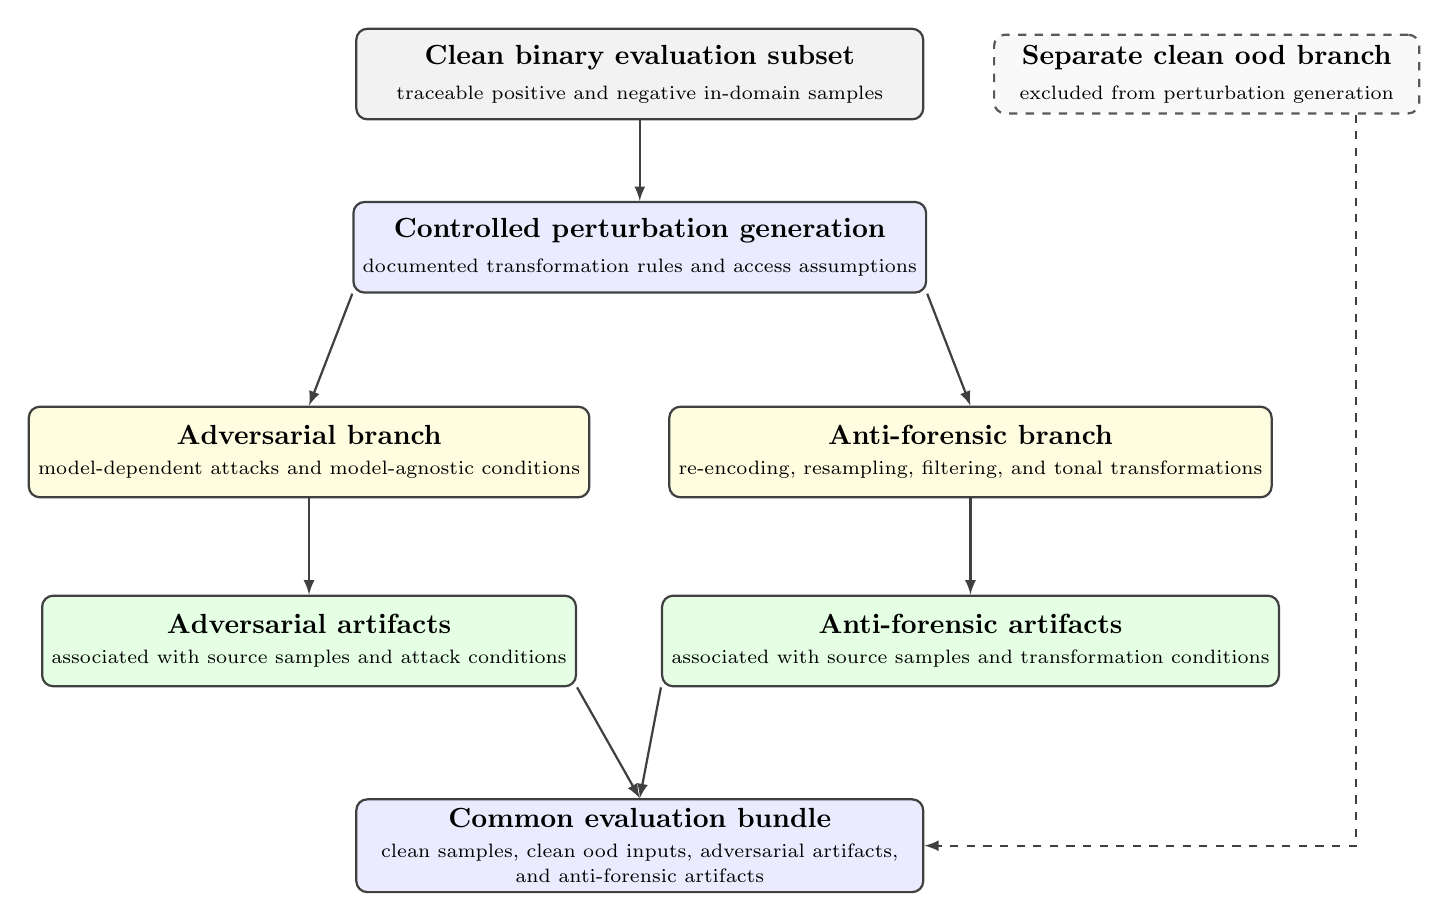
\begin{tikzpicture}[
>=latex,
font=\normalfont,
block/.style={
rectangle,
rounded corners,
draw=black!75,
thick,
align=center,
minimum height=1.15cm,
minimum width=7.2cm,
fill=gray!10
},
process/.style={
rectangle,
rounded corners,
draw=black!75,
thick,
align=center,
minimum height=1.15cm,
minimum width=7.2cm,
fill=blue!8
},
branch/.style={
rectangle,
rounded corners,
draw=black!75,
thick,
align=center,
minimum height=1.15cm,
minimum width=5.8cm,
fill=yellow!12
},
output/.style={
rectangle,
rounded corners,
draw=black!75,
thick,
align=center,
minimum height=1.15cm,
minimum width=5.8cm,
fill=green!10
},
note/.style={
rectangle,
rounded corners,
draw=black!65,
dashed,
thick,
align=center,
minimum height=1.00cm,
minimum width=5.4cm,
fill=gray!5
},
arrow/.style={
->,
thick,
draw=black!75
},
dashedarrow/.style={
->,
thick,
dashed,
draw=black!75
}
]

\node[block] (binary) at (0,0)
{\shortstack{
\textbf{Clean binary evaluation subset}\\[1mm]
\scriptsize traceable positive and negative in-domain samples
}};

\node[process] (generation) at (0,-2.2)
{\shortstack{
\textbf{Controlled perturbation generation}\\[1mm]
\scriptsize documented transformation rules and access assumptions
}};

\node[note] (ood) at (7.2,0)
{\shortstack{
\textbf{Separate clean \gls{ood} branch}\\[1mm]
\scriptsize excluded from perturbation generation
}};

\node[branch] (adversarial) at (-4.2,-4.8)
{\shortstack{
\textbf{Adversarial branch}\\[1mm]
\scriptsize model-dependent attacks and model-agnostic conditions
}};

\node[branch] (antiforensic) at (4.2,-4.8)
{\shortstack{
\textbf{Anti-forensic branch}\\[1mm]
\scriptsize re-encoding, resampling, filtering, and tonal transformations
}};

\node[output] (advartifacts) at (-4.2,-7.2)
{\shortstack{
\textbf{Adversarial artifacts}\\[1mm]
\scriptsize associated with source samples and attack conditions
}};

\node[output] (afartifacts) at (4.2,-7.2)
{\shortstack{
\textbf{Anti-forensic artifacts}\\[1mm]
\scriptsize associated with source samples and transformation conditions
}};

\node[process] (bundle) at (0,-9.8)
{\shortstack{
\textbf{Common evaluation bundle}\\[1mm]
\scriptsize clean samples, clean \gls{ood} inputs, adversarial artifacts,\\
\scriptsize and anti-forensic artifacts
}};

\draw[arrow] (binary) -- (generation);

\draw[arrow] (generation.south west) -- (adversarial.north);
\draw[arrow] (generation.south east) -- (antiforensic.north);

\draw[arrow] (adversarial) -- (advartifacts);
\draw[arrow] (antiforensic) -- (afartifacts);

\draw[arrow] (advartifacts.south east) -- (bundle.north);
\draw[arrow] (afartifacts.south west) -- (bundle.north);
\draw[dashedarrow] ([xshift=1.9cm]ood.south) |- (bundle.east);

\end{tikzpicture}%
}
\caption[Perturbation generation workflow]{Perturbation generation workflow.
Adversarial and anti-forensic artifacts are derived exclusively from the binary
subset and are integrated into the common evaluation bundle together with the
clean binary samples and the separate clean \gls{ood} inputs}
\label{fig:methodology-perturbation-workflow}
\end{figure}


% ─────────────────────────────────────────────────────────────────────────────
\section{Adversarial Evaluation Methodology}
\label{sec:methodology-adversarial-attacks}
% ─────────────────────────────────────────────────────────────────────────────

The adversarial component of the \gls{fairlab} protocol evaluates whether
controlled input modifications can alter the behavior of automated image
classifiers while preserving the relationship between each adversarial artifact
and its corresponding clean sample.

Adversarial examples are generated exclusively from the binary in-domain
subset. The clean \gls{ood} branch remains excluded because it addresses
distributional mismatch rather than robustness to deliberate input
manipulation, as established in
Section~\ref{sec:methodology-split-generation}.

The methodology distinguishes between model-dependent attacks and
model-agnostic adversarial-style conditions. Model-dependent attacks are
generated against a designated source model under explicit access assumptions.
Depending on the attack, these assumptions may include access to gradients,
decision-boundary information, internal model properties, or observable output
scores. Model-agnostic conditions instead modify the image according to
predefined rules without querying or optimizing against a specific classifier.

The selected model-dependent attacks should provide complementary coverage of
different adversarial mechanisms. Depending on the objectives of the study,
these mechanisms may include single-step gradient perturbations, sparse or
localized score-based modifications, iterative optimization procedures, and
decision-boundary-based attacks
\cite{goodfellow2015explaining,su2019onepixel,zhao2024sigmazero,moosavi2016deepfool}.

The protocol does not aim to provide an exhaustive benchmark of adversarial
robustness or a comprehensive comparison of all available attack algorithms.
Such an objective would require extensive parameter sweeps and standardized
attack suites specifically designed for adversarial machine-learning
evaluation
\cite{madry2018towards,croce2020autoattack}.

Instead, the attack set is selected to support the operational objectives of
the thesis. The selected conditions must be computationally feasible,
reproducible, sufficiently heterogeneous, and suitable for evaluating both
direct source-model vulnerability and, where applicable, transfer behavior
across different classification systems.

Model-dependent adversarial examples are generated against the primary proxy
target introduced in
Section~\ref{sec:methodology-models-classification}. For each held-out sample,
the generation process must use the fold-specific model checkpoint that was
trained without that sample. This requirement preserves the separation between
training and evaluation and prevents information leakage between the clean
input and the model used to construct its adversarial variant.

Each generated artifact must retain an explicit association with:

\begin{itemize}
\item the original clean sample;
\item the corresponding experimental fold;
\item the reference operational class;
\item the attack family or adversarial-style condition;
\item the source model, when applicable;
\item the model checkpoint or configuration used for generation, when
applicable;
\item the generation parameters;
\item the resulting output artifact;
\item the information required to verify integrity and provenance.
\end{itemize}

The methodology does not prescribe a specific manifest format, directory
structure, serialization technology, or hashing algorithm. The adopted
implementation must nevertheless preserve sufficient information to reproduce
the generation process and verify the relationship among clean inputs,
adversarial artifacts, and, where applicable, the corresponding proxy-model
configuration.

Model-agnostic adversarial-style conditions may also be included when they serve
a distinct experimental purpose. Such conditions do not constitute white-box or
score-based adversarial attacks because they are not optimized against a source
model. However, they may be evaluated within the adversarial branch when their
purpose is to examine whether controlled visual changes intended to preserve
the task-relevant semantic content alter classification behavior.

This distinction must remain explicit throughout the analysis. Model-dependent
attacks evaluate vulnerability under defined access assumptions and support
direct and transfer evaluations. Model-agnostic adversarial-style conditions
instead evaluate sensitivity to reproducible visual changes applied
independently of the evaluated models and software systems.

The output representation should minimize unintended changes unrelated to the
selected adversarial mechanism. When the chosen encoding introduces additional
compression or representation effects, those effects must be documented and
considered during interpretation.

Attack generation and robustness evaluation are treated as separate phases.
Information produced during generation, including whether an attack changed
the source-model prediction, may be retained as technical metadata. However,
such information is not treated as a final robustness result until the
generated artifacts are evaluated through the common metric and comparison
framework.

Model-dependent adversarial artifacts are subsequently evaluated under three
complementary conditions:

\begin{enumerate}
\item \textit{direct source-model evaluation}, in which each artifact is
evaluated against the fold-specific proxy-model checkpoint used for its
generation;

\item \textit{cross-model transfer evaluation}, in which the same artifact
is evaluated against different proxy architectures;

\item \textit{black-box transfer evaluation}, in which the same artifact is
submitted to the selected black-box software systems to examine observable
transfer behavior.
\end{enumerate}

Model-agnostic adversarial-style artifacts are evaluated across the proxy models
and selected black-box software systems under the same manipulated condition.
Because these artifacts are not generated against a designated source model,
differences in system behavior are interpreted as response variation under a
shared condition rather than as adversarial transferability.

The specific attack algorithms, model configurations, parameter values, output
formats, and traceability artifacts adopted in this thesis are reported in
Chapter~\ref{chap:implementation}.


% ─────────────────────────────────────────────────────────────────────────────
\section{Anti-Forensic Evaluation Methodology}
\label{sec:methodology-anti-forensic-transformations}
% ─────────────────────────────────────────────────────────────────────────────

The anti-forensic component of the \gls{fairlab} protocol evaluates the
stability of automated image classification under controlled and operationally
plausible modifications of the image artifact.

Unlike the model-dependent attacks described in
Section~\ref{sec:methodology-adversarial-attacks}, anti-forensic
transformations are not optimized against the gradients, loss function,
observable output scores, or decision boundary of a specific classifier. They
are applied according to predefined image-processing rules and can therefore be
evaluated consistently across different proxy models and selected black-box
software systems.

The term \textit{anti-forensic} is used in an experimental and operational
sense. It does not necessarily imply malicious intent or deliberate evidence
concealment. Instead, it identifies transformations that may alter, degrade, or
destabilize automated analysis by modifying the visual, statistical, or
encoding-related characteristics of an image.

Such transformations may be introduced deliberately, but they may also arise
from ordinary image-handling processes. Examples include repeated saving,
format conversion, platform-mediated recompression, resizing, forwarding,
filtering, enhancement, or normalization. Their effects are therefore relevant
to both deliberate anti-forensic scenarios and incidental preprocessing
conditions.

The methodology considers transformation families that affect complementary
properties of the image artifact. These include lossy re-encoding, spatial
resampling, blurring, tonal-distribution modification, and contrast adjustment.
The specific algorithms and parameter values used to instantiate these
families are implementation choices documented in
Chapter~\ref{chap:implementation}.

Table~\ref{tab:methodology-anti-forensic-transformations} summarizes the
methodological roles of the principal transformation families.

\begin{table}[H]
\centering
\caption{Methodological roles of the anti-forensic transformation families}
\label{tab:methodology-anti-forensic-transformations}
\begin{tabularx}{\textwidth}{@{}
>{\raggedright\arraybackslash}p{0.28\textwidth}
X
@{}}
\toprule
\textbf{Transformation family} &
\textbf{Methodological role} \\
\midrule

Lossy re-encoding
&
Evaluates classification stability when the image representation is altered by
compression artifacts or repeated encoding. \\

Spatial resampling and resizing
&
Examines sensitivity to resolution changes, interpolation, and repeated
downsampling or restoration operations. \\

Blurring and local-detail degradation
&
Assesses the dependence of automated classification on edges, textures, and
other high-frequency visual information. \\

Tonal-distribution modification
&
Evaluates sensitivity to changes in the statistical distribution of image
intensities. \\

Contrast adjustment
&
Examines whether normalization or enhancement of the intensity range alters the
classification outcome. \\

\bottomrule
\end{tabularx}
\end{table}

The transformations are applied exclusively to the binary in-domain subset.
The clean \gls{ood} branch remains separate because it addresses
distributional mismatch rather than robustness to image manipulation.

Each transformation must be applied through a consistent and documented
procedure across the selected experimental samples. The transformation rules
and their parameter values must remain fixed within a given experimental
condition unless a parameter-sensitivity analysis is explicitly included in the
research design. This consistency supports comparison across models, folds,
classes, and software systems.

The selected settings should introduce controlled and interpretable
modifications while preserving sufficient task-relevant semantic content for
meaningful evaluation. The objective is not to make the images unrecognizable,
but to examine whether operationally plausible changes can alter the behavior
of automated classification systems.

The methodology does not require an exhaustive catalog of anti-forensic
techniques. Instead, the selected transformation set should provide
complementary coverage of encoding, spatial, filtering, tonal, and contrast
effects. The selection should also consider reproducibility, computational
feasibility and scalability, compatibility with the evaluated systems, and the
possibility of applying the transformations consistently to the complete
experimental subset.

For every generated artifact, the implementation must preserve the association
with the corresponding clean sample, reference operational class, experimental
fold, and transformation condition. It must also record the applied
configuration and the information required to verify artifact identity,
integrity, and provenance.

The methodology does not prescribe a specific directory structure, manifest
format, database technology, or hashing algorithm. However, the adopted
implementation must make it possible to reconstruct the relationship among the
clean image, the applied transformation, and the resulting artifact.

Anti-forensic artifact generation and robustness evaluation are treated as
separate phases. Successful generation and completion of technical integrity
checks demonstrate that the intended experimental artifacts were produced
correctly, but do not establish robustness degradation. The impact of the
transformations must instead be determined through subsequent evaluation using
the common metrics and comparison framework.

The generated artifacts are evaluated on both the proxy classification models
and the selected black-box software systems. This common evaluation supports a
structured comparison between controlled model behavior and the observable
operational behavior of the selected software systems under the same
anti-forensic conditions.


% ─────────────────────────────────────────────────────────────────────────────
\section{Forensic Evaluation Bundle and Blind-Input Design}
\label{sec:methodology-forensic-evaluation-bundle}
% ─────────────────────────────────────────────────────────────────────────────

The operational evaluation of selected black-box software systems requires the
experimental inputs to be transferred without exposing descriptors that could
reveal their reference class, provenance, perturbation condition, or expected
operational assignment. For this purpose, the \gls{fairlab} protocol introduces
a \textit{forensic evaluation bundle}: a controlled and traceable collection of
clean binary samples, clean \gls{ood} inputs, adversarial artifacts, and
anti-forensic artifacts prepared for black-box evaluation.

The bundle does not alter the reference operational assignments, the clean
samples, or the generated artifacts. Its methodological function is to separate
the inputs submitted to the evaluated software systems from the information
required for subsequent normalization, verification, and analysis.

This separation supports two complementary views of the same experimental
corpus:

\begin{enumerate}
\item a \textit{blind input view}, containing only the files submitted to
the evaluated software systems;

\item a \textit{control and audit view}, preserving the associations among
each submitted file, its source sample, reference operational assignment,
experimental family, perturbation condition, provenance, and integrity
information.
\end{enumerate}

The blind input view must avoid experimental descriptors in filenames,
directory names, and paths. In particular, the submitted files must not expose
the reference operational class, fold assignment, attack family,
transformation type, proxy model, or any other descriptor generated by the
experimental pipeline.

This requirement reduces the risk that either the software system or the
analyst may infer the experimental role of a sample from its organization
rather than from the submitted image itself. Neutral identifiers should
therefore be assigned to the files, while the mapping to the corresponding
reference assignments and experimental conditions must remain available only
within the separate control records. The blind-input design does not conceal
the visual content or the effects of the applied perturbation, because these
constitute the actual inputs under evaluation.

The control and audit view must preserve sufficient information to reconstruct
the identity and experimental role of every submitted file. Relevant
information includes:

\begin{itemize}
\item a neutral bundle identifier;
\item the corresponding source-image identifier;
\item the reference operational assignment;
\item the experimental family;
\item the attack or transformation condition, when applicable;
\item the fold or evaluation partition;
\item provenance information;
\item integrity information;
\item the path or identifier used in the blind input view.
\end{itemize}

The methodology does not prescribe a specific directory structure, manifest
format, database technology, or naming convention. The adopted implementation
must nevertheless ensure that the blind software input remains operationally
separated from the experimental metadata and control records.

Table~\ref{tab:methodology-forensic-bundle-layout} summarizes the methodological
components of the forensic evaluation bundle.

\begin{table}[H]
\centering
\caption{Methodological components of the forensic evaluation bundle}
\label{tab:methodology-forensic-bundle-layout}
\begin{tabularx}{\textwidth}{@{}L{4.0cm}X@{}}
\toprule
\textbf{Component} &
\textbf{Methodological function} \\
\midrule

Blind input view
&
Contains only neutrally identified files submitted to the evaluated software
systems. It must not expose reference classes, perturbation families, folds,
model names, or other experimental descriptors through filenames, paths, or
directory organization. \\

Control metadata
&
Preserves the mapping between each blind identifier and the corresponding
source sample, reference operational assignment, experimental condition,
provenance, and integrity information. \\

Structured audit view
&
Provides an internal organization of the experimental inputs and derived
artifacts for technical verification and inspection. It is not submitted to the
evaluated software systems. \\

Integrity and consistency records
&
Document file identity, uniqueness, completeness, and correspondence with the
source records produced during the preceding experimental phases. \\

Embedded-information audit
&
Examines whether image files contain metadata or other machine-readable fields
that could reveal provenance, processing history, or experimental information
not concealed through neutral filenames and paths. \\

\bottomrule
\end{tabularx}
\end{table}

Only the blind input view is submitted to the evaluated software systems.
Control metadata and structured audit records remain external to the import
process and are used after the software outputs have been exported.

This separation also prevents the evaluated systems from receiving reference
assignment information through the organization of the experimental corpus.
The resulting outputs can therefore be aligned with the control records only
during the normalization and analysis phases.

The blindness of the bundle primarily concerns information channels directly
controlled by the experimental pipeline, including filenames, paths, directory
structure, and accompanying metadata files. However, image files may also
contain embedded information related to acquisition devices, processing
software, provenance, or content descriptors
\cite{xiang2021forensicmetadata,lee2023forensicmethodology,zheng2023exif}.

For this reason, the bundle-construction process should include an audit of
embedded metadata and other machine-readable information that could reveal
provenance or experimental information. The audit should identify potentially
informative fields without modifying the evaluated files unless metadata
removal or normalization is explicitly included in the research design.

The presence of embedded metadata must be treated as a documented limitation of
the blind-input design rather than as a robustness result. Any relationship
between such metadata and the observable outputs of the evaluated systems must
be investigated separately as a potential sensitivity condition.

The bundle must include all experimental families required by the protocol and
must preserve their expected composition. Completeness and uniqueness checks
should verify that no required input or derived artifact is missing, duplicated,
or incorrectly associated with the corresponding control record.

These controls establish the technical validity of the evaluation corpus but do
not constitute evidence of classification performance or operational
robustness. Quantitative bundle composition and integrity outcomes are
documented in Chapter~\ref{chap:implementation}, whereas the observed software
outputs are analyzed in Chapter~\ref{chap:results}.

The selected software systems are evaluated under black-box or near-black-box
access conditions. The methodology does not assume access to their internal
architectures, training data, decision thresholds, output-score calibration, or
proprietary decision logic. Evaluation is based exclusively on the files
submitted to the systems and on the outputs that can be observed or exported.

After processing, the software outputs are normalized against the control
metadata of the bundle. This normalization reconstructs the relationship
between each blind identifier and its reference operational assignment and
experimental condition, enabling consistent metric computation across
heterogeneous software systems.

The forensic evaluation bundle therefore represents the controlled interface
between the reproducible experimental pipeline and the selected black-box
software environments. It preserves descriptor-level blindness during import,
traceability during normalization, and comparability during evaluation. The
resulting assessment is specific to the evaluated versions, configurations,
input corpus, and output mappings and must not be interpreted as a general
validation or certification of the selected software systems
\cite{sanna2024preliminary,sanna2025pixelperfect}.


% ─────────────────────────────────────────────────────────────────────────────
\section{Black-Box Software Evaluation Protocol}
\label{sec:methodology-forensic-tools}
% ─────────────────────────────────────────────────────────────────────────────

The operational component of the \gls{fairlab} methodology evaluates software
systems that provide automated or \gls{ai}-assisted functionality for image
classification, semantic retrieval, multimedia triage, or forensic review.

Unlike the proxy classification models described in
Section~\ref{sec:methodology-models-classification}, these systems are evaluated
under black-box or near-black-box access conditions. The evaluation does not
assume access to their internal architectures, training data, model weights,
decision thresholds, calibration procedures, or proprietary inference logic.
It is based exclusively on the inputs submitted to the software systems and on
the outputs that can be observed or exported.

The purpose of this phase is not to validate or certify the selected software
systems or to rank heterogeneous systems in absolute terms. Instead, the
protocol examines their observable operational behavior under controlled and
reproducible conditions. The same clean binary samples, clean \gls{ood} inputs,
adversarial artifacts, and anti-forensic artifacts used in the controlled
experimental pipeline are submitted to the selected software systems.

This design creates two complementary evaluation levels. Proxy models provide
an inspectable environment for studying controlled model behavior, adversarial
artifact generation, and transferability. Black-box software evaluation instead
measures the observable behavior of operationally relevant systems whose
internal decision processes are not fully accessible.

The evaluation begins with the blind input view of the forensic evaluation
bundle described in
Section~\ref{sec:methodology-forensic-evaluation-bundle}. Only neutrally
identified image files are imported or indexed. Experimental metadata,
structured audit records, reference operational assignments, fold allocations,
perturbation names, and other experimental descriptors remain outside the
software environment.

This separation reduces the risk of descriptor-induced and analyst-induced
bias. Neither the software system nor the analyst should be able to infer the
expected operational assignment or evaluation condition from filenames,
directories, or associated control records during import and processing. The
visual content of the submitted images and the effects of any applied
perturbations remain visible because they constitute the actual inputs under
evaluation.

The selected software systems may expose heterogeneous types of output.
Depending on the system and its operational paradigm, observable outputs may
include:

\begin{itemize}
\item assigned categories or labels;
\item semantic tags or bookmarks;
\item retrieval results generated from textual or visual queries;
\item system-specific output scores or ranking values;
\item detected-item lists;
\item exported reports or structured records;
\item missing, ambiguous, unsupported, or non-interpretable output states.
\end{itemize}

These outputs do not necessarily correspond directly to the operational classes
defined by the experimental protocol. A software system may use proprietary
categories, broader semantic labels, hierarchical bookmarks, retrieval ranks,
or system-specific output scores. Consequently, an explicit normalization
procedure is required before quantitative comparison.

The normalization process consists of three main stages:

\begin{enumerate}
\item matching each exported output to the corresponding blind bundle
input;

\item interpreting the observable software output according to a documented
software-specific mapping rule;

\item recoding the result into a common set of operational prediction states
suitable for metric computation.
\end{enumerate}

Input matching may rely on neutral bundle identifiers, filenames,
cryptographic hashes, or other stable identifiers exposed by the software
system. The matching procedure must preserve the connection between each
exported result and the corresponding control record without exposing the
reference operational assignment during software processing.

The software-specific mapping rule must be established and documented before
the final quantitative analysis. It should identify which observable
categories, tags, bookmarks, or retrieval outcomes constitute evidence that
the software system flagged the target class.

The absence of a target-related output must not be interpreted as an absolute
semantic statement about the image. It indicates only that the software system
did not produce the relevant observable output under the tested configuration.

Similarly, outputs that cannot be mapped reliably must not be forced into a
positive or negative prediction. The protocol therefore preserves an explicit
\texttt{unknown} state for missing, ambiguous, unsupported, unmapped, or
non-interpretable outputs.

This distinction is essential because unknown outputs and explicit negative
predictions represent different observable states. They must remain separate in
the normalized records. When a documented risk-oriented analysis treats an
unknown output on a \texttt{weapon} sample as a missed detection, the unknown
state must nevertheless remain separately reportable. Conversely, treating
every semantically related output as a positive detection may inflate
false-positive counts. The normalization criteria must therefore remain
conservative, explicit, and traceable.

Table~\ref{tab:methodology-tool-normalization-summary} summarizes the general
normalization principles applied to heterogeneous black-box outputs.

\begin{table}[H]
\centering
\caption{General normalization principles for black-box software outputs}
\label{tab:methodology-tool-normalization-summary}
\footnotesize
\renewcommand{\arraystretch}{1.15}
\begin{tabularx}{\textwidth}{@{}L{4.0cm}X@{}}
\toprule
\textbf{Observable output condition} &
\textbf{Operational normalization principle} \\
\midrule

Target-related category, tag, or bookmark
&
Recoded as a positive detection only when the exported output is explicitly
associated with the target category according to the documented mapping rule. \\

Semantic retrieval result
&
Recoded according to a predefined retrieval rule that specifies the accepted
queries, configurations, and aggregation procedure. \\

No target-related output
&
Recorded as no target detection under the tested configuration. This state does
not constitute independent semantic evidence that the target object is absent. \\

Ambiguous or broader semantic output
&
Preserved as \texttt{unknown} unless the mapping rule establishes a sufficiently
precise relationship with the target class. \\

Missing, unsupported, unmapped, or non-interpretable output
&
Preserved as \texttt{unknown} in the normalized records. For
\texttt{weapon} samples, this state may contribute to an operational
missed-detection count under a documented risk-oriented rule while remaining
separately reportable. \\

\bottomrule
\end{tabularx}
\end{table}

Software configuration is an implementation-specific aspect of the protocol.
For each evaluated system, the category, query, module, plugin, or processing
function that most closely corresponds to the experimental target must be
selected and documented. When multiple reasonable configurations are available,
a sensitivity analysis may be performed to determine how configuration changes
affect detection coverage and false-positive behavior.

The methodology does not prescribe specific software systems, versions,
graphical interfaces, category names, semantic prompts, or threshold values.
Such elements may change across software releases and operational environments.
The concrete systems and configurations used in this thesis are documented in
Chapter~\ref{chap:implementation}.

For every evaluated system, the protocol follows the same general workflow:

\begin{enumerate}
\item import or index only the blind evaluation inputs;

\item enable the relevant automated analysis or retrieval functionality;

\item process the complete blind input view under a documented
configuration;

\item export all observable outputs required for subsequent matching and
interpretation;

\item align the exported records with the experimental control metadata;

\item normalize the software-specific outputs into common operational
prediction states;

\item compute comparable metrics while preserving unknown outcomes.
\end{enumerate}

Raw exports, normalization records, and aggregated metrics must remain separate.
The raw export preserves the software output as originally produced. The
normalization record documents the matching and recoding decisions. The metric
files contain only the quantitative results derived after normalization.

This separation preserves a traceability chain among the submitted bundle
input, the observable software output, the applied mapping rule, and the
resulting prediction state. It also enables normalization errors or ambiguous
mappings to be reviewed without repeating the entire software execution.

The output categories produced by the selected black-box software systems must
not be interpreted as local explanations of their internal decision processes.
A tag, bookmark, classification, or retrieval result is treated only as an
observable black-box output. The methodology does not infer which internal
features, models, or decision mechanisms caused that output.

The resulting evaluation is therefore anchored to externally verifiable
behavior. It measures whether the selected software systems produce
operationally relevant outputs for the submitted inputs without attributing
internal properties that cannot be independently verified
\cite{sanna2024preliminary,sanna2025pixelperfect}.

Figure~\ref{fig:methodology-forensic-tool-workflow} summarizes the general
black-box evaluation workflow. The software systems receive only the blind
bundle input. Reference operational assignments and experimental metadata
remain separate until the output-matching and normalization stages.

\begin{figure}[H]
\centering
\resizebox{0.96\textwidth}{!}{%
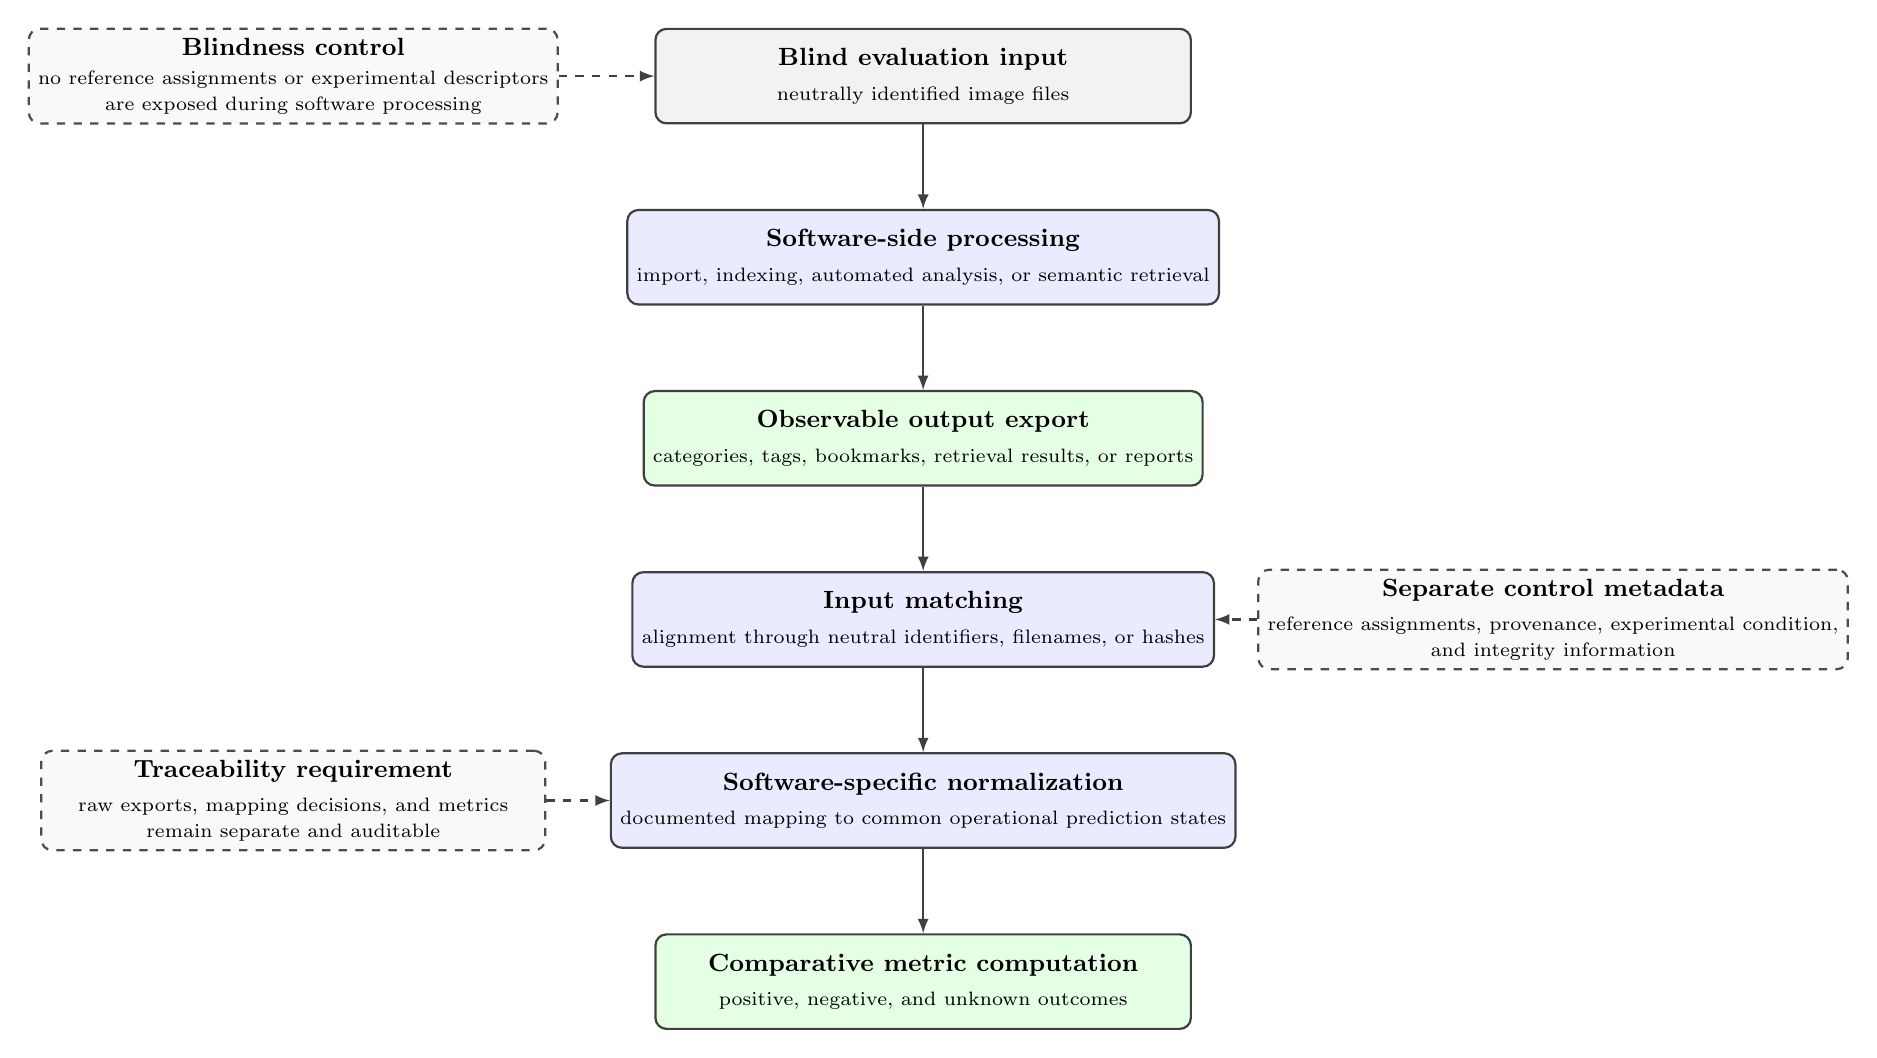
\begin{tikzpicture}[
>=latex,
font=\small,
block/.style={
rectangle,
rounded corners,
draw=black!75,
thick,
align=center,
minimum height=1.20cm,
minimum width=6.8cm,
fill=gray!10
},
process/.style={
rectangle,
rounded corners,
draw=black!75,
thick,
align=center,
minimum height=1.20cm,
minimum width=6.8cm,
fill=blue!8
},
output/.style={
rectangle,
rounded corners,
draw=black!75,
thick,
align=center,
minimum height=1.20cm,
minimum width=6.8cm,
fill=green!10
},
note/.style={
rectangle,
rounded corners,
draw=black!70,
dashed,
thick,
align=center,
minimum height=1.15cm,
minimum width=6.4cm,
fill=gray!5
},
arrow/.style={
->,
thick,
draw=black!75
},
dashedarrow/.style={
->,
thick,
dashed,
draw=black!75
}
]

\node[block] (blind) at (0,0)
{\shortstack{
\textbf{Blind evaluation input}\\[1mm]
\scriptsize neutrally identified image files
}};

\node[process] (processing) at (0,-2.3)
{\shortstack{
\textbf{Software-side processing}\\[1mm]
\scriptsize import, indexing, automated analysis, or semantic retrieval
}};

\node[output] (export) at (0,-4.6)
{\shortstack{
\textbf{Observable output export}\\[1mm]
\scriptsize categories, tags, bookmarks, retrieval results, or reports
}};

\node[process] (matching) at (0,-6.9)
{\shortstack{
\textbf{Input matching}\\[1mm]
\scriptsize alignment through neutral identifiers, filenames, or hashes
}};

\node[process] (normalization) at (0,-9.2)
{\shortstack{
\textbf{Software-specific normalization}\\[1mm]
\scriptsize documented mapping to common operational prediction states
}};

\node[output] (metrics) at (0,-11.5)
{\shortstack{
\textbf{Comparative metric computation}\\[1mm]
\scriptsize positive, negative, and unknown outcomes
}};

\node[note] (blindness) at (-8.0,0)
{\shortstack{
\textbf{Blindness control}\\[1mm]
\scriptsize no reference assignments or experimental descriptors\\
\scriptsize are exposed during software processing
}};

\node[note] (metadata) at (8.0,-6.9)
{\shortstack{
\textbf{Separate control metadata}\\[1mm]
\scriptsize reference assignments, provenance, experimental condition,\\
\scriptsize and integrity information
}};

\node[note] (traceability) at (-8.0,-9.2)
{\shortstack{
\textbf{Traceability requirement}\\[1mm]
\scriptsize raw exports, mapping decisions, and metrics\\
\scriptsize remain separate and auditable
}};

\draw[arrow] (blind) -- (processing);
\draw[arrow] (processing) -- (export);
\draw[arrow] (export) -- (matching);
\draw[arrow] (matching) -- (normalization);
\draw[arrow] (normalization) -- (metrics);

\draw[dashedarrow] (blindness.east) -- (blind.west);
\draw[dashedarrow] (metadata.west) -- (matching.east);
\draw[dashedarrow] (traceability.east) -- (normalization.west);

\end{tikzpicture}%
}
\caption[Black-box software evaluation workflow]{Black-box software evaluation
workflow. Neutrally identified inputs are processed without access to reference
operational assignments or experimental descriptors. Observable outputs are
subsequently matched to the control metadata, normalized through documented
software-specific rules, and converted into common operational prediction
states}
\label{fig:methodology-forensic-tool-workflow}
\end{figure}


% ─────────────────────────────────────────────────────────────────────────────
\section{Evaluation Metrics}
\label{sec:methodology-evaluation-metrics}
% ─────────────────────────────────────────────────────────────────────────────

The \gls{fairlab} metric framework evaluates three complementary dimensions of
operational robustness: binary classification performance under clean
conditions, robustness under adversarial and anti-forensic conditions, and
system behavior on \gls{ood} inputs. The framework also supports the evaluation
of selected black-box software systems after their heterogeneous outputs have
been normalized into common operational prediction states.

The objective is not limited to aggregate classification accuracy. In forensic
visual triage, different error types may have different operational
consequences. A false negative on a \texttt{weapon} sample may prevent
target-category content from being prioritized for detailed review. A false
positive may instead increase the volume of non-target material submitted to
the analyst.

The evaluation framework therefore combines conventional classification
metrics with condition-specific robustness indicators and operationally
oriented error measures. Binary metrics are computed separately for clean,
adversarial, and anti-forensic conditions. The \gls{ood} branch is evaluated
through separate behavioral indicators and is not integrated into the binary
confusion matrix.

The protocol does not adopt \gls{auroc} as a central metric. Although
score-based measures are widely used in supervised \gls{ml}, their consistent
application requires comparable continuous outputs across the evaluated
systems. The proxy models expose continuous prediction outputs, whereas the
selected black-box software systems may provide only categorical labels,
semantic tags, bookmarks, retrieval results, or system-specific scores whose
meaning and calibration cannot be independently verified.

The metric framework consequently prioritizes measures that can be derived
consistently from both inspectable models and normalized black-box outputs. This
choice does not imply a theoretical limitation of \gls{auroc} or other
score-based metrics. It reflects the operational requirement to compare
heterogeneous systems without assuming that their output scores have equivalent
meaning or calibration.

For the binary classification task, the principal metrics are accuracy,
balanced accuracy, precision, recall, F1-score, and the confusion matrix.
Class-specific interpretation is required because aggregate performance may
conceal asymmetric error behavior between the \texttt{weapon} and
\texttt{non\_weapon} classes.

Let \(TP\), \(TN\), \(FP\), and \(FN\) denote the numbers of true positives,
true negatives, false positives, and false negatives, respectively. Accuracy is
defined as:

\begin{equation}
\mathrm{Accuracy}
=
\frac{TP + TN}{TP + TN + FP + FN}
\end{equation}

Recall for the positive \texttt{weapon} class is defined as:

\begin{equation}
\mathrm{Recall}_{\text{\texttt{weapon}}}
=
\frac{TP}{TP + FN}
\end{equation}

The corresponding false-negative rate is:

\begin{equation}
\mathrm{FNR}_{\text{\texttt{weapon}}}
=
\frac{FN}{TP + FN}
\end{equation}

The false-positive rate is:

\begin{equation}
\mathrm{FPR}
=
\frac{FP}{FP + TN}
\end{equation}

Balanced accuracy accounts for performance on both operational classes:

\begin{equation}
\mathrm{Balanced\ Accuracy}
=
\frac{1}{2}
\left(
\frac{TP}{TP + FN}
+
\frac{TN}{TN + FP}
\right)
\end{equation}

Precision and F1-score are defined as:

\begin{equation}
\mathrm{Precision}
=
\frac{TP}{TP + FP}
\end{equation}

\begin{equation}
\mathrm{F1}
=
2
\frac{
\mathrm{Precision}
\cdot
\mathrm{Recall}_{\text{\texttt{weapon}}}
}{
\mathrm{Precision}
+
\mathrm{Recall}_{\text{\texttt{weapon}}}
}
\end{equation}

Robustness under manipulated conditions is evaluated by comparing the
prediction obtained for each perturbed artifact with both the corresponding
clean prediction and the reference operational class. This paired design makes
it possible to distinguish errors already present under clean conditions from
errors introduced after perturbation.

For a given perturbation condition \(p\), the accuracy drop is defined as:

\begin{equation}
\Delta \mathrm{Accuracy}_{p}
=
\mathrm{Accuracy}_{\mathrm{clean}}
-
\mathrm{Accuracy}_{p}
\end{equation}

Positive values indicate degradation relative to the clean baseline. Zero or
negative values indicate no measured degradation under the specific evaluated
condition and must not be interpreted as evidence of general robustness.

Let \(\mathcal{C}_{\mathrm{clean}}\) denote the set of samples classified
correctly under the clean condition. The induced error rate for condition \(p\)
is defined as:

\begin{equation}
\mathrm{InducedErrorRate}_{p}
=
\frac{
\left|
\left\{
i \in \mathcal{C}_{\mathrm{clean}}
:
\hat{y}^{(p)}_{i} \neq y_{i}
\right\}
\right|
}{
\left|
\mathcal{C}_{\mathrm{clean}}
\right|
}
\end{equation}

The numerator is the induced error count. For model-dependent adversarial
conditions, this rate may also be reported as the attack success rate because
it measures the proportion of clean-correct samples rendered incorrect by the
attack. Samples already misclassified under clean conditions do not contribute
to this quantity.

Particular attention is given to the transition:

\begin{equation}
\text{\texttt{weapon}}
\rightarrow
\text{\texttt{non\_weapon}}
\end{equation}

because it represents the loss of a positive detection for target-category
content. The reverse transition:

\begin{equation}
\text{\texttt{non\_weapon}}
\rightarrow
\text{\texttt{weapon}}
\end{equation}

is also measured because it may increase the volume of non-target content
prioritized for human review.

When continuous proxy-model outputs are available, the analysis also considers
the mean maximum predicted-class probability and its variation relative to the
corresponding clean condition. These quantities are used exclusively as
diagnostic intra-model indicators. They are not interpreted as calibrated
probabilities and must not be compared directly across different proxy
architectures.

For each proxy model and manipulated condition, the confidence shift is defined
as:

\begin{equation}
\Delta c
=
c_{\mathrm{perturbed}}
-
c_{\mathrm{clean}},
\end{equation}

where \(c\) denotes the maximum predicted-class probability. The value does not
necessarily correspond to the probability assigned to the reference operational
class.

The \gls{ood} evaluation remains conceptually separate from the binary
classification task. The \gls{ood} samples are not treated as a third
supervised class, and binary or multiclass accuracy is therefore not computed
for this branch.

Instead, the protocol characterizes how frequently \gls{ood} inputs are
assigned to the known operational classes. The principal indicators include:

\begin{itemize}
\item the proportion of \gls{ood} inputs assigned to
\texttt{weapon};

\item the proportion of \gls{ood} inputs assigned to
\texttt{non\_weapon};

\item the mean maximum predicted-class probability for proxy models;

\item the proportion of proxy-model predictions whose maximum probability
exceeds a predefined high-confidence threshold;

\item the proportion of unknown outputs, when such a state is exposed after
normalization of black-box software outputs.
\end{itemize}

The \gls{ood} weapon flag rate is defined as:

\begin{equation}
\mathrm{WeaponFlagRate}_{\mathrm{OOD}}
=
\frac{
N_{\mathrm{OOD}\rightarrow\text{\texttt{weapon}}}
}{
N_{\mathrm{OOD}}
}
\end{equation}

This measure describes the operational tendency of a system to map
distributionally different inputs to the target class. It does not represent a
conventional false-positive rate because the \gls{ood} inputs do not belong to
the supervised negative class. It also does not, by itself, establish that an
individual \gls{ood} assignment is semantically correct, incorrect, relevant,
or irrelevant.

Confidence-based \gls{ood} indicators are available only for the proxy models.
They remain diagnostic intra-model quantities and are not compared as calibrated
probabilities across architectures. The selected black-box software systems do
not expose homogeneous confidence values suitable for equivalent analysis.

The evaluation of black-box software systems is based on normalized observable
outputs. The common normalization framework distinguishes among positive
detection, no target detection, and \texttt{unknown}. The
\texttt{unknown} state includes missing, ambiguous, unsupported, unmapped, or
otherwise non-interpretable outputs.

Only matched records with interpretable positive or negative normalized
decisions contribute to the conventional binary confusion matrix. An unknown
output must not be forced into either the positive or negative class.

For samples whose reference operational class is \texttt{weapon}, an
interpretable no-target decision constitutes a false negative. In a separate
risk-oriented analysis, an unknown output may also be counted as an operational
miss because the target category was not surfaced. However, this supplementary
count must remain distinct from the conventional false-negative rate, and the
unknown outcomes must remain separately reportable.

For samples whose reference operational class is \texttt{non\_weapon}, an
interpretable target-related output constitutes a false positive. Unknown
outputs are not automatically treated as false positives because they do not
represent an explicit target detection.

For the selected black-box software systems, the protocol therefore considers:

\begin{itemize}
\item matching rate between exported outputs and bundle inputs;
\item true-positive and false-negative counts on interpretable records;
\item true-negative and false-positive counts on interpretable records;
\item weapon recall;
\item weapon false-negative rate;
\item false-positive rate;
\item accuracy and balanced accuracy, where the normalized outputs permit
their computation;
\item unknown output count and rate;
\item system-specific not-detected or uncategorized rates, where exposed;
\item supplementary operational miss counts, where explicitly defined.
\end{itemize}

The matching rate is a technical coverage measure rather than a classification
metric. It records the proportion of submitted bundle inputs for which a
corresponding software output can be identified:

\begin{equation}
\mathrm{MatchingRate}
=
\frac{
N_{\mathrm{matched}}
}{
N_{\mathrm{submitted}}
}
\end{equation}

The unknown output rate is defined as:

\begin{equation}
\mathrm{UnknownRate}
=
\frac{
N_{\mathrm{unknown}}
}{
N_{\mathrm{matched}}
}
\end{equation}

Unmatched inputs are represented through the matching rate and are not included
again in the numerator of the unknown rate. These technical coverage measures
are reported because incomplete matching or non-interpretable outputs may
affect the apparent performance of a black-box software system. They must not
be conflated with ordinary classification errors.

Table~\ref{tab:methodology-evaluation-metrics} summarizes the metric categories
adopted in the protocol.

\begin{table}[H]
\centering
\caption{Metric categories adopted in the evaluation protocol}
\label{tab:methodology-evaluation-metrics}
\begin{tabularx}{\textwidth}{@{}L{4.0cm}X@{}}
\toprule
\textbf{Category} &
\textbf{Metrics and operational meaning} \\
\midrule

Binary classification
&
Accuracy, balanced accuracy, precision, recall, F1-score, and confusion matrix
for the \texttt{weapon} and \texttt{non\_weapon} classes. \\

Robustness under manipulation
&
Clean and perturbed accuracy, accuracy drop, induced error count and rate,
prediction transitions, and intra-model confidence variation when available. \\

Critical operational errors
&
False negatives on \texttt{weapon} samples and false positives on
\texttt{non\_weapon} samples, interpreted according to their different effects
on forensic prioritization and review workload. \\

\gls{ood} behavior
&
Weapon flag rate, in-domain assignment distribution, and proxy-model
confidence indicators. The branch remains excluded from binary classification
metrics. \\

Black-box software coverage
&
Matching rate, unknown output count and rate, and system-specific missing,
not-detected, or uncategorized states. \\

Black-box classification behavior
&
True positives, false negatives, false positives, true negatives, weapon recall,
weapon false-negative rate, false-positive rate, accuracy, and balanced accuracy
computed on interpretable normalized outputs where applicable. \\

Supplementary operational-risk analysis
&
Unknown outcomes on \texttt{weapon} samples may be included in a separately
reported operational miss count without being recoded as conventional false
negatives. \\

\bottomrule
\end{tabularx}
\end{table}

Figure~\ref{fig:methodology-metric-layers} summarizes the metric framework
across the two complementary evaluation levels and the distinct binary,
manipulated-input, \gls{ood}, and coverage analyses.

\begin{figure}[H]
\centering
\resizebox{0.98\textwidth}{!}{%
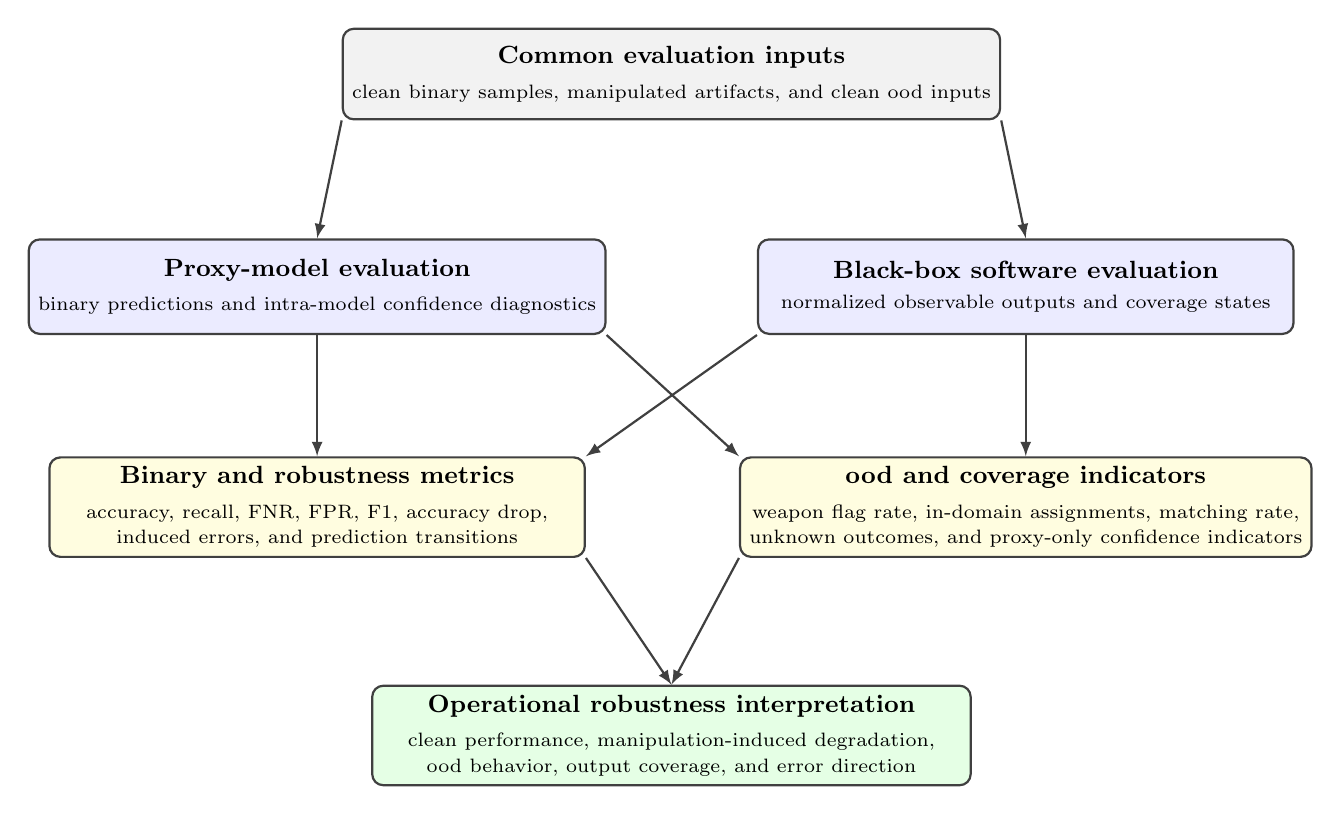
\begin{tikzpicture}[
>=latex,
font=\small,
block/.style={
rectangle,
rounded corners,
draw=black!75,
thick,
align=center,
minimum height=1.15cm,
minimum width=7.2cm,
fill=gray!10
},
eval/.style={
rectangle,
rounded corners,
draw=black!75,
thick,
align=center,
minimum height=1.20cm,
minimum width=6.8cm,
fill=blue!8
},
metric/.style={
rectangle,
rounded corners,
draw=black!75,
thick,
align=center,
minimum height=1.20cm,
minimum width=6.8cm,
fill=yellow!12
},
output/.style={
rectangle,
rounded corners,
draw=black!75,
thick,
align=center,
minimum height=1.20cm,
minimum width=7.6cm,
fill=green!10
},
arrow/.style={
->,
thick,
draw=black!75
}
]

\node[block] (inputs) at (0,0)
{\shortstack{
\textbf{Common evaluation inputs}\\[1mm]
\scriptsize clean binary samples, manipulated artifacts, and clean
\gls{ood} inputs
}};

\node[eval] (proxy) at (-4.5,-2.7)
{\shortstack{
\textbf{Proxy-model evaluation}\\[1mm]
\scriptsize binary predictions and intra-model confidence diagnostics
}};

\node[eval] (blackbox) at (4.5,-2.7)
{\shortstack{
\textbf{Black-box software evaluation}\\[1mm]
\scriptsize normalized observable outputs and coverage states
}};

\node[metric] (binary) at (-4.5,-5.5)
{\shortstack{
\textbf{Binary and robustness metrics}\\[1mm]
\scriptsize accuracy, recall, FNR, FPR, F1, accuracy drop,\\
\scriptsize induced errors, and prediction transitions
}};

\node[metric] (oodcoverage) at (4.5,-5.5)
{\shortstack{
\textbf{\gls{ood} and coverage indicators}\\[1mm]
\scriptsize weapon flag rate, in-domain assignments, matching rate,\\
\scriptsize unknown outcomes, and proxy-only confidence indicators
}};

\node[output] (interpretation) at (0,-8.4)
{\shortstack{
\textbf{Operational robustness interpretation}\\[1mm]
\scriptsize clean performance, manipulation-induced degradation,\\
\scriptsize \gls{ood} behavior, output coverage, and error direction
}};

\draw[arrow] (inputs.south west) -- (proxy.north);
\draw[arrow] (inputs.south east) -- (blackbox.north);

\draw[arrow] (proxy.south) -- (binary.north);
\draw[arrow] (proxy.south east) -- (oodcoverage.north west);

\draw[arrow] (blackbox.south west) -- (binary.north east);
\draw[arrow] (blackbox.south) -- (oodcoverage.north);

\draw[arrow] (binary.south east) -- (interpretation.north);
\draw[arrow] (oodcoverage.south west) -- (interpretation.north);

\end{tikzpicture}%
}
\caption[Metric framework]{Metric framework. Condition-specific binary,
robustness, \gls{ood}, and coverage indicators are computed across the
proxy-model and black-box evaluation levels and integrated only during the
operational interpretation}
\label{fig:methodology-metric-layers}
\end{figure}

The metrics do not replace human review or establish that a software system is
reliable across all forensic scenarios. Their function is to identify the
conditions under which automated support may fail to surface target-category
content, increase the review workload, or produce unstable or operationally
consequential outputs on manipulated or distributionally different inputs.


% ─────────────────────────────────────────────────────────────────────────────
\section{Explainability Approach}
\label{sec:methodology-explainability}
% ─────────────────────────────────────────────────────────────────────────────

The \gls{xai} component of the \gls{fairlab} methodology serves an exclusively
diagnostic and qualitative function. It complements quantitative robustness
metrics by supporting the examination of selected cases in which the behavior
of an inspectable proxy classification model is operationally or
methodologically relevant.

Explainability outputs are not treated as stand-alone evidence, definitive
explanations of algorithmic decisions, or demonstrations of model reliability.
Their purpose is to provide diagnostic information about the attribution
patterns associated with a selected model output and to support the formulation
of hypotheses regarding changes in model behavior across clean, adversarial,
anti-forensic, and \gls{ood} conditions.

In the present research design, the explainability analysis is restricted to
one selected fully inspectable proxy model. The adopted technique must therefore
be compatible with the model architecture, weights, preprocessing procedure,
and inference pipeline. Depending on the selected method, access may also be
required to gradients, intermediate activations, or other differentiable model
components.

The same internal attribution analysis cannot be applied directly to the
selected black-box or near-black-box software systems. Their internal model
architectures, gradients, representations, decision thresholds, and scoring
procedures are not accessible. Comparisons involving these systems are
therefore limited to their observable and normalized outputs. Such outputs must
not be interpreted as explanations of the internal decision processes that
produced them.

The explainability methodology adopts a case-study approach rather than an
aggregate evaluation strategy. Representative samples are selected according to
predefined diagnostic criteria. The objective is not to estimate model
performance from a limited number of visualizations, but to examine specific
behaviors that cannot be fully characterized through aggregate metrics alone.

Relevant case categories include:

\begin{itemize}
\item a correctly classified clean sample used as a qualitative reference;

\item a clean sample associated with an operationally relevant
classification error;

\item a high-confidence \gls{ood} assignment to an in-domain operational
class;

\item a clean-correct sample rendered incorrect by an anti-forensic
transformation;

\item a clean-correct sample rendered incorrect by a model-dependent
adversarial perturbation, particularly when the resulting prediction
retains high model confidence.
\end{itemize}

High-confidence criteria are applied only within the selected proxy model. They
serve as diagnostic case-selection indicators and must not be interpreted as
calibrated probabilities or compared directly with confidence values from other
architectures or software systems.

Table~\ref{tab:methodology-xai-case-selection} summarizes the diagnostic
function of these case categories.

\begin{table}[H]
\centering
\caption{Case-selection criteria for explainability analysis}
\label{tab:methodology-xai-case-selection}
\begin{tabularx}{\textwidth}{@{}L{4.4cm}X@{}}
\toprule
\textbf{Case category} &
\textbf{Diagnostic function} \\
\midrule

Correctly classified clean reference
&
Provide a qualitative reference for examining whether the attribution pattern
is associated with visually relevant regions under an unmanipulated condition.
\\

Clean classification error
&
Examine an error already present under the clean condition and determine
whether the attribution pattern appears localized, diffuse, partial, or
associated with contextual image regions. \\

High-confidence \gls{ood} assignment
&
Examine the attribution pattern associated with an in-domain assignment
produced for a distributionally different input. The assignment is treated as
an operational behavior rather than as an ordinary supervised error. \\

Anti-forensic induced error
&
Examine whether an operationally plausible image transformation is associated
with a change in the attribution pattern and the resulting predicted class. \\

Adversarially induced error
&
Examine the attribution pattern associated with an incorrect prediction
produced after a model-dependent adversarial perturbation, including cases in
which the model output remains highly confident. \\

\bottomrule
\end{tabularx}
\end{table}

Case selection must remain traceable to the corresponding prediction records,
source samples, experimental conditions, and model configurations. Each
explainability artifact should therefore be associated with the evaluated
sample, the model and checkpoint used for inference, the predicted class, the
reference operational class, the evaluation condition, and the rationale for
case selection.

The methodology does not prescribe a single explainability technique for every
possible implementation of the protocol. Gradient-based attribution,
activation-based visualization, local surrogate methods, and other
feature-attribution approaches may be considered, provided that their
assumptions and limitations are compatible with the selected model and the
research questions under examination. The specific technique and configuration
adopted in this thesis are reported in
Chapter~\ref{chap:implementation}.

The adopted explainability procedure should satisfy the following requirements:

\begin{itemize}
\item compatibility with the selected inspectable proxy model;
\item explicit documentation of the attribution target and reference
baseline, where required by the method;
\item reproducibility of the attribution procedure;
\item consistent application across the selected clean and manipulated
cases;
\item traceability to the model checkpoint, input sample, and prediction
record;
\item production of outputs that can be interpreted without being presented
as definitive causal explanations.
\end{itemize}

Attribution maps and related visualizations must be interpreted cautiously.
They characterize the relationship between input features and a selected model
output under the assumptions of the adopted explainability method. They do not
establish that the highlighted regions reproduce the model's internal
reasoning, nor do they demonstrate that the resulting prediction is correct,
reliable, or forensically valid.

When the adopted method provides completeness, approximation, or convergence
diagnostics, these quantities should be documented and considered during
interpretation. They constitute validation aids rather than automatic evidence
that an attribution is complete or reliable. No strict convergence claim should
be made unless it is supported by the recorded diagnostic values and the
adopted acceptance criterion.

The explainability analysis must also remain distinct from the quantitative
robustness assessment. Classification metrics measure the frequency, magnitude,
and direction of observed errors across the experimental corpus. Explainability
instead supports the qualitative examination of selected examples and the
interpretation of possible changes in attribution patterns.

Within the \gls{fairlab} protocol, \gls{xai} therefore acts as a supporting
diagnostic layer. It contributes to the interpretation of representative model
decisions and failure cases while preserving the distinction among technical
attribution, experimental robustness evaluation, and the evidentiary assessment
performed by a human forensic analyst.


% ─────────────────────────────────────────────────────────────────────────────
\section{Traceability and Reproducibility Controls}
\label{sec:methodology-traceability-controls}
% ─────────────────────────────────────────────────────────────────────────────

Traceability is a cross-cutting requirement of the entire \gls{fairlab}
protocol. It applies not only to dataset construction, but to every stage of the
experimental workflow, including technical preparation, human-in-the-loop
review, dataset freezing, partition generation, proxy-model training,
perturbation generation, bundle construction, black-box software evaluation,
metric computation, and \gls{xai} analysis.

Consistent with established \gls{df} principles, each processing step that
creates or modifies an experimental file must be documented so that the
relationships among the original sample, any derived artifact, the
corresponding model or software output, and the final experimental result can
be reconstructed
\cite{casey2011digital,nist2006guide,iso27037}.

The traceability framework relies on stable identifiers, integrity information,
structured provenance records, and explicit associations among experimental
inputs, derived artifacts, configurations, and outputs. Each sample must remain
identifiable throughout its complete lifecycle, even when its filename,
encoding, directory location, or visual representation changes.

The methodology distinguishes among four complementary traceability elements:

\begin{enumerate}
\item \textit{sample identity}, which establishes a stable reference to the
original image;

\item \textit{artifact lineage}, which records the relationship between an
original sample and any derived adversarial, anti-forensic, blind-bundle, or
explainability artifact;

\item \textit{experimental context}, which associates each input or derived
artifact with its reference operational assignment, partition, model
configuration, perturbation condition, and evaluation branch;

\item \textit{output provenance}, which connects model predictions,
software exports, normalization decisions, metrics, and qualitative case
studies to the corresponding evaluation input.
\end{enumerate}

Integrity verification should be based on cryptographic identifiers or other
mechanisms capable of detecting unintended changes to the experimental files.
The methodology does not prescribe a specific hashing algorithm. The selected
mechanism must nevertheless be documented and applied consistently across the
relevant stages of the pipeline.

Additional identifiers may be retained when required for interoperability with
selected black-box software systems. Such auxiliary identifiers must not
replace the primary integrity mechanism unless their security and
collision-resistance properties are appropriate for that role.

Traceability records should be progressive. Each stage should preserve the
identifiers inherited from the preceding stage and add only the information
required to describe the newly created artifact, configuration, or experimental
condition. This approach enables the lifecycle of each sample to be
reconstructed without relying exclusively on directory structures or
filenames.

Table~\ref{tab:methodology-traceability-artifacts} summarizes the principal
categories of traceability records required by the methodology.

\begin{table}[H]
\centering
\caption{Principal traceability records across the FAIRLab protocol}
\label{tab:methodology-traceability-artifacts}
\begin{tabularx}{\textwidth}{@{}L{4.2cm}X@{}}
\toprule
\textbf{Record category} &
\textbf{Role in traceability} \\
\midrule

Technical preparation records
&
Document sample identity, provenance, technical validity, and integrity
information for the candidate image pool. \\

Human-review records
&
Associate each candidate sample with its review status, operational assignment,
exclusion disposition, and supporting notes. \\

Frozen-dataset records
&
Define the stable experimental corpus and preserve the reference operational
assignments used in the subsequent phases. \\

Partition records
&
Associate each sample with its binary or \gls{ood} evaluation branch and, where
applicable, its experimental fold. \\

Model records
&
Document model architecture, training configuration, class mapping, checkpoint
identity, and the relationship between each checkpoint and its training
partitions. \\

Derived-artifact records
&
Link adversarial and anti-forensic artifacts to the corresponding clean sample,
generation condition, parameters, and model configuration when applicable. \\

Evaluation-bundle records
&
Map neutral blind identifiers to the corresponding source sample, reference
operational assignment, experimental condition, and integrity information. \\

Prediction and normalization records
&
Connect proxy-model predictions and observable software outputs to the evaluated
input and document any matching, recoding, or mapping decision. \\

Metric and explainability records
&
Associate quantitative results and qualitative case studies with the underlying
samples, model checkpoints, software configurations, and experimental
conditions. Explainability records refer only to the selected inspectable proxy
model. \\

\bottomrule
\end{tabularx}
\end{table}

The minimum traceability chain must make it possible to move in both directions:
from an original sample to its evaluation inputs, derived artifacts, and
experimental outputs, and from a reported result back to the exact input,
configuration, and processing conditions that produced it.

Figure~\ref{fig:methodology-traceability-chain} summarizes this general
traceability chain.

\begin{figure}[H]
\centering
\resizebox{0.96\textwidth}{!}{%
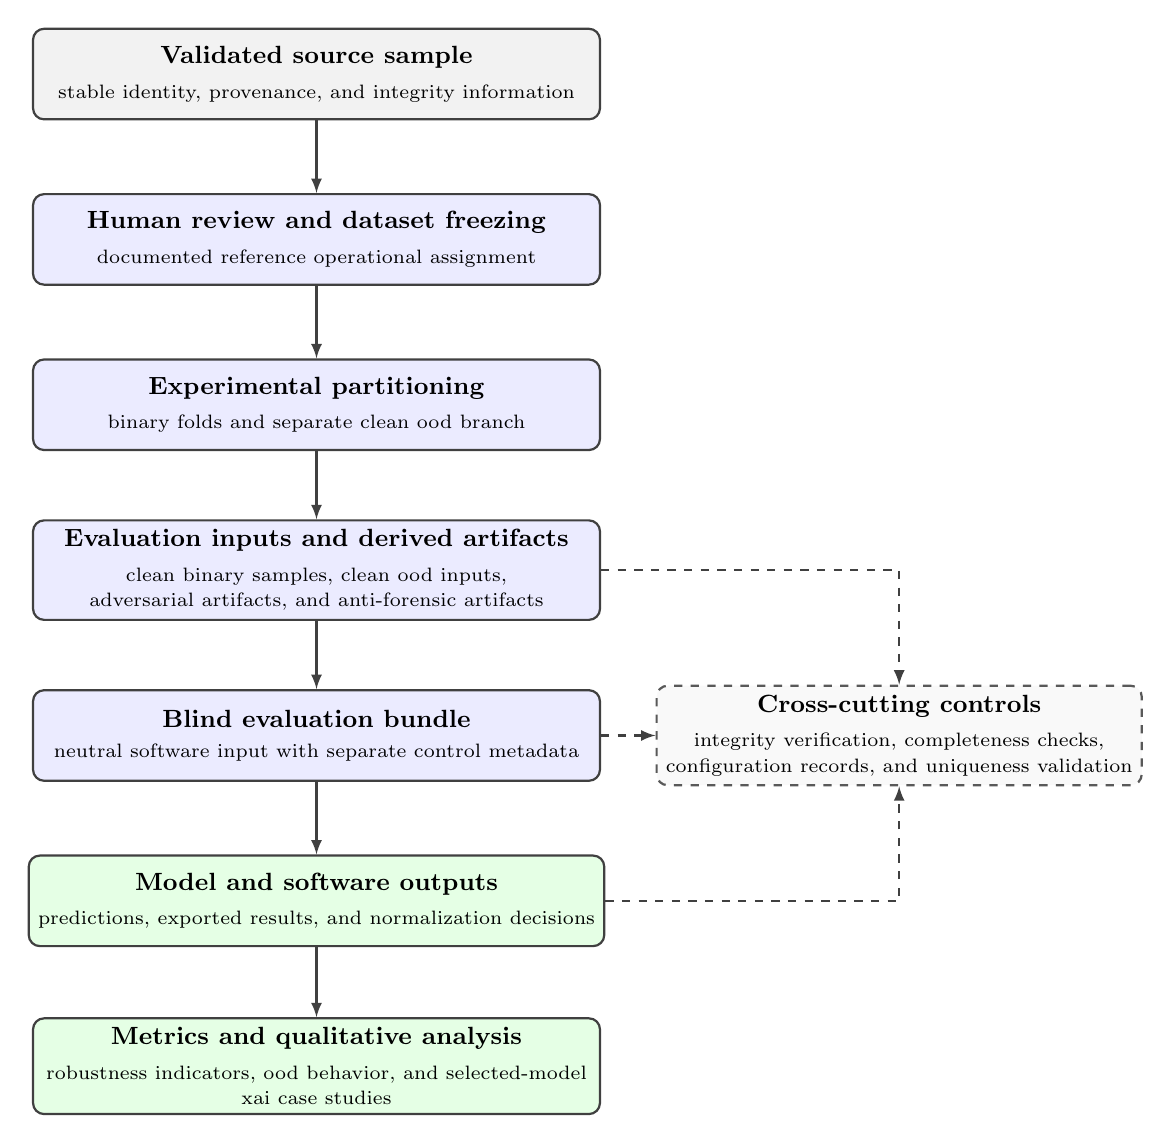
\begin{tikzpicture}[
>=latex,
font=\small,
block/.style={
rectangle,
rounded corners,
draw=black!75,
thick,
align=center,
minimum height=1.15cm,
minimum width=7.2cm,
fill=gray!10
},
process/.style={
rectangle,
rounded corners,
draw=black!75,
thick,
align=center,
minimum height=1.15cm,
minimum width=7.2cm,
fill=blue!8
},
output/.style={
rectangle,
rounded corners,
draw=black!75,
thick,
align=center,
minimum height=1.15cm,
minimum width=7.2cm,
fill=green!10
},
note/.style={
rectangle,
rounded corners,
draw=black!65,
dashed,
thick,
align=center,
minimum height=1.05cm,
minimum width=6.0cm,
fill=gray!5
},
arrow/.style={
->,
thick,
draw=black!75
},
dashedarrow/.style={
->,
thick,
dashed,
draw=black!75
}
]

\node[block] (source) at (0,0)
{\shortstack{
\textbf{Validated source sample}\\[1mm]
\scriptsize stable identity, provenance, and integrity information
}};

\node[process] (review) at (0,-2.1)
{\shortstack{
\textbf{Human review and dataset freezing}\\[1mm]
\scriptsize documented reference operational assignment
}};

\node[process] (partition) at (0,-4.2)
{\shortstack{
\textbf{Experimental partitioning}\\[1mm]
\scriptsize binary folds and separate clean \gls{ood} branch
}};

\node[process] (evaluationinputs) at (0,-6.3)
{\shortstack{
\textbf{Evaluation inputs and derived artifacts}\\[1mm]
\scriptsize clean binary samples, clean \gls{ood} inputs,\\
\scriptsize adversarial artifacts, and anti-forensic artifacts
}};

\node[process] (bundle) at (0,-8.4)
{\shortstack{
\textbf{Blind evaluation bundle}\\[1mm]
\scriptsize neutral software input with separate control metadata
}};

\node[output] (predictions) at (0,-10.5)
{\shortstack{
\textbf{Model and software outputs}\\[1mm]
\scriptsize predictions, exported results, and normalization decisions
}};

\node[output] (analysis) at (0,-12.6)
{\shortstack{
\textbf{Metrics and qualitative analysis}\\[1mm]
\scriptsize robustness indicators, \gls{ood} behavior, and selected-model\\
\scriptsize \gls{xai} case studies
}};

\node[note] (controls) at (7.4,-8.4)
{\shortstack{
\textbf{Cross-cutting controls}\\[1mm]
\scriptsize integrity verification, completeness checks,\\
\scriptsize configuration records, and uniqueness validation
}};

\draw[arrow] (source) -- (review);
\draw[arrow] (review) -- (partition);
\draw[arrow] (partition) -- (evaluationinputs);
\draw[arrow] (evaluationinputs) -- (bundle);
\draw[arrow] (bundle) -- (predictions);
\draw[arrow] (predictions) -- (analysis);

\draw[dashedarrow] (evaluationinputs.east) -| (controls.north);
\draw[dashedarrow] (bundle.east) -- (controls.west);
\draw[dashedarrow] (predictions.east) -| (controls.south);

\end{tikzpicture}%
}
\caption[Traceability chain across the FAIRLab protocol]{Traceability chain
across the FAIRLab protocol. Stable identifiers, provenance information,
integrity controls, and structured records preserve the relationships among
source samples, evaluation inputs, derived artifacts, observable outputs, and
final analyses}
\label{fig:methodology-traceability-chain}
\end{figure}

Reproducibility requires more than the availability of source code. The
experimental configuration must be documented in sufficient detail to recreate
the relevant processing conditions. This documentation should include the
dataset version, partitioning strategy, randomization controls, model
configuration, preprocessing rules, perturbation parameters, software version,
enabled functionality, normalization rules, and metric definitions.

Where randomness affects dataset partitioning, model initialization,
optimization, perturbation generation, or case selection, the relevant random
state or deterministic procedure must be recorded. Deterministic execution is
preferred when it does not conflict with the intended experimental design.

Model artifacts must be associated with the training partitions and
configuration that produced them. In fold-aware evaluation, the proxy-model
checkpoint used to evaluate a held-out binary sample, or to generate a
model-dependent adversarial artifact from that sample, must not have been
trained on the sample itself. This constraint reduces the risk of information
leakage and supports valid interpretation of the resulting robustness
measurements.

Generated adversarial and anti-forensic artifacts must preserve their
relationships with the corresponding clean inputs. Model-dependent adversarial
artifacts must additionally identify the relevant source model and
fold-specific checkpoint. This information is required to distinguish direct
source-model evaluation from cross-model and black-box transfer evaluation.

Model-agnostic adversarial-style and anti-forensic artifacts do not originate
from a designated source model. Their records must instead preserve the shared
generation condition and applied configuration so that responses can be
compared across proxy models and selected black-box software systems without
describing the comparison as transferability.

The blind evaluation of selected black-box software systems introduces an
additional traceability requirement. Experimental metadata must remain separate
from the software input during processing, but must remain available after
export to support input matching, normalization, and metric computation.

The separation between blind inputs and control metadata must itself be
verifiable. The evaluation records should demonstrate that reference
operational assignments, perturbation names, fold allocations, model
identifiers, and other controlled experimental descriptors were not exposed
through filenames, paths, directory structures, or accompanying control files
during software processing.

Automated consistency controls should verify, where applicable:

\begin{itemize}
\item correspondence between expected and generated artifacts;
\item uniqueness of stable and derived identifiers;
\item integrity of generated files;
\item absence of missing or unresolved paths;
\item consistency among source records, derived artifacts, and evaluation
outputs;
\item completeness of software exports and normalized predictions;
\item separation between blind inputs and experimental metadata.
\end{itemize}

These controls establish the technical coherence of the experimental workflow.
They do not demonstrate classification correctness or operational robustness.
Their purpose is to ensure that the reported results derive from the intended
inputs, artifacts, and configurations rather than from undocumented
substitutions, incomplete runs, or incorrect associations.

Traceability and reproducibility must also be considered within the limitations
of black-box evaluation. Selected software systems may change across versions,
and their internal models, thresholds, or processing logic may remain
unavailable. Accordingly, reproducibility in this context concerns the
documented external configuration, submitted inputs, observable outputs, and
normalization procedures rather than the inaccessible internal inference
process.

The protocol therefore combines procedural reproducibility with artifact-level
traceability. Procedural reproducibility documents how the experiment can be
repeated, whereas artifact-level traceability makes it possible to verify which
specific inputs, models, software configurations, and derived files contributed
to each reported result.

The concrete implementation of these controls is documented in
Chapter~\ref{chap:implementation}, whereas the corresponding experimental
outcomes are reported in Chapter~\ref{chap:results}.


















% ----------------- Chapter 5: Implementation and Experimental Setup ----------------------
% ─────────────────────────────────────────────────────────────────────────────
\chapter{Implementation and Experimental Setup}
\label{chap:implementation}
% ─────────────────────────────────────────────────────────────────────────────

This chapter documents the concrete implementation of the \gls{fairlab}
methodology introduced in Chapter~\ref{chap:methodology}. It describes how the
experimental protocol was instantiated through the preparation and freezing of
the image corpus, the generation of deterministic data partitions, the
training of fold-aware proxy models, the production of adversarial and
anti-forensic variants, and the construction of the forensic evaluation
bundle.

The chapter also reports the configurations adopted for the selected black-box
software systems, the procedures used to match and normalize their observable
outputs, and the technical controls introduced to preserve artifact identity,
provenance, integrity, and reproducibility. The implementation of the
explainability workflow and the generation of the consolidated evaluation
artifacts are documented as part of the same experimental pipeline.

The distinction between implementation and experimental evidence is maintained
throughout the chapter. The present chapter describes how the protocol was
realized and which technical artifacts were produced, whereas the quantitative
outcomes and their operational interpretation are reported separately in
Chapter~\ref{chap:results}. This separation prevents implementation choices,
software configurations, and data-management procedures from being conflated
with the measured robustness of the evaluated systems.


% ─────────────────────────────────────────────────────────────────────────────
\section{Experimental Workflow and Implementation Environment}
\label{sec:implementation-overview}
% ─────────────────────────────────────────────────────────────────────────────


% ─────────────────────────────────────────────────────────────────────────────
\section{Dataset Preparation and Organization}
\label{sec:implementation-dataset}
% ─────────────────────────────────────────────────────────────────────────────

\subsection{Technical Preparation and Source Consolidation}
\label{subsec:implementation-dataset-preparation}

\subsection{Review Documentation and Human-in-the-Loop Validation}
\label{subsec:implementation-human-review}

\subsection{Final Dataset Composition and Freezing}
\label{subsec:implementation-dataset-freezing}

\subsection{Dataset Partitioning and Fold Generation}
\label{subsec:implementation-split-generation}


% ─────────────────────────────────────────────────────────────────────────────
\section{Proxy-Model Implementation}
\label{sec:implementation-proxy-models}
% ─────────────────────────────────────────────────────────────────────────────

\subsection{Architectures and Preprocessing}
\label{subsec:implementation-architectures}

\subsection{Training Configuration and Fold-Aware Checkpoints}
\label{subsec:implementation-training}


% ─────────────────────────────────────────────────────────────────────────────
\section{Perturbation Implementation}
\label{sec:implementation-perturbations}
% ─────────────────────────────────────────────────────────────────────────────

\subsection{Adversarial Attack Implementation}
\label{subsec:implementation-adversarial}

\subsection{Anti-Forensic Transformation Implementation}
\label{subsec:implementation-antiforensic}


% ─────────────────────────────────────────────────────────────────────────────
\section{Forensic Evaluation Bundle Construction}
\label{sec:implementation-forensic-bundle}
% ─────────────────────────────────────────────────────────────────────────────


% ─────────────────────────────────────────────────────────────────────────────
\section{Black-Box Software Configuration and Output Normalization}
\label{sec:implementation-forensic-tools}
% ─────────────────────────────────────────────────────────────────────────────

\subsection{Magnet AXIOM and Magnet.AI}
\label{subsec:implementation-magnet}

\subsection{Magnet Griffeye and T3K CORE}
\label{subsec:implementation-griffeye}

\subsection{Excire Foto 2025}
\label{subsec:implementation-excire}

\subsection{Cellebrite Inseyets}
\label{subsec:implementation-cellebrite}

\subsection{Output Matching and Normalization}
\label{subsec:implementation-normalization}


% ─────────────────────────────────────────────────────────────────────────────
\section{Metric Computation and Explainability Implementation}
\label{sec:implementation-analysis}
% ─────────────────────────────────────────────────────────────────────────────

\subsection{Metric Computation and Evaluation Artifacts}
\label{subsec:implementation-metrics}

\subsection{Integrated Gradients Implementation}
\label{subsec:implementation-explainability}


% ─────────────────────────────────────────────────────────────────────────────
\section{Traceability, Integrity, and Reproducibility Controls}
\label{sec:implementation-traceability}
% ─────────────────────────────────────────────────────────────────────────────

% ----------------- Chapter 6: Experimental Results ----------------------
% ─────────────────────────────────────────────────────────────────────────────
\chapter{Experimental Results and Operational Robustness Analysis}
\label{chap:results}
% ─────────────────────────────────────────────────────────────────────────────

This chapter presents the quantitative outcomes obtained from the
implementation documented in Chapter~\ref{chap:implementation} and interprets
them according to the methodological framework defined in
Chapter~\ref{chap:methodology}. The analysis focuses on the operational
robustness of \gls{ai}-based systems for automated image classification and
triage in forensic contexts.

A central feature of the evaluation is the parallel analysis of two
complementary system levels. The first comprises the transparent proxy models
defined in Section~\ref{subsec:implementation-architectures}, for which
predictions, maximum predicted-class probabilities, confusion matrices, and
internal attribution information are available. The second comprises the
selected black-box software systems, whose behavior is assessed exclusively
through observable and normalized outputs.

Both evaluation levels operate on the same frozen source population. The
1\,000 clean binary images and 500 clean \gls{ood} images constitute the common
source corpus, whereas 10\,000 adversarial and anti-forensic artifacts are
derived exclusively from the binary subset. The resulting comparison is
therefore based on the same underlying samples and experimental conditions,
while preserving the distinction between transparent model evaluation and
operational black-box assessment.

The purpose of the chapter is not to construct an absolute ranking among
heterogeneous systems or to reduce the study to a conventional
\gls{advml} benchmark. The systems differ in architecture, output semantics,
configuration, operational scope, and degree of transparency. Their results
are therefore interpreted from a forensic perspective, with particular
attention to false negatives on the firearm-oriented target category, false
positives on \texttt{non\_weapon} content, closed-set assignments of
\gls{ood} inputs, degradation under manipulated conditions, and the continued
need for human review
\cite{costantini2019digital,sanna2024preliminary,sanna2025pixelperfect}.

% ─────────────────────────────────────────────────────────────────────────────
\section{Experimental Evaluation Scope and Completeness}
\label{sec:results-scope}
% ─────────────────────────────────────────────────────────────────────────────

The experimental results cover the complete population generated through the
frozen implementation described in Chapter~\ref{chap:implementation}. The
common corpus contains 11\,500 logical experimental inputs, comprising clean
images and derived perturbed artifacts:

\begin{equation}
\begin{aligned}
N_{\mathrm{bundle}}
&=
1\,000\ \text{clean binary inputs}
+
500\ \text{\glsentryshort{ood} inputs}
\\
&\quad
+
5\,000\ \text{adversarial artifacts}
+
5\,000\ \text{anti-forensic artifacts}
\\
&=
11\,500.
\end{aligned}
\end{equation}

The proxy-model and black-box evaluations use different output
representations but cover the same experimental conditions. Each clean binary
input or perturbed binary artifact is evaluated by all three proxy
architectures through the checkpoint associated with its assigned fold.

The \gls{ood} branch follows a different proxy-model evaluation protocol. Each
of the 500 unique \gls{ood} images is evaluated by all five fold-specific
checkpoints of each architecture. The resulting 7\,500 prediction rows
therefore represent repeated checkpoint responses to 500 unique images and
must not be interpreted as 7\,500 independent \gls{ood} samples.

The black-box evaluation comprises four software families and six normalized
operational configurations. Magnet AXIOM/Magnet.AI, Griffeye/T3K CORE, and
Cellebrite Inseyets each contribute one configuration, whereas the D20, D50,
and D80 Excire Foto 2025 settings are retained as three separate
configurations. Each configuration produces one normalized decision for every
item in the 11\,500-file forensic evaluation bundle.

Table~\ref{tab:results-evaluation-completeness} summarizes the completeness of
the result population.

\begin{table}[H]
\centering
\small
\renewcommand{\arraystretch}{1.15}
\setlength{\tabcolsep}{5pt}
\caption{Completeness of the experimental result population}
\label{tab:results-evaluation-completeness}
\begin{tabularx}{0.96\textwidth}{@{}l r X@{}}
\toprule
\textbf{Result layer} &
\textbf{Records} &
\textbf{Coverage} \\
\midrule

Proxy-model predictions
&
40\,500
&
3\,000 clean predictions, 7\,500 fold-specific \gls{ood} responses, and
30\,000 predictions on adversarial and anti-forensic artifacts; no recorded
inference errors. \\

Normalized black-box decisions
&
69\,000
&
Six normalized configurations evaluated on all 11\,500 bundle items, with no
missing bundle-level decision. \\

Proxy binary-condition metrics
&
33
&
Three clean architecture-level rows and 30 architecture--perturbation
combinations. \\

Proxy robustness comparisons
&
30
&
Clean-to-perturbed comparisons for three architectures and ten perturbation
conditions. \\

Proxy \gls{ood} summaries
&
3
&
One fold-aggregated \gls{ood} record for each proxy architecture. \\

Black-box software metrics
&
186
&
Thirty-one aggregation records for each of the six normalized black-box
configurations. \\

Explainability cases
&
5
&
One representative case for each predefined diagnostic category, associated
with 20 thesis-level visual assets. \\

\bottomrule
\end{tabularx}
\end{table}

Binary accuracy, precision, recall, F1-score, \gls{fpr}, and \gls{fnr} are
computed exclusively on samples whose reference operational assignment is
\texttt{weapon} or \texttt{non\_weapon}. The \gls{ood} branch remains
separate and is analyzed through the proportion of inputs assigned to the
\texttt{weapon} class and, for the proxy models, through architecture-specific
maximum-probability indicators.

Accuracy drop, induced-error counts, directional error transitions, and the
confusion-matrix layout follow the definitions established in
Section~\ref{sec:methodology-evaluation-metrics}. Positive accuracy-drop values
indicate degradation relative to the clean baseline, whereas negative values
indicate a condition-specific increase in accuracy that must not be interpreted
as evidence of general robustness.

The clean-correct-to-incorrect transition rate is interpreted as attack success
rate only for the four model-dependent adversarial attacks: \gls{fgsm}, One
Pixel, Sigma-Zero, and SuperDeepFool. For Color Shift and the five
anti-forensic transformations, the same numerical transition is interpreted as
an induced-error rate rather than as adversarial or transfer success.

Maximum predicted-class probabilities are available only for the transparent
proxy models. They are retained as intra-model diagnostic indicators and are
not interpreted as calibrated probabilities directly comparable across
architectures. The selected black-box software systems do not expose
homogeneous numerical uncertainty measures; consequently, their comparison is
based on normalized observable decisions rather than cross-system confidence
scores.

% ─────────────────────────────────────────────────────────────────────────────
\section{Clean Baseline Performance}
\label{sec:results-clean-baseline}
% ─────────────────────────────────────────────────────────────────────────────

Evaluation on clean inputs establishes the nominal baseline against which
behavior under \gls{ood}, adversarial, and anti-forensic conditions is
subsequently assessed. The three proxy architectures were evaluated on the
frozen binary subset of 1\,000 images, comprising 500
\texttt{weapon} and 500 \texttt{non\_weapon} samples.

The positive class is \texttt{weapon}, and the negative class is
\texttt{non\_weapon}. A false negative therefore corresponds to a
\texttt{weapon} image classified as \texttt{non\_weapon}, whereas a false
positive corresponds to a \texttt{non\_weapon} image classified as
\texttt{weapon}.

Table~\ref{tab:results-clean-baseline-metrics} reports the principal clean
binary metrics. In addition to accuracy, balanced accuracy, macro-averaged
metrics, and class-specific performance for \texttt{weapon}, the table includes
the mean maximum predicted-class probability. This value is retained only as
an architecture-specific diagnostic of the output distribution and is not
interpreted as a calibrated confidence measure.

\begin{table}[H]
\centering
\scriptsize
\setlength{\tabcolsep}{2.3pt}
\renewcommand{\arraystretch}{1.15}
\caption{Clean performance of the proxy models on the binary subset}
\label{tab:results-clean-baseline-metrics}
\begin{tabularx}{\textwidth}{@{}l *{11}{>{\centering\arraybackslash}X}@{}}
\toprule
\textbf{Model} &
\textbf{Acc.} &
\textbf{Bal.} &
\textbf{M-P} &
\textbf{M-R} &
\textbf{M-F1} &
\textbf{P\textsubscript{w}} &
\textbf{R\textsubscript{w}} &
\textbf{F1\textsubscript{w}} &
\textbf{Max-P} &
\textbf{\acrshort{fpr}} &
\textbf{\acrshort{fnr}} \\
\midrule

EfficientNet-B0
& 0.978
& 0.978
& 0.978
& 0.978
& 0.978
& 0.972
& 0.984
& 0.978
& 0.979
& 0.028
& 0.016 \\

ResNet18
& 0.964
& 0.964
& 0.964
& 0.964
& 0.964
& 0.958
& 0.970
& 0.964
& 0.974
& 0.042
& 0.030 \\

\acrshort{clip}
& 0.927
& 0.927
& 0.933
& 0.927
& 0.927
& 0.881
& 0.988
& 0.931
& 0.559
& 0.134
& 0.012 \\

\bottomrule
\end{tabularx}

\vspace{0.4em}
\footnotesize
\textit{Note.} \textit{Bal.} indicates balanced accuracy; \textit{M-P},
\textit{M-R}, and \textit{M-F1} indicate macro-precision, macro-recall, and
macro-F1, respectively; \(P_w\), \(R_w\), and \(F1_w\) indicate precision,
recall, and F1-score for the \texttt{weapon} class. \textit{Max-P} indicates
the mean maximum predicted-class probability and is reported only as an
intra-model diagnostic indicator.
\end{table}

EfficientNet-B0 achieves the strongest overall clean-condition performance,
with an accuracy and macro-F1 of 0.978. Its \texttt{weapon} recall is 0.984,
corresponding to an \gls{fnr} of 0.016, while its \gls{fpr} is 0.028. Its mean
maximum predicted-class probability is 0.979.

ResNet18 shows slightly lower but still high clean-condition performance, with
an accuracy and macro-F1 of 0.964. Its \texttt{weapon} recall is 0.970, its
\gls{fnr} is 0.030, and its \gls{fpr} is 0.042. The corresponding mean maximum
predicted-class probability is 0.974.

The \gls{clip}-based proxy exhibits a different operational profile. Its
overall accuracy and macro-F1 are 0.927, lower than those of the two
fully fine-tuned \glspl{cnn}. However, it achieves the highest
\texttt{weapon} recall, at 0.988, and the lowest \gls{fnr}, at 0.012. This
reduction in missed \texttt{weapon} samples is accompanied by an
\gls{fpr} of 0.134, substantially higher than those of EfficientNet-B0 and
ResNet18.

The mean maximum predicted-class probability of the \gls{clip}-based proxy is
0.559. This value must not be compared directly with the corresponding values
of the convolutional architectures because the probability outputs are not
calibrated across models. Within the \gls{clip}-based proxy, it indicates that
the strong tendency to assign inputs to the \texttt{weapon} class does not
generally coincide with maximum probabilities close to one.

This behavior is not the result of zero-shot classification. In the adopted
implementation, \gls{clip} serves as a pretrained and frozen visual encoder
connected to a supervised binary classification head trained on the same
frozen binary task. Its error profile must therefore be attributed to the
combination of the pretrained visual representation and the learned binary
decision head rather than to the original image--text similarity interface.

Table~\ref{tab:results-clean-confusion-matrices} reports the aggregate
confusion-matrix components for the three proxy models. The layout is:

\[
\mathbf{C}
=
\begin{bmatrix}
\glsentryshort{tn} & \glsentryshort{fp} \\
\glsentryshort{fn} & \glsentryshort{tp}
\end{bmatrix}.
\]

\begin{table}[H]
\centering
\caption{Clean confusion matrices of the proxy models}
\label{tab:results-clean-confusion-matrices}
\begin{tabular}{@{}l r r r r@{}}
\toprule
\textbf{Model} &
\textbf{\gls{tn}} &
\textbf{\gls{fp}} &
\textbf{\gls{fn}} &
\textbf{\gls{tp}} \\
\midrule

EfficientNet-B0
& 486
& 14
& 8
& 492 \\

ResNet18
& 479
& 21
& 15
& 485 \\

\gls{clip}
& 433
& 67
& 6
& 494 \\

\bottomrule
\end{tabular}
\end{table}

The same error distributions are visualized in
Figure~\ref{fig:results-clean-confusion-matrices}. EfficientNet-B0 minimizes
the total number of errors, producing 22 incorrect decisions. ResNet18 produces
36 errors and maintains an intermediate profile. The \gls{clip}-based proxy
produces 73 errors, but only six of them are false negatives; the remaining 67
are false positives.

\begin{figure}[htbp]
\centering

\begin{minipage}{0.48\textwidth}
\centering
\small EfficientNet-B0

\vspace{0.2em}
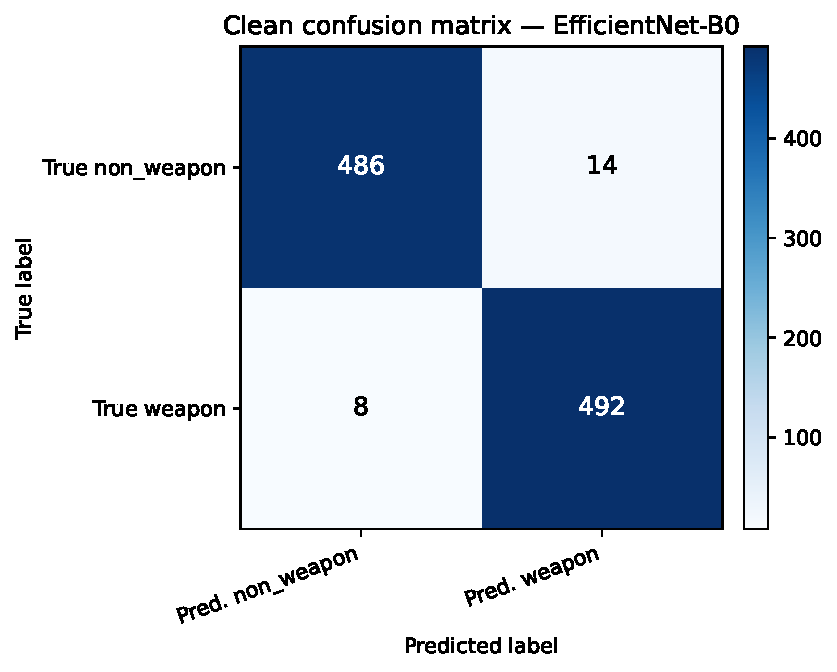
\includegraphics[width=\linewidth]
{images/fig_clean_confusion_matrix_efficientnet_b0.pdf}
\end{minipage}
\hfill
\begin{minipage}{0.48\textwidth}
\centering
\small ResNet18

\vspace{0.2em}
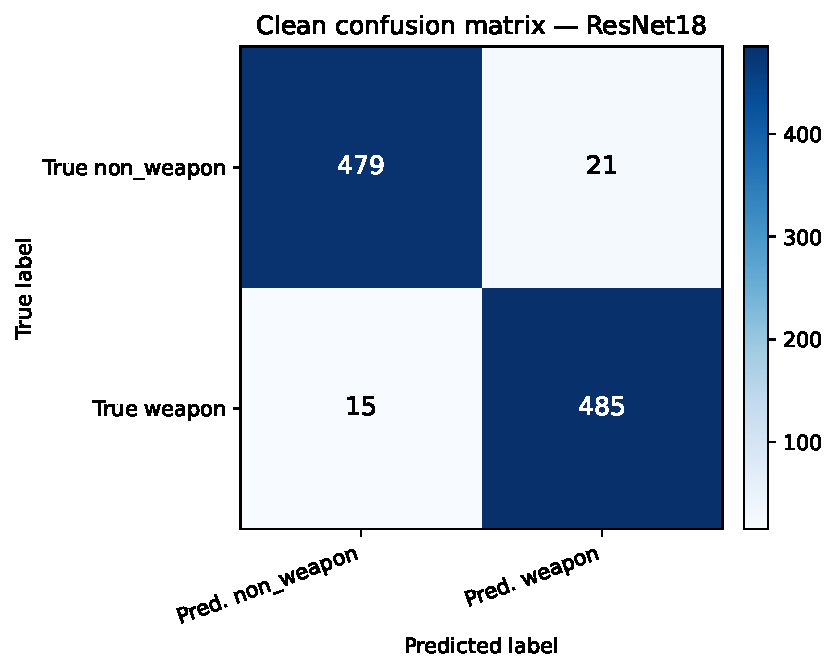
\includegraphics[width=\linewidth]
{images/fig_clean_confusion_matrix_resnet18.pdf}
\end{minipage}

\vspace{0.8em}

\begin{minipage}{0.58\textwidth}
\centering
\small \acrshort{clip}

\vspace{0.2em}
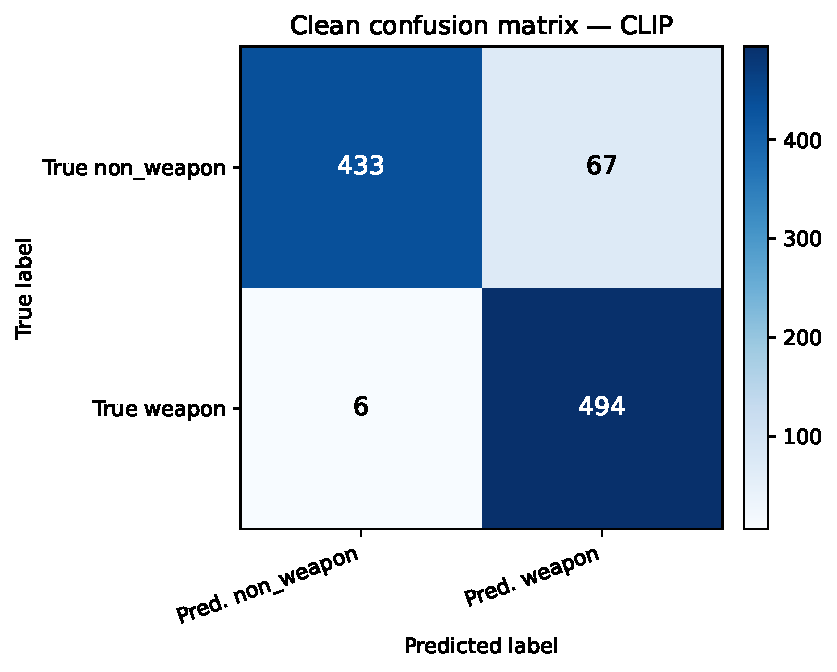
\includegraphics[width=\linewidth]
{images/fig_clean_confusion_matrix_clip.pdf}
\end{minipage}

\caption{Clean confusion matrices of the three proxy models on the binary
subset}
\label{fig:results-clean-confusion-matrices}
\end{figure}

From a forensic-triage perspective, the most consequential distinction concerns
the direction of the errors. EfficientNet-B0 provides the strongest overall
balance, with eight false negatives and 14 false positives. ResNet18 produces
15 false negatives and 21 false positives. The \gls{clip}-based proxy reduces
false negatives to six but increases false positives to 67.

The clean comparison therefore cannot be interpreted solely through aggregate
accuracy. A lower false-negative rate may reduce the risk of failing to flag
firearm-oriented content, but a higher false-positive rate increases the volume
of irrelevant material presented for human review. Conversely, minimizing the
review workload must not be achieved by accepting an operationally
unacceptable number of missed target images.

Overall, all three proxy architectures achieve high performance under clean
conditions, but they expose distinct operational tradeoffs among target-class
recall, false-negative risk, false-positive workload, and model-specific output
distributions. These differences provide the necessary baseline for evaluating
whether the same profiles remain stable under \gls{ood}, adversarial, and
anti-forensic conditions.

% ─────────────────────────────────────────────────────────────────────────────
\section{\texorpdfstring{\gls{ood}}{Out-of-Distribution} Behavior}
\label{sec:results-ood}
% ─────────────────────────────────────────────────────────────────────────────

The \gls{ood} evaluation examines the behavior of the three proxy architectures
on the separate 500-image \gls{ood} branch. As established in
Chapter~\ref{chap:methodology}, these images are not treated as a third
supervised class and do not contribute to binary accuracy, precision, recall,
or confusion-matrix counts.

The analysis instead characterizes how inputs outside the frozen binary
distribution are forced into one of the two available closed-set operational
classes
\cite{hendrycks2017baseline,liang2018odin,fort2021exploring}.

Each of the 500 unique \gls{ood} images was evaluated by all five
fold-specific checkpoints of each proxy architecture:

\begin{equation}
500\ \text{unique \glsentryshort{ood} images}
\times
5\ \text{fold-specific checkpoints}
=
2\,500\ \text{responses per architecture}.
\end{equation}

The resulting responses are not independent images. They represent five
fold-specific model outputs for each unique \gls{ood} input. The reported
counts and rates therefore characterize checkpoint-response behavior rather
than unique-image-level classification frequency.

Two principal indicators are considered:

\begin{itemize}
\item the \emph{weapon assignment rate}, defined as the proportion of the
2\,500 responses assigned to \texttt{weapon};

\item the \emph{high-maximum-probability rate}, defined as the proportion of
responses whose maximum predicted-class probability is at least 0.90.
\end{itemize}

Neither indicator represents supervised correctness because the \gls{ood}
inputs have no binary reference assignment.

Table~\ref{tab:results-ood-behavior} reports the fold-aggregated results.

\begin{table}[H]
\centering
\scriptsize
\setlength{\tabcolsep}{3.5pt}
\renewcommand{\arraystretch}{1.15}
\caption{Fold-aggregated behavior of the proxy models on \gls{ood} inputs}
\label{tab:results-ood-behavior}
\begin{tabular}{@{}l r r r r r r r@{}}
\toprule
\textbf{Model} &
\textbf{Responses} &
\textbf{\shortstack{Weapon\\responses}} &
\textbf{\shortstack{Non-weapon\\responses}} &
\textbf{W-rate} &
\textbf{Max-P} &
\textbf{HP-count} &
\textbf{HP-rate} \\
\midrule

EfficientNet-B0
& 2\,500
& 924
& 1\,576
& 0.3696
& 0.8505
& 1\,252
& 0.5008 \\

ResNet18
& 2\,500
& 1\,094
& 1\,406
& 0.4376
& 0.8896
& 1\,617
& 0.6468 \\

\acrshort{clip}
& 2\,500
& 2\,089
& 411
& 0.8356
& 0.5358
& 0
& 0.0000 \\

\bottomrule
\end{tabular}

\vspace{0.4em}
\footnotesize
\textit{Note.} \textit{W-rate} indicates the proportion of fold-specific
responses assigned to \texttt{weapon}; \textit{Max-P} indicates the mean
maximum predicted-class probability; \textit{HP-count} indicates the number of
responses whose maximum probability is at least 0.90; and \textit{HP-rate}
indicates the corresponding proportion over the 2\,500 responses. Each total
comprises five checkpoint responses for each of the 500 unique \gls{ood}
images.
\end{table}

The \gls{clip}-based proxy exhibits the strongest tendency to assign
\gls{ood} inputs to the firearm-oriented class. It produces 2\,089
\texttt{weapon} responses, corresponding to a weapon assignment rate of
0.8356. However, its mean maximum predicted-class probability is only 0.5358,
and none of its 2\,500 responses reaches the threshold of 0.90.

The zero high-maximum-probability rate must therefore not be interpreted as an
absence of \texttt{weapon} assignments. Instead, the \gls{clip}-based proxy
frequently selects \texttt{weapon} while producing output probabilities close
to the central region of the binary output range. This combination indicates a
strong directional assignment tendency without high maximum-probability
responses under the adopted threshold.

EfficientNet-B0 and ResNet18 assign lower proportions of the \gls{ood}
responses to \texttt{weapon}. EfficientNet-B0 produces 924 such responses,
corresponding to a rate of 0.3696, whereas ResNet18 produces 1\,094, for a rate
of 0.4376.

Their model-specific output distributions nevertheless contain substantially
more responses above the 0.90 threshold. EfficientNet-B0 produces 1\,252
high-maximum-probability responses, corresponding to a rate of 0.5008.
ResNet18 produces 1\,617, corresponding to the highest rate among the three
architectures, at 0.6468.

Figure~\ref{fig:results-ood-weapon-rate-confidence} compares the weapon
assignment rate, mean maximum predicted-class probability, and
high-maximum-probability rate.

\begin{figure}[H]
\centering
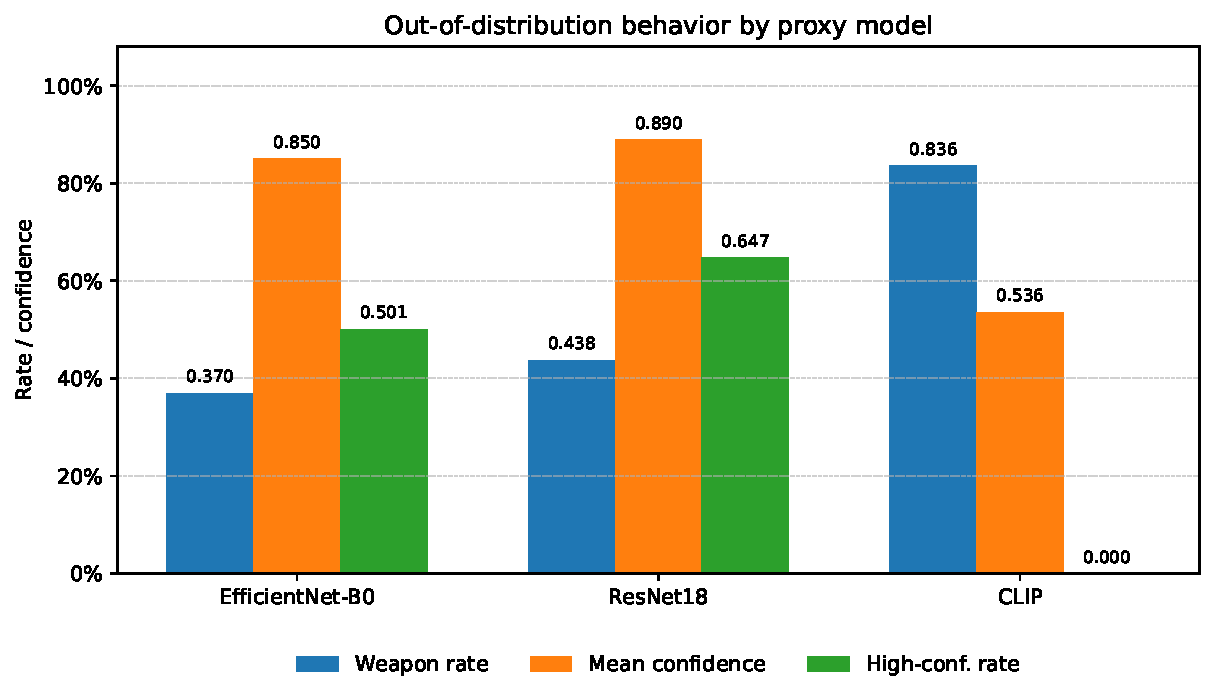
\includegraphics[width=0.95\textwidth]
{images/fig_ood_weapon_rate_and_confidence.pdf}
\caption{Weapon assignment rate and maximum predicted-class probability
indicators on \gls{ood} inputs}
\label{fig:results-ood-weapon-rate-confidence}
\end{figure}

The figure highlights that weapon assignment frequency and maximum-probability
behavior represent distinct dimensions of the closed-set response. The
\gls{clip}-based proxy exhibits the highest weapon assignment rate but the
lowest mean maximum probability and no responses above the 0.90 threshold.
ResNet18 exhibits the highest high-maximum-probability rate despite assigning
fewer responses to \texttt{weapon}. EfficientNet-B0 presents an intermediate
profile for both indicators.

These values are architecture-specific and must not be used to construct a
cross-model probability or uncertainty ranking. The output probabilities were
not calibrated across architectures, and the same numerical value may not
represent the same degree of uncertainty for EfficientNet-B0, ResNet18, and the
\gls{clip}-based proxy.

Figure~\ref{fig:results-ood-confidence-distribution} presents the complete
distribution of maximum predicted-class probabilities for the three
architectures.

\begin{figure}[H]
\centering
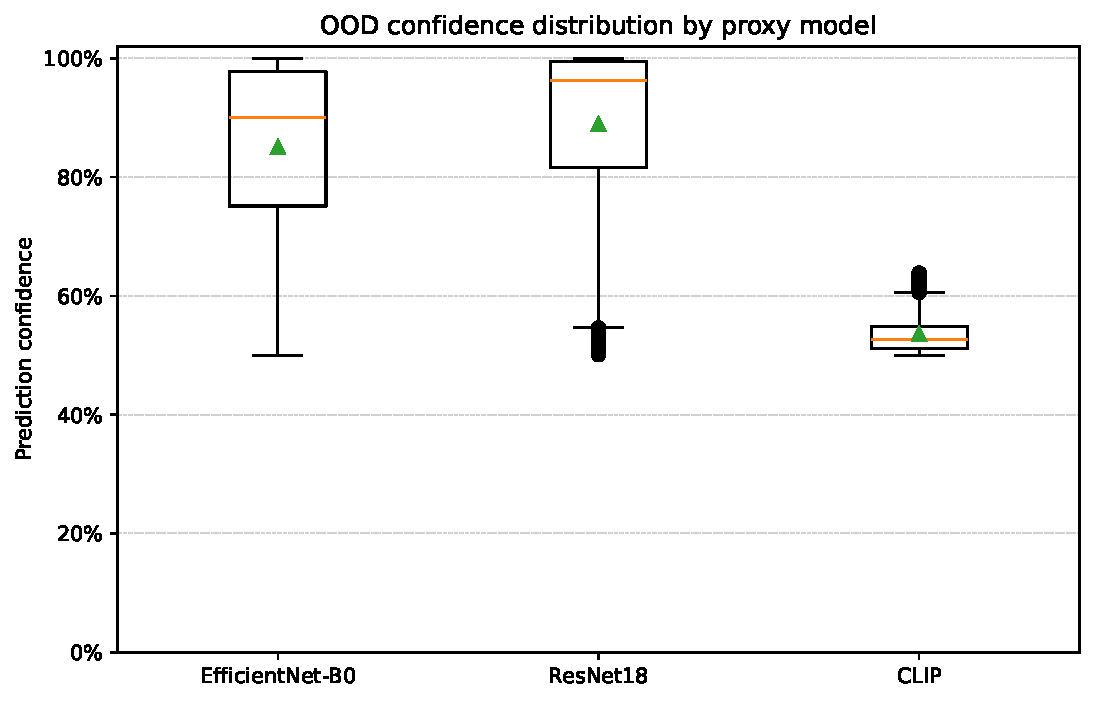
\includegraphics[width=0.95\textwidth]
{images/fig_ood_confidence_distribution.pdf}
\caption{Distribution of maximum predicted-class probabilities on
\gls{ood} inputs for each proxy architecture}
\label{fig:results-ood-confidence-distribution}
\end{figure}

The distributional view confirms that the responses of the \gls{clip}-based
proxy remain below the predefined 0.90 threshold, whereas EfficientNet-B0 and
ResNet18 produce substantial populations above it. This difference does not
establish that one architecture is intrinsically more reliable on
out-of-distribution content. It characterizes the architecture-specific score
profiles produced when all inputs must be assigned to one of two closed-set
classes.

From a forensic perspective, a \texttt{weapon} assignment on the \gls{ood}
branch is not a false positive in the supervised binary sense. The input has no
\texttt{weapon} or \texttt{non\_weapon} reference assignment. Nevertheless,
such an output may still affect triage by increasing the quantity of unrelated
material prioritized for review.

Conversely, a high maximum predicted-class probability on an \gls{ood} input
does not demonstrate that the assignment is semantically valid. It indicates
only that the corresponding proxy architecture produced a strongly peaked
closed-set output for material outside the frozen binary evaluation
distribution.

The \gls{ood} results therefore identify two operationally relevant but
separate behaviors:

\begin{itemize}
\item the tendency to route distributionally different material toward the
firearm-oriented review category;

\item the tendency to produce high maximum predicted-class probabilities for
forced closed-set assignments.
\end{itemize}

Both behaviors can influence prioritization and analyst workload. Neither can
be treated as stand-alone evidence, supervised correctness, or calibrated
uncertainty, and both remain subject to human verification
\cite{guo2017calibration,nist2023airmf}.

% ─────────────────────────────────────────────────────────────────────────────
\section{Anti-Forensic Robustness}
\label{sec:results-antiforensic}
% ─────────────────────────────────────────────────────────────────────────────

The anti-forensic evaluation examines the stability of the proxy models under
five deterministic, model-agnostic image transformations. These conditions do
not require access to model parameters, gradients, logits, or decision
thresholds. They represent operations compatible with ordinary image
circulation and processing, although the same transformations may also be
applied intentionally to alter observable image characteristics
\cite{stamm2010anti,yaacoub2021digital,hendrycks2019benchmarking}.

The evaluated conditions comprise JPEG recompression, downsampling followed by
resizing to the original dimensions, Gaussian blurring, histogram
modification, and contrast stretching. Their operational relevance derives
from the fact that they may occur during compression, platform-mediated
sharing, editing, conversion, or deliberate anti-forensic manipulation.

For each architecture and transformation, performance is compared with the
corresponding clean baseline. Accuracy drop is defined as:

\begin{equation}
\Delta_{\mathrm{acc}}
=
\mathrm{Acc}_{\mathrm{clean}}
-
\mathrm{Acc}_{\mathrm{transformed}}.
\end{equation}

Positive values indicate lower aggregate accuracy under the transformed
condition. A value of zero indicates unchanged aggregate accuracy, whereas a
negative value indicates higher accuracy on the specific transformed
population.

A zero or negative accuracy drop must not be interpreted as evidence that the
transformation introduced no adverse decisions. Aggregate accuracy may remain
unchanged or increase when some clean-condition errors are corrected while
other initially correct samples become incorrect. For this reason, accuracy
drop is examined together with the induced-error count, induced-error rate, and
direction of the clean-correct-to-incorrect transitions.

Table~\ref{tab:results-antiforensic-robustness} reports transformed accuracy and
accuracy drop for all architecture--transformation combinations.

\begin{table}[H]
\centering
\scriptsize
\setlength{\tabcolsep}{3.3pt}
\renewcommand{\arraystretch}{1.15}
\caption{Accuracy and accuracy drop under anti-forensic transformations}
\label{tab:results-antiforensic-robustness}
\begin{tabular}{@{}l r r r r r r@{}}
\toprule
\textbf{Transformation} &
\textbf{\gls{clip} acc.} &
\textbf{Drop} &
\textbf{EffNet acc.} &
\textbf{Drop} &
\textbf{ResNet acc.} &
\textbf{Drop} \\
\midrule

\gls{jpegrecompression}
& 0.925
& 0.002
& 0.976
& 0.002
& 0.964
& 0.000 \\

\gls{resampleresize}
& 0.929
& -0.002
& 0.976
& 0.002
& 0.963
& 0.001 \\

\gls{gaussianblur}
& 0.934
& -0.007
& 0.965
& 0.013
& 0.959
& 0.005 \\

\gls{histogrammodification}
& 0.925
& 0.002
& 0.973
& 0.005
& 0.934
& 0.030 \\

\gls{contraststretching}
& 0.927
& 0.000
& 0.974
& 0.004
& 0.963
& 0.001 \\

\bottomrule
\end{tabular}

\vspace{0.4em}
\footnotesize
\textit{Note.} Drop is computed as clean accuracy minus transformed accuracy.
Positive values indicate aggregate degradation, zero indicates unchanged
aggregate accuracy, and negative values indicate a condition-specific increase.
None of these values alone establishes the absence or presence of newly induced
errors.
\end{table}

Figure~\ref{fig:results-antiforensic-accuracy-drop-heatmap} presents the same
comparison as a heatmap.

\begin{figure}[H]
\centering
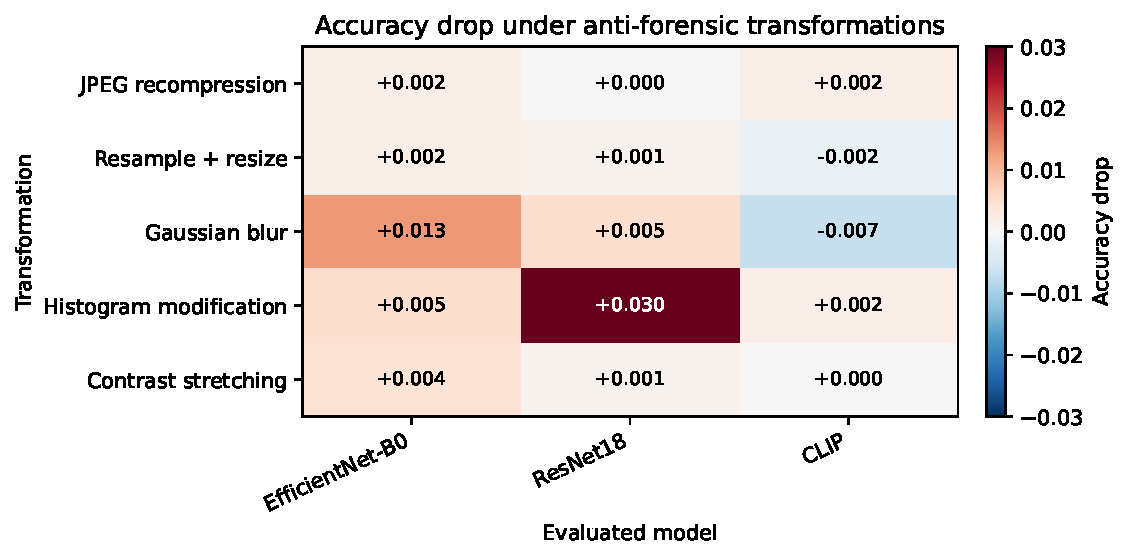
\includegraphics[width=0.88\textwidth]
{images/fig_anti_forensic_accuracy_drop_heatmap.pdf}
\caption{Accuracy drop of the proxy models under anti-forensic transformations}
\label{fig:results-antiforensic-accuracy-drop-heatmap}
\end{figure}

The aggregate results indicate that the five transformations produce smaller
accuracy variations than the strongest model-dependent adversarial attacks
examined in Section~\ref{sec:results-adversarial}. This relative difference
does not make the anti-forensic effects operationally negligible. Even limited
aggregate degradation may correspond to newly missed target-category images.

EfficientNet-B0 remains above 0.965 accuracy under every transformation.
Gaussian Blur produces its largest degradation, reducing accuracy from 0.978
to 0.965 and yielding an accuracy drop of 0.013. Histogram Modification is the
second most influential condition for this model, with an accuracy of 0.973 and
a drop of 0.005.

ResNet18 is most affected by Histogram Modification. Its accuracy decreases
from 0.964 to 0.934, corresponding to the largest anti-forensic accuracy drop
observed across the three architectures, at 0.030. Gaussian Blur produces a
smaller reduction to 0.959, corresponding to a drop of 0.005. JPEG
Recompression leaves aggregate accuracy unchanged at 0.964.

The \gls{clip}-based proxy exhibits small aggregate variations across the five
conditions. JPEG Recompression and Histogram Modification reduce accuracy by
0.002, Contrast Stretching leaves it unchanged, and Resample Resize increases
it by 0.002. Gaussian Blur increases aggregate accuracy from 0.927 to 0.934.

These limited or negative accuracy drops must be interpreted cautiously. They
do not demonstrate that the \gls{clip}-based proxy is unaffected by the
transformations. A transformed population can contain both newly introduced
errors and corrected clean-condition errors, with the latter compensating for
the former in the aggregate accuracy.

Table~\ref{tab:results-antiforensic-operational-errors} reports the most
operationally relevant condition for each architecture. The selected conditions
capture the largest aggregate degradation or, where aggregate drops are tied or
limited, the greatest newly induced error burden.

\begin{table}[H]
\centering
\scriptsize
\setlength{\tabcolsep}{3.5pt}
\renewcommand{\arraystretch}{1.15}
\caption{Operational indicators for representative anti-forensic conditions}
\label{tab:results-antiforensic-operational-errors}
\begin{tabular}{@{}l l r r r r r@{}}
\toprule
\textbf{Model} &
\textbf{Transformation} &
\textbf{Induced} &
\textbf{IER} &
\textbf{Max-P shift} &
\textbf{W\(\rightarrow\)NW} &
\textbf{NW\(\rightarrow\)W} \\
\midrule

EfficientNet-B0
& \gls{gaussianblur}
& 17
& 0.0174
& -0.0099
& 17
& 0 \\

ResNet18
& \gls{histogrammodification}
& 39
& 0.0405
& -0.0157
& 23
& 16 \\

\acrshort{clip}
& \gls{histogrammodification}
& 13
& 0.0140
& -0.0037
& 6
& 7 \\

\bottomrule
\end{tabular}

\vspace{0.4em}
\footnotesize
\textit{Note.} \textit{Induced} is the number of clean-correct samples rendered
incorrect by the transformation. \textit{IER} is the induced-error rate over
the clean-correct denominator. \textit{Max-P shift} is the mean transformed
maximum predicted-class probability minus the corresponding clean value.
W\(\rightarrow\)NW denotes \texttt{weapon}-to-\texttt{non\_weapon}
transitions; NW\(\rightarrow\)W denotes the opposite direction.
\end{table}

For EfficientNet-B0, Gaussian Blur introduces 17 errors among samples that were
correctly classified in their clean form. All 17 transitions occur from
\texttt{weapon} to \texttt{non\_weapon}, producing an induced-error rate of
0.0174. The direction of these transitions is operationally more consequential
than the aggregate drop alone because every newly induced error corresponds to
a missed firearm-oriented sample.

For ResNet18, Histogram Modification introduces 39 errors and produces the
highest anti-forensic induced-error rate, at 0.0405. Of these transitions, 23
occur from \texttt{weapon} to \texttt{non\_weapon}, while 16 occur from
\texttt{non\_weapon} to \texttt{weapon}. The condition therefore increases
both missed-target risk and false-positive review workload.

For the \gls{clip}-based proxy, Histogram Modification introduces 13 errors
among clean-correct samples, corresponding to an induced-error rate of 0.0140.
Six transitions occur from \texttt{weapon} to \texttt{non\_weapon}, and seven
occur in the opposite direction. Although the aggregate accuracy drop is only
0.002, the transition analysis confirms that the transformed condition is not
behaviorally identical to the clean baseline.

The maximum-probability shifts for the three representative cases are negative,
but their magnitudes are limited. These values indicate a reduction in the
mean maximum predicted-class probability relative to the corresponding clean
predictions. They do not constitute calibrated uncertainty estimates and
cannot be compared directly across architectures.

The results also demonstrate why aggregate accuracy and induced-error rate
must remain separate. For example, Gaussian Blur increases the aggregate
accuracy of the \gls{clip}-based proxy by 0.007 while still inducing four new
errors among clean-correct samples. The aggregate improvement therefore
reflects the net balance between newly introduced errors and previously
incorrect decisions that become correct, rather than the absence of
transformation sensitivity.

From an operational perspective, the anti-forensic results identify
architecture- and transformation-specific failure modes rather than a uniform
degradation pattern. Gaussian Blur primarily affects EfficientNet-B0 through
new \texttt{weapon}-to-\texttt{non\_weapon} transitions, whereas Histogram
Modification produces the largest effects for ResNet18 and the most relevant
transition burden for the \gls{clip}-based proxy.

These findings are important because the evaluated transformations do not
require model access and may arise during routine handling, conversion,
compression, editing, or re-sharing. In a forensic workflow, even modest
aggregate variation may become consequential when it produces missed
target-category images, increases irrelevant review volume, or interacts with
low visual quality and ambiguous context.

The anti-forensic evaluation therefore does not support a general claim that
the proxy architectures are robust to ordinary image transformations. It shows
that their aggregate accuracy is comparatively stable under the frozen
conditions, while also revealing specific clean-correct samples whose
operational assignments change. These outputs remain triage indicators and
must be subject to systematic human verification.

% ─────────────────────────────────────────────────────────────────────────────
\section{Adversarial Robustness}
\label{sec:results-adversarial}
% ─────────────────────────────────────────────────────────────────────────────

The adversarial evaluation examines the response of the transparent proxy
models to perturbations generated to alter classifier behavior
\cite{szegedy2014intriguing,goodfellow2015explaining,biggio2018wild}. These
conditions are used to assess operational robustness in a controlled forensic
evaluation rather than to construct an independent \gls{advml} benchmark.

Four model-dependent attacks were generated against the fold-specific
EfficientNet-B0 checkpoints. \gls{fgsm}, \gls{sigmazero}, and
\gls{superdeepfool} used white-box checkpoint access, whereas
\gls{onepixel} used score-based access to the same target architecture.
Evaluation of these artifacts on EfficientNet-B0 constitutes direct-target
assessment.

The same artifacts were subsequently evaluated on ResNet18 and the
\gls{clip}-based proxy to measure empirical transfer behavior. Their effects on
these architectures must therefore not be interpreted as white-box attacks
against ResNet18 or \gls{clip}
\cite{biggio2018wild,nowroozi2021survey,barni2018cf}.

\gls{colorshift} is treated separately as a deterministic, model-agnostic
adversarial-style condition. It does not use model parameters, gradients,
scores, or checkpoints and is therefore not associated with a target-model
attack success rate.

For every architecture and condition, accuracy drop is defined as:

\begin{equation}
\Delta_{\mathrm{acc}}
=
\mathrm{Acc}_{\mathrm{clean}}
-
\mathrm{Acc}_{\mathrm{perturbed}}.
\end{equation}

Positive values indicate lower aggregate accuracy under the perturbed
condition. Zero indicates unchanged aggregate accuracy, whereas negative
values indicate a condition-specific increase.

As in the anti-forensic analysis, zero or negative accuracy drop does not imply
that no new errors were introduced. Newly incorrect decisions may be offset by
clean-condition errors that become correct under the perturbed distribution.

For the four model-dependent attacks, attack success rate is computed over the
clean-correct population:

\begin{equation}
\mathrm{ASR}
=
\frac{
N\!\left(
\widehat{y}_{\mathrm{clean}}=y
\land
\widehat{y}_{\mathrm{perturbed}}\neq y
\right)
}{
N\!\left(
\widehat{y}_{\mathrm{clean}}=y
\right)
}.
\end{equation}

This definition differs from the generation-time success indicator recorded
while creating the artifacts. The results reported here use matched clean and
perturbed predictions and exclude samples already misclassified in their clean
form from the ASR denominator.

Table~\ref{tab:results-adversarial-robustness} reports perturbed accuracy and
accuracy drop for the five evaluated conditions.

\begin{table}[H]
\centering
\scriptsize
\setlength{\tabcolsep}{3.3pt}
\renewcommand{\arraystretch}{1.15}
\caption{Accuracy and accuracy drop under adversarial and adversarial-style
conditions}
\label{tab:results-adversarial-robustness}
\begin{tabular}{@{}l r r r r r r@{}}
\toprule
\textbf{Condition} &
\textbf{\gls{clip} acc.} &
\textbf{Drop} &
\textbf{EffNet acc.} &
\textbf{Drop} &
\textbf{ResNet acc.} &
\textbf{Drop} \\
\midrule

\gls{fgsm}
& 0.914
& 0.013
& 0.575
& 0.403
& 0.918
& 0.046 \\

\gls{superdeepfool}
& 0.926
& 0.001
& 0.931
& 0.047
& 0.964
& 0.000 \\

\gls{sigmazero}
& 0.944
& -0.017
& 0.015
& 0.963
& 0.968
& -0.004 \\

\gls{onepixel}
& 0.928
& -0.001
& 0.976
& 0.002
& 0.963
& 0.001 \\

\gls{colorshift}
& 0.925
& 0.002
& 0.977
& 0.001
& 0.963
& 0.001 \\

\bottomrule
\end{tabular}

\vspace{0.4em}
\footnotesize
\textit{Note.} The first four conditions were generated against fold-specific
EfficientNet-B0 checkpoints. Their evaluation on ResNet18 and the
\acrshort{clip}-based proxy measures transfer behavior. Color Shift is
model-agnostic. Drop is computed as clean accuracy minus perturbed accuracy;
negative values indicate a condition-specific aggregate increase and do not
establish the absence of newly induced errors.
\end{table}

Figure~\ref{fig:results-adversarial-accuracy-drop-heatmap} visualizes the
accuracy-drop distribution. The concentration of the largest values in the
EfficientNet-B0 column reflects the fact that the four model-dependent attacks
were generated against this architecture.

\begin{figure}[H]
\centering
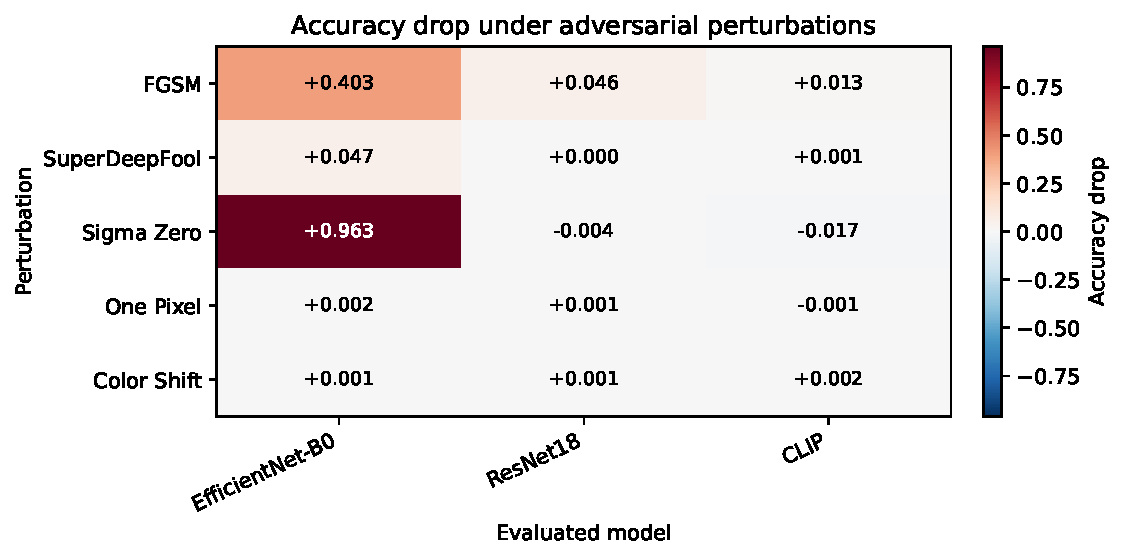
\includegraphics[width=0.88\textwidth]
{images/fig_adversarial_accuracy_drop_heatmap.pdf}
\caption{Accuracy drop of the proxy models under adversarial and
adversarial-style conditions}
\label{fig:results-adversarial-accuracy-drop-heatmap}
\end{figure}

The most severe result is observed for EfficientNet-B0 under
\gls{sigmazero}. Accuracy decreases from 0.978 to 0.015, corresponding to a
drop of 0.963. Among the 978 samples classified correctly in their clean form,
963 become incorrect, yielding an ASR of 0.9847.

The directional transitions are nearly balanced: 489 clean-correct
\texttt{weapon} samples become \texttt{non\_weapon}, while 474
clean-correct \texttt{non\_weapon} samples become \texttt{weapon}. The result
therefore represents a near-total collapse of the direct-target classifier
rather than a degradation confined to one class.

The operational consequence is twofold. The 489
\texttt{weapon}-to-\texttt{non\_weapon} transitions correspond to newly
missed firearm-oriented images, while the 474 transitions in the opposite
direction substantially increase irrelevant review workload.

\gls{fgsm} also produces severe direct-target degradation. EfficientNet-B0
accuracy decreases to 0.575, corresponding to a drop of 0.403. The attack
induces 406 errors among clean-correct samples and reaches an ASR of 0.4151.

In this case, the directional distribution is strongly asymmetric. Of the 406
induced errors, 321 are \texttt{weapon}-to-\texttt{non\_weapon}
transitions, whereas 85 occur in the opposite direction. FGSM therefore
produces a particularly relevant missed-target risk in addition to its
aggregate performance degradation.

\gls{superdeepfool} has a smaller direct-target effect. EfficientNet-B0
accuracy decreases to 0.931, producing a drop of 0.047 and an ASR of 0.0481.
All 47 induced errors occur from \texttt{non\_weapon} to \texttt{weapon};
no clean-correct \texttt{weapon} image becomes \texttt{non\_weapon} under
this condition.

This distinction is operationally important. The aggregate accuracy drop
indicates reduced correctness, but the observed direct-target failure mode
increases false-positive review workload without introducing additional missed
firearm-oriented images among the clean-correct target samples.

\gls{onepixel} produces only two direct-target induced errors on
EfficientNet-B0, one in each direction, corresponding to an ASR of 0.0020.
Its perturbed accuracy is 0.976, only 0.002 below the clean baseline. Under the
frozen parameters, this score-based condition is therefore substantially less
effective against the target architecture than Sigma-Zero, FGSM, or
SuperDeepFool.

Table~\ref{tab:results-adversarial-operational-errors} summarizes the most
relevant direct-target and transferred model-dependent conditions.

\begin{table}[H]
\centering
\scriptsize
\setlength{\tabcolsep}{3.5pt}
\renewcommand{\arraystretch}{1.15}
\caption{Operational indicators for selected model-dependent adversarial
conditions}
\label{tab:results-adversarial-operational-errors}
\begin{tabular}{@{}l l r r r r r@{}}
\toprule
\textbf{Model} &
\textbf{Attack} &
\textbf{Induced} &
\textbf{ASR} &
\textbf{Max-P shift} &
\textbf{W\(\rightarrow\)NW} &
\textbf{NW\(\rightarrow\)W} \\
\midrule

EfficientNet-B0
& \gls{sigmazero}
& 963
& 0.9847
& -0.2578
& 489
& 474 \\

EfficientNet-B0
& \gls{fgsm}
& 406
& 0.4151
& -0.1246
& 321
& 85 \\

EfficientNet-B0
& \gls{superdeepfool}
& 47
& 0.0481
& -0.3063
& 0
& 47 \\

ResNet18
& \gls{fgsm}
& 47
& 0.0488
& -0.0230
& 27
& 20 \\

\acrshort{clip}
& \gls{fgsm}
& 23
& 0.0248
& -0.0043
& 8
& 15 \\

\bottomrule
\end{tabular}

\vspace{0.4em}
\footnotesize
\textit{Note.} \textit{Induced} is the number of clean-correct samples rendered
incorrect by the perturbed condition. \textit{ASR} uses the clean-correct
denominator. \textit{Max-P shift} is the mean perturbed maximum
predicted-class probability minus the corresponding clean value.
W\(\rightarrow\)NW denotes \texttt{weapon}-to-\texttt{non\_weapon}
transitions; NW\(\rightarrow\)W denotes the opposite direction.
\end{table}

The maximum-probability shift must be interpreted independently of the
direction and number of induced errors. For example, SuperDeepFool produces the
largest negative shift among the selected EfficientNet-B0 conditions, at
\(-0.3063\), but induces substantially fewer errors than Sigma-Zero or FGSM.
Moreover, all of its induced errors occur in the false-positive direction.

The shift is computed from the maximum predicted-class probability before and
after perturbation. The maximizing class may differ between the clean and
perturbed predictions. Consequently, the value does not measure the probability
change of a fixed class and does not constitute a calibrated uncertainty
estimate.

The transfer assessment shows that perturbations optimized against
EfficientNet-B0 do not produce equivalent effects on the other proxy
architectures. The largest transferred degradation occurs under FGSM.
ResNet18 accuracy decreases from 0.964 to 0.918, corresponding to a drop of
0.046, 47 induced errors, and an ASR of 0.0488. Twenty-seven of these errors are
\texttt{weapon}-to-\texttt{non\_weapon} transitions.

For the \gls{clip}-based proxy, FGSM decreases accuracy from 0.927 to 0.914,
corresponding to a drop of 0.013. It induces 23 errors and reaches an ASR of
0.0248. Eight transitions occur from \texttt{weapon} to
\texttt{non\_weapon}, while 15 occur in the opposite direction.

Transferred Sigma-Zero artifacts do not reproduce the direct-target collapse.
ResNet18 accuracy increases by 0.004 and the \gls{clip}-based proxy accuracy
increases by 0.017. These aggregate increases nevertheless coexist with three
induced errors for ResNet18 and eight for \gls{clip}. The result again confirms
that aggregate improvement does not establish sample-level invariance.

Transferred SuperDeepFool and One Pixel artifacts produce limited effects.
SuperDeepFool induces no errors among clean-correct ResNet18 samples and three
among clean-correct \gls{clip} samples. One Pixel induces one error for
ResNet18 and none for \gls{clip} under the frozen evaluation.

Color Shift produces only marginal aggregate changes across the three
architectures. Because it is model-agnostic, its clean-correct-to-incorrect
transitions are interpreted as induced errors rather than attack or transfer
success. Its role is to provide a common adversarial-style comparison condition
rather than evidence of white-box vulnerability.

The adversarial results therefore identify a strong dependence on the
relationship between the perturbation-generation model and the evaluated
architecture. EfficientNet-B0 achieves the highest clean accuracy but undergoes
the most severe degradation when the attacks are optimized directly against
its fold-specific checkpoints. The same artifacts transfer only partially to
ResNet18 and the \gls{clip}-based proxy.

This limited transferability must not be interpreted as general robustness of
the non-target architectures. It establishes only that the frozen
EfficientNet-B0-oriented perturbations were less effective against the other
proxy models. A direct attack generated against ResNet18 or the
\gls{clip}-based proxy could produce a different result and was outside the
experimental scope.

From a forensic perspective, the findings demonstrate that high clean accuracy
does not ensure operational stability under deliberately manipulated inputs.
They also show that aggregate degradation alone is insufficient: the same
accuracy drop may represent newly missed target images, increased false-positive
workload, or a combination of both.

The output of an \gls{ai}-based classification model must therefore remain a
triage indicator rather than autonomous evidence. Its use requires systematic
human verification, traceable processing, explicit knowledge of the evaluated
threat model, and awareness that robustness conclusions are bounded to the
tested architectures, perturbations, parameters, and access assumptions.

% ─────────────────────────────────────────────────────────────────────────────
\section{Black-Box Software Results}
\label{sec:results-commercial}
% ─────────────────────────────────────────────────────────────────────────────

The implementation-specific configurations, observable output fields,
operational mappings, and normalization procedures adopted for the selected
black-box software systems are documented in
Section~\ref{sec:implementation-forensic-tools}. The present section reports
the resulting normalized behavior without making assumptions about inaccessible
internal architectures, training data, thresholds, or confidence-calibration
procedures.

The analysis comprises four software families and six normalized operational
configurations:

\begin{itemize}
\item \gls{magnetaxiomtool}/\gls{magnetai};
\item \gls{griffeye}/\gls{t3kcore};
\item \gls{excirefoto2025} under the \texttt{D20}, \texttt{D50}, and
\texttt{D80} semantic-distance settings;
\item \gls{cellebriteinseyets}.
\end{itemize}

Each configuration produced one normalized decision for every item in the
11\,500-file forensic evaluation bundle. The complete black-box population
therefore contains:

\begin{equation}
6\ \text{normalized configurations}
\times
11\,500\ \text{bundle items}
=
69\,000\ \text{matched decisions}.
\end{equation}

No bundle item remained without a matched normalized decision, and the
canonical public population contains no \texttt{unknown} outputs. Non-bundle
records present in some controlled raw exports were excluded during
normalization, as described in
Section~\ref{subsec:implementation-normalization}.

The 11\,500 matched decisions associated with each configuration comprise two
analytically distinct populations:

\begin{itemize}
\item 11\,000 binary items with a reference operational assignment of
\texttt{weapon} or \texttt{non\_weapon};

\item 500 \gls{ood} inputs, analyzed separately through their observable
weapon assignment rate.
\end{itemize}

Accuracy, balanced accuracy, precision, recall, \gls{fnr}, and \gls{fpr} are
computed only on the 11\,000 interpretable binary items. The \gls{ood} inputs
are excluded from those metrics because they have no binary reference
assignment.

The binary aggregate is itself bundle-weighted rather than
condition-balanced. It contains 1\,000 clean inputs and 10\,000 perturbed
artifacts:

\begin{equation}
N_{\mathrm{binary}}
=
1\,000\ \text{clean inputs}
+
5\,000\ \text{adversarial artifacts}
+
5\,000\ \text{anti-forensic artifacts}
=
11\,000.
\end{equation}

Consequently, the bundle-level metrics are influenced primarily by behavior on
the perturbed population. They must not be interpreted as the arithmetic mean
of clean, adversarial, and anti-forensic performance, nor as estimates of the
frequency with which these conditions would occur in an operational case.

The four model-dependent adversarial conditions were generated against
fold-specific EfficientNet-B0 checkpoints. Their evaluation through the
selected black-box software systems therefore constitutes an empirical transfer
assessment. It does not constitute a white-box attack against any commercial
system. \gls{colorshift} instead provides a deterministic model-agnostic
comparison condition.

Table~\ref{tab:results-commercial-overview} summarizes the normalized results
for the six configurations.

\begin{table}[H]
\centering
\scriptsize
\renewcommand{\arraystretch}{1.15}
\setlength{\tabcolsep}{2.6pt}
\caption{Bundle-weighted summary of the selected black-box software
configurations}
\label{tab:results-commercial-overview}
\resizebox{\textwidth}{!}{%
\begin{tabular}{@{}l r r r r r r r r@{}}
\toprule
\textbf{Configuration} &
\textbf{Matched} &
\textbf{Clean \acrshort{fnr}} &
\textbf{Bundle Acc.} &
\textbf{Bundle Bal.} &
\textbf{Bundle R\textsubscript{w}} &
\textbf{Bundle \acrshort{fnr}} &
\textbf{Bundle \acrshort{fpr}} &
\textbf{\acrshort{ood} W-rate} \\
\midrule

\gls{magnetaxiomtool}/\gls{magnetai}
& 11\,500
& 0.070
& 0.933
& 0.933
& 0.901
& 0.099
& 0.035
& 0.360 \\

\gls{griffeye}/\gls{t3kcore}
& 11\,500
& 0.036
& 0.972
& 0.972
& 0.951
& 0.049
& 0.007
& 0.260 \\

\gls{excirefoto2025} \texttt{D20}
& 11\,500
& 0.120
& 0.911
& 0.911
& 0.857
& 0.143
& 0.036
& 0.238 \\

\gls{excirefoto2025} \texttt{D50}
& 11\,500
& 0.042
& 0.925
& 0.925
& 0.949
& 0.051
& 0.099
& 0.340 \\

\gls{excirefoto2025} \texttt{D80}
& 11\,500
& 0.014
& 0.887
& 0.887
& 0.981
& 0.019
& 0.207
& 0.522 \\

\gls{cellebriteinseyets}
& 11\,500
& 0.032
& 0.958
& 0.958
& 0.958
& 0.042
& 0.042
& 0.292 \\

\bottomrule
\end{tabular}%
}

\vspace{0.4em}
\footnotesize
\textit{Note.} \textit{Matched} indicates the complete 11\,500-item bundle
population associated with each normalized configuration. Clean
\acrshort{fnr} is computed on the 1\,000 unperturbed binary inputs. Bundle
accuracy, balanced accuracy, weapon recall, \acrshort{fnr}, and \acrshort{fpr}
are computed on the 11\,000-item binary population, comprising clean,
adversarial, and anti-forensic samples and excluding \gls{ood} inputs.
\textit{\acrshort{ood} W-rate} indicates the proportion of the 500
\gls{ood} inputs assigned to \texttt{weapon}. The bundle-level values reflect
the frozen experimental composition and do not constitute general validation
or an absolute ranking of the selected software systems.
\end{table}

Figure~\ref{fig:results-forensic-tools-global-comparison} visualizes the same
bundle-weighted metrics.

\begin{figure}[H]
\centering
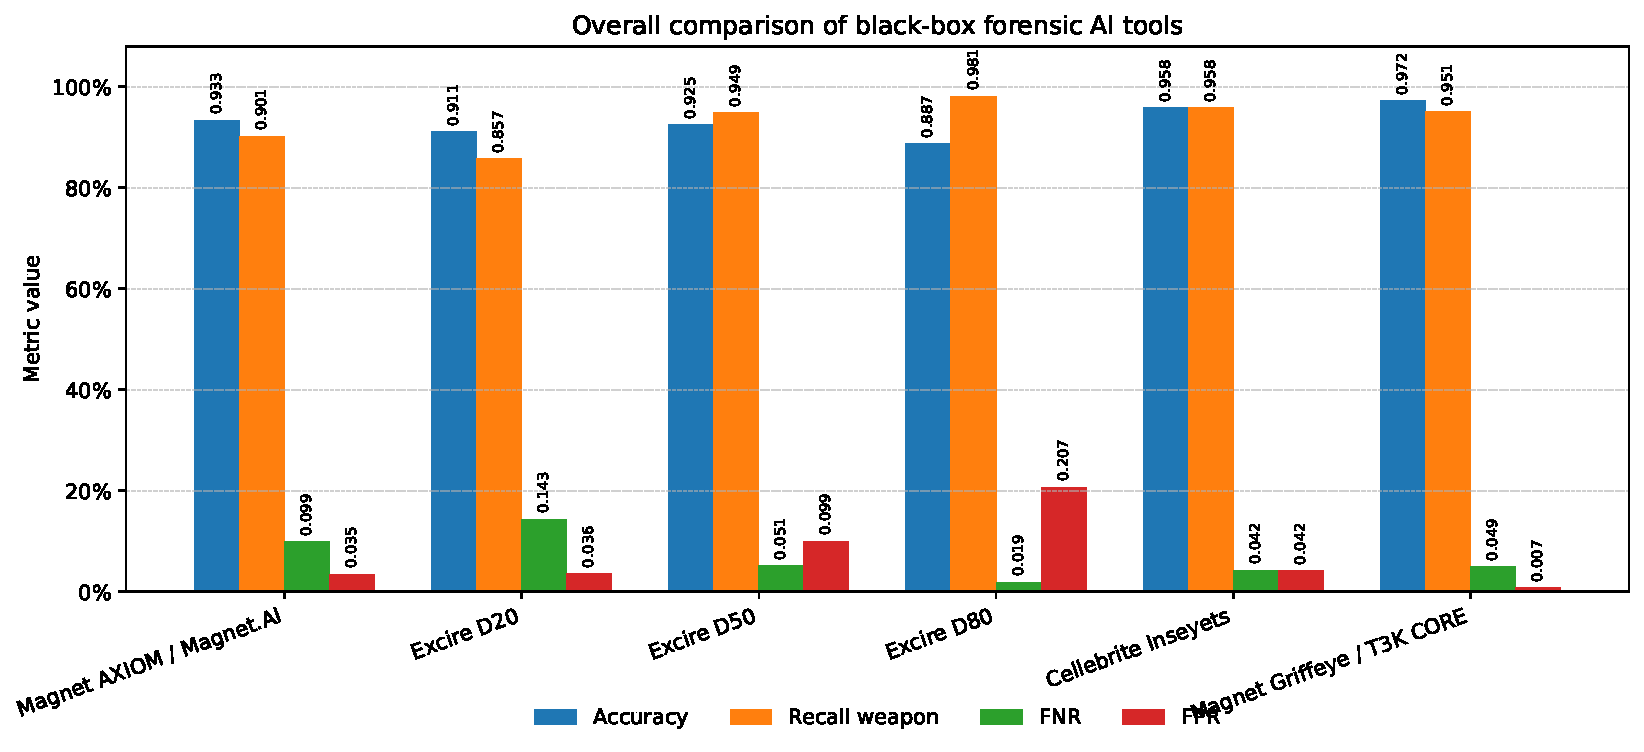
\includegraphics[width=\textwidth]
{images/fig_forensic_tools_global_metrics_comparison.pdf}
\caption{Bundle-weighted normalized metrics of the selected black-box software
configurations}
\label{fig:results-forensic-tools-global-comparison}
\end{figure}

The aggregate comparison identifies distinct operational profiles, but it must
not be interpreted as a direct ranking of intrinsic system quality. The
evaluated software systems differ in intended use, internal taxonomy,
observable output semantics, configuration, and decision mechanism.
Furthermore, the binary bundle contains repeated manipulated versions derived
from the same 1\,000 source images rather than 11\,000 independent real-world
cases.

Within the frozen protocol, \gls{griffeye}/\gls{t3kcore} exhibits the highest
bundle-level accuracy, at 0.972, and the lowest \gls{fpr}, at 0.007. Its
weapon recall is 0.951, corresponding to a bundle \gls{fnr} of 0.049.

\gls{cellebriteinseyets} presents a comparatively balanced profile. Its bundle
accuracy is 0.958, weapon recall is 0.958, \gls{fnr} is 0.042, and
\gls{fpr} is 0.042.

\gls{magnetaxiomtool}/\gls{magnetai} achieves a bundle accuracy of 0.933 and
an \gls{fpr} of 0.035. Its weapon recall is lower, at 0.901, corresponding to
a bundle \gls{fnr} of 0.099. Its clean \gls{fnr}, at 0.070, is lower than the
bundle-weighted value, indicating a larger missed-target proportion across the
combined perturbed population.

The three \gls{excirefoto2025} configurations expose the clearest
configuration-dependent tradeoff. At \texttt{D20}, the system produces a
relatively low \gls{fpr} of 0.036 and the lowest \gls{ood} weapon assignment
rate, at 0.238, but its weapon recall is 0.857 and its \gls{fnr} is 0.143.

At \texttt{D50}, weapon recall increases to 0.949 and the \gls{fnr} decreases
to 0.051. This improvement is accompanied by an \gls{fpr} of 0.099 and an
\gls{ood} weapon assignment rate of 0.340.

At \texttt{D80}, weapon recall reaches 0.981 and the \gls{fnr} decreases to
0.019, the lowest among the six configurations. However, the \gls{fpr}
increases to 0.207, and the \gls{ood} weapon assignment rate reaches 0.522.
The broader retrieval setting therefore minimizes missed firearm-oriented
content at the cost of a substantially larger false-positive review burden.

The Excire results demonstrate why a configuration with lower \gls{fnr} is not
automatically preferable in every operational context. Increasing retrieval
coverage can reduce missed detections while simultaneously increasing the
quantity of \texttt{non\_weapon} and \gls{ood} material routed to the
firearm-oriented review category.

Figure~\ref{fig:results-forensic-tools-ood-weapon-flag-rate} reports the
observable weapon assignment rate on the separate \gls{ood} branch.

\begin{figure}[H]
\centering
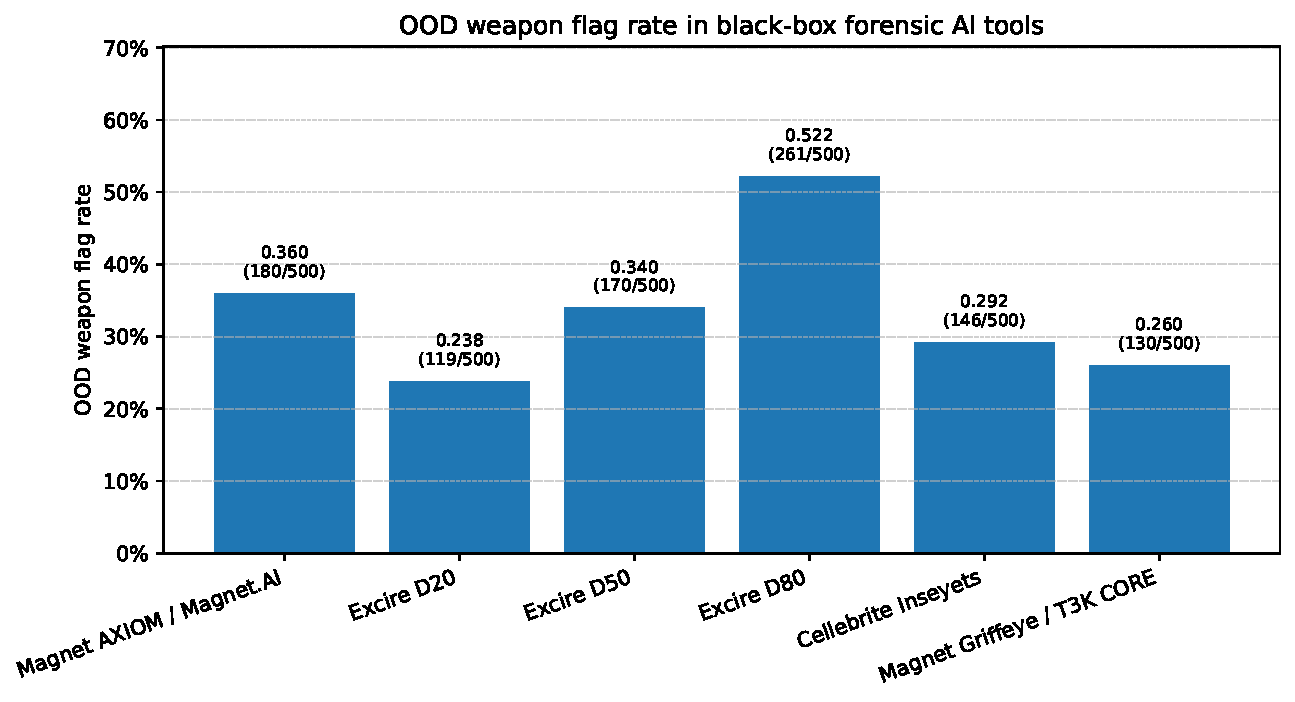
\includegraphics[width=0.90\textwidth]
{images/fig_forensic_tools_ood_weapon_flag_rate.pdf}
\caption{Weapon assignment rate of the selected black-box software
configurations on \gls{ood} inputs}
\label{fig:results-forensic-tools-ood-weapon-flag-rate}
\end{figure}

Every configuration assigns a non-zero proportion of the 500 \gls{ood} inputs
to the operational \texttt{weapon} class. These assignments are not false
positives in the supervised binary sense because the \gls{ood} inputs have no
\texttt{weapon} or \texttt{non\_weapon} reference assignment.

Nevertheless, the assignments remain operationally relevant. They may increase
the amount of unrelated material prioritized for analyst review and may alter
the ordering of content outside the nominal binary task. The lowest observed
rate is 0.238 for Excire \texttt{D20}, whereas the highest is 0.522 for
Excire \texttt{D80}. The other configurations fall between these values:
0.260 for Griffeye/T3K CORE, 0.292 for Cellebrite Inseyets, 0.340 for Excire
\texttt{D50}, and 0.360 for Magnet AXIOM/Magnet.AI.

The overview therefore identifies no single configuration that simultaneously
minimizes false negatives, false positives, and \gls{ood} weapon assignments.
The selected systems expose different tradeoffs between missed-target risk and
human-review workload. Their operational suitability cannot be inferred from a
single aggregate metric and must be evaluated in relation to the intended
forensic workflow, the consequences of each error direction, and the continued
availability of human verification.


\subsection{\texorpdfstring{\gls{magnetaxiomtool}/\gls{magnetai}}{Magnet AXIOM/Magnet.AI} Results}
\label{subsec:results-magnet}
% ─────────────────────────────────────────────────────────────────────────────

The observable output mapping and normalization procedure adopted for
\gls{magnetaxiomtool}/\gls{magnetai} are documented in
Section~\ref{subsec:implementation-magnet}. The present subsection reports the
resulting normalized behavior without making assumptions about the inaccessible
internal classifier, decision threshold, or training data.

All 11\,500 bundle files were associated with one normalized output. Binary
metrics are computed on the 11\,000 items whose reference operational
assignment is \texttt{weapon} or \texttt{non\_weapon}. The separate 500-image
\gls{ood} branch is analyzed through the proportion of inputs receiving a
weapon-oriented assignment.

Under the frozen mapping, the exported \texttt{Possible weapons} tag is treated
as the primary positive observable output. Absence of the tag is mapped to
\texttt{non\_weapon}, while the defensive normalization rules described in
Section~\ref{subsec:implementation-magnet} preserve any unsupported nonempty
state as \texttt{unknown}. No such unknown state occurs in the canonical
11\,500-item result population.

Table~\ref{tab:results-magnet-global-metrics} reports the bundle-weighted
binary metrics.

\begin{table}[H]
\centering
\caption{Bundle-weighted performance of \gls{magnetai} on the binary
\texttt{weapon}/\texttt{non\_weapon} task}
\label{tab:results-magnet-global-metrics}
\small
\begin{tabular}{@{}l r@{}}
\toprule
\textbf{Metric} &
\textbf{Value} \\
\midrule

Accuracy
& 0.933 \\

Balanced accuracy
& 0.933 \\

Precision \texttt{weapon}
& 0.963 \\

Recall \texttt{weapon}
& 0.901 \\

F1-score \texttt{weapon}
& 0.931 \\

False negative rate
& 0.099 \\

False positive rate
& 0.035 \\

True positives
& 4\,958 \\

True negatives
& 5\,309 \\

False positives
& 191 \\

False negatives
& 542 \\

\bottomrule
\end{tabular}

\vspace{0.4em}
\footnotesize
\textit{Note.} The metrics are computed on the 11\,000-item binary bundle,
comprising 1\,000 clean inputs and 10\,000 perturbed artifacts. The values are
therefore bundle-weighted and do not represent an arithmetic mean across
experimental conditions.
\end{table}

Within the frozen binary bundle, \gls{magnetai} achieves an accuracy and
balanced accuracy of 0.933. Precision for the \texttt{weapon} class is 0.963,
indicating that most files assigned the positive operational state are
reference \texttt{weapon} samples.

Weapon recall is lower, at 0.901, corresponding to an \gls{fnr} of 0.099.
Across the 5\,500 reference \texttt{weapon} items in the binary bundle, 542 do
not receive the positive observable tag. The \gls{fpr} is 0.035, corresponding
to 191 \texttt{non\_weapon} items assigned to the operational
\texttt{weapon} class.

These aggregate values must be interpreted in relation to the composition of
the bundle. Perturbed artifacts outnumber clean inputs by ten to one.
Consequently, the overall metrics primarily describe behavior across the
combined perturbed population rather than nominal clean-condition performance.

Table~\ref{tab:results-magnet-condition-metrics} separates the clean,
perturbed, adversarial-family, anti-forensic-family, and \gls{ood} results.

\begin{table}[H]
\centering
\caption{Behavior of \gls{magnetai} by experimental condition}
\label{tab:results-magnet-condition-metrics}
\small
\begin{tabularx}{\textwidth}{@{}l r r r r X@{}}
\toprule
\textbf{Condition} &
\textbf{Accuracy} &
\textbf{Recall weapon} &
\textbf{\gls{fnr}} &
\textbf{\gls{fpr}} &
\textbf{Operational interpretation} \\
\midrule

Clean
&
0.950
&
0.930
&
0.070
&
0.030
&
Baseline behavior on 1\,000 unperturbed binary inputs. \\

Perturbed
&
0.932
&
0.899
&
0.101
&
0.035
&
Aggregate behavior on 10\,000 artifacts: 5\,000 adversarial or
adversarial-style variants and 5\,000 anti-forensic variants. \\

Adversarial family
&
0.923
&
0.884
&
0.116
&
0.038
&
Aggregate transfer behavior across four EfficientNet-B0-oriented attacks and
the model-agnostic Color Shift condition. \\

Anti-forensic family
&
0.940
&
0.913
&
0.087
&
0.032
&
Aggregate behavior across the five model-agnostic anti-forensic
transformations. \\

\gls{ood}
&
--
&
--
&
--
&
--
&
A total of 180 of the 500 \gls{ood} inputs receive the
\texttt{Possible weapons} tag, corresponding to a weapon assignment rate of
0.360. Binary correctness metrics are not applicable. \\

\bottomrule
\end{tabularx}
\end{table}

The clean baseline yields an accuracy of 0.950, a weapon recall of 0.930, an
\gls{fnr} of 0.070, and an \gls{fpr} of 0.030. This corresponds to 35 missed
\texttt{weapon} images and 15 false-positive assignments among the 1\,000
unperturbed inputs.

Across the complete perturbed population, accuracy decreases to 0.932 and
weapon recall decreases to 0.899. The \gls{fnr} consequently increases to
0.101, while the \gls{fpr} increases more moderately to 0.035. The principal
aggregate change therefore concerns a greater proportion of missed
firearm-oriented inputs.

The adversarial-family population produces a stronger effect than the
anti-forensic population under the frozen protocol. Its accuracy is 0.923,
weapon recall is 0.884, and \gls{fnr} is 0.116. The anti-forensic population
retains an accuracy of 0.940, weapon recall of 0.913, and \gls{fnr} of 0.087.

This comparison does not establish that Magnet.AI was directly attacked in a
white-box setting. The four model-dependent adversarial artifacts were
generated against fold-specific EfficientNet-B0 checkpoints and were only
subsequently processed by Magnet.AI. Their effects therefore measure empirical
transfer behavior. Color Shift and the anti-forensic transformations are
model-agnostic conditions.

The separate \gls{ood} result is also operationally relevant. Of the 500
inputs outside the binary reference task, 180 receive the
\texttt{Possible weapons} tag. The resulting rate of 0.360 is not a supervised
false-positive rate because these inputs have no \texttt{weapon} or
\texttt{non\_weapon} reference assignment.

Nevertheless, these assignments may increase the quantity of unrelated
material prioritized for analyst review. The result describes the observable
closed-set behavior of the frozen configuration and does not establish the
investigative relevance of the individual \gls{ood} images.

Unlike the proxy models, \gls{magnetai} does not expose a homogeneous numerical
probability or uncertainty value for the adopted image-level output. The
analysis is therefore limited to the observable categorical tag and cannot
include probability-distribution, calibration, or maximum-probability
comparisons with the proxy architectures.

Table~\ref{tab:results-magnet-attack-metrics} reports the condition-level
behavior for all ten perturbed populations.

\begin{table}[H]
\centering
\caption{Performance of \gls{magnetai} under adversarial, adversarial-style,
and anti-forensic conditions}
\label{tab:results-magnet-attack-metrics}
\scriptsize
\renewcommand{\arraystretch}{1.12}
\setlength{\tabcolsep}{4pt}
\begin{tabular}{@{}l l r r r r r r@{}}
\toprule
\textbf{Family} &
\textbf{Condition} &
\textbf{Accuracy} &
\textbf{Recall} &
\textbf{\gls{fnr}} &
\textbf{\gls{fpr}} &
\textbf{\acrshort{fn}} &
\textbf{\acrshort{fp}} \\
\midrule

Adversarial-style
&
\gls{colorshift}
&
0.951
&
0.934
&
0.066
&
0.032
&
33
&
16 \\

Adversarial transfer
&
\gls{fgsm}
&
0.867
&
0.808
&
0.192
&
0.074
&
96
&
37 \\

Adversarial transfer
&
\gls{onepixel}
&
0.950
&
0.930
&
0.070
&
0.030
&
35
&
15 \\

Adversarial transfer
&
\gls{sigmazero}
&
0.916
&
0.856
&
0.144
&
0.024
&
72
&
12 \\

Adversarial transfer
&
\gls{superdeepfool}
&
0.932
&
0.894
&
0.106
&
0.030
&
53
&
15 \\

\midrule

Anti-forensic
&
\gls{contraststretching}
&
0.951
&
0.930
&
0.070
&
0.028
&
35
&
14 \\

Anti-forensic
&
\gls{gaussianblur}
&
0.927
&
0.880
&
0.120
&
0.026
&
60
&
13 \\

Anti-forensic
&
\gls{histogrammodification}
&
0.936
&
0.920
&
0.080
&
0.048
&
40
&
24 \\

Anti-forensic
&
\gls{jpegrecompression}
&
0.944
&
0.928
&
0.072
&
0.040
&
36
&
20 \\

Anti-forensic
&
\gls{resampleresize}
&
0.943
&
0.906
&
0.094
&
0.020
&
47
&
10 \\

\bottomrule
\end{tabular}
\end{table}

Among the transferred model-dependent adversarial conditions, \gls{fgsm}
produces the most substantial degradation. Accuracy decreases to 0.867 and
weapon recall to 0.808, while the \gls{fnr} increases to 0.192. This
corresponds to 96 missed \texttt{weapon} items and 37 false-positive
assignments in the 1\,000-item FGSM population.

Transferred Sigma-Zero artifacts produce the second-highest missed-target
burden. Accuracy is 0.916, weapon recall is 0.856, and the \gls{fnr} is 0.144,
corresponding to 72 false negatives. SuperDeepFool produces an \gls{fnr} of
0.106 and 53 false negatives.

One Pixel produces the same aggregate confusion-matrix values as the clean
baseline: accuracy 0.950, \gls{fnr} 0.070, and \gls{fpr} 0.030. This result is
specific to the frozen transferred artifacts and does not establish general
invariance to score-based attacks generated directly against Magnet.AI.

The model-agnostic Color Shift condition produces an accuracy of 0.951 and an
\gls{fnr} of 0.066, values close to the clean baseline. Because it was not
optimized against a model, its effect is interpreted as condition-specific
behavior rather than adversarial transfer success.

Among the anti-forensic transformations, Gaussian Blur produces the largest
missed-target effect. Weapon recall decreases to 0.880 and the \gls{fnr}
increases to 0.120, corresponding to 60 false negatives. Histogram
Modification produces a lower \gls{fnr}, at 0.080, but the highest
anti-forensic \gls{fpr}, at 0.048, corresponding to 24 false positives.

The remaining transformations produce smaller changes but do not preserve the
same operational profile. JPEG Recompression yields 36 false negatives and 20
false positives, while Resample Resize yields 47 false negatives and 10 false
positives. Contrast Stretching remains close to the clean baseline.

The results therefore identify failure modes that are not captured by overall
accuracy alone. FGSM transfer and Gaussian Blur primarily increase the
proportion of firearm-oriented inputs not receiving the positive tag, whereas
Histogram Modification produces a comparatively greater increase in
false-positive review workload.

These findings describe the normalized observable behavior of the frozen
\gls{magnetaxiomtool}/\gls{magnetai} configuration. They do not reveal the
internal model architecture, establish a general vulnerability of the
commercial platform, or support extrapolation to other software versions,
categories, thresholds, or media-analysis configurations.

The \texttt{Possible weapons} tag must therefore remain a triage aid rather
than a self-sufficient evidentiary conclusion. Its operational use requires
human verification, awareness of the false-negative risk under both clean and
perturbed conditions, and traceable documentation of the software version,
configuration, imported population, and output-normalization rule.



% ─────────────────────────────────────────────────────────────────────────────
\subsection{\texorpdfstring{\gls{griffeye}/\gls{t3kcore}}{Magnet Griffeye/T3K CORE} Results}
\label{subsec:results-griffeye}
% ─────────────────────────────────────────────────────────────────────────────

The observable bookmark mapping and normalization procedure adopted for
\gls{griffeye}/\gls{t3kcore} are documented in
Section~\ref{subsec:implementation-griffeye}. The present subsection reports
the resulting normalized behavior without making assumptions about the
inaccessible internal classification architecture, thresholds, preprocessing,
or bookmark-generation criteria.

All 11\,500 bundle files were associated with a normalized decision. Binary
metrics are computed on the 11\,000 items whose reference operational
assignment is \texttt{weapon} or \texttt{non\_weapon}, whereas the 500
\gls{ood} inputs are analyzed separately through their weapon assignment rate.

Under the frozen operational mapping, only the
\texttt{CORE/Violence/Firearm} bookmark is treated as a positive
\texttt{weapon} output. Other bookmarks related to weapons, violence,
military equipment, or adjacent semantic categories are preserved in the
controlled raw output but are not included as primary positives.

This mapping is deliberately conservative. Consequently, the observed false
positive rate must be interpreted jointly with the selected bookmark rule. A
more permissive mapping incorporating secondary weapon-related bookmarks would
define a different operational task and could alter both target recall and
false-positive review workload. That alternative was not evaluated in the
frozen protocol.

Table~\ref{tab:results-griffeye-global-metrics} reports the bundle-weighted
binary results.

\begin{table}[H]
\centering
\caption{Bundle-weighted performance of
\gls{griffeye}/\gls{t3kcore} on the binary
\texttt{weapon}/\texttt{non\_weapon} task}
\label{tab:results-griffeye-global-metrics}
\small
\begin{tabular}{@{}l r@{}}
\toprule
\textbf{Metric} &
\textbf{Value} \\
\midrule

Accuracy
& 0.972 \\

Balanced accuracy
& 0.972 \\

Precision \texttt{weapon}
& 0.992 \\

Recall \texttt{weapon}
& 0.951 \\

F1-score \texttt{weapon}
& 0.971 \\

False negative rate
& 0.049 \\

False positive rate
& 0.007 \\

True positives
& 5\,229 \\

True negatives
& 5\,460 \\

False positives
& 40 \\

False negatives
& 271 \\

\bottomrule
\end{tabular}

\vspace{0.4em}
\footnotesize
\textit{Note.} The metrics are computed on the 11\,000-item binary bundle,
comprising 1\,000 clean inputs and 10\,000 perturbed artifacts. The 500
\gls{ood} inputs are excluded from binary correctness metrics. The low
\acrshort{fpr} must also be interpreted in relation to the conservative
positive mapping based exclusively on the
\texttt{CORE/Violence/Firearm} bookmark.
\end{table}

Within the frozen binary bundle, \gls{griffeye}/\gls{t3kcore} achieves an
accuracy and balanced accuracy of 0.972. Precision for the
\texttt{weapon} class is 0.992, corresponding to only 40 false-positive
assignments among the 5\,500 reference \texttt{non\_weapon} items.

Weapon recall is 0.951, corresponding to an \gls{fnr} of 0.049. A total of
271 reference \texttt{weapon} items are therefore not associated with the
primary firearm bookmark.

The result represents the highest bundle-level accuracy and the lowest
bundle-level \gls{fpr} among the six normalized configurations under the
frozen protocol. It must not be interpreted as evidence of intrinsically
superior system quality because it is conditional on the evaluated software
version, the selected category, the imported population, and the conservative
normalization rule.

Table~\ref{tab:results-griffeye-condition-metrics} separates clean,
perturbed, adversarial-family, anti-forensic-family, and \gls{ood} behavior.

\begin{table}[H]
\centering
\caption{Behavior of \gls{griffeye}/\gls{t3kcore} by experimental condition}
\label{tab:results-griffeye-condition-metrics}
\small
\begin{tabularx}{\textwidth}{@{}l r r r r X@{}}
\toprule
\textbf{Condition} &
\textbf{Accuracy} &
\textbf{Recall weapon} &
\textbf{\gls{fnr}} &
\textbf{\gls{fpr}} &
\textbf{Operational interpretation} \\
\midrule

Clean
&
0.978
&
0.964
&
0.036
&
0.008
&
Baseline behavior on 1\,000 unperturbed binary inputs. \\

Perturbed
&
0.971
&
0.949
&
0.051
&
0.007
&
Aggregate behavior on 10\,000 artifacts: 5\,000 adversarial or
adversarial-style variants and 5\,000 anti-forensic variants. \\

Adversarial family
&
0.969
&
0.945
&
0.055
&
0.008
&
Aggregate transfer behavior across four EfficientNet-B0-oriented attacks and
the model-agnostic Color Shift condition. \\

Anti-forensic family
&
0.974
&
0.954
&
0.046
&
0.006
&
Aggregate behavior across the five model-agnostic anti-forensic
transformations. \\

\gls{ood}
&
--
&
--
&
--
&
--
&
A total of 130 of the 500 \gls{ood} inputs are assigned to the operational
\texttt{weapon} state, corresponding to a weapon assignment rate of 0.260.
Binary correctness metrics are not applicable. \\

\bottomrule
\end{tabularx}
\end{table}

The clean baseline produces an accuracy of 0.978, weapon recall of 0.964,
\gls{fnr} of 0.036, and \gls{fpr} of 0.008. This corresponds to 18 missed
\texttt{weapon} inputs and four false-positive assignments among the 1\,000
clean images.

Across the 10\,000 perturbed artifacts, accuracy decreases to 0.971 and weapon
recall decreases to 0.949. The \gls{fnr} increases to 0.051, whereas the
\gls{fpr} remains slightly lower than the clean value, at 0.007. The primary
aggregate change therefore concerns a moderate increase in missed
firearm-oriented inputs rather than increased false-positive workload.

The adversarial-family population produces an accuracy of 0.969, weapon recall
of 0.945, and \gls{fnr} of 0.055. The anti-forensic population exhibits an
accuracy of 0.974, weapon recall of 0.954, and \gls{fnr} of 0.046.

The difference between the two families is limited but directionally
consistent: under the frozen protocol, the transferred adversarial artifacts
produce a somewhat larger missed-target burden than the model-agnostic
anti-forensic transformations.

This comparison does not constitute a white-box attack against
\gls{griffeye}/\gls{t3kcore}. The four model-dependent adversarial populations
were generated against fold-specific EfficientNet-B0 checkpoints. Their
evaluation through Griffeye/T3K CORE measures only empirical transfer behavior.

On the separate \gls{ood} branch, 130 of the 500 inputs receive the primary
firearm-oriented operational assignment, yielding a weapon assignment rate of
0.260. These outputs are not false positives in the supervised binary sense
because the \gls{ood} inputs have no \texttt{weapon} or
\texttt{non\_weapon} reference assignment.

Nevertheless, the result remains operationally relevant. Even a configuration
with a low binary \gls{fpr} may route material outside the nominal task toward
the firearm-oriented review category, thereby increasing analyst workload or
altering prioritization.

Table~\ref{tab:results-griffeye-attack-metrics} reports the ten individual
perturbed conditions.

\begin{table}[H]
\centering
\scriptsize
\renewcommand{\arraystretch}{1.12}
\setlength{\tabcolsep}{4pt}
\caption{Performance of \gls{griffeye}/\gls{t3kcore} under adversarial,
adversarial-style, and anti-forensic conditions}
\label{tab:results-griffeye-attack-metrics}
\begin{tabular}{@{}l l r r r r r r@{}}
\toprule
\textbf{Family} &
\textbf{Condition} &
\textbf{Accuracy} &
\textbf{Recall} &
\textbf{\gls{fnr}} &
\textbf{\gls{fpr}} &
\textbf{\acrshort{fn}} &
\textbf{\acrshort{fp}} \\
\midrule

Adversarial-style
&
\gls{colorshift}
&
0.977
&
0.960
&
0.040
&
0.006
&
20
&
3 \\

Adversarial transfer
&
\gls{fgsm}
&
0.960
&
0.928
&
0.072
&
0.008
&
36
&
4 \\

Adversarial transfer
&
\gls{onepixel}
&
0.978
&
0.964
&
0.036
&
0.008
&
18
&
4 \\

Adversarial transfer
&
\gls{sigmazero}
&
0.959
&
0.926
&
0.074
&
0.008
&
37
&
4 \\

Adversarial transfer
&
\gls{superdeepfool}
&
0.969
&
0.948
&
0.052
&
0.010
&
26
&
5 \\

\midrule

Anti-forensic
&
\gls{contraststretching}
&
0.977
&
0.964
&
0.036
&
0.010
&
18
&
5 \\

Anti-forensic
&
\gls{gaussianblur}
&
0.972
&
0.948
&
0.052
&
0.004
&
26
&
2 \\

Anti-forensic
&
\gls{histogrammodification}
&
0.963
&
0.932
&
0.068
&
0.006
&
34
&
3 \\

Anti-forensic
&
\gls{jpegrecompression}
&
0.976
&
0.960
&
0.040
&
0.008
&
20
&
4 \\

Anti-forensic
&
\gls{resampleresize}
&
0.980
&
0.964
&
0.036
&
0.004
&
18
&
2 \\

\bottomrule
\end{tabular}
\end{table}

Among the transferred model-dependent conditions, Sigma-Zero produces the
largest missed-target burden. Accuracy decreases to 0.959, weapon recall to
0.926, and the \gls{fnr} increases to 0.074, corresponding to 37 false
negatives and four false positives.

FGSM produces a closely related profile, with an accuracy of 0.960, weapon
recall of 0.928, and \gls{fnr} of 0.072. The population contains 36 false
negatives and four false positives.

The transferred Sigma-Zero artifacts therefore produce measurable degradation
but do not reproduce the near-total collapse observed for their direct
EfficientNet-B0 target. This difference is evidence of limited transfer under
the evaluated conditions, not proof of general robustness against attacks
generated directly against Griffeye/T3K CORE.

SuperDeepFool produces an accuracy of 0.969 and an \gls{fnr} of 0.052.
One Pixel preserves the same aggregate confusion-matrix values as the clean
baseline, with 18 false negatives and four false positives. This result is
specific to the frozen transferred population.

The model-agnostic Color Shift condition remains close to the clean baseline,
with an accuracy of 0.977, \gls{fnr} of 0.040, and \gls{fpr} of 0.006. Its
effect is interpreted as condition-specific behavior rather than adversarial
transfer success.

Among the anti-forensic transformations, Histogram Modification produces the
largest missed-target effect. Accuracy decreases to 0.963, weapon recall to
0.932, and the \gls{fnr} increases to 0.068, corresponding to 34 false
negatives.

Gaussian Blur produces 26 false negatives but only two false positives.
JPEG Recompression produces 20 false negatives and four false positives.
Contrast Stretching produces the highest anti-forensic \gls{fpr}, at 0.010,
although this corresponds to only five false-positive assignments.

Resample Resize produces the highest condition-level accuracy, at 0.980, while
retaining 18 false negatives and two false positives. The slightly higher
accuracy than the clean baseline does not establish sample-level invariance:
aggregate improvements may coexist with changed individual decisions.

Overall, the frozen Griffeye/T3K CORE configuration combines high
firearm-oriented recall with a particularly low false-positive rate. The
profile is operationally selective, but its interpretation is inseparable from
the conservative choice to count only
\texttt{CORE/Violence/Firearm} as a primary positive.

The results do not reveal whether the observed behavior derives from the
internal model architecture, proprietary preprocessing, semantic thresholds,
bookmark taxonomy, or other inaccessible implementation factors. They also do
not support extrapolation to alternative bookmark mappings, software versions,
categories, or operational configurations.

The automatic firearm bookmark must therefore remain a triage signal rather
than an autonomous evidentiary conclusion. Its use requires human verification
and traceable documentation of the software version, enabled processing
modules, imported population, and normalization rule.

% ─────────────────────────────────────────────────────────────────────────────
\subsection{\texorpdfstring{\gls{excirefoto2025}}{Excire Foto 2025} Results and Sensitivity Analysis}
\label{subsec:results-excire}
% ─────────────────────────────────────────────────────────────────────────────

The semantic-retrieval mapping and the three frozen
\texttt{Distance limit} settings are documented in
Section~\ref{subsec:implementation-excire}. The present subsection examines how
the normalized operational behavior changes across the \texttt{D20},
\texttt{D50}, and \texttt{D80} configurations.

The software was evaluated using the same eight firearm-oriented semantic
queries under each distance setting. An image was mapped to the operational
\texttt{weapon} state when it appeared in the result set of at least one of
the eight queries. Consequently, the reported decisions represent the union of
the observable prompt-hit sets rather than an internal binary classifier output.

The three configurations differ only in the frozen semantic-distance setting:

\begin{itemize}
\item \texttt{D20} represents the most restrictive evaluated retrieval
configuration;

\item \texttt{D50} represents the intermediate configuration;

\item \texttt{D80} represents the most permissive evaluated configuration.
\end{itemize}

The terms restrictive, intermediate, and permissive describe only the relative
behavior of the three evaluated settings. They do not reveal the internal
scoring function, semantic embedding space, or decision mechanism used by the
software.

Table~\ref{tab:results-excire-sensitivity} reports clean binary performance and
\gls{ood} weapon assignment behavior for the three configurations.

\begin{table}[H]
\centering
\scriptsize
\renewcommand{\arraystretch}{1.15}
\setlength{\tabcolsep}{4pt}
\caption{Sensitivity of \gls{excirefoto2025} to the
\texttt{Distance limit} setting}
\label{tab:results-excire-sensitivity}
\begin{tabularx}{0.96\textwidth}{@{}l r r r r r X@{}}
\toprule
\textbf{Setting} &
\textbf{Clean Acc.} &
\textbf{Clean R\textsubscript{w}} &
\textbf{Clean \gls{fnr}} &
\textbf{Clean \gls{fpr}} &
\textbf{\acrshort{ood} W-rate} &
\textbf{Operational profile} \\
\midrule

\texttt{D20}
&
0.927
&
0.880
&
0.120
&
0.026
&
0.238
&
Restrictive profile with the lowest clean false-positive rate and the lowest
\gls{ood} weapon assignment rate, but the highest clean missed-target rate. \\

\texttt{D50}
&
0.944
&
0.958
&
0.042
&
0.070
&
0.340
&
Intermediate profile balancing target recall, false-positive workload, and
\gls{ood} weapon assignments. \\

\texttt{D80}
&
0.915
&
0.986
&
0.014
&
0.156
&
0.522
&
Permissive profile with the highest clean target recall, accompanied by a
substantial increase in false-positive and \gls{ood} assignments. \\

\bottomrule
\end{tabularx}
\end{table}

The three settings expose a clear operational tradeoff. Under clean
conditions, \texttt{D20} produces the lowest \gls{fpr}, at 0.026, but its
weapon recall is 0.880, corresponding to an \gls{fnr} of 0.120. The
configuration therefore limits irrelevant retrievals at the cost of missing a
larger proportion of firearm-oriented images.

At \texttt{D50}, weapon recall increases to 0.958 and the \gls{fnr}
decreases to 0.042. The \gls{fpr} increases to 0.070. This setting provides
the highest clean accuracy among the three configurations, at 0.944, but this
value does not independently establish the most appropriate operating point
for every forensic workflow.

At \texttt{D80}, weapon recall reaches 0.986 and the clean \gls{fnr}
decreases to 0.014. Only seven of the 500 clean reference
\texttt{weapon} images are not retrieved by any of the eight firearm-oriented
queries. This reduction in missed detections is accompanied by 78 false-positive
assignments and an \gls{fpr} of 0.156.

The same progressive expansion is visible on the separate \gls{ood} branch.
The weapon assignment rate increases from 0.238 at \texttt{D20}, corresponding
to 119 of the 500 \gls{ood} inputs, to 0.340 at \texttt{D50}, corresponding
to 170 inputs, and to 0.522 at \texttt{D80}, corresponding to 261 inputs.

These \gls{ood} assignments are not false positives in the supervised binary
sense because the images have no \texttt{weapon} or
\texttt{non\_weapon} reference assignment. Nevertheless, their increase
indicates that the more permissive settings route a larger proportion of
material outside the nominal binary task toward the firearm-oriented review
category.

The \texttt{Distance limit} setting must therefore be treated as an operational
configuration parameter rather than a purely technical detail. A restrictive
setting reduces false-positive review workload but increases missed-target
risk. A permissive setting reduces missed detections but increases the volume
of \texttt{non\_weapon} and \gls{ood} material returned for human review.

Table~\ref{tab:results-excire-perturbed-summary} reports aggregate behavior for
the adversarial and anti-forensic populations.

\begin{table}[H]
\centering
\caption{Aggregate performance of \gls{excirefoto2025} on perturbed
populations}
\label{tab:results-excire-perturbed-summary}
\small
\begin{tabular}{@{}l l r r r r@{}}
\toprule
\textbf{Setting} &
\textbf{Family} &
\textbf{Accuracy} &
\textbf{Recall weapon} &
\textbf{\gls{fnr}} &
\textbf{\gls{fpr}} \\
\midrule

\texttt{D20}
&
Adversarial
&
0.892
&
0.834
&
0.166
&
0.051 \\

\texttt{D20}
&
Anti-forensic
&
0.927
&
0.875
&
0.125
&
0.022 \\

\midrule

\texttt{D50}
&
Adversarial
&
0.904
&
0.938
&
0.062
&
0.130 \\

\texttt{D50}
&
Anti-forensic
&
0.941
&
0.957
&
0.043
&
0.074 \\

\midrule

\texttt{D80}
&
Adversarial
&
0.861
&
0.977
&
0.023
&
0.256 \\

\texttt{D80}
&
Anti-forensic
&
0.908
&
0.984
&
0.016
&
0.169 \\

\bottomrule
\end{tabular}

\vspace{0.4em}
\footnotesize
\textit{Note.} The adversarial family comprises four model-dependent artifact
populations generated against EfficientNet-B0 and the model-agnostic Color
Shift condition. Their evaluation through Excire constitutes transfer or
condition-level assessment, not a white-box attack against the software.
\end{table}

The same recall--workload tradeoff persists under perturbed conditions.
\texttt{D20} maintains the lowest \gls{fpr} in both families, at 0.051 for
the adversarial population and 0.022 for the anti-forensic population.
However, its \gls{fnr} reaches 0.166 and 0.125, respectively.

At \texttt{D50}, the adversarial-family \gls{fnr} decreases to 0.062, while
the \gls{fpr} increases to 0.130. Under anti-forensic conditions, the
corresponding values are 0.043 and 0.074.

At \texttt{D80}, the adversarial-family \gls{fnr} decreases to 0.023, but the
\gls{fpr} reaches 0.256. Under anti-forensic conditions, the \gls{fnr} is
0.016 and the \gls{fpr} is 0.169.

For every setting, the adversarial-family population produces lower aggregate
accuracy and a higher \gls{fpr} than the anti-forensic population. The
difference is particularly pronounced for \texttt{D80}, where permissive
retrieval interacts with the adversarial artifacts to route more than one
quarter of the reference \texttt{non\_weapon} population to the positive
operational state.

These results do not demonstrate that the software was attacked directly. The
four model-dependent artifact populations were generated against fold-specific
EfficientNet-B0 checkpoints and subsequently processed by Excire. Their effects
therefore represent empirical transfer behavior. Color Shift and the five
anti-forensic transformations are model-agnostic conditions.

The \texttt{D50} configuration is retained as the intermediate reference for
condition-level analysis. This choice facilitates comparison without implying
that \texttt{D50} is universally optimal. The appropriate operating point
depends on the relative cost assigned to missed target images and additional
human-review workload.

Table~\ref{tab:results-excire-d50-attack-metrics} reports the ten individual
perturbed conditions for \texttt{D50}.

\begin{table}[H]
\centering
\caption{Performance of \gls{excirefoto2025} \texttt{D50} under
adversarial, adversarial-style, and anti-forensic conditions}
\label{tab:results-excire-d50-attack-metrics}
\scriptsize
\renewcommand{\arraystretch}{1.12}
\setlength{\tabcolsep}{4pt}
\begin{tabular}{@{}l l r r r r r r@{}}
\toprule
\textbf{Family} &
\textbf{Condition} &
\textbf{Accuracy} &
\textbf{Recall} &
\textbf{\gls{fnr}} &
\textbf{\gls{fpr}} &
\textbf{\acrshort{fn}} &
\textbf{\acrshort{fp}} \\
\midrule

Adversarial-style
&
\gls{colorshift}
&
0.949
&
0.966
&
0.034
&
0.068
&
17
&
34 \\

Adversarial transfer
&
\gls{fgsm}
&
0.926
&
0.890
&
0.110
&
0.038
&
55
&
19 \\

Adversarial transfer
&
\gls{onepixel}
&
0.946
&
0.964
&
0.036
&
0.072
&
18
&
36 \\

Adversarial transfer
&
\gls{sigmazero}
&
0.742
&
0.926
&
0.074
&
0.442
&
37
&
221 \\

Adversarial transfer
&
\gls{superdeepfool}
&
0.956
&
0.944
&
0.056
&
0.032
&
28
&
16 \\

\midrule

Anti-forensic
&
\gls{contraststretching}
&
0.941
&
0.952
&
0.048
&
0.070
&
24
&
35 \\

Anti-forensic
&
\gls{gaussianblur}
&
0.941
&
0.960
&
0.040
&
0.078
&
20
&
39 \\

Anti-forensic
&
\gls{histogrammodification}
&
0.932
&
0.952
&
0.048
&
0.088
&
24
&
44 \\

Anti-forensic
&
\gls{jpegrecompression}
&
0.946
&
0.958
&
0.042
&
0.066
&
21
&
33 \\

Anti-forensic
&
\gls{resampleresize}
&
0.947
&
0.964
&
0.036
&
0.070
&
18
&
35 \\

\bottomrule
\end{tabular}
\end{table}

At \texttt{D50}, FGSM produces the largest missed-target burden among the
transferred model-dependent conditions. Weapon recall decreases to 0.890 and
the \gls{fnr} increases to 0.110, corresponding to 55 false negatives.
However, its \gls{fpr} remains comparatively limited, at 0.038.

Sigma-Zero produces a different operational failure mode. Weapon recall remains
relatively high, at 0.926, and the \gls{fnr} is 0.074. Nevertheless, the
\gls{fpr} increases to 0.442: 221 of the 500 reference
\texttt{non\_weapon} images are returned by at least one firearm-oriented
query.

The resulting accuracy of 0.742 is therefore driven primarily by an expansion
of positive assignments rather than by a predominant increase in missed
firearm-oriented content. The operational consequence is a substantial increase
in false-positive review workload.

SuperDeepFool produces the highest D50 accuracy among the transferred
model-dependent conditions, at 0.956, with 28 false negatives and 16 false
positives. One Pixel remains close to the clean D50 profile, with 18 false
negatives and 36 false positives.

The model-agnostic Color Shift condition produces 17 false negatives and 34
false positives. Its behavior is interpreted as a common perturbation condition
rather than adversarial transfer success.

Among the anti-forensic transformations, Histogram Modification produces the
lowest accuracy, at 0.932, and the highest \gls{fpr}, at 0.088,
corresponding to 44 false positives. Contrast Stretching produces 24 false
negatives and 35 false positives, whereas Gaussian Blur produces 20 false
negatives and 39 false positives.

JPEG Recompression and Resample Resize remain close to the clean D50 operating
profile. Their aggregate similarity does not establish sample-level invariance,
because individual assignments may differ even when the resulting confusion
counts are similar.

Sigma-Zero provides the clearest illustration of the interaction between the
perturbed population and the semantic-distance configuration.
Table~\ref{tab:results-excire-sigma-zero} compares the three settings.

\begin{table}[H]
\centering
\caption{Behavior of \gls{excirefoto2025} on the transferred
\gls{sigmazero} population}
\label{tab:results-excire-sigma-zero}
\small
\begin{tabular}{@{}l r r r r r r@{}}
\toprule
\textbf{Setting} &
\textbf{Accuracy} &
\textbf{Recall} &
\textbf{\gls{fnr}} &
\textbf{\gls{fpr}} &
\textbf{\acrshort{fn}} &
\textbf{\acrshort{fp}} \\
\midrule

\texttt{D20}
&
0.815
&
0.820
&
0.180
&
0.190
&
90
&
95 \\

\texttt{D50}
&
0.742
&
0.926
&
0.074
&
0.442
&
37
&
221 \\

\texttt{D80}
&
0.657
&
0.976
&
0.024
&
0.662
&
12
&
331 \\

\bottomrule
\end{tabular}
\end{table}

As the distance setting becomes more permissive, weapon recall on the
Sigma-Zero population increases from 0.820 at \texttt{D20} to 0.926 at
\texttt{D50} and 0.976 at \texttt{D80}. The number of false negatives
consequently decreases from 90 to 37 and then to 12.

At the same time, the \gls{fpr} increases from 0.190 to 0.442 and then to
0.662. The number of false positives increases from 95 at \texttt{D20} to 221
at \texttt{D50} and 331 at \texttt{D80}.

The reduction in aggregate accuracy across the three settings must therefore
not be interpreted as a conventional evasion pattern dominated by missed
target images. Under \texttt{D50} and especially \texttt{D80}, the principal
effect is the expansion of positive retrievals into the
\texttt{non\_weapon} population.

The observed behavior may derive from the interaction between the perturbed
visual content, the eight semantic queries, the internal retrieval
representation, and the selected distance limit. Because the software is
black-box, the experiment cannot determine the internal mechanism responsible
for this expansion.

The result nevertheless has a clear operational implication. A permissive
setting may preserve or increase firearm-oriented recall while substantially
reducing the selectivity of the automated filter. Analysts may receive fewer
missed target images but a much larger volume of irrelevant material requiring
manual review.

Overall, \gls{excirefoto2025} demonstrates that configuration sensitivity is a
central component of black-box robustness evaluation. The same software,
queries, and image population produce materially different false-negative,
false-positive, and \gls{ood} assignment profiles when the semantic-distance
setting changes.

No single setting simultaneously minimizes missed detections, false-positive
workload, and \gls{ood} weapon assignments. \texttt{D20} favors selectivity,
\texttt{D80} favors retrieval coverage, and \texttt{D50} provides an
intermediate operating point within the evaluated range.

These findings are bounded to the frozen software version, eight-query set,
distance settings, imported population, and union-based output mapping. They
do not establish the optimal configuration for other categories, cases,
collections, software versions, or forensic objectives.

Excire outputs must therefore remain triage indicators rather than autonomous
evidentiary conclusions. Operational deployment requires explicit configuration
management, documentation of the query and distance settings, assessment of
both error directions, and systematic human verification of the retrieved
material.

% ─────────────────────────────────────────────────────────────────────────────
\subsection{\texorpdfstring{\gls{cellebriteinseyets}}{Cellebrite Inseyets} Results}
\label{subsec:results-cellebrite}
% ─────────────────────────────────────────────────────────────────────────────

The observable classification mapping and normalization procedure adopted for
\gls{cellebriteinseyets} are documented in
Section~\ref{subsec:implementation-cellebrite}. The present subsection reports
the resulting normalized behavior without making assumptions about the
inaccessible internal models, preprocessing stages, thresholds, or media
classification logic.

All 11\,500 forensic evaluation bundle items were associated with one
normalized decision. Binary metrics are computed on the 11\,000 items whose
reference operational assignment is \texttt{weapon} or
\texttt{non\_weapon}. The separate 500-image \gls{ood} branch is analyzed
through the proportion of inputs assigned to the positive operational state.

Under the frozen mapping, an image is assigned to \texttt{weapon} when the
exported \texttt{Classifications} field contains at least one of the labels
\texttt{Armi}, \texttt{Pistola}, or \texttt{Fucile}. In the absence of these
labels, the image is assigned to \texttt{non\_weapon}.

The percentages associated with individual exported labels are preserved in
the auditable source field but are removed before applying the operational
mapping. They are not treated as calibrated probabilities and do not influence
the normalized binary decision.

Table~\ref{tab:results-cellebrite-global-metrics} reports the bundle-weighted
binary results.

\begin{table}[H]
\centering
\caption{Bundle-weighted performance of \gls{cellebriteinseyets} on the binary
\texttt{weapon}/\texttt{non\_weapon} task}
\label{tab:results-cellebrite-global-metrics}
\small
\begin{tabular}{@{}l r@{}}
\toprule
\textbf{Metric} &
\textbf{Value} \\
\midrule

Accuracy
& 0.958 \\

Balanced accuracy
& 0.958 \\

Precision \texttt{weapon}
& 0.958 \\

Recall \texttt{weapon}
& 0.958 \\

F1-score \texttt{weapon}
& 0.958 \\

False negative rate
& 0.042 \\

False positive rate
& 0.042 \\

True positives
& 5\,268 \\

True negatives
& 5\,271 \\

False positives
& 229 \\

False negatives
& 232 \\

\bottomrule
\end{tabular}

\vspace{0.4em}
\footnotesize
\textit{Note.} The metrics are computed on the 11\,000-item binary bundle,
comprising 1\,000 clean inputs and 10\,000 perturbed artifacts. The values are
therefore bundle-weighted and do not represent an arithmetic mean across
experimental conditions. The 500 \gls{ood} inputs are excluded from binary
correctness metrics.
\end{table}

Within the frozen binary bundle, \gls{cellebriteinseyets} achieves an accuracy
and balanced accuracy of 0.958. Precision and recall for the
\texttt{weapon} class are also approximately 0.958.

The resulting error profile is comparatively symmetrical. A total of 232
reference \texttt{weapon} items are assigned to \texttt{non\_weapon}, whereas
229 reference \texttt{non\_weapon} items are assigned to
\texttt{weapon}. The corresponding \gls{fnr} and \gls{fpr} are 0.042 and
0.042, respectively.

This approximate balance does not imply that the two error directions have the
same operational consequence. False negatives may reduce the priority assigned
to firearm-oriented evidence, whereas false positives increase the volume of
material requiring analyst review.

Table~\ref{tab:results-cellebrite-condition-metrics} separates clean,
perturbed, adversarial-family, anti-forensic-family, and \gls{ood} behavior.

\begin{table}[H]
\centering
\caption{Behavior of \gls{cellebriteinseyets} by experimental condition}
\label{tab:results-cellebrite-condition-metrics}
\small
\begin{tabularx}{\textwidth}{@{}l r r r r X@{}}
\toprule
\textbf{Condition} &
\textbf{Accuracy} &
\textbf{Recall weapon} &
\textbf{\gls{fnr}} &
\textbf{\gls{fpr}} &
\textbf{Operational interpretation} \\
\midrule

Clean
&
0.964
&
0.968
&
0.032
&
0.040
&
Baseline behavior on 1\,000 unperturbed binary inputs. \\

Perturbed
&
0.958
&
0.957
&
0.043
&
0.042
&
Aggregate behavior on 10\,000 artifacts: 5\,000 adversarial or
adversarial-style variants and 5\,000 anti-forensic variants. \\

Adversarial family
&
0.955
&
0.950
&
0.050
&
0.040
&
Aggregate transfer behavior across four EfficientNet-B0-oriented attacks and
the model-agnostic Color Shift condition. \\

Anti-forensic family
&
0.960
&
0.963
&
0.037
&
0.043
&
Aggregate behavior across the five model-agnostic anti-forensic
transformations. \\

\gls{ood}
&
--
&
--
&
--
&
--
&
A total of 146 of the 500 \gls{ood} inputs are assigned to the operational
\texttt{weapon} state, corresponding to a weapon assignment rate of 0.292.
Binary correctness metrics are not applicable. \\

\bottomrule
\end{tabularx}
\end{table}

The clean baseline yields an accuracy of 0.964, weapon recall of 0.968,
\gls{fnr} of 0.032, and \gls{fpr} of 0.040. This corresponds to 16 missed
\texttt{weapon} inputs and 20 false-positive assignments among the 1\,000
unperturbed images.

Across the complete perturbed population, accuracy decreases to 0.958 and
weapon recall decreases to 0.957. The \gls{fnr} increases to 0.043, whereas
the \gls{fpr} remains close to the clean value, at 0.042.

The aggregate changes are therefore limited, but the perturbed population still
contains a greater proportion of missed firearm-oriented inputs than the clean
baseline. Aggregate stability must not be interpreted as invariance of
individual decisions.

The adversarial-family population produces an accuracy of 0.955, weapon recall
of 0.950, and \gls{fnr} of 0.050. The anti-forensic population exhibits an
accuracy of 0.960, weapon recall of 0.963, and \gls{fnr} of 0.037.

Under the frozen protocol, the adversarial-family population therefore produces
a somewhat larger missed-target burden than the anti-forensic population. The
anti-forensic family instead produces a slightly higher \gls{fpr}, at 0.043,
compared with 0.040 for the adversarial family.

This comparison does not establish that \gls{cellebriteinseyets} was attacked
directly. The four model-dependent adversarial populations were generated
against fold-specific EfficientNet-B0 checkpoints. Their evaluation through
Cellebrite constitutes an empirical transfer assessment rather than a
white-box attack against the commercial software.

On the separate \gls{ood} branch, 146 of the 500 images are assigned to the
positive operational state, corresponding to a weapon assignment rate of
0.292. These assignments are not false positives in the supervised binary
sense because the \gls{ood} inputs have no \texttt{weapon} or
\texttt{non\_weapon} reference assignment.

Nevertheless, the result remains operationally relevant because these
assignments may increase the amount of material routed to the firearm-oriented
review category. The observed rate describes only the behavior of the frozen
configuration and does not establish the investigative relevance of the
individual \gls{ood} inputs.

Table~\ref{tab:results-cellebrite-attack-metrics} reports the ten individual
perturbed conditions.

\begin{table}[H]
\centering
\caption{Performance of \gls{cellebriteinseyets} under adversarial,
adversarial-style, and anti-forensic conditions}
\label{tab:results-cellebrite-attack-metrics}
\scriptsize
\renewcommand{\arraystretch}{1.12}
\setlength{\tabcolsep}{4pt}
\begin{tabular}{@{}l l r r r r r r@{}}
\toprule
\textbf{Family} &
\textbf{Condition} &
\textbf{Accuracy} &
\textbf{Recall} &
\textbf{\gls{fnr}} &
\textbf{\gls{fpr}} &
\textbf{\acrshort{fn}} &
\textbf{\acrshort{fp}} \\
\midrule

Adversarial-style
&
\gls{colorshift}
&
0.964
&
0.968
&
0.032
&
0.040
&
16
&
20 \\

Adversarial transfer
&
\gls{fgsm}
&
0.918
&
0.894
&
0.106
&
0.058
&
53
&
29 \\

Adversarial transfer
&
\gls{onepixel}
&
0.962
&
0.968
&
0.032
&
0.044
&
16
&
22 \\

Adversarial transfer
&
\gls{sigmazero}
&
0.970
&
0.958
&
0.042
&
0.018
&
21
&
9 \\

Adversarial transfer
&
\gls{superdeepfool}
&
0.961
&
0.964
&
0.036
&
0.042
&
18
&
21 \\

\midrule

Anti-forensic
&
\gls{contraststretching}
&
0.967
&
0.972
&
0.028
&
0.038
&
14
&
19 \\

Anti-forensic
&
\gls{gaussianblur}
&
0.954
&
0.964
&
0.036
&
0.056
&
18
&
28 \\

Anti-forensic
&
\gls{histogrammodification}
&
0.949
&
0.940
&
0.060
&
0.042
&
30
&
21 \\

Anti-forensic
&
\gls{jpegrecompression}
&
0.966
&
0.972
&
0.028
&
0.040
&
14
&
20 \\

Anti-forensic
&
\gls{resampleresize}
&
0.964
&
0.968
&
0.032
&
0.040
&
16
&
20 \\

\bottomrule
\end{tabular}
\end{table}

Among the transferred model-dependent adversarial conditions, FGSM produces the
largest degradation. Accuracy decreases to 0.918 and weapon recall to 0.894,
while the \gls{fnr} increases to 0.106. The population contains 53 false
negatives and 29 false positives.

The FGSM result therefore represents the most relevant missed-target failure
mode observed for the frozen Cellebrite configuration. Its 53 missed
\texttt{weapon} inputs considerably exceed the 16 false negatives observed on
the clean population.

Transferred Sigma-Zero artifacts produce a different profile. Accuracy reaches
0.970, exceeding the clean aggregate value, while the \gls{fnr} is 0.042 and
the \gls{fpr} is 0.018. The corresponding population contains 21 false
negatives and nine false positives.

This result does not demonstrate general robustness to Sigma-Zero. It shows
only that artifacts generated against EfficientNet-B0 do not reproduce their
direct-target failure mode when processed by the frozen Cellebrite
configuration.

One Pixel remains close to the clean profile, retaining 16 false negatives but
increasing false positives from 20 to 22. SuperDeepFool produces 18 false
negatives and 21 false positives.

The model-agnostic Color Shift condition reproduces the same aggregate
confusion-matrix values as the clean baseline. This equality does not guarantee
sample-level invariance because different individual decisions may produce the
same aggregate counts.

Among the anti-forensic transformations, Histogram Modification produces the
largest missed-target burden. Weapon recall decreases to 0.940 and the
\gls{fnr} increases to 0.060, corresponding to 30 false negatives and 21 false
positives.

Gaussian Blur produces the highest anti-forensic \gls{fpr}, at 0.056,
corresponding to 28 false positives. Its \gls{fnr} remains comparatively
limited, at 0.036, with 18 false negatives.

Contrast Stretching and JPEG Recompression yield the lowest anti-forensic
\gls{fnr}, at 0.028, corresponding to 14 false negatives each. Resample Resize
reproduces the same aggregate confusion-matrix values as the clean baseline.

The condition-level results therefore show that the aggregate balance between
false negatives and false positives is not preserved uniformly. FGSM transfer
primarily increases missed firearm-oriented content, Histogram Modification
produces the largest anti-forensic missed-target burden, and Gaussian Blur
increases false-positive review workload.

The observable percentages retained in the original
\texttt{Classifications} field are not used to interpret these differences.
They are not established as calibrated probabilities and are not directly
comparable across labels, images, conditions, or software systems.

Overall, the frozen \gls{cellebriteinseyets} configuration presents a
comparatively balanced bundle-level profile, with similar overall
false-negative and false-positive rates. Its clean weapon recall is high, and
its aggregate degradation under the combined perturbed population is limited.

These values do not constitute a guarantee of general robustness. The system
remains black-box, and the experiment cannot determine whether the observed
behavior derives from internal architecture, preprocessing, proprietary
classification rules, label thresholds, or characteristics specific to the
evaluated export.

The findings are bounded to the frozen software version, enabled processing
configuration, exported classification labels, operational mapping, and image
population. They must not be extrapolated to other versions, categories,
devices, case exports, or media-analysis settings.

Cellebrite classifications must therefore remain triage indicators rather than
autonomous evidentiary conclusions. Their operational use requires systematic
human verification and traceable documentation of the software version,
processing configuration, imported population, export procedure, and
normalization rule.






% ─────────────────────────────────────────────────────────────────────────────
\subsection{Embedded Metadata Sensitivity Check}
\label{subsec:results-embedded-metadata-sensitivity}
% ─────────────────────────────────────────────────────────────────────────────

After normalization of the selected software outputs, a sensitivity check was
performed on the residual embedded metadata present in the blind view of the
forensic evaluation bundle. Bundle blindness was primarily ensured at the level
of file names, paths, and directory structure; however, some black-box software
systems may also index metadata embedded in image files. For this reason, the check is retained in
Chapter~\ref{chap:results} as a secondary sensitivity analysis rather than as
a primary robustness result.

The audit examined the 11\,500 files in the blind bundle described in
Section~\ref{sec:implementation-forensic-bundle}, detecting 7\,640 files with
embedded metadata and 15 files containing semantically or experimentally
sensitive terms. These 15 cases do not involve adversarial or
anti-forensic artifacts, but only 11 clean images and 4 \gls{ood} images.
Consequently, the phenomenon does not directly affect the main comparison
concerning robustness under adversarial perturbations and anti-forensic
transformations, but it represents a residual operational limitation of bundle
blindness.

Two observations are operationally relevant. First, the presence of descriptive
terms in the metadata does not automatically produce a positive classification
by the black-box software systems: some \texttt{weapon} samples with
weapon-related metadata are still not flagged by at least some of the evaluated
systems. Second, for the four \gls{ood} cases with sensitive hits, it is not
possible to determine from the observable outputs alone whether the
\texttt{weapon} flag derives from the visual content, the embedded metadata, or
a combination of the two factors. These cases are therefore retained as a
documented ambiguity in the metadata-preserving bundle rather than attributed to either the visual or
metadata channel.

\begin{table}[H]
\centering
\scriptsize
\renewcommand{\arraystretch}{1.15}
\setlength{\tabcolsep}{4pt}
\caption{Summary of the sensitivity check on residual embedded metadata}
\label{tab:results-embedded-metadata-impact}
\begin{tabularx}{\textwidth}{@{}p{0.23\textwidth} r r r X@{}}
\toprule
\textbf{Metric area} &
\textbf{Cases} &
\textbf{Denominator} &
\textbf{Weight} &
\textbf{Observed impact} \\
\midrule

Full bundle &
15 &
11\,500 &
0.130\% &
Very limited proportion of the forensic evaluation bundle. \\

Overall binary metrics &
11 &
11\,000 &
0.100\% &
Limited quantitative weight in the aggregate binary metrics. \\

Clean baseline &
11 &
1\,000 &
1.100\% &
Impact limited to the clean baseline; the observed accuracy variations remain
on the order of a few thousandths. \\

Adversarial robustness &
0 &
5\,000 &
0.000\% &
No case with sensitive hits belongs to the adversarial artifacts. \\

Anti-forensic robustness &
0 &
5\,000 &
0.000\% &
No case with sensitive hits belongs to the anti-forensic artifacts. \\

\gls{ood} weapon flag rate &
4 &
500 &
0.800\% &
Impact limited to the weapon flag rate on \gls{ood} samples; the variation does
not change the qualitative interpretation of the results. \\

\bottomrule
\end{tabularx}
\end{table}

The leave-out sensitivity check, computed by excluding the 15 files with
sensitive hits, confirms that the aggregate metrics do not change substantially:
the variations in clean accuracy remain between -0.0009 and +0.0015, whereas
the variations in the weapon flag rate on \gls{ood} samples remain below 0.006
in absolute value. The identified cases are therefore retained in the frozen
corpus and reported
as a documented limitation of bundle blindness. The residual embedded metadata
must be considered when interpreting the affected clean and \gls{ood} results,
while the leave-out analysis indicates that it does not materially alter the
aggregate conclusions under the evaluated protocol.

% ─────────────────────────────────────────────────────────────────────────────
\section{Comparative Operational Robustness Analysis}
\label{sec:results-comparative}
% ─────────────────────────────────────────────────────────────────────────────

The common frozen corpus enables a parallel comparison between the transparent
proxy models and the selected black-box software systems. This comparison
constitutes one of the central contributions of the study: differences in the
observed outcomes derive from the evaluated models, software behavior, and
output mappings rather than from independently assembled test datasets.

The comparison is operational rather than architectural. Proxy models expose
probabilities, confidence values, fold-specific checkpoints, and internal model
information, whereas the selected software systems expose heterogeneous tags,
retrieval results, classifications, or bookmarks. Their outputs are therefore
compared only after normalization to the common
\texttt{weapon}/\texttt{non\_weapon} decision space.

The resulting tables must not be interpreted as an absolute ranking. They
instead show how different forms of automated image analysis respond to the same
clean binary inputs, clean \gls{ood} inputs, and derived adversarial and
anti-forensic artifacts, together with the error profiles observed under each
condition.

A further distinction concerns \gls{ood} aggregation. Proxy-model weapon rates
are computed over 2\,500 predictions per architecture because each of the 500
images is evaluated by five fold-specific checkpoints. Black-box weapon rates
are computed over one normalized decision for each of the 500 images.
Consequently, the proportions describe comparable operational tendencies but
are not based on identical numbers of prediction events.

\paragraph{Clean performance and \gls{ood} behavior.}

Table~\ref{tab:results-comparative-clean-ood} summarizes clean performance and
behavior on \gls{ood} inputs. Clean accuracy measures nominal performance on
the binary task, whereas the \gls{ood} weapon rate measures how frequently images
outside the expected distribution are nevertheless mapped to the operational
\texttt{weapon} class. In a forensic workflow, these two dimensions must be
read jointly: a system may achieve good accuracy on clean data while still mapping a substantial
proportion of distributionally different inputs to the positive operational
state.


\begin{table}[!htbp]
\centering
\caption{Clean performance and \gls{ood} behavior of proxy models and selected
black-box software configurations}
\label{tab:results-comparative-clean-ood}

\footnotesize
\renewcommand{\arraystretch}{1.05}
\setlength{\tabcolsep}{2.2pt}

\begin{tabularx}{\textwidth}{@{}
>{\raggedright\arraybackslash}p{2.35cm}
>{\raggedright\arraybackslash}p{1.45cm}
c c c
>{\raggedright\arraybackslash}X
@{}}
\toprule
\textbf{System} &
\textbf{Type} &
\textbf{Clean acc.} &
\textbf{Clean \acrshort{fnr}} &
\textbf{\acrshort{ood} W-rate} &
\textbf{Operational interpretation} \\
\midrule

EfficientNet-B0 &
Proxy &
0.978 &
0.016 &
0.370 &
Highest clean accuracy among the proxy models, with a low false negative rate
on the \texttt{weapon} class; however, a non-negligible proportion of \gls{ood}
inputs is mapped to the \texttt{weapon} class. \\

ResNet18 &
Proxy &
0.964 &
0.030 &
0.438 &
Solid clean baseline, but with a higher \acrshort{fnr} than EfficientNet-B0 and a
higher \gls{ood} weapon assignment rate. The model-specific score distribution
provides additional diagnostic context for this behavior. \\

\gls{clip} &
Proxy &
0.927 &
0.012 &
0.836 &
Lower clean accuracy than the two fully fine-tuned \glspl{cnn} proxies, but a very
limited \acrshort{fnr}; the main distinguishing behavior is the high \gls{ood} weapon assignment
rate. \\

\gls{magnetaxiomtool}/\gls{magnetai} &
Black-box software &
0.950 &
0.070 &
0.360 &
High clean accuracy under the adopted mapping, with a clean false negative rate
of 0.070 and an \gls{ood} weapon assignment rate of 0.360. \\

\gls{griffeye}/\gls{t3kcore} &
Black-box software &
0.978 &
0.036 &
0.260 &
Highest clean accuracy and lowest \gls{ood} weapon assignment rate among the selected
reference configurations, under the conservative firearm-bookmark mapping. \\

\gls{excirefoto2025} \texttt{D50} &
Black-box software &
0.944 &
0.042 &
0.340 &
Intermediate semantic-retrieval configuration, positioned between
\texttt{D20} and \texttt{D80} with respect to recall, false-positive workload,
and the \gls{ood} weapon assignment rate. \\

\gls{cellebriteinseyets} &
Black-box software &
0.964 &
0.032 &
0.292 &
High clean recall on the \texttt{weapon} class and an \gls{ood} weapon assignment
rate lower than those of \gls{magnetai} and \gls{excirefoto2025} under
\texttt{D50}. \\

\bottomrule
\end{tabularx}
\end{table}

The comparison on clean data shows that nominal performance is not sufficient
to describe the operational robustness of a system. EfficientNet-B0 achieves
the highest clean accuracy among the proxy models, whereas
\gls{griffeye}/\gls{t3kcore} achieves the highest clean accuracy among the
selected software systems considered, although this result must be interpreted
in light of the conservative mapping adopted for the
\texttt{CORE/Violence/Firearm} bookmark. \gls{cellebriteinseyets}, however,
shows slightly higher \texttt{weapon} recall on the clean subset.
Behavior on \gls{ood} inputs highlights an additional evaluation dimension:
even selected software systems with good clean accuracy exhibit non-zero weapon flag
rates on content outside the task.

EfficientNet-B0 and ResNet18 show \gls{ood} weapon rates of 0.370 and 0.438,
respectively. Within each architecture, high maximum predicted-class
probabilities may make such assignments operationally consequential when the
same model's score is used for automatic prioritization. These values remain
model-specific diagnostic indicators and must not be compared across
architectures as calibrated probabilities.
The four black-box reference configurations included in
Table~\ref{tab:results-comparative-clean-ood} present lower values:
\gls{magnetai} reaches an \gls{ood} weapon flag rate of 0.360,
\gls{excirefoto2025} under the \texttt{D50} configuration reaches 0.340,
\gls{cellebriteinseyets} reaches 0.292, and
\gls{griffeye}/\gls{t3kcore} reaches 0.260. These values indicate a lower
operational tendency, for the specific reference configurations used in the
cross-system comparison, to map \gls{ood} samples to the
\texttt{weapon} class.

This finding is configuration-dependent and must not be generalized to every
evaluated black-box configuration. In particular, the sensitivity analysis
shows that \gls{excirefoto2025} under the \texttt{D80} setting reaches an \gls{ood}
weapon flag rate of 0.522. Moreover, since the internal mechanisms, thresholds,
and calibration of the selected software systems are not accessible, the
reported values must not be interpreted as evidence of actual \gls{ood} recognition
capability. They describe only the observable behavior obtained after
black-box normalization and under the adopted mapping rules.

\paragraph{Robustness with respect to anti-forensic transformations.}

Table~\ref{tab:results-comparative-antiforensic} reports the comparative
behavior of the systems under anti-forensic transformations. These manipulations
are not optimized against a specific model decision boundary. Rather, they
represent operationally plausible image-level transformations that may derive
from recompression, resizing, blurring, tonal alterations, file re-sharing, or
intentional manipulation. For this reason, even apparently limited drops may
have operational relevance.

\begin{table}[H]
\centering
\caption{Comparison of robustness under anti-forensic transformations}
\label{tab:results-comparative-antiforensic}
\small
\renewcommand{\arraystretch}{1.18}
\setlength{\tabcolsep}{3pt}
\begin{tabularx}{\textwidth}{@{}p{2.7cm} p{1.8cm} p{3.1cm} p{2.8cm} X@{}}
\toprule
\textbf{System} &
\textbf{Anti acc./drop} &
\textbf{Most critical condition} &
\textbf{Main error} &
\textbf{Scoped interpretation} \\
\midrule

EfficientNet-B0 &
0.973 / 0.005 &
\gls{gaussianblur}; acc. 0.965; drop 0.013 &
17 induced errors, all W$\rightarrow$NW &
High observed stability across the evaluated anti-forensic conditions,
although blurring introduces false negatives on the \texttt{weapon} class. \\

ResNet18 &
0.957 / 0.007 &
\gls{histogrammodification}; acc. 0.934; drop 0.030 &
39 induced errors; 23 W$\rightarrow$NW and 16 NW$\rightarrow$W &
Stable profile on average, but more sensitive to tonal alterations, with errors
in both operational directions. \\

\gls{clip} &
0.928 / -0.001 &
\gls{histogrammodification}; 13 induced errors &
Limited number of induced errors &
Limited degradation under the considered transformations; the distinct \gls{ood}
assignment behavior remains relevant to interpretation. \\

\gls{magnetaxiomtool}/\gls{magnetai} &
0.940 / 0.010 &
\gls{gaussianblur}; \acrshort{fnr} 0.120 &
60 \acrshort{fn} &
Limited aggregate degradation, although some transformations increase false
negatives on \texttt{weapon}, with potential consequences for triage. \\

\gls{griffeye}/\gls{t3kcore} &
0.974 / 0.004 &
\gls{histogrammodification}; acc. 0.963; \acrshort{fnr} 0.068 &
34 \acrshort{fn} &
Most selective normalized profile under the evaluated anti-forensic
transformations, with a very limited \gls{fpr} but residual false negatives
under tonal modifications. \\

\gls{excirefoto2025} \texttt{D50} &
0.941 / 0.003 &
\gls{histogrammodification}; acc. 0.932; \acrshort{fpr} 0.088 &
Increase in false positives &
Limited aggregate degradation under \texttt{D50}, with the principal change
attributable to false-positive workload rather than missed detection of
\texttt{weapon}. \\

\gls{cellebriteinseyets} &
0.960 / 0.004 &
\gls{histogrammodification}; acc. 0.949; \acrshort{fnr} 0.060 &
Residual false negatives on \texttt{weapon} images &
Limited aggregate degradation under the evaluated anti-forensic
transformations, with residual errors under tonal modifications. \\

\bottomrule
\end{tabularx}

\vspace{0.4em}
\footnotesize
\textit{Note.} For the proxy models, aggregate values are computed across the
five anti-forensic transformations considered. For selected software systems,
values derive from the normalized outputs on the forensic evaluation bundle.
The drop is defined in Section~\ref{sec:results-scope}. W$\rightarrow$NW
indicates transitions from \texttt{weapon} to \texttt{non\_weapon}; \acrshort{fn}
indicates false negatives; \acrshort{fnr} indicates false negative rate; \acrshort{fpr} indicates
false positive rate.
\end{table}

\begin{figure}[H]
\centering
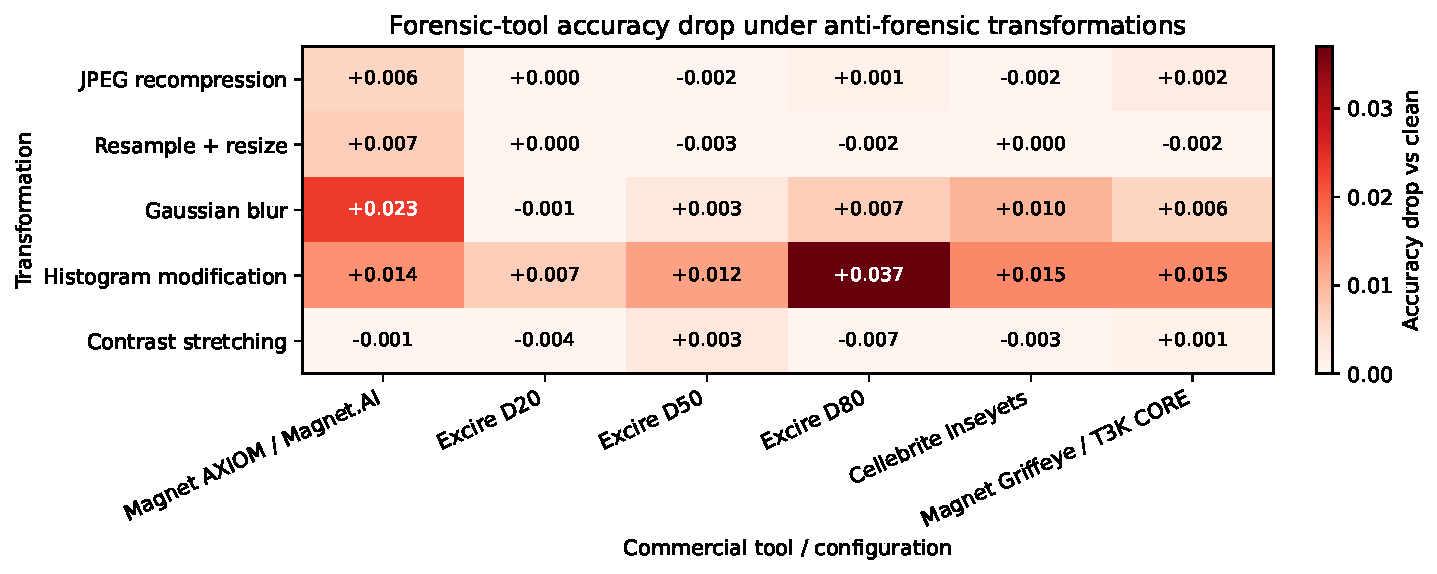
\includegraphics[width=1\textwidth]{images/fig_forensic_tools_anti_forensic_accuracy_drop_heatmap.pdf}
\caption{Accuracy drop of selected black-box software systems under anti-forensic transformations}
\label{fig:results-forensic-tools-antiforensic-drop-heatmap}
\end{figure}

Figure~\ref{fig:results-forensic-tools-antiforensic-drop-heatmap} complements
the tabular interpretation by showing that, for selected software systems,
anti-forensic transformations generally produce limited drops. The most evident
variations are observed for \gls{excirefoto2025} under the \texttt{D80}
configuration with \gls{histogrammodification} and, to a lesser extent, for
\gls{magnetai} under \gls{gaussianblur}. \gls{griffeye}/\gls{t3kcore}
maintains a limited drop, while still exhibiting residual false negatives in
the most critical condition.

The anti-forensic results show generally limited degradation in both proxy
models and selected software systems. This result is important because it
distinguishes the operational effect of plausible transformations from the more
aggressive effect of adversarial perturbations. For EfficientNet-B0, the most
critical condition is \gls{gaussianblur}, which produces 17 induced errors, all
in the \texttt{weapon}\(\rightarrow\)\texttt{non\_weapon} direction. Although
the aggregate drop is limited, this error direction is forensically relevant,
because it corresponds to missed detection of \texttt{weapon} samples.

ResNet18 shows the most marked anti-forensic degradation under
\gls{histogrammodification}, with an accuracy of 0.934 and 39 induced errors.
Unlike EfficientNet-B0, the error pattern is bidirectional: both missed
detections of the \texttt{weapon} class and false \texttt{weapon} flags on
\texttt{non\_weapon} images are present. \gls{clip}, instead, remains
relatively stable with respect to the tested transformations. This confirms
that, in the present protocol, the main criticality of \gls{clip} is not
anti-forensic degradation, but the tendency to map \gls{ood} inputs to the
\texttt{weapon} class.

Selected software systems also show limited aggregate degradation.
\gls{griffeye}/\gls{t3kcore} exhibits the highest aggregate anti-forensic
accuracy, equal to 0.974, followed by \gls{cellebriteinseyets},
\gls{excirefoto2025} under the \texttt{D50} configuration, and \gls{magnetai}.
However, the operational interpretation varies across systems.
\gls{griffeye}/\gls{t3kcore} maintains a very limited \gls{fpr}, but exhibits
residual false negatives under \gls{histogrammodification}.
\gls{cellebriteinseyets} maintains high recall, but with a higher \gls{fpr}
than \gls{griffeye}/\gls{t3kcore}. \gls{magnetai} is more exposed to false
negatives under \gls{gaussianblur}, whereas \gls{excirefoto2025} exhibits a
criticality more attributable to false positive increase under
\gls{histogrammodification}.

\paragraph{Robustness with respect to adversarial perturbations.}

Table~\ref{tab:results-comparative-adversarial} summarizes the adversarial
robustness profile. Unlike anti-forensic transformations, adversarial
perturbations are designed to alter the decision behavior of \gls{ai}-based
systems. For this reason, they produce more heterogeneous and more
model-dependent effects. The results highlight an important distinction among source-model vulnerability
under the defined access assumptions, cross-model transfer across the proxy
architectures, and the operational black-box transfer behavior of the selected
software systems.

\begin{table}[H]
\centering
\caption{Comparison of robustness under adversarial perturbations}
\label{tab:results-comparative-adversarial}
\footnotesize
\renewcommand{\arraystretch}{1.18}
\setlength{\tabcolsep}{3pt}
\begin{tabularx}{\textwidth}{@{}p{2.7cm} p{1.8cm} p{3.1cm} p{2.8cm} X@{}}
\toprule
\textbf{System} &
\textbf{\shortstack{Adversarial\\accuracy/\\drop}} &
\textbf{Most critical condition} &
\textbf{Main error} &
\textbf{Scoped interpretation} \\
\midrule

EfficientNet-B0 &
0.695 / 0.283 &
\gls{sigmazero}; acc. 0.015; drop 0.963 &
963 induced errors; 489 W$\rightarrow$NW and 474 NW$\rightarrow$W &
Most marked proxy vulnerability in the white-box scenario; high clean accuracy
does not guarantee adversarial robustness. \\

ResNet18 &
0.955 / 0.009 &
\gls{fgsm}; acc. 0.918; drop 0.046 &
47 induced errors; 27 W$\rightarrow$NW and 20 NW$\rightarrow$W &
Limited aggregate degradation; the model-dependent results reflect cross-model
transfer, with residual degradation under \gls{fgsm}. The evaluation does not
represent a direct white-box assessment of ResNet18. \\

\gls{clip} &
0.927 / 0.000 &
\gls{fgsm}; acc. 0.914; drop 0.013 &
23 induced errors; 8 W$\rightarrow$NW and 15 NW$\rightarrow$W &
Limited aggregate degradation; the model-dependent results reflect cross-model
transfer and do not demonstrate direct adversarial robustness. The distinct \gls{ood}
assignment behavior must be considered separately. \\

\gls{magnetaxiomtool}/\gls{magnetai} &
0.923 / 0.027 &
\gls{fgsm}; acc. 0.867; \acrshort{fnr} 0.192 &
96 \acrshort{fn} &
Aggregate accuracy decreases by 0.027, while \gls{fgsm} substantially increases
false negatives on the \texttt{weapon} class. \\

\gls{griffeye}/\gls{t3kcore} &
0.969 / 0.009 &
\gls{sigmazero}; acc. 0.959; \acrshort{fnr} 0.074 &
37 \acrshort{fn} &
Highest aggregate normalized accuracy among the selected black-box
configurations under adversarial artifacts; the low \gls{fpr} also reflects the
conservative mapping, while residual degradation remains. \\

\gls{excirefoto2025} \texttt{D50} &
0.904 / 0.040 &
\gls{sigmazero}; acc. 0.742; \acrshort{fpr} 0.442 &
221 \acrshort{fp} &
The principal effect is an increase in firearm-prompt retrievals for
\texttt{non\_weapon} samples rather than systematic concealment of
\texttt{weapon} images. \\

\gls{cellebriteinseyets} &
0.955 / 0.009 &
\gls{fgsm}; acc. 0.918; \acrshort{fnr} 0.106 &
53 \acrshort{fn} &
Limited aggregate degradation under the transferred adversarial artifacts,
with an increase in false negatives especially under \gls{fgsm}. \\

\bottomrule
\end{tabularx}

\vspace{0.4em}
\footnotesize
\textit{Note.} For the proxy models, aggregate values are computed across the
five adversarial perturbations considered. For selected software systems,
values derive from the normalized outputs on the forensic evaluation bundle.
The drop is defined in Section~\ref{sec:results-scope}. W$\rightarrow$NW
indicates transitions from \texttt{weapon} to \texttt{non\_weapon}; \acrshort{fn}
indicates false negatives; \acrshort{fnr} indicates false negative rate; \acrshort{fpr} indicates
false positive rate.
\end{table}

\begin{figure}[H]
\centering
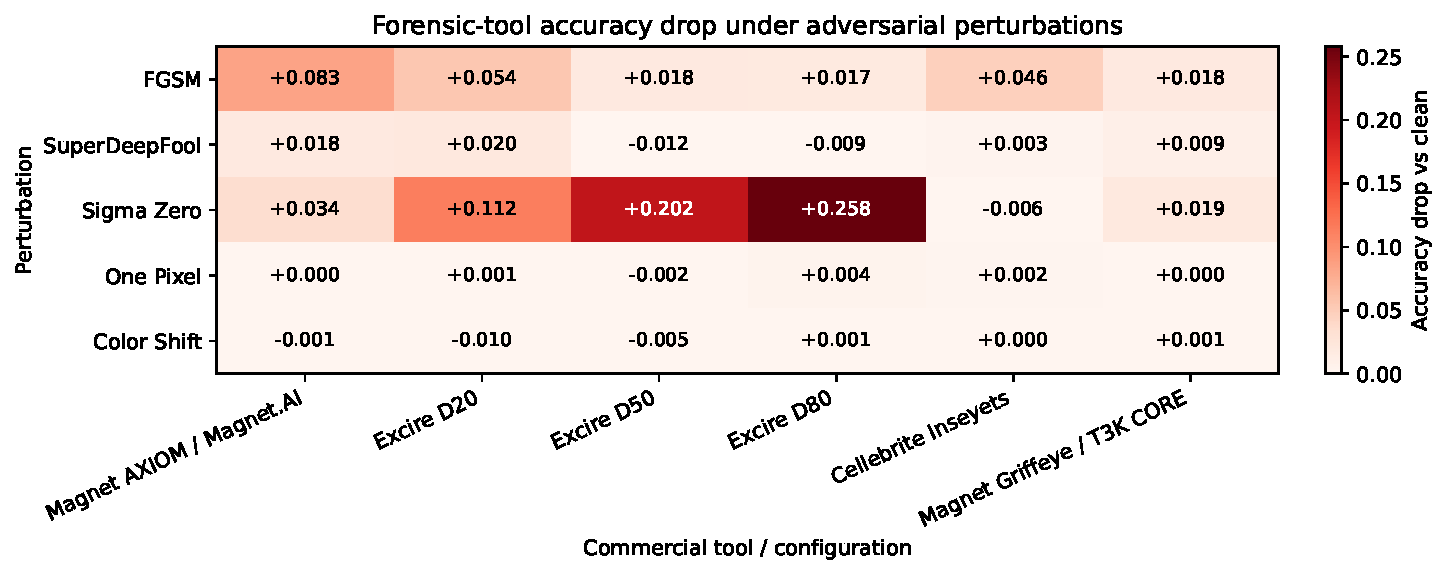
\includegraphics[width=1\textwidth]{images/fig_forensic_tools_adversarial_accuracy_drop_heatmap.pdf}
\caption{Accuracy drop of selected black-box software systems under adversarial perturbations}
\label{fig:results-forensic-tools-adversarial-drop-heatmap}
\end{figure}

Figure~\ref{fig:results-forensic-tools-adversarial-drop-heatmap} shows that the
response of selected software systems to adversarial perturbations is strongly
dependent on the system and configuration. \gls{excirefoto2025} is particularly
sensitive to \gls{sigmazero} under the \texttt{D50} and \texttt{D80}
configurations, whereas \gls{cellebriteinseyets} and
\gls{griffeye}/\gls{t3kcore} show more limited aggregate drops. This result
reinforces the interpretation that the operational robustness of selected
black-box software systems is not uniform, but depends on the type of
observable output, the adopted mapping, and the system configuration.

The adversarial comparison shows that the most severe degradation occurs at the
proxy level, particularly for EfficientNet-B0 under \gls{sigmazero}. The model
moves from a clean accuracy of 0.978 to an accuracy of 0.015, with 963 induced
errors. This result shows, in the considered protocol, that a model may be very
accurate under nominal conditions and, at the same time, extremely fragile with
respect to optimized adversarial perturbations. \gls{fgsm} also produces
significant degradation for EfficientNet-B0, with an accuracy of 0.575 and a
drop of 0.403. The observed vulnerability is therefore not limited to a single
adversarial condition.

ResNet18 and \gls{clip} show a more stable profile in the present experimental
setting. ResNet18 is most affected by \gls{fgsm}, but the drop remains much
lower than that observed for EfficientNet-B0. \gls{clip} is even less degraded
by the tested perturbations. However, this result must be interpreted with caution: the model-dependent
attacks were generated against EfficientNet-B0 rather than against \gls{clip}.
The observed behavior of \gls{clip} therefore represents cross-model transfer
under the evaluated conditions, not direct source-model robustness.
Furthermore, \gls{clip} exhibits a distinct criticality on \gls{ood} inputs.
The observed adversarial stability must consequently not be generalized beyond
the evaluated threat model.

Selected software systems show a different pattern. \gls{magnetai} does not
reproduce the catastrophic degradation observed for EfficientNet-B0 under
\gls{sigmazero}, but is substantially affected by \gls{fgsm}, with a
\gls{fnr} of 0.192. From a forensic perspective, this is a critical error,
because the missed detection of \texttt{weapon} images may lead to the
deprioritization of relevant material.

\gls{excirefoto2025} under the \texttt{D50} configuration instead reacts
differently: \gls{sigmazero} primarily produces an increase in the false
positive rate, equal to 0.442, generating semantic over-triggering rather than
systematic concealment of the \texttt{weapon} class. \gls{cellebriteinseyets}
shows high recall and limited degradation, but maintains a higher false
positive rate than \gls{griffeye}/\gls{t3kcore}. Under the adopted conservative
mapping, \gls{griffeye}/\gls{t3kcore} exhibits the highest aggregate black-box
accuracy and the lowest false positive rate, while still retaining residual
false negatives on the \texttt{weapon} class.

Overall, the comparison among selected software systems does not identify a
single preferable system across all operational criteria, but highlights
different operating profiles. \gls{griffeye}/\gls{t3kcore} exhibits the most
selective profile and the lowest operational noise in terms of false positives;
\gls{cellebriteinseyets} maintains slightly higher recall on the
\texttt{weapon} class; \gls{excirefoto2025} shows behavior strongly dependent
on the retrieval threshold; and \gls{magnetai} exhibits a more conservative
profile but with a higher false negative rate. This heterogeneity shows that
the observed operating profiles of the selected black-box software systems
depend on the software configuration, observable
output, normalization mapping, and role assigned to the analyst in the
workflow.

\paragraph{Threshold sensitivity and black-box interpretation.}

The results of \gls{excirefoto2025} require a separate interpretation, because
the system was evaluated as a semantic retrieval engine and not as a native
forensic classifier. The \texttt{Distance limit} parameter defines the
operational restrictiveness of semantic retrieval. The \texttt{D20}
configuration is restrictive: it reduces false positives and weapon flags on
\gls{ood} inputs, but increases the risk of missed detection of
\texttt{weapon} images. The \texttt{D80} configuration is permissive: it
maximizes recall, but increases false positives and the assignment of
non-relevant or perturbed images to the semantic query related to weapons. The
\texttt{D50} configuration was used as the main comparison point because it
represents an intermediate profile.

This threshold dependence is particularly evident under \gls{sigmazero}. Under
the \texttt{D20} configuration, \gls{excirefoto2025} achieves an accuracy of
0.815, an \acrshort{fnr} of 0.180, and an \acrshort{fpr} of 0.190. Under the \texttt{D50}
configuration, accuracy decreases to 0.742, while \acrshort{fnr} improves to 0.074 and
\acrshort{fpr} increases to 0.442. Under the \texttt{D80} configuration, recall improves
further, but \acrshort{fpr} rises to 0.662. The same software system can therefore support
different forensic priorities depending on the selected operating point:
\texttt{D20} prioritizes the containment of operational noise,
\texttt{D80} prioritizes recall, and \texttt{D50} represents an intermediate
trade-off between false negatives and false positives.

The black-box nature of selected software systems also limits the types of
conclusions that can be drawn. Unlike the proxy models, these systems do not
expose decision boundaries, calibrated scores, architectures, training data, or
internal thresholding logic. Their outputs can therefore be evaluated only at
the operational level, through observable categories, exported tags, retrieval
results, semantic bookmarks, matching rate, non-mappable outputs, false
negatives, false positives, and behavior on \gls{ood} inputs. This limitation
does not represent a weakness of the evaluation protocol; on the contrary, it
reflects the operational condition in which forensic analysts interact with
selected black-box \gls{ai}-assisted software systems.


Figure~\ref{fig:results-operational-risk-summary} summarizes the main
quantitative operating dimensions discussed in the comparative analysis. The
figure
does not encode interpretability as a numerical score, since the distinction
between inspectable proxy models and black-box software systems represents a
methodological condition rather than an experimentally measured variable.

\begin{figure}[H]
    \centering
    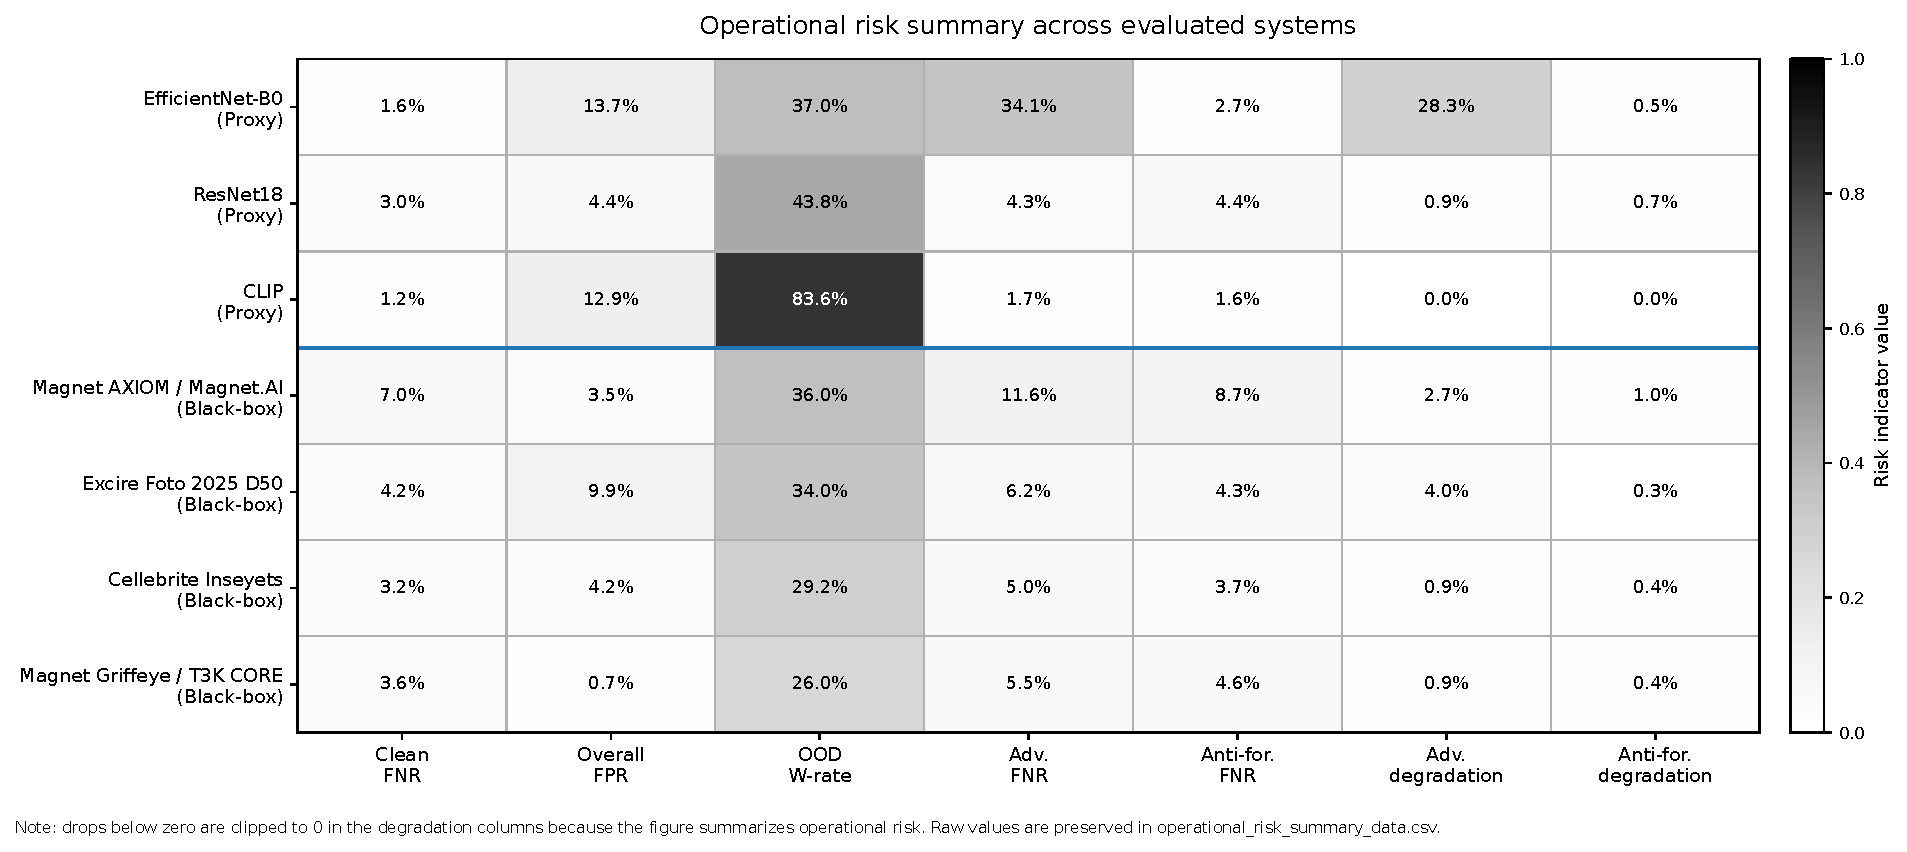
\includegraphics[width=\textwidth]{images/fig_results_operational_risk_summary.pdf}
   \caption[Operational behavior summary across evaluated systems]{Operational
behavior indicators across proxy models and selected black-box software
configurations}
\label{fig:results-operational-risk-summary}

\end{figure}


\begin{flushleft}
\footnotesize
\textit{Note.} Clean \acrshort{fnr} is computed on the unperturbed binary subset. Bundle
\acrshort{fpr} is computed on the complete binary bundle, including clean,
adversarial, and anti-forensic samples and excluding \gls{ood} samples.
Adversarial \acrshort{fnr} and anti-forensic \acrshort{fnr} are aggregated across the corresponding
perturbation families. \acrshort{ood} W-rate reports the proportion of \gls{ood} samples
mapped to the operational \texttt{weapon} class. Accuracy drops are computed
with respect to the clean baseline; slightly negative values are interpreted as
negligible distribution-specific oscillations.
\end{flushleft}

\paragraph{Overall operational interpretation.}

The comparative analysis confirms that robustness in \gls{ai}-assisted forensic
image triage is a multidimensional property. Clean accuracy measures nominal
performance, but it does not capture \gls{ood} weapon assignment behavior,
sensitivity to
perturbations, false negative rates, semantic over-triggering, or the effect of
thresholds in black-box systems. In \gls{df} workflows, these dimensions are at
least as relevant as aggregate accuracy, because they influence analyst
attention, content prioritization, and the manual review strategy.

Three main findings emerge. First, proxy models are useful because they make
controlled degradation patterns observable and allow confidence shift, induced
errors, and error direction to be measured. However, their behavior cannot be
automatically transferred to selected software systems because their internal
mechanisms for classification, tagging, retrieval, and semantic-bookmark
generation are inaccessible. Second, selected software systems show differentiated operating profiles:
some privilege recall, others reduce false positives, and others depend strongly
on the retrieval configuration or adopted semantic mapping. Third, \gls{ood}
behavior remains a distinct evaluation dimension because weapon-oriented outputs
on this branch may increase analyst workload or affect prioritization even
though they are not supervised binary errors.

Overall, the results support a cautious interpretation of \gls{ai}-based
automation in forensic contexts. The evaluated systems can provide useful
support for triage, prioritization, and large-scale review of multimedia
content. However, their outputs must not be treated as conclusive evidence or
as substitutes for expert validation. In particular, missed detections of
\texttt{weapon} images, high-confidence \gls{ood} assignments, and threshold-dependent
errors must be explicitly documented when \gls{ai}-assisted software systems
are used in forensic workflows. The \gls{fairlab} protocol responds to this
need by combining frozen datasets, traceable manifests, hash-based
reproducibility, controlled perturbation families, black-box output
normalization, and manual auditability of the final interpretation.

% ─────────────────────────────────────────────────────────────────────────────
\section{Explainability Analysis and Representative Failure Cases}
\label{sec:results-explainability}
% ─────────────────────────────────────────────────────────────────────────────

The \gls{xai} analysis was used as a qualitative and diagnostic tool to connect
the aggregate metrics discussed in the previous sections to a restricted set of
representative cases. It does not constitute a primary robustness metric and
does not replace quantitative measures of accuracy, confidence, false positives,
and false negatives. Its role is instead to support the operational
interpretation of selected behaviors observed in the proxy model, by
showing the spatial distribution of attribution magnitude for the selected
model output in specific success or failure scenarios.

The attribution maps were generated using \gls{ig} applied to the white-box
EfficientNet-B0 proxy model, with the model-predicted class as the attribution
target, indicated in the experimental files as \texttt{predicted\_label}.
This choice associates each visualization with the output actually produced
by the model rather than with the reference operational assignment. In erroneous
cases, the map therefore represents attribution magnitude for the incorrect
predicted class.

The generated maps must not be interpreted as direct explanations of the
behavior of \gls{magnetaxiomtool}/\gls{magnetai},
\gls{excirefoto2025}, \gls{cellebriteinseyets}, or
\gls{griffeye}/\gls{t3kcore}, which remain black-box systems in the context of
this evaluation. Rather, they provide a controlled diagnostic reference, limited
to the white-box proxy model, and support discussion of selected proxy-model
behaviors in a \gls{df}
\textit{human-in-the-loop} context.

The \gls{xai} figures reported in this section follow the generation and
selection procedure documented in
Section~\ref{subsec:implementation-explainability}: input image, \gls{ig}
heatmap, attribution overlay on the original image, and mask of the locations
with the largest attribution magnitudes. The attribution mask must not be interpreted as a
semantic segmentation,
object-level annotation, or causal explanation. It visualizes the locations with
the largest absolute attribution magnitudes under the adopted baseline and
target. Similarly, the reported score is the proxy model's maximum
predicted-class probability and is not treated as calibrated.

As documented in Section~\ref{subsec:implementation-explainability}, the
retained historical figures were generated using 32 integration steps and are
interpreted exclusively as qualitative diagnostic visualizations. No strict
numerical convergence claim is made for these assets.

Table~\ref{tab:results-xai-cases} summarizes the five cases selected for the
qualitative analysis. The selection covers one correct case on a clean input,
one false negative on a clean input, one \gls{ood} case assigned to
\texttt{weapon}, one false negative produced by an anti-forensic transformation,
and one high-confidence adversarial false positive.

\begin{table}[htbp]
\centering
\small
\renewcommand{\arraystretch}{1.15}
\setlength{\tabcolsep}{4pt}
\caption{Representative cases selected for the qualitative analysis of EfficientNet-B0 using \gls{ig}}
\label{tab:results-xai-cases}
\begin{tabularx}{\textwidth}{@{}p{0.17\textwidth} p{0.15\textwidth} p{0.13\textwidth} p{0.13\textwidth} X@{}}
\toprule
\textbf{Identifier} &
\textbf{Scenario} &
\textbf{Reference state} &
\textbf{Prediction} &
\textbf{Operational role} \\
\midrule

\texttt{xai\_case\_0001} &
\texttt{clean} &
\texttt{weapon} &
\texttt{weapon} &
Correct case on a clean input, used as a reference for observing coherent
attribution behavior. \\

\texttt{xai\_case\_0006} &
\texttt{clean} &
\texttt{weapon} &
\texttt{non\_weapon} &
False negative on a clean input, representative of missed detection in the
absence of perturbations. \\

\texttt{xai\_case\_0009} &
\texttt{ood} &
\texttt{ood} &
\texttt{weapon} &
\gls{ood} input assigned to \texttt{weapon}, representing a closed-set
assignment on the separate evaluation branch. \\

\texttt{xai\_case\_0010} &
\gls{histogrammodification} &
\texttt{weapon} &
\texttt{non\_weapon} &
Anti-forensic false negative, representative of the effects of low-level visual
manipulations. \\

\texttt{xai\_case\_0015} &
\gls{sigmazero} &
\texttt{non\_weapon} &
\texttt{weapon} &
High-score adversarial false positive, representative of the unreliability of
the maximum predicted-class probability as a stand-alone reliability indicator. \\

\bottomrule
\end{tabularx}
\vspace{0.4em}
\footnotesize
\textit{Note.} For \texttt{xai\_case\_0009}, \texttt{ood} denotes the separate
\gls{ood} evaluation branch and not a third supervised class.
\end{table}

\XAIcaseFigureMaskGrid
{fig:xai-case1-clean-correct}
{Correct case on a clean input \texttt{xai\_case\_0001}. The EfficientNet-B0
proxy model correctly classifies a \texttt{clean} image with reference
operational assignment \texttt{weapon} as \texttt{weapon}}
{images/fig_xai_case1_clean_correct_input.png}
{images/fig_xai_case1_clean_correct_heatmap.png}
{images/fig_xai_case1_clean_correct_overlay.png}
{images/fig_xai_case1_clean_correct_top10_mask.png}
{\textbf{scenario}: \texttt{clean};
\textbf{reference state}: \texttt{weapon};
\textbf{prediction}: \texttt{weapon};
\textbf{confidence}: 1.000}

The first case, shown in Figure~\ref{fig:xai-case1-clean-correct}, provides a
qualitative reference in which the model prediction is consistent with the
reference operational assignment. The image belongs to the \texttt{clean}
scenario, its reference operational
assignment is \texttt{weapon}, and EfficientNet-B0 also predicts
\texttt{weapon}, with a maximum predicted-class probability of 1.000. In this
case, the \gls{ig} map supports inspection of whether larger attribution
magnitudes overlap the visually salient object region or are concentrated on
background and contextual elements. This example does not, by
itself, demonstrate the general reliability of the model, but serves as a
reference case against which the subsequent failures can be compared.

\XAIcaseFigureMaskGrid
{fig:xai-case2-clean-false-negative}
{False negative on a clean input \texttt{xai\_case\_0006}. A \texttt{clean}
image with reference operational assignment \texttt{weapon} is classified as
\texttt{non\_weapon}}
{images/fig_xai_case2_clean_false_negative_input.png}
{images/fig_xai_case2_clean_false_negative_heatmap.png}
{images/fig_xai_case2_clean_false_negative_overlay.png}
{images/fig_xai_case2_clean_false_negative_top10_mask.png}
{\textbf{scenario}: \texttt{clean};
\textbf{reference state}: \texttt{weapon};
\textbf{prediction}: \texttt{non\_weapon};
\textbf{confidence}: 0.692}

The second case, reported in
Figure~\ref{fig:xai-case2-clean-false-negative}, is relevant because the error
occurs on a clean input, without adversarial perturbations or anti-forensic
transformations. The image has the reference operational assignment
\texttt{weapon}, but
EfficientNet-B0 classifies it as \texttt{non\_weapon} with a maximum
predicted-class probability of 0.692.
In a \gls{df} workflow, this type of error may have a direct operational
consequence because a false negative may prevent a potentially relevant image
from being prioritized during automated triage.

The corresponding \gls{ig} map makes it possible to inspect whether the
largest attribution magnitudes are localized on the object region or distributed
across contextual elements. This case shows that good aggregate performance on \texttt{clean} data does not eliminate
the need for human assessment, especially when the automatic result is used to
filter or rank large volumes of images in an investigative context.

\XAIcaseFigureMaskGrid
{fig:xai-case3-ood-as-weapon}
{\gls{ood} case \texttt{xai\_case\_0009}. An \gls{ood} input is
assigned to \texttt{weapon} with a high maximum predicted-class probability}
{images/fig_xai_case3_ood_as_weapon_input.png}
{images/fig_xai_case3_ood_as_weapon_heatmap.png}
{images/fig_xai_case3_ood_as_weapon_overlay.png}
{images/fig_xai_case3_ood_as_weapon_top10_mask.png}
{\textbf{scenario}: \texttt{ood};
\textbf{reference state}: \texttt{ood};
\textbf{prediction}: \texttt{weapon};
\textbf{confidence}: 0.999}

The third case, shown in Figure~\ref{fig:xai-case3-ood-as-weapon}, differs from
an ordinary false positive because the sample belongs to the separate \gls{ood}
evaluation branch and has no binary reference assignment. EfficientNet-B0 maps
it to \texttt{weapon} with a maximum predicted-class probability of 0.999.
The \gls{ood} branch includes borderline, distributionally atypical, degraded,
synthetic, or semantically out-of-task cases rather than a homogeneous class of
realistic negatives.

The \gls{ig} visualization shows whether larger attribution magnitudes for
the predicted \texttt{weapon} output are localized or distributed across the
input. It does not establish that the highlighted regions correspond to
firearm-specific features. From a methodological perspective, this case
supports the choice to preserve \texttt{ood} as a separate dataset and evaluation branch, rather than treating
it as a third supervised class or merging all inputs outside the
\texttt{weapon} class into the \texttt{non\_weapon} class.

\XAIcaseFigureMaskGrid
{fig:xai-case4-antiforensic-failure}
{Anti-forensic false negative \texttt{xai\_case\_0010}. A \texttt{weapon} image
subjected to \gls{histogrammodification} is classified as
\texttt{non\_weapon}}
{images/fig_xai_case4_antiforensic_failure_input.png}
{images/fig_xai_case4_antiforensic_failure_heatmap.png}
{images/fig_xai_case4_antiforensic_failure_overlay.png}
{images/fig_xai_case4_antiforensic_failure_top10_mask.png}
{\textbf{scenario}: \gls{histogrammodification};
\textbf{reference state}: \texttt{weapon};
\textbf{prediction}: \texttt{non\_weapon};
\textbf{confidence}: 0.852}

The fourth case, reported in
Figure~\ref{fig:xai-case4-antiforensic-failure}, concerns an anti-forensic
transformation based on \gls{histogrammodification}. The reference operational
assignment remains \texttt{weapon}, but the model predicts
\texttt{non\_weapon} with a maximum predicted-class probability of
0.852. The case is relevant because the transformation is not an adversarial
perturbation optimized against a differentiable model. It is instead a
low-level visual manipulation that affects tonal distribution, contrast, and
the local representation of image structures.

The \gls{ig} map enables comparison of the attribution distribution observed
for this transformed input, but it does not isolate the causal mechanism through
which histogram modification changed the prediction. From an operational
perspective, this failure suggests that transformations that may remain visually recognizable to human analysts can
nevertheless compromise automated classification. In a forensic pipeline, this
reinforces the need not to treat the classifier output as autonomous evidence,
but as support to be critically verified.

\XAIcaseFigureMaskGrid
{fig:xai-case5-adversarial-high-confidence-failure}
{High-confidence adversarial false positive \texttt{xai\_case\_0015}. A
\texttt{non\_weapon} image perturbed using \gls{sigmazero} is classified as
\texttt{weapon}}
{images/fig_xai_case5_adversarial_high_conf_failure_input.png}
{images/fig_xai_case5_adversarial_high_conf_failure_heatmap.png}
{images/fig_xai_case5_adversarial_high_conf_failure_overlay.png}
{images/fig_xai_case5_adversarial_high_conf_failure_top10_mask.png}
{\textbf{scenario}: \gls{sigmazero};
\textbf{reference state}: \texttt{non\_weapon};
\textbf{prediction}: \texttt{weapon};
\textbf{confidence}: 1.000}

The fifth case, shown in
Figure~\ref{fig:xai-case5-adversarial-high-confidence-failure}, represents a
high-confidence adversarial false positive. The image has the reference
operational assignment \texttt{non\_weapon}, but, after the \gls{sigmazero} perturbation, it is
classified as \texttt{weapon} with a maximum predicted-class probability of
1.000. For the purposes of this thesis, this case is particularly significant because it separates two
concepts that may be incorrectly conflated in an operational workflow: the
maximum predicted-class probability and the forensic reliability of the
prediction.

The \gls{ig} visualization provides a diagnostic representation of
attribution magnitude for the incorrect predicted class, but it must not be
interpreted as a complete explanation of the attack mechanism. Its value lies
in making a high-score failure directly observable and showing that a maximum
predicted-class probability of 1.000 does not establish operational
reliability. In an investigative context, this
result supports the need to maintain the \textit{human-in-the-loop} paradigm,
especially when \gls{ai}-based systems are used to prioritize sensitive or
potentially relevant content.

Overall, the five selected cases show that \gls{xai} analysis can provide a
useful interpretive contribution, provided that its role remains properly
delimited. The correct case on a clean input serves as a qualitative reference
for coherent attribution behavior; the false negative on a clean input shows
that missed detection can occur even in the absence of manipulation; the
\gls{ood} case documents a closed-set \texttt{weapon} assignment on the
separate evaluation branch; the anti-forensic case shows that low-level visual
transformations can alter the automatic decision; and the high-confidence
adversarial case shows that confidence cannot be assumed as a sufficient
indicator of operational reliability.

For these reasons, \gls{xai} analysis is considered in this thesis as support
for understanding representative cases and not as autonomous evidence of system
robustness. It makes selected behaviors of the EfficientNet-B0 proxy model more
transparent, but it does not automatically extend its conclusions to selected
black-box software systems. In a \gls{df} pipeline, visualizations based on
\gls{ig} must therefore be interpreted as instruments supporting review,
evaluation, and critical discussion of the results, while preserving the central
role of the human analyst in the final assessment.


% ─────────────────────────────────────────────────────────────────────────────
\section{Operational Interpretation and Experimental Limitations}
\label{sec:results-limitations}
% ─────────────────────────────────────────────────────────────────────────────

The results show that the operational robustness of \gls{ai}-based systems for
forensic image classification and triage cannot be inferred from clean accuracy
alone. Interpretation must jointly consider the direction of the errors,
behavior on \gls{ood} inputs, degradation under manipulated conditions,
threshold- or mapping-dependent trade-offs, and the extent to which the output
remains auditable and subject to human verification.

False negatives and false positives have different operational consequences. A
false negative on the \texttt{weapon} class may prevent potentially relevant
content from being prioritized for review. A false positive may instead
increase analyst workload and dilute
prioritization. A \texttt{weapon} assignment on an \gls{ood} input is not a
binary error, but may produce similar workload or prioritization effects.
Aggregate accuracy therefore provides only a partial description of the
observed operating profile.

The parallel comparison also demonstrates that nominally strong systems may
fail under different conditions. EfficientNet-B0 achieves the highest clean
accuracy among the proxy models but undergoes severe white-box degradation
under \gls{sigmazero} and substantial degradation under \gls{fgsm}. The
selected black-box software systems do not exhibit the same collapse on those
artifacts, but their observable outputs reveal other limitations, including
missed detections, false-positive workload, configuration sensitivity, and
non-zero \gls{ood} weapon-flag rates. These differences reinforce the need to
evaluate systems through multiple operational conditions rather than a single
clean benchmark.

Several limitations define the scope of the findings.

\begin{itemize}
    \item The frozen dataset contains 1\,500 manually selected images and does
    not represent the full diversity of firearm-related, non-firearm, and
    \gls{ood} imagery encountered in operational investigations.
    Selection was performed by a single reviewer; no inter-rater agreement was
    measured.

    \item The source distribution is not uniform. In particular, the
    \texttt{non\_weapon} branch is predominantly derived from
    \texttt{05\_deepweb}. Source-specific regularities may therefore influence
    some observed results despite the source-aware fold construction.

    \item The four model-dependent adversarial attacks were generated against
    fold-aware EfficientNet-B0 checkpoints. The resulting cross-model and
    black-box analyses measure transfer behavior of those artifacts, not a
    complete attack space optimized independently against every evaluated
    system.

    \item The adversarial and anti-forensic suites are finite and use one frozen
    parameterization per condition. Different budgets, severities, image
    encodings, attack implementations, or transformation combinations may
    produce different robustness profiles.

    \item The proxy architectures are transparent experimental references and
    must not be interpreted as reconstructions of the internal models used
    by the selected software systems.

    \item Black-box results depend on the evaluated software versions, enabled
    functions, export formats, and explicit normalization rules. The conservative
    firearm-bookmark mapping adopted for \gls{griffeye}/\gls{t3kcore} and the
    distance setting adopted for \gls{excirefoto2025} directly affect the
    observed balance between missed detections and false-positive workload.

    \item Proxy-model \gls{ood} rates aggregate five predictions per image,
    whereas black-box rates use one normalized decision per image. The resulting
    proportions support parallel descriptive comparison but do not constitute
    identical statistical observations.

    \item The retained \gls{xai} analysis is limited to five representative
    EfficientNet-B0 cases. The historical assets were generated with 32
    integration steps and are used only for qualitative interpretation; no
    strict convergence claim is made, and the findings cannot be extended to
    the selected black-box software systems.

    \item The embedded-metadata audit identified a small residual information
    channel in the blind bundle. The leave-out analysis indicates limited
    quantitative influence on the reported aggregate metrics. However, the frozen
    protocol did not include a separate metadata-neutralized comparison bundle, and
    the corresponding analysis therefore remains limited to the
    metadata-preserving bundle used in the experiment.
\end{itemize}

These limitations delimit the conditions under which the experimental
conclusions are supported. The chapter therefore
provides a protocol-specific assessment of operational robustness rather than
a software-system certification, universal robustness ranking, or
evidentiary validation of automated outputs.

The practical implication is that automated image-analysis systems should be
used as traceable triage support within a \textit{human-in-the-loop} workflow.
Their outputs should remain associated with the source item, system version,
configuration, observable mapping, and relevant uncertainty or limitation. In
particular, missed detections, configuration-dependent behavior, high-confidence
failures, and \gls{ood} assignments must remain visible to the analyst rather
than being hidden behind a single aggregate score.


% ----------------- Chapter 7: Conclusions and Future Work ----------------------
% ─────────────────────────────────────────────────────────────────────────────
\chapter{Conclusions, Limitations, and Future Work}
\label{chap:conclusions}
% ─────────────────────────────────────────────────────────────────────────────


% ─────────────────────────────────────────────────────────────────────────────
\section{Summary of the Research}
\label{sec:conclusions-summary}
% ─────────────────────────────────────────────────────────────────────────────

This thesis investigated the operational robustness of \gls{ai}-based systems
used for automated image classification and triage in forensic contexts. The
study was motivated by the observation that nominal performance on clean and
well-structured data does not fully characterize the behavior of systems that
may be applied to heterogeneous, degraded, distributionally different, or
deliberately manipulated digital evidence.

Within a \gls{df} workflow, classification errors may affect not only
technical performance but also the prioritization of material, the allocation
of analyst attention, and the effectiveness of the subsequent human review
process. A missed \texttt{weapon} image may fail to receive appropriate
priority, whereas an incorrect positive assignment may increase the volume of
irrelevant material requiring examination.

The research therefore adopted an operational perspective. Adversarial
attacks, anti-forensic transformations, and \gls{ood} inputs were treated as
distinct experimental conditions for examining system behavior beyond the
clean baseline. The objective was not to construct a conventional
\gls{advml} benchmark or to identify a universally superior system. Instead,
the study assessed whether nominal performance remained stable when the input
conditions changed and examined the resulting consequences for forensic
triage.

The experimental design combined two complementary evaluation levels. The
first comprised three transparent proxy models: \gls{efficientnetb0}, \gls{resnet18}, and
a \gls{clip}-based model consisting of a frozen visual encoder and a supervised
binary classification head. These models provided access to predicted classes,
maximum predicted-class probabilities, confusion matrices,
clean-to-perturbed error transitions, and internal gradients.

The second evaluation level comprised
\gls{magnetaxiomtool}/\gls{magnetai},
\gls{griffeye}/\gls{t3kcore},
\gls{excirefoto2025}, and
\gls{cellebriteinseyets}. These selected black-box software systems were
evaluated exclusively through the outputs observable to the analyst and through
explicitly documented normalization rules. The proxy models were not intended
to reproduce, approximate, or explain the proprietary internal models used by
the selected software systems.

A central methodological feature was the use of the same frozen source
population at both evaluation levels. The dataset comprised 1\,500 source
images: 500 \texttt{weapon} images, 500 \texttt{non\_weapon} images, and a
separate 500-image \gls{ood} branch. Adversarial and anti-forensic artifacts
were generated exclusively from the 1\,000-image binary subset.

The resulting forensic evaluation bundle contained 11\,500 logical items:
1\,000 clean binary inputs, 500 clean \gls{ood} inputs, 5\,000 adversarial
artifacts, and 5\,000 anti-forensic artifacts. The 10\,000 perturbed artifacts
remain derived versions of the same 1\,000 binary source images and do not
represent independent underlying cases.

The selected black-box configurations produced one normalized decision for
every bundle item, whereas the proxy-model pipeline preserved the fold-aware
evaluation design described in Chapter~\ref{chap:implementation}. This common
experimental basis made it possible to compare observable operating profiles
without assuming architectural or semantic equivalence among the evaluated
systems.

The complete procedure was formalized through the \gls{fairlab} protocol.
\gls{fairlab} is not a new classifier or standalone software platform. It is a
task-specific evaluation protocol connecting dataset construction, human
semantic validation, deterministic partitioning, proxy-model evaluation,
perturbation generation, blind-bundle construction, black-box output
normalization, quantitative metrics, qualitative explainability analysis, and
traceability controls.

Its purpose is to make operational robustness experimentally observable while
supporting procedural reproducibility and artifact-level auditability. The
protocol preserves the relationships among source images, derived artifacts,
model predictions, proprietary software outputs, normalized decisions, metrics,
and reporting assets.

The principal conclusion is that robustness cannot be inferred from clean
accuracy alone. It must be evaluated as a contextual property of a specific
system version, configuration, task definition, input population, output
mapping, and threat model.

Automated image-analysis outputs may provide useful support for forensic
triage, but they must remain traceable, reviewable, and subordinate to expert
assessment
\cite{costantini2019digital,sanna2024preliminary,sanna2025pixelperfect}.

% ─────────────────────────────────────────────────────────────────────────────
\section{Answers to the Research Questions}
\label{sec:conclusions-research-questions}
% ─────────────────────────────────────────────────────────────────────────────

\paragraph{\textbf{RQ1. To what extent do the transparent proxy models maintain
their clean-baseline performance under the separate \gls{ood}, adversarial,
and anti-forensic conditions?}}

The proxy models maintain their clean-baseline performance only to a
condition-dependent extent. All three architectures achieve comparatively
strong clean performance, with accuracies of 0.978 for \gls{efficientnetb0}, 0.964
for \gls{resnet18}, and 0.927 for the \gls{clip}-based proxy. These nominal results do
not remain uniformly representative under the other evaluation branches.

The five anti-forensic transformations generally produce smaller aggregate
accuracy variations than the strongest adversarial attacks. The largest
anti-forensic accuracy reduction among the proxy models is 0.030 for \gls{resnet18}
under \gls{histogrammodification}. Even where aggregate accuracy remains
unchanged or increases, however, clean-correct samples may become incorrect.
Anti-forensic robustness must therefore be interpreted through both aggregate
metrics and directional error transitions.

The direct-target adversarial conditions produce the most substantial
degradation. \gls{efficientnetb0} accuracy decreases from 0.978 to 0.575 under
\gls{fgsm} and to 0.015 under \gls{sigmazero}. The corresponding results show
that strong clean performance does not imply robustness to attacks optimized
against the evaluated model.

The separate \gls{ood} branch exposes an additional behavior that cannot be
predicted from clean binary accuracy. The fold-aggregated weapon assignment
rates are 0.3696 for \gls{efficientnetb0}, 0.4376 for \gls{resnet18}, and 0.8356 for the
\gls{clip}-based proxy. These values describe forced closed-set assignments and
not supervised correctness.

The proxy models therefore preserve nominal behavior under some frozen
conditions but not across the complete evaluation. Clean performance,
anti-forensic sensitivity, direct adversarial vulnerability, and \gls{ood}
assignment behavior remain distinct dimensions
(Sections~\ref{sec:results-clean-baseline}--\ref{sec:results-adversarial}).

\paragraph{\textbf{RQ2. How do direct source-model attacks,
cross-architecture transfer, and the model-agnostic \gls{colorshift} condition
differ in their effects on the evaluated proxy models?}}

The direct source-model attacks produce substantially larger effects than the
observed cross-architecture transfer. The four model-dependent attacks were
generated against fold-specific \gls{efficientnetb0} checkpoints. Their evaluation
on \gls{efficientnetb0} therefore represents direct-target assessment, whereas
their evaluation on \gls{resnet18} and the \gls{clip}-based proxy measures empirical
transfer.

The clearest direct-target failure is produced by \gls{sigmazero}, which
reduces \gls{efficientnetb0} accuracy to 0.015 and renders 963 of the 978
clean-correct samples incorrect. \gls{fgsm} reduces accuracy to 0.575 and
introduces 406 errors among clean-correct samples, predominantly in the
\texttt{weapon}-to-\texttt{non\_weapon} direction.

The same frozen artifacts produce more limited and heterogeneous effects on
the non-target architectures. The largest transferred degradation is observed
under \gls{fgsm}: \gls{resnet18} accuracy decreases from 0.964 to 0.918, whereas the
\gls{clip}-based proxy decreases from 0.927 to 0.914. Transferred
\gls{sigmazero} artifacts do not reproduce the direct-target collapse and
instead coexist with small aggregate accuracy increases and limited numbers of
new individual errors.

These results demonstrate that transferability must be measured rather than
assumed. Limited transfer does not establish direct robustness of \gls{resnet18} or
the \gls{clip}-based proxy because no matched attacks were optimized
independently against those architectures.

\gls{colorshift} follows a separate experimental rationale. It is deterministic
and model-agnostic and does not use gradients, parameters, scores, or
checkpoints. Its effects are comparatively limited and are interpreted as
condition-specific induced errors rather than direct or transferred attack
success
(Section~\ref{sec:results-adversarial}).

\paragraph{\textbf{RQ3. How do the selected black-box software systems respond
to the same frozen experimental corpus, and how do observable output semantics
and configuration choices affect the resulting operational profiles?}}

The selected black-box software systems produce heterogeneous operating
profiles even though they process the same frozen forensic evaluation bundle.
Their outputs are not internally equivalent: the evaluated decisions derive
from tags, bookmarks, exported classification labels, or semantic-retrieval
membership. The resulting metrics are therefore conditional on the explicit
normalization rule adopted for each configuration.

Under the frozen protocol, \gls{griffeye}/\gls{t3kcore} achieves a
bundle-weighted accuracy of 0.972 and an \gls{fpr} of 0.007. This selective
profile is inseparable from the conservative decision to treat only the
\texttt{CORE/Violence/Firearm} bookmark as a primary positive result.

\gls{cellebriteinseyets} produces a comparatively balanced profile, with
bundle accuracy, weapon recall, and weapon precision all close to 0.958,
together with similar overall false-negative and false-positive rates.

\gls{magnetaxiomtool}/\gls{magnetai} achieves a bundle accuracy of 0.933 and
an \gls{fnr} of 0.099. Its condition-level results show increased
missed-target exposure under transferred \gls{fgsm} artifacts and
\gls{gaussianblur}.

The three \gls{excirefoto2025} configurations provide the clearest evidence of
configuration sensitivity. On clean inputs, moving from \texttt{D20} to
\texttt{D80} reduces the \gls{fnr} from 0.120 to 0.014, while increasing the
\gls{fpr} from 0.026 to 0.156. The corresponding \gls{ood} weapon assignment
rate increases from 0.238 to 0.522. Under transferred \gls{sigmazero}
artifacts, the same change reduces the \gls{fnr} from 0.180 to 0.024 but
increases the \gls{fpr} from 0.190 to 0.662.

The results therefore do not support a universal ranking. More restrictive
configurations may reduce false-positive review workload while increasing
missed detections. More permissive configurations may reduce missed-target risk
while routing substantially more \texttt{non\_weapon} and \gls{ood} material
to the firearm-oriented review category.

Observable output semantics, category selection, retrieval settings, software
versions, enabled processing functions, and normalization rules are therefore
part of the evaluated operating profile
(Section~\ref{sec:results-commercial}).

\paragraph{\textbf{RQ4. Which error transitions, robustness degradations,
\gls{ood} assignment behaviors, and unknown output states are most relevant
to forensic triage and continued human review?}}

The most relevant error transition is
\texttt{weapon}\(\rightarrow\)\texttt{non\_weapon}, because it may prevent
potentially relevant firearm-oriented content from receiving appropriate review
priority. The opposite transition,
\texttt{non\_weapon}\(\rightarrow\)\texttt{weapon}, remains operationally
important because it increases analyst workload and may dilute prioritization.

Aggregate degradation must be interpreted jointly with these directions. The
\gls{efficientnetb0} \gls{sigmazero} result demonstrates a near-total direct-target
collapse involving both missed targets and increased false-positive workload.
Transferred \gls{fgsm} artifacts instead produce particularly relevant
false-negative burdens for Magnet.AI and Cellebrite Inseyets, whereas Excire
\texttt{D50} under transferred \gls{sigmazero} primarily exhibits an expansion
of false-positive semantic retrievals.

The \gls{ood} results identify a separate operational risk. An \gls{ood} input
assigned to \texttt{weapon} is not a supervised false positive, but it may
still be prioritized for review and increase workload. The evaluated proxy
models and all six black-box configurations produce non-zero weapon assignment
rates on the separate \gls{ood} branch.

Maximum predicted-class probabilities also require cautious interpretation.
The representative \gls{sigmazero} failure shows that an incorrect prediction
may be associated with a maximum probability of 1.000. Such a value does not
establish calibrated certainty, correctness, or forensic reliability.

No \texttt{unknown} normalized output occurs in the canonical 69\,000-decision
black-box result population. Consequently, unknown outputs were not an observed
failure mode in the frozen evaluation. Their explicit handling remains
methodologically necessary for future software versions, alternative exports,
or incomplete normalization cases.

The principal operational requirements are therefore systematic human review,
task-specific validation, documentation of software and model versions,
explicit recording of configurations and output mappings, preservation of the
links between source items and normalized decisions, and separate reporting of
missed-target risk, false-positive workload, and \gls{ood} assignment behavior
(Sections~\ref{sec:results-comparative} and
\ref{sec:results-limitations}).


% ─────────────────────────────────────────────────────────────────────────────
\section{Main Contributions}
\label{sec:conclusions-contributions}
% ─────────────────────────────────────────────────────────────────────────────

The contribution of this thesis is articulated across four closely connected
dimensions.

First, the thesis formalizes \gls{fairlab} as an integrated methodological
protocol for evaluating the operational robustness of \gls{ai}-based
image-analysis systems in \gls{df}. The protocol extends evaluation beyond
clean classification accuracy and connects human-validated dataset
construction, deterministic partitioning, transparent proxy-model analysis,
adversarial attacks, anti-forensic transformations, a separate \gls{ood}
branch, black-box software evaluation, output normalization, explainability,
and traceability controls.

The methodological contribution lies in the coordinated application of these
components within a single reproducible and auditable process. \gls{fairlab}
is not proposed as a new classifier, defensive mechanism, or standalone
forensic software platform. It provides a structured procedure through which
system behavior can be examined under controlled but operationally relevant
conditions.

Second, the work establishes a common frozen experimental basis for the
parallel evaluation of transparent proxy models and selected black-box software
systems. The source population contains three equally sized branches,
comprising 500 \texttt{weapon} images, 500 \texttt{non\_weapon} images, and
500 images reserved for the separate \gls{ood} analysis.

The 1\,000-image binary subset was used to generate five adversarial or
adversarial-style artifact populations and five anti-forensic artifact
populations. Together with the clean binary and \gls{ood} images, these
derivatives form the 11\,500-item forensic evaluation bundle.

The 10\,000 perturbed artifacts remain linked to their 1\,000 binary source
images and are not treated as independent underlying cases. This structure
allows clean and manipulated behavior to be compared while preserving the
identity and provenance of each source--condition combination.

Third, the thesis integrates transparent model evaluation with operational
black-box assessment without assuming architectural equivalence between the two
levels.

\gls{efficientnetb0}, \gls{resnet18}, and the \gls{clip}-based proxy provide inspectable
experimental references. They allow direct access to fold-specific
checkpoints, predicted classes, maximum predicted-class probabilities,
confusion matrices, matched clean-to-perturbed transitions, and internal
gradients.

The selected black-box systems instead expose heterogeneous operational
outputs. For \gls{magnetaxiomtool}/\gls{magnetai}, the observable output is the
\texttt{Possible weapons} tag, whereas
\gls{griffeye}/\gls{t3kcore} exposes the
\texttt{CORE/Violence/Firearm} bookmark.

The operational output adopted for \gls{excirefoto2025} is membership in the
union of eight firearm-oriented semantic-query result sets. For
\gls{cellebriteinseyets}, the evaluation uses the exported \texttt{Armi},
\texttt{Pistola}, and \texttt{Fucile} classification labels.

These outputs were normalized into a common operational
\texttt{weapon}/\texttt{non\_weapon} representation while keeping the
\gls{ood} branch analytically separate. The explicit normalization rules make
the comparison reproducible without implying that the selected systems
implement the same internal taxonomy or classification task.

The same model-dependent artifacts generated against fold-specific
\gls{efficientnetb0} checkpoints were subsequently evaluated on \gls{resnet18}, the
\gls{clip}-based proxy, and the selected black-box configurations. The protocol
therefore distinguishes direct-target vulnerability from empirical
cross-architecture and black-box transfer behavior. The model-agnostic
\gls{colorshift} condition and the anti-forensic transformations remain
separate from model-dependent attack success.

Fourth, the thesis provides an auditable and error-oriented research artifact.
Stable identifiers, source records, fold assignments, model checkpoints,
perturbation manifests, cryptographic digests, blind-bundle identifiers,
normalized predictions, metric tables, and reporting assets preserve the
relationship between each source image and the corresponding experimental
outcomes.

This traceability makes it possible to distinguish model or software behavior
from dataset-construction errors, missing outputs, normalization choices, and
residual experimental limitations. It also supports controlled reproducibility
where complete source data or proprietary software exports cannot be publicly
redistributed.

The operational analysis does not reduce robustness to a single aggregate
score. It examines false negatives affecting firearm-oriented content, false
positives increasing human-review workload, and directional
clean-to-perturbed error transitions.

The analysis also considers closed-set weapon assignments on the separate
\gls{ood} branch, configuration-dependent changes in recall and selectivity,
and the distinction between direct-target and transfer behavior under
adversarial conditions. Residual metadata sensitivity and the continued need
for human verification are incorporated into the resulting operational
interpretation.

A complementary qualitative \gls{xai} analysis was conducted using
\gls{ig} on five purposively selected \gls{efficientnetb0} cases. The resulting
visualizations support case-level diagnostic inspection but are not treated as
quantitative robustness evidence, semantic localization ground truth, or an
explanation of the selected black-box systems.

Overall, the contribution of the thesis lies not in proposing a universally
robust image classifier, but in defining and applying a traceable procedure for
revealing how heterogeneous automated systems behave when the assumptions of
clean, closed-set evaluation no longer hold.

% ─────────────────────────────────────────────────────────────────────────────
\section{Main Experimental Findings}
\label{sec:conclusions-findings}
% ─────────────────────────────────────────────────────────────────────────────

The results reported in Chapter~\ref{chap:results} show that nominal
performance and operational robustness are related but non-equivalent
properties. High clean accuracy provides an important baseline, but it does not
predict how a system will behave under distributional mismatch, image-level
transformations, adversarial manipulation, or alternative operational
configurations.

Table~\ref{tab:conclusions-main-findings} summarizes the principal findings and
their forensic relevance.

\begingroup
\small
\renewcommand{\arraystretch}{1.14}
\setlength{\tabcolsep}{4pt}
\begin{longtable}{@{}L{0.15\textwidth} L{0.39\textwidth} L{0.39\textwidth}@{}}
\caption{Summary of the main experimental findings}
\label{tab:conclusions-main-findings} \\
\toprule
\textbf{Area} &
\textbf{Main finding} &
\textbf{Operational relevance} \\
\midrule
\endfirsthead

\toprule
\textbf{Area} &
\textbf{Main finding} &
\textbf{Operational relevance} \\
\midrule
\endhead

\midrule
\multicolumn{3}{r}{\footnotesize Continued on the next page} \\
\endfoot

\bottomrule
\endlastfoot

Clean baseline
&
\gls{efficientnetb0} achieves the highest clean accuracy among the proxy models, at
0.978. Under the adopted conservative mapping,
\gls{griffeye}/\gls{t3kcore} achieves the highest clean accuracy among the
selected black-box configurations, also at 0.978.
\gls{cellebriteinseyets} produces slightly higher clean
\texttt{weapon} recall than \gls{griffeye}/\gls{t3kcore}.
&
Clean performance establishes the nominal reference but does not determine
behavior under \gls{ood}, adversarial, anti-forensic, or
configuration-dependent conditions. \\

\gls{ood}
&
The \gls{clip}-based proxy assigns 0.8356 of its fold-specific \gls{ood}
responses to \texttt{weapon}. \gls{efficientnetb0} and \gls{resnet18} produce lower weapon
assignment rates but substantially higher proportions of maximum predicted-class
probabilities above 0.90. The black-box weapon assignment rates range from
0.238 to 0.522 across the six configurations.
&
Inputs outside the supervised binary task may still be routed to the
firearm-oriented review category. These assignments are closed-set operating
behaviors rather than ordinary binary errors. \\

Anti-forensic
&
The five evaluated anti-forensic transformations generally produce smaller
aggregate accuracy variations than the strongest direct-target adversarial
conditions. Nevertheless, they introduce condition- and system-specific false
negatives and false positives. Gaussian Blur is particularly relevant for
\gls{efficientnetb0} and Magnet.AI, whereas Histogram Modification affects \gls{resnet18},
Griffeye/T3K CORE, Excire \texttt{D50}, and Cellebrite through different error
profiles.
&
Operationally plausible compression, resizing, blurring, and tonal
transformations may alter triage decisions even when the aggregate accuracy
change appears limited. Error direction remains more informative than aggregate
degradation alone. \\

Adversarial
&
\gls{efficientnetb0} undergoes severe direct-target degradation under
\gls{sigmazero}, with accuracy decreasing to 0.015, and under \gls{fgsm}, with
accuracy decreasing to 0.575. The same artifacts produce more limited and
heterogeneous transfer effects on \gls{resnet18}, the \gls{clip}-based proxy, and the
selected black-box configurations.
&
High clean accuracy does not guarantee direct adversarial robustness. Transfer
must be measured rather than assumed and must remain distinct from attacks
optimized directly against the evaluated system. \\

Black-box software
&
The selected configurations expose different operating profiles.
\gls{griffeye}/\gls{t3kcore} is highly selective under the conservative primary
bookmark mapping; \gls{cellebriteinseyets} presents a comparatively balanced
profile; \gls{magnetaxiomtool}/\gls{magnetai} shows greater missed-target
exposure under some conditions; and \gls{excirefoto2025} varies materially
across \texttt{D20}, \texttt{D50}, and \texttt{D80}.
&
No configuration minimizes false negatives, false positives, and \gls{ood}
weapon assignments simultaneously. Software version, enabled functions,
observable output semantics, configuration, and normalization mapping are part
of the reported result. \\

Metadata sensitivity
&
Fifteen of the 11\,500 blind-bundle files contain at least one predefined
semantically or experimentally sensitive metadata-term match. Excluding the
affected clean and \gls{ood} files produces only limited aggregate metric
variation.
&
The leave-out results support the stability of the aggregate conclusions but do
not establish that embedded metadata was unused or causally irrelevant to every
affected decision. \\

\gls{xai}
&
The qualitative \gls{ig} analysis examines one correct clean case, three
supervised failure cases, and one \gls{ood} closed-set assignment. The cases
include incorrect outputs associated with maximum predicted-class probabilities
of up to 1.000.
&
Explainability supports qualitative diagnosis of selected proxy-model outputs
but does not establish prediction correctness, calibrated certainty, causal
feature relevance, or black-box system behavior. \\

\end{longtable}
\endgroup

The clean results already reveal different operational error profiles.
\gls{efficientnetb0} minimizes the total number of clean errors among the proxy
models. The \gls{clip}-based proxy instead achieves the lowest clean
\gls{fnr}, at 0.012, while producing the highest clean \gls{fpr}, at 0.134.
A reduction in missed target images may therefore be accompanied by a
substantial increase in the amount of material requiring human review.

The separate \gls{ood} analysis identifies a dimension that cannot be inferred
from the clean binary results. The \gls{ood} population is heterogeneous and
includes borderline, degraded, synthetic, semantically adjacent, and otherwise
out-of-task content. It is not a third supervised class.

The observed weapon assignment rates show that both proxy models and selected
black-box configurations may route such content to the firearm-oriented
operational state. These results do not determine whether a specific
\gls{ood} image is relevant to an investigation. They characterize the
behavior of closed-set systems when their inputs do not conform to the nominal
binary task.

The maximum predicted-class probability results provide a separate diagnostic
dimension. The \gls{clip}-based proxy produces the highest \gls{ood} weapon
assignment rate while none of its fold-specific responses exceeds the 0.90
maximum-probability threshold. \gls{resnet18} produces fewer weapon assignments but
the highest high-maximum-probability rate.

The two indicators must therefore not be conflated. Assignment frequency does
not establish output concentration, and a high maximum predicted-class
probability does not establish correctness, calibration, or forensic
reliability.

The anti-forensic results show that model-agnostic transformations can affect
automated analysis without reproducing the extreme degradation observed under
the strongest direct-target adversarial attacks. Their operational importance
depends on the direction of the resulting errors.

For example, Gaussian Blur introduces 17 new \gls{efficientnetb0} errors, all in the
\texttt{weapon}-to-\texttt{non\_weapon} direction. Histogram Modification
introduces errors in both directions for \gls{resnet18}. At the black-box level,
Gaussian Blur produces the largest anti-forensic missed-target burden for
Magnet.AI, whereas Histogram Modification is associated with different
combinations of false negatives and false positives across Griffeye/T3K CORE,
Excire \texttt{D50}, and Cellebrite Inseyets.

A limited or negative accuracy drop therefore does not imply behavioral
invariance. Newly introduced errors may be offset by clean-condition errors
that become correct under the transformed population.

The adversarial analysis demonstrates the clearest separation between nominal
performance and direct-target robustness. The four model-dependent attacks were
generated against fold-specific \gls{efficientnetb0} checkpoints.
\gls{fgsm}, \gls{sigmazero}, and \gls{superdeepfool} used white-box access,
whereas \gls{onepixel} used score-based access.

Under direct-target evaluation, \gls{sigmazero} renders 963 of the 978
clean-correct \gls{efficientnetb0} inputs incorrect. The induced transitions are
nearly balanced between missed target images and false-positive assignments.
\gls{fgsm} produces fewer errors but a stronger concentration in the
\texttt{weapon}-to-\texttt{non\_weapon} direction.

The same artifacts do not reproduce equivalent effects on the non-target
architectures or selected black-box configurations. Their evaluation on those
systems measures empirical transfer rather than direct robustness. The more
limited effects must not be generalized as resistance to attacks optimized
independently against each evaluated architecture or commercial system.

The black-box findings reinforce the importance of configuration and output
semantics. The behavior of \gls{excirefoto2025} changes substantially between
\texttt{D20}, \texttt{D50}, and \texttt{D80}. Increasing the semantic-distance
limit reduces missed detections while increasing false-positive workload and
\gls{ood} weapon assignments.

The low \gls{fpr} observed for \gls{griffeye}/\gls{t3kcore} is conditional on
the conservative use of only \texttt{CORE/Violence/Firearm} as a primary
positive bookmark. The Cellebrite results depend on the selected exported
classification labels, whereas the Magnet.AI results depend on the observable
\texttt{Possible weapons} tag.

The resulting profiles are therefore properties of frozen system
configurations and normalization rules rather than intrinsic, version-independent
characteristics of the software families.

The embedded-metadata analysis identifies a residual limitation of blind-bundle
construction. Opaque file names, paths, and directories prevent direct
file-system disclosure of experimental assignments, but they do not remove
semantic information embedded within the image bytes.

The leave-out analysis shows that excluding the 11 affected clean images and
four affected \gls{ood} images does not materially alter the aggregate metrics.
It cannot determine whether any system accessed or relied on those metadata
fields. A causal assessment would require a paired metadata-neutralized bundle.

The five \gls{xai} cases provide qualitative diagnostic examples rather than a
representative statistical sample. The clean false negative and the
anti-forensic false negative illustrate missed-target behavior under nominal
and transformed conditions. The adversarial false positive demonstrates that an
incorrect output may be associated with a maximum predicted-class probability
of 1.000.

The \gls{ood} case instead documents a closed-set assignment outside the
supervised binary task and must not be described as an ordinary false positive.
The attribution maps represent attribution magnitudes only for the selected
\gls{efficientnetb0} output under the adopted attribution target, baseline, and
integration procedure.

Overall, the findings show that validation on clean data is not equivalent to
validation under operational conditions. Robustness assessment must jointly
consider baseline performance, error direction, \gls{ood} behavior,
adversarial and anti-forensic sensitivity, configuration dependence, output
mapping, traceability, and the continued role of human review.


% ─────────────────────────────────────────────────────────────────────────────
\section{Operational and Forensic Implications}
\label{sec:conclusions-operational-implications}
% ─────────────────────────────────────────────────────────────────────────────

The experimental evidence supports the use of automated image-analysis systems
as traceable triage aids rather than as autonomous mechanisms for evidentiary
decision-making. Their principal operational value lies in assisting analysts
with the prioritization and organization of large multimedia collections. This
value depends, however, on the possibility of reconstructing how an output was
produced, verifying it against the source image, and interpreting it within the
broader investigative context.

The results show that aggregate accuracy alone is insufficient for determining
whether an automated system provides reliable operational support. Two systems
with similar accuracy may distribute their errors differently between missed
target images and additional false-positive review workload. Conversely,
unchanged or increased aggregate accuracy may coexist with newly introduced
sample-level errors.

The direction of an error is therefore a primary forensic consideration. A
false negative on the \texttt{weapon} class may prevent potentially relevant
material from receiving appropriate review priority. A false positive may
increase the volume of images requiring manual examination, reduce the
selectivity of the triage process, and dilute analyst attention.

Neither error direction should be evaluated in isolation from the intended
workflow. An investigative context in which missed firearm-oriented content is
considered particularly consequential may favor a more permissive operating
configuration. A workflow characterized by extremely large evidence volumes
may instead require greater selectivity to maintain a manageable review burden.
The appropriate balance is therefore case- and task-dependent.

The same distinction applies to the separate \gls{ood} branch. A
\texttt{weapon} assignment on an \gls{ood} image is not a supervised binary
false positive because the input has no
\texttt{weapon}/\texttt{non\_weapon} reference assignment. It may nevertheless
affect the workflow by triggering a flag, changing the priority assigned to an
item, or increasing the amount of material presented for examination.

The \gls{ood} results demonstrate that closed-set systems may produce
operationally consequential assignments even when an input lies outside the
nominal binary task. Explicit management of anomalous, ambiguous, degraded,
synthetic, or semantically adjacent content is therefore necessary. Such
management may involve separate reporting, analyst-visible uncertainty
indicators, rejection mechanisms, or explicit unknown states where supported
by the system.

Where maximum predicted-class probabilities are available, they must be
interpreted only within the corresponding proxy model. They are not calibrated
across architectures and do not independently establish correctness or
forensic reliability. The selected Sigma-Zero case demonstrates that an
incorrect output may be associated with a maximum predicted-class probability
of 1.000.

The commercial software outputs present a further interpretive limitation.
Tags, bookmarks, exported percentages, classification labels, and semantic
retrieval membership do not constitute homogeneous uncertainty measures. They
must not be converted into a common cross-system probability scale unless such
a conversion is independently justified and validated.

Configuration must be treated as part of the evaluated forensic system rather
than as an incidental technical setting. The
\gls{excirefoto2025} sensitivity analysis shows that changing the
\texttt{Distance limit} materially alters recall, false-positive workload, and
\gls{ood} weapon assignment behavior.

The same principle applies to the positive-output mapping adopted for
\gls{griffeye}/\gls{t3kcore}, the exported classification labels used for
\gls{cellebriteinseyets}, and the \texttt{Possible weapons} tag evaluated for
\gls{magnetaxiomtool}/\gls{magnetai}. A reported result is inseparable from the
software version, enabled processing functions, category or query
configuration, output format, and normalization procedure through which it was
obtained.

Operational use therefore requires explicit configuration management. Each
automated output should remain traceably associated with the source item and
its integrity record, together with the software or model version, the active
checkpoint or operational configuration, and the processing functions enabled
at the time of analysis. The record should also preserve the category,
bookmark, label, or semantic query used to obtain the result, the observable
output produced by the system, and the normalization rule applied to that
output. Finally, the experimental or operational condition under which the item
was processed should remain documented together with the subsequent analyst
review and final interpretation.

Software and model updates should also be treated as changes to the evaluated
system. A new release may modify preprocessing, model weights, thresholds,
categories, retrieval behavior, export structures, or default settings.
Results obtained from one frozen version must therefore not be assumed to
remain valid after an update without additional verification.

Traceability is consequently a substantive forensic requirement rather than an
administrative addition. The \gls{fairlab} implementation preserves the links
among source images, derived artifacts, bundle identifiers, proxy-model
predictions, commercial software outputs, normalized decisions, metrics, and
reporting assets.

This structure supports the reconstruction of the analytical process and helps
distinguish system behavior from data-processing errors, incomplete exports,
incorrect mappings, or missing records. An automated result whose provenance
cannot be reconstructed or independently reviewed has limited analytical value
within a forensic workflow.

The residual embedded-metadata analysis reinforces this requirement. Opaque
file names and directory structures reduce direct disclosure of experimental
assignments, but they do not guarantee byte-level blindness. Embedded metadata
may remain available to software systems even when it is not visible in the
normalized result.

The leave-out analysis shows that the identified sensitive-term cases do not
materially alter the aggregate conclusions. It does not establish that the
metadata was never accessed or used. Blind-input claims should therefore
specify whether blindness applies to file-system organization, embedded
metadata, image pixels, or all of these channels.

The qualitative \gls{xai} analysis provides an additional form of diagnostic
transparency for \gls{efficientnetb0}. It preserves a link among the input,
prediction, maximum predicted-class probability, attribution target, and
visualization. This information may support analyst inspection of selected
cases.

The attribution maps do not identify causal features, certify prediction
correctness, or explain the selected black-box systems. They also do not remove
the need to evaluate the model through quantitative error metrics. Explainability
must remain supplementary to robustness testing and expert assessment.

These considerations support a \textit{human-in-the-loop} model of use in which
the analyst remains responsible for interpreting automated outputs within the
investigative context and for reviewing both flagged content and, where
appropriate, material that has not been prioritized by the automated process.
An unflagged item may still retain investigative relevance, and automated
decisions should therefore not be treated as substitutes for expert review.

The analyst should also document the software or model version, the active
configuration, and the normalization rule associated with each result, while
assessing the operational consequences of false negatives, false positives, and
\gls{ood} assignments. Automated outputs should be corroborated with the
remaining forensic evidence, and the final analytical and evidentiary
significance of the material must remain the responsibility of the qualified
human examiner.

The experimental findings therefore do not argue against the use of
\gls{ai}-assisted image analysis in \gls{df}. They define the conditions under
which such use is more defensible: task-specific validation, explicit threat
modeling, traceable configurations, version control, human oversight, and
continued visibility of the system's limitations.


% ─────────────────────────────────────────────────────────────────────────────
\section{Limitations}
\label{sec:conclusions-limitations}
% ─────────────────────────────────────────────────────────────────────────────

The findings apply within the scope of the frozen protocol and the defined case
study. They must not be interpreted as universal validation of the evaluated
models or software systems. The principal limitations are summarized below.

\begin{itemize}

\item \textbf{Dataset size and intended scope.}

The frozen dataset contains 1\,500 manually selected source images: 500
\texttt{weapon} images, 500 \texttt{non\_weapon} images, and 500 images
reserved for the separate \gls{ood} branch. This population supports a
controlled operational robustness study but does not represent the complete
diversity of content encountered in real forensic collections.

\item \textbf{Artificial binary balance.}

The binary subset contains equal numbers of \texttt{weapon} and
\texttt{non\_weapon} images. This balance facilitates controlled comparison of
the two error directions but does not estimate the prevalence of firearm-related
content in operational evidence. Accuracy, precision, and review workload may
change substantially under different class distributions.

\item \textbf{Single-reviewer semantic validation.}

The final operational assignments derive from a documented
\textit{human-in-the-loop} selection procedure conducted by one reviewer. No
independent second annotation or inter-rater agreement measurement was included.
The assignments are traceable but remain dependent on the adopted semantic
criteria and reviewer judgment.

\item \textbf{Source-distribution imbalance.}

The source population is heterogeneous but not uniformly distributed across
the final operational classes. In particular, the
\texttt{non\_weapon} branch is predominantly derived from the
\texttt{05\_deepweb} source group. Source-specific visual regularities may
therefore influence some results despite source-aware fold construction.

\item \textbf{Heterogeneous \gls{ood} population.}

The \gls{ood} branch intentionally combines borderline, ambiguous, degraded,
synthetic, non-firearm weapon imagery, and semantically external content. It is
not a homogeneous supervised class or a universal representation of
out-of-distribution imagery. The reported rates characterize behavior only on
the frozen mixture used in this study.

\item \textbf{Derived-sample dependence.}

The 5\,000 adversarial and 5\,000 anti-forensic artifacts are derived from the
same 1\,000 clean binary images. The 11\,000-item binary result population
therefore represents source--condition combinations rather than 11\,000
independent underlying cases.

Bundle-weighted metrics must not be interpreted as estimates derived from an
independent operational population.

\item \textbf{Finite perturbation suite.}

The adversarial and anti-forensic branches include a finite set of conditions
with one frozen parameterization for each attack or transformation. Different
budgets, severities, optimization procedures, encodings, implementations, or
sequential combinations may produce different robustness profiles.

\item \textbf{Restricted direct-target adversarial evaluation.}

The four model-dependent adversarial attacks were generated against
fold-specific \gls{efficientnetb0} checkpoints. Their evaluation on
\gls{efficientnetb0} constitutes direct-target assessment.

The results obtained on \gls{resnet18}, the \gls{clip}-based proxy, and the
selected black-box software configurations measure only empirical transfer of
the \gls{efficientnetb0}-oriented artifacts. They do not establish robustness
against attacks optimized independently for those systems.

\item \textbf{Artifact-representation effects in black-box transfer.}

The \gls{fgsm}, \gls{sigmazero}, and \gls{superdeepfool} artifacts were
exported as \(224 \times 224\) \texttt{PNG} files, whereas the clean source
population retained heterogeneous original dimensions and formats. The
\gls{onepixel} outputs also used \texttt{PNG} serialization while preserving the
original spatial dimensions.

Consequently, black-box responses to these artifacts may include effects of
resizing or serialization in addition to the optimized perturbation. The
reported transfer results characterize the complete frozen artifacts submitted
to each system and do not isolate the causal contribution of the adversarial
operation alone.

\item \textbf{Proxy-model role.}

\gls{efficientnetb0}, \gls{resnet18}, and the \gls{clip}-based model are
transparent experimental references. They are not reconstructions or validated
surrogates of the internal models used by the selected proprietary software
systems.

Their gradients, probability distributions, and attribution results must not be
used to infer the internal behavior of the black-box systems.

\item \textbf{Probability and score interpretation.}

The maximum predicted-class probabilities produced by the proxy models are
architecture-specific and are not calibrated across models. Exported black-box
percentages, tags, labels, bookmarks, and retrieval results have different
semantics and cannot be treated as directly comparable probabilities.

\item \textbf{Different \gls{ood} prediction units.}

Each proxy-model \gls{ood} rate aggregates 2\,500 fold-specific responses,
corresponding to five checkpoints applied to each of 500 unique images. Each
black-box configuration produces one normalized decision per image.

The proportions describe parallel operating tendencies but are not based on
identical numbers or types of prediction events.

\item \textbf{Black-box version and configuration dependence.}

The black-box results are specific to the evaluated software versions, enabled
functions, imported population, export procedures, and normalization rules.
Internal updates or configuration changes may modify the observed behavior.

The results must not be extrapolated automatically to future releases,
different categories, alternative case exports, or other media-analysis
settings.

\item \textbf{Operational normalization of heterogeneous outputs.}

The common \texttt{weapon}/\texttt{non\_weapon} representation is an explicit
operational recoding of observable outputs. It does not establish that the
selected systems implement equivalent internal binary classification tasks.

The results depend on the \texttt{Possible weapons} tag adopted for
\gls{magnetai} and on the conservative
\texttt{CORE/Violence/Firearm} bookmark mapping used for
\gls{griffeye}/\gls{t3kcore}.

They also depend on the eight firearm-oriented semantic queries and the
\texttt{Distance limit} adopted for \gls{excirefoto2025}, as well as on the
exported \texttt{Armi}, \texttt{Pistola}, and \texttt{Fucile} labels used for
\gls{cellebriteinseyets}.

Alternative defensible mappings would define different operating tasks and may
produce different error profiles.

\item \textbf{Qualitative \gls{xai} scope.}

The retained \gls{xai} analysis is limited to five purposively selected
\gls{efficientnetb0} cases. The set is not statistically representative and
cannot be used to estimate the prevalence of the illustrated behaviors.

The historical \gls{ig} assets were generated using 32 integration steps and a
zero baseline in the preprocessed input space. Numerical convergence was not
established for the retained figures. They are therefore used only as
qualitative diagnostic visualizations and cannot be extended to the black-box
software systems.

\item \textbf{Embedded-metadata sensitivity.}

The blind bundle concealed experimental information through opaque file names,
paths, and directory structure, but it preserved metadata embedded within the
image files. Fifteen files contain predefined sensitive-term matches.

The leave-out analysis identifies limited aggregate variation but does not
establish whether a black-box system accessed or used the embedded fields. A
paired metadata-neutralized bundle was not included.

\item \textbf{Controlled-data and public-artifact boundary.}

Complete source-image collections, generated image trees, proprietary export
contents, and commercial prediction-level outputs cannot all be redistributed
through the public repository because of legal, ethical, institutional,
licensing, and proprietary restrictions.

The repository preserves scripts, manifests, configuration records,
cryptographic digests, normalized summaries, metrics, selected reporting
assets, and validation reports. This supports procedural reproducibility and
artifact-level auditability, but full public re-execution requires authorized
access to the controlled datasets, model checkpoints, and proprietary outputs.

\item \textbf{Legal and evidentiary scope.}

The study evaluates technical and operational triage behavior. It does not
determine the legal admissibility, probative value, or evidentiary weight of an
automated classification.

Such an assessment would require consideration of the applicable legal
framework, chain-of-custody requirements, independent validation, disclosure
obligations, and case-specific evidentiary context.

\end{itemize}

These limitations delimit the claims supported by the experiment. The thesis
provides a protocol-specific assessment of operational robustness. It does not
certify any software product, establish a universal ranking of the evaluated
systems, or constitute a complete adversarial-security assessment.

The study also does not validate a production-grade firearm detector, provide
evidentiary validation of automated classifications, or establish a basis for
autonomous operational deployment.

The findings must therefore be interpreted as evidence about the observable
behavior of the frozen systems, configurations, mappings, dataset, and threat
model evaluated in this thesis.


% ─────────────────────────────────────────────────────────────────────────────
\section{Future Work}
\label{sec:conclusions-future-work}
% ─────────────────────────────────────────────────────────────────────────────

Future research directions derive directly from the experimental findings and
from the limitations of the frozen protocol. The main opportunities for
extension concern the experimental population, adversarial and anti-forensic
threat models, \gls{ood} handling, black-box configuration management,
explainability, operational validation, and independent replication.

A first direction concerns the size and diversity of the experimental
population. Future studies should include larger multi-source collections,
additional firearm-related subcategories, more varied realistic negative
samples, and visual material obtained from different devices, acquisition
procedures, messaging platforms, social networks, and media-processing
pipelines. Increasing source diversity would provide a stronger basis for
assessing whether the operating profiles observed in this study persist across
different acquisition and content-generation conditions.

The class distribution should also be varied. The balanced binary population
used in this thesis, comprising 500 \texttt{weapon} and 500
\texttt{non\_weapon} images, supports controlled comparison of false negatives
and false positives but does not represent the prevalence expected in
operational evidence collections. Evaluations conducted under different class
ratios would make it possible to examine how prevalence affects precision,
false-positive review workload, missed-target risk, and the practical
usefulness of automated triage.

The semantic-validation procedure could be strengthened through the
involvement of multiple independent reviewers. A multi-annotator protocol,
supported by formal agreement measures and an explicit adjudication process,
would quantify uncertainty in borderline cases and reduce dependence on the
judgment of a single reviewer. This would be particularly relevant for
ambiguous firearm-related material and for the heterogeneous
\gls{ood} population.

The \gls{ood} branch itself should be decomposed into more specific
subpopulations. Borderline firearm-related content, non-firearm weapons,
synthetic imagery, degraded media, video-game content, large-scale military
equipment, and semantically unrelated material may produce substantially
different closed-set behaviors. Analyzing these groups separately would help
identify whether the observed weapon-assignment rates are concentrated in
particular semantic or visual categories.

Future work should also examine mechanisms designed explicitly for inputs
outside the nominal binary task. Possible approaches include calibrated
model-specific probability estimates, abstention thresholds, dedicated
\gls{ood} detectors, open-set recognition, and selective-classification
procedures capable of exposing an unknown or ambiguous state to the analyst.

The value of these mechanisms should not be assessed exclusively through
conventional classification metrics. Their effects on missed detections,
false-positive workload, deferred cases, analyst review time, and final
decision quality should also be measured. An effective rejection mechanism,
for example, may reduce inappropriate closed-set assignments while increasing
the number of cases requiring direct human review. This tradeoff should be
treated as an operational property rather than solely as a model-performance
measure.

The adversarial branch should be extended through matched direct-target attacks
against each transparent proxy architecture. In the present protocol,
model-dependent attacks were generated only against fold-specific
\gls{efficientnetb0} checkpoints. Comparable attacks generated independently
against \gls{resnet18} and the \gls{clip}-based proxy would permit a more
systematic distinction between direct-target vulnerability and
cross-architecture transferability.

Such an extension should use harmonized access assumptions and perturbation
budgets where technically meaningful while preserving the distinction among
white-box, score-based, transfer, and model-agnostic conditions. This would
allow attack-specific effects to be separated more clearly from
architecture-specific robustness.

Black-box transfer studies should additionally include clean controls matched
to the adversarial artifacts in spatial resolution and serialization format.
Comparing each manipulated population with its representation-matched clean
control would separate perturbation effects from resizing and encoding effects.

Future adversarial evaluations could also include broader parameter sweeps,
alternative optimization objectives, targeted attacks, adversarial patches,
physical or hybrid manipulations, and conditions designed to remain effective
after ordinary media handling. These experiments would help determine whether
the observed vulnerabilities persist under more varied attack objectives and
delivery mechanisms.

The evaluation of defensive strategies represents a complementary direction.
Potential approaches include adversarial training, robust preprocessing, input
randomization, ensemble decision procedures, and anomaly-detection mechanisms.
Their assessment should consider not only recovery of aggregate accuracy but
also changes in false negatives, false positives, \gls{ood} behavior,
computational cost, and analyst workload. A defense that improves aggregate
performance while materially increasing missed-target risk would not
necessarily constitute an operational improvement.

The anti-forensic branch should likewise be expanded through multiple severity
levels and sequential transformation chains. The current protocol evaluates
one frozen parameterization for each transformation. Future studies should
consider repeated JPEG encoding, platform-specific recompression, multiple
resize ratios, cropping, partial occlusion, screenshot acquisition, and
color-space conversion.

Additional conditions could include stronger and weaker levels of blurring,
combined tonal and geometric transformations, and sequential adversarial and
anti-forensic manipulations. Such experiments would make it possible to
determine whether individually limited effects accumulate when images pass
through realistic evidence-handling, content-sharing, or concealment
processes.

The black-box evaluation should be repeated across additional software
versions, processing modules, operational categories, and documented
configurations. Proprietary systems may change their internal models,
preprocessing procedures, output taxonomies, thresholds, retrieval mechanisms,
or export formats between releases. Findings obtained from one frozen version
should therefore not be assumed to remain stable after software updates.

Longitudinal evaluation would help distinguish behavior that persists across
versions from findings that depend on a particular release or configuration.
It could also support the development of explicit change-management procedures
for operational environments in which software updates may invalidate previous
validation results.

Alternative normalization mappings should be evaluated whenever the observable
outputs support more than one defensible operational interpretation. Such
experiments could consider broader bookmark combinations for
\gls{griffeye}/\gls{t3kcore}, alternative unions of exported categories for
\gls{cellebriteinseyets}, and additional observable tags exposed by
\gls{magnetai}.

For \gls{excirefoto2025}, different firearm-oriented semantic-query sets and
\texttt{Distance limit} values should also be examined systematically. The
objective would not be to identify a universally optimal mapping, but to
quantify how configuration and normalization choices alter recall,
selectivity, \gls{ood} assignment behavior, and human-review workload.

A dedicated controlled experiment should address the residual embedded-metadata
channel identified in the present study. Matched metadata-preserving and
metadata-neutralized copies of the same images should be created while keeping
their visual content unchanged. Both populations could then be processed under
identical software configurations.

A paired comparison would permit direct measurement of output changes
associated with metadata removal and would provide stronger evidence regarding
whether a system accesses or relies on embedded non-pixel information. This
would move beyond the leave-out sensitivity analysis used in the current
protocol and allow a causal effect of metadata modification to be investigated
more directly.

The explainability component should also be strengthened. The five historical
\gls{ig} cases should be regenerated using the hardened adaptive
convergence-validation procedure described in
Section~\ref{subsec:implementation-explainability}. Future analyses should
adopt explicit numerical convergence criteria, multiple attribution baselines,
and larger, systematically sampled case populations.

Different attribution methods could also be compared, together with the
stability of explanations across checkpoints and across clean and manipulated
versions of the same source image. Quantitative measures of attribution
consistency may provide an additional basis for evaluating the stability of
the resulting visualizations.

Explainability should nevertheless remain supplementary to quantitative
robustness testing. Agreement among attribution methods or visual stability
across conditions must not be interpreted as proof of classification
correctness, causal feature relevance, or forensic validity.

A further extension should evaluate the practical consequences of automated
outputs through analyst-centered studies. The present thesis infers
operational relevance from error direction, assignment behavior, and expected
review workload. Controlled user studies could measure these effects directly
by comparing forensic workflows with and without automated triage.

Such studies could measure analyst review time, the number of images examined,
the number of relevant items detected or missed, and the frequency with which
analysts override automated outputs. They could also examine whether false
positives affect attention allocation and whether false negatives influence
final case-level findings.

The practical usefulness of uncertainty indicators, explicit \gls{ood} states,
and explainability information could likewise be evaluated. This would connect
technical robustness metrics more directly to the actual quality of support
provided to the forensic analyst.

The \gls{fairlab} protocol could also be applied to other forensic visual
categories. Potential domains include illicit substances, documents,
screenshots, explicit content, extremist material, vehicles, faces, logos, and
other categories of investigative interest. Each extension would require its
own task definition, semantic-validation criteria, threat model, output
normalization, and operational interpretation.

Finally, the methodological approach would benefit from independent
replication and broader artifact availability. Where licensing, privacy, legal,
or institutional constraints prevent complete redistribution, future
repositories should continue to preserve source and artifact schemas,
executable scripts, configuration records, software-version information,
manifests, and stable identifiers.

Cryptographic digests, sanitized normalized outputs, aggregate and
condition-level metrics, and the corresponding validation and compilation
reports should likewise remain available whenever possible. These artifacts
would support independent verification even when complete datasets or
proprietary exports cannot be distributed publicly.

Independent application of the protocol across laboratories, software
versions, datasets, and forensic tasks would provide stronger evidence
regarding the generalizability of the methodological approach. Such
replication should continue to distinguish procedural reproducibility from
unrestricted access to controlled, licensed, or proprietary material.


% ─────────────────────────────────────────────────────────────────────────────
\section{Closing Remarks}
\label{sec:conclusions-closing}
% ─────────────────────────────────────────────────────────────────────────────

This thesis has shown that the operational robustness of \gls{ai}-based image
classification and semantic retrieval in \gls{df} cannot be characterized
through clean accuracy alone. Systems that perform well under nominal
conditions may still exhibit missed detections, increased false-positive
review workload, non-zero \gls{ood} weapon-assignment rates, configuration
sensitivity, or substantial degradation under specific manipulated
conditions.

A central contribution of the study is the parallel evaluation of transparent
proxy models and selected black-box software configurations on the same frozen
source population and derived perturbation suite. This design combines
experimental control with operational relevance while maintaining a clear
distinction between inspectable model behavior and the normalized observable
outputs of proprietary software systems.

The \gls{fairlab} protocol provides the traceable methodological structure
through which this evaluation is conducted. It connects dataset construction,
human semantic validation, deterministic partitioning, proxy-model evaluation,
perturbation generation, blind-bundle construction, black-box output
normalization, quantitative analysis, qualitative explainability, and
integrity controls.

Within the defined experimental scope, no evaluated system or configuration
minimizes all dimensions of operational risk. High target recall may coexist
with substantial false-positive workload, while strong clean accuracy may
coexist with severe direct-target adversarial vulnerability. More selective
configurations may reduce review workload while increasing missed detections,
whereas more permissive configurations may reduce false negatives at the cost
of routing larger quantities of unrelated material to human review.

The separate \gls{ood} analysis further shows that closed-set systems may
assign out-of-task content to an operational category even when no supervised
binary reference assignment exists. Such behavior reinforces the need to
distinguish \gls{ood} assignment from ordinary false-positive error and to make
anomalous or ambiguous content visible to the analyst.

These findings do not preclude the use of \gls{ai}-assisted software in
forensic workflows. They indicate that such use is more defensible when
supported by task-specific validation on representative data, an explicit
threat model, documented software and model versions, controlled
configurations, and reproducible output mappings.

Source-to-output traceability must also be preserved, while false negatives,
false positives, \gls{ood} assignments, and configuration-dependent behavior
must remain visible rather than being concealed behind a single aggregate
metric. Automated classifications, tags, bookmarks, and semantic retrieval
results should therefore be interpreted as triage indicators rather than as
autonomous evidentiary conclusions.

Such outputs may assist in organizing and prioritizing large evidence
collections, but they do not replace contextual analysis, corroboration,
chain-of-custody requirements, or expert judgment. Maximum predicted-class
probabilities and other system-specific scores likewise cannot independently
establish correctness or forensic reliability.

Operational robustness must therefore be demonstrated under the conditions in
which a system is expected to operate. It cannot be presumed from nominal
performance, proprietary status, or the apparent confidence of an automated
output.

In forensic image analysis, automation remains most defensible when it operates
as a controlled, auditable, traceable, and reviewable component of a
\textit{human-in-the-loop} workflow.


% ============================================================
% Appendices
% ============================================================

\appendix
\input{sections/08_appendix}

% ============================================================
% Bibliography
% ============================================================

\cleardoublepage
\printbibliography[
    heading=bibintoc,
    title={References}
]

\end{document}
